%%%%%%%%%%%%%%%%%%%%%%%%%%%%%%%%%%%%%%%%%%%%%%%%%%%%%%%%%%%%%%%%%%%%%%%%%%%%%%%%%%%%%%%%%%%
%%
%% The updated version of this document should be downloaded from
%%      https://github.com/jp-um/university_of_malta_LaTeX_dissertation_template
%%
%% In case of any difficulties please contact Dr JP Ebejer on jean.p.ebejer@um.edu.mt
%%
%%%%%%%%%%%%%%%%%%%%%%%%%%%%%%%%%%%%%%%%%%%%%%%%%%%%%%%%%%%%%%%%%%%%%%%%%%%%%%%%%%%%%%%%%%%

%% Before you embark on this quest you should probably read some of:
%% Deadly sins - http://ctan.mirror.garr.it/mirrors/CTAN/info/l2tabu/english/l2tabuen.pdf
%% Writing a thesis in LaTeX - http://tug.org/pracjourn/2008-1/mori/mori.pdf

\RequirePackage[l2tabu, orthodox]{nag} % tells you of any bad LaTeX usage
                                       % must be first thing in class (with the exception of comments)

%% There is one option you should define; oneside or twoside
%% Use twoside for your viva docs (examiners hate long docs they need to carry around)
%% and oneside for the final thing you submit to the library.  Note that margins will
%% change accordingly

\documentclass[twoside]{um}  % custom University of Malta project/dissertation/thesis 


%% **************** (Your) Packages (Start) ******************

% \listfiles % uncomment this to know which packages you are using
              % the list of packages will be in the bottom of the .log file

%% Note that packges may already be loaded from the um (and memoir) classes.
%% Do not add your packages to the template, but rather add them here.


%% ***************** (Your) PackageniversityofMalts (End) *******************


%% **************** (Your) Data (Start) ******************

\title{Linear Synchronous Motors \\for \\Needle-free Jet Injection}  % use \\ here otherwise you get a justified title
                                                    % note capitalization of the title (only common 
                                                    % words in lower case)
\tagline{}                     % tag line
\author{Nick Ngoc Linh Do}                          % your name
\authorID{123456M}                                  % your University Identifier
\supervisor{Dr Bryan Ruddy}                         % your supervisor(s) name - no . in Dr
\cosupervisor{Dr Andrew Taberner}                   % your cosupervisor(s) name - no . in Dr ** OPTIONAL ** 
                                                    % simply comment out the above line if absent
\department{Auckland Bioengineering Institute}      % your department (e.g. Artifical Intelligence)
\faculty{}                      % your faculty (e.g. ICT)
\degree{Ph.D.\ in Bioengineering}                      % the degree you are reading
                                                    % note the \ after the dot, so not to consider it a fullstop
\doctype{dissertation}                              % the type of document (fyp, dissertation, thesis)
\degreedate{November, 2019}                        % when did you submit -- officially after your corrections !
%%\subjectcode{ICS5200}                               % the study unit-code (currently not used)

%% ***************** (Your) Data (End) *******************


%% ******** (Your) Document Settings (Start) *************

% You should have an images directory in every chapX subdir
% NOTE:  Trailing / for subdirs is required.
\graphicspath{{./images/}{./chap1/images/}}   % Paths where to look for images, if defined "images" must always be there as it holds the images in-use by the template.

\makeindex

%% ********* (Your) Document Settings (End) **************

% DOCTOR'S (JP) ORDERS: MAKE SURE TO READ MY TWO BLOG ENTRIES WITH
% CONTENT AND LaTeX TIPS FOR YOUR WRITE-UP.  THESE ARE BASED ON  
% EXAMINER'S FEEDBACK
%
% URLS:
% https://bitsilla.com/blog/2019/03/content-tips-for-your-dissertation-or-project-write-up/
% https://bitsilla.com/blog/2019/01/latex-tips-for-your-dissertation-or-project-write-up/

% end the preamble and start the document

\begin{document}
\frontmatter 
    \maketitle
    \begin{abstract}
\end{abstract}\if@openright\cleardoublepage\else\clearpage\fi
    \begin{acknowledgements}


    First and foremost, I would like to express my deepest gratitude to my supervisor Bryan Ruddy and Andrew Taberner, who have provided me with the opportunity and a tremendous amount of support to allow me to complete my Ph.D. work at the ABI. They have dedicated much time and hands-on effort, including the time spent outside of their office hours in the last four years.
    
    
    My special thanks are going to Dr. Bryan Ruddy. I am very
    grateful to have had Bryan as a main supervisor, who has not only encouraged me to develop new skills but also spent time to teach me specialized subjects. He possesses an incredible depth of knowledge on a wide range of subjects, a very generous amount of compassion and a talent for baking. There were not just once when life got hard and confusing to the point that I considered suspending, but his encouragement and advice stayed with me and allowed me to push through. Bryan has also given me an incredible degree of flexibility during my Ph.D., which allowed me to travel extensively, learn more about the world, take on entrepreneurship activities, and truly grow beyond my old self.
    
    
    Associate Professor Andrew Taberner has been a key mentor and guide for me throughout my journey. Andrew has the rare talent for connecting seemingly unrelated principles to constantly produce new and original ideas. I am thankful for such a resourceful and passionate supervisor who has helped me navigate through my Ph.D.
    
    
    I would like to extend my appreciation toward Professor Poul Nielsen, as a leading member of the Jet Injection group who has offered me with his sharp and constructive criticism. His assistance and advice have been helpful to me in this degree.
    
    
    I would like to thank the ABI Bioinstrumentation lab as a great place for me to complete my Ph.D. Thank you, Dr. James McKeage, Dr. Kieran Brennan, Jiali Xu for teaching me and helping me navigate through our existing Needle-free Injection infrastructure. I would like to acknowledge Patrin Illenberger, Dr. Duleepa Thrimawithana, and Greg Dawick who have given me a tremendous amount of help for my power electronics work. Special thanks to Stephen Olding who allowed me to collaborate on the manufacturing process of the high-spec mechanical parts in my Ph.D. Callum Walley was the person who taught me neat tips and tricks on how to fully utilize the HPC resource that I was lucky enough to obtain. I could not have completed all the work in my Ph.D. without all of you. 
    
    
    I owe a lot of the enjoyable time working in the ABI to Sorosh Hosseinnejad, Dr. James McKeage, Dr. Kieran Brennan, Jiali Xu, Dr. Toan Pham, Bahareh Madadkhahsalmassi, Dr. Paul Roberts, Sam Richardson, Alex Dixon, Jarrah Dowrick, Patrin Illenberger, Alistair Newcombe, Hayden Randles, Emily Lam Po Tang, Kevin Choi, Jarrah Dowrick, Amy Garrett, Greg Dawick, Dr. JC Han, Associate Professor Loiselle, Yahya Yahya, Mahsa Momtahan, and Stephen Olding. It has been a lot much fun working with these people and all of our discussions have helped me greatly over the years. I would like to also thank the "old boys" of the ABI: Dr. Ming Cheuk, Dr. Daniel Chen, Dr. Matt Parker, and Dr. Amir Hajirassouliha. The "old boys" have left me with valuable advice on how to gain the most out of doing a Ph.D. The ABI staffs including Nancy Wong, Carmen Balanon, Kosala Krishnan, Nora Garcia-Mora, Nina Pettersson-Fox, Dr. Diana Siew and Kelly Diep have been very supportive and helpful. The honorable mentions are for Dr. KJ Wang and Oliver Lin. The time that I worked in the ABI will always be treasured.
    
    
    I would also like to thank the organizations that financially supported my study, work travel and allowed me to pursue this Ph.D. degree: The University of Auckland, The Auckland Bioengineering Institute, and The MedTech Centre of Research Excellence. 
    
    
    I would like to acknowledge the New Zealand eScience Infrastructure (NeSI) for my rare chance to gain experience in HPC, as well as about 500,000 worth of single-core compute hours, a mail server crash rescue, and a couple of HPC reboots.
    
    
    I am very grateful to you as my mentors outside of the university environment: Dr. Minh Nguyen, Doyle Trinh, Alan Faull, Andreas Mueller, Nghia Nguyen, Yukio Fukuzawa, and Kevin Tran. You have facilitated and accelerated my growth outside of the academic environment.
    
    
    Thank you for the emotional support from my friends Mark Do, Hung Do, Tung Nguyen, Tom Nguyen, and Dr. Andy Nguyen. The time I had with my friends outside of work including Richard Lee, Shaoqing Meads, Tommy Kim, Nikko Pham, Minh Dinh, Steve Tran, Marcus Leung, Minh Nguyen, Ngan Pham, Otari Beldishevski, Nicole Yip, Tai Nguyen, Viet Hoang, Dr. Tan Do, Thao Le, Tam Le, Hoang Le, Anh Phan, Tuan Dinh, Tram Dinh, Phong Nguyen, Tan Nguyen, Son Dinh, Vincent Ho, Long Dao, Bella Du, Sao Tran, Neil Ly, Dung Ta, and Jaydon Cheng was great fun. A very special thank is going to Vahe Singh. Because of Vahe, I will forever appreciate the freedom of choosing my own work.
    
    
    Thank you, Mum and Dad, for your unbounded love and support which allowed me to get this far in life. Thank you, my sister, Duong Do. I lost counts of the times when Duong took on little everyday tasks to support me when I was snowed under work. I am grateful to have a loving and supportive family. In particular, I would like to thank my wife Mai Le, who has been there and supported me through all the highs and lows of my Ph.D. time. I would not have made it until the end without her love, care, and support. 

\epigraph{``Now I know there's much more dignity
    in defeat than in the brightest victory.''}{Phoenix}


\end{acknowledgements}   % include an acknowledgements.tex file
    \tableofcontents*\if@openright\cleardoublepage\else\clearpage\fi
    \listoffigures*\if@openright\cleardoublepage\else\clearpage\fi
    \listoftables*\if@openright\cleardoublepage\else\clearpage\fi
    %% will only print what is used ... useful.
%% also acronyms are clickable, which is awesome

\chapter*{List of Abbreviations}
\markboth{List of Abbreviations}{List of Abbreviations}
               
\begin{acronym}\itemsep-20pt\parsep-20pt %% if you remove these spacing params this list becomes huge!
\acro{NFJI}{Needle-free jet injection OR Needle-free jet injector}
\acro{MIT}{Massachusetts Institute of Technology}
\acro{ABI}{Auckland Bioengineering Institute}
\acro{VCM}{Voice Coil Motor}
\acro{PMLSM}{Permanent Magnet Linear Synchronous Motor}
\acro{LSDDM}{Linear Synchronous Direct-drive Motor}
\acro{PM}{Permanent Magnet}
\acro{LFSM}{Linear Flux Switching Motor}
\acro{SMC}{Soft Magnetic Composite}
\acro{LTFM}{Linear Transverse Flux Motor}
\acro{PDE}{Partial Differential Equation}
\acro{FEM}{Finite Element Method}
\acro{FEA}{Finite Element Analysis}
\acro{BEM}{Boundary Element Method}
\acro{MEC}{Magnetic Equivalent Circuit}
\acro{MMF}{Magnetomotive Force}
\acro{HM}{Harmonic Modeling}
\acro{MCM}{Magnetic Charge Modelling}
\acro{RSM}{Response Surface Modelling}
\acro{DOE}{Design of Experiments}
\acro{ANN}{Artificial Neural Network}
\acro{MAPE}{Mean Absolute Percentage Error}
\acro{MSE}{Mean Squared Error}
\acro{MAE}{Mean Absolute Error}
\acro{HPC}{High Performance Computer}
\end{acronym}
\if@openright\cleardoublepage\else\clearpage\fi

%% Note: always use \input as you cannot nest \includes (amongst other things)
\pagestyle{umpage}
\mainmatter 
    \chapter{Introduction}      \label{Chapter:intro}


\section{Motivation}        \label{Chapter:intro/motivation}


\section{Thesis Outline}    \label{Chapter:intro/outline} 
    \subsection{Chapter 2}  \label{Chapter:intro/outline/chapter2}
    \subsection{Chapter 3}  \label{Chapter:intro/outline/chapter3}
    \subsection{Chapter 4}  \label{Chapter:intro/outline/chapter4}
    \subsection{Chapter 5}  \label{Chapter:intro/outline/chapter5}
    \subsection{Chapter 6}  \label{Chapter:intro/outline/chapter6}
 
    \chapter{Background}                                \label{Chapter:background}

    In this chapter, an introduction is given on the needle-free jet injection and the progress of applying the use of linear direct-drive machines on jet injection, which lead to the definition of the research goal of this thesis. Then this chapter further provided electromagnetic field theory, available motors modeling techniques and optimization approaches to realize the methods later discussed in this thesis.


% ===================================================================================================
% === NEW SECTION === NEW SECTION === NEW SECTION === NEW SECTION === NEW SECTION === NEW SECTION ===
% ===================================================================================================
% \section{Transdermal drug delivery}                 \label{Chapter:background/transdermal drug delivery}
%     % \subsection{Problems}                           \label{Chapter:background/transdermal drug delivery/problems}
%     % \subsection{Alternative methods}                \label{Chapter:background/transdermal drug delivery/alternative methods}

%     Transdermal drug delivery is a method of delivery for pharmaceutical solutions that are unsuitable for ingestion or cannot penetrate through the skin. Many vaccines and insulin are delivered by this approach\,\cite{sadrzadeh2007}. While being efficient and precise, transdermal drug delivery via hypodermic needle is time-consuming, labour intensive, and hazardous. The procedure requires the operator to attach a hollow needle to a syringe, then extract the drug, eliminate air bubbles in the syringe and sterilize the applied area thoroughly. Once prepared, the operator can slowly inject a high volume of drug. During disposal, needle stick is a safety hazard. Needle-stick injuries hold a high risk of transmitting contagious diseases such as HIV, HBV, and HCV. Percutaneous sharps injuries have affected millions of individuals across the world\,\cite{pruss2005}. 
    
%     Today, needle sticks and sharp objects still represent a significant challenge in creating a safe environment for professional health care practitioners. Pain\,\cite{schneider1994} and needle-phobia\,\cite{hamilton2005,Nir2003} are other motivations to develop and popularize alternative strategies.
    
%     Some distinct transdermal drug delivery methods were invented to tackle issues of needle injection. They include iontophoresis\,\cite{dhote2012}, sonophoresis\,\cite{bommanan1992}, permeation enhancement by chemicals\,\cite{karande2006}, micro-needles on patches\,\cite{cormier2004}, and jet injection\,\cite{taberner2006}. 

% ===================================================================================================
% === NEW SECTION === NEW SECTION === NEW SECTION === NEW SECTION === NEW SECTION === NEW SECTION ===
% ===================================================================================================
\section{Needle-free Jet Injection}                 \label{Chapter:background/needle-free jet injection}
    
    
    % -----------------------------------------------------------------------------------
    % --- NEW SUB SECTION --- NEW SUB SECTION --- NEW SUB SECTION --- NEW SUB SECTION --- 
    % -----------------------------------------------------------------------------------
    \subsection{How it works}                       \label{Chapter:background/needle-free jet injection/how it works}
    
        \ac{NFJI}, commonly called “hypo-spray” in science fiction, was patented in 1960\,\cite{ismach1962}. Figure\,\ref{fig:chapter/background/explain needle free/original injector} shows the original \acs{NFJI} device, “Ped-O-Jet” in use for the purpose of mass vaccination\,\cite{DictionnairesetEncyclopediessurAcademic}. This device was invented  upon realizing that pressurized fluid can penetrate human skin. Fluid streams of appropriate diameter and velocity can produce sufficient pressure to breach through the skin layers up to a particular desired depth. 
        
        \begin{figure*}[!ht]
            \centering
            \subfloat[Ped-O-Jet in use\,\cite{DictionnairesetEncyclopediessurAcademic}]{
                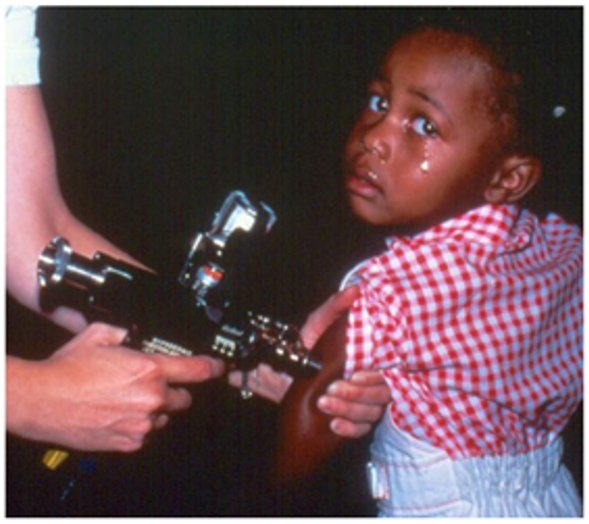
\includegraphics[width=0.35\textwidth]{chap2/images/original_injector.png}
                \label{fig:chapter/background/explain needle free/original injector}
            }
            \qquad
            \subfloat[Needle injection versus Needle-free injection\,\cite{injex2012}]{
                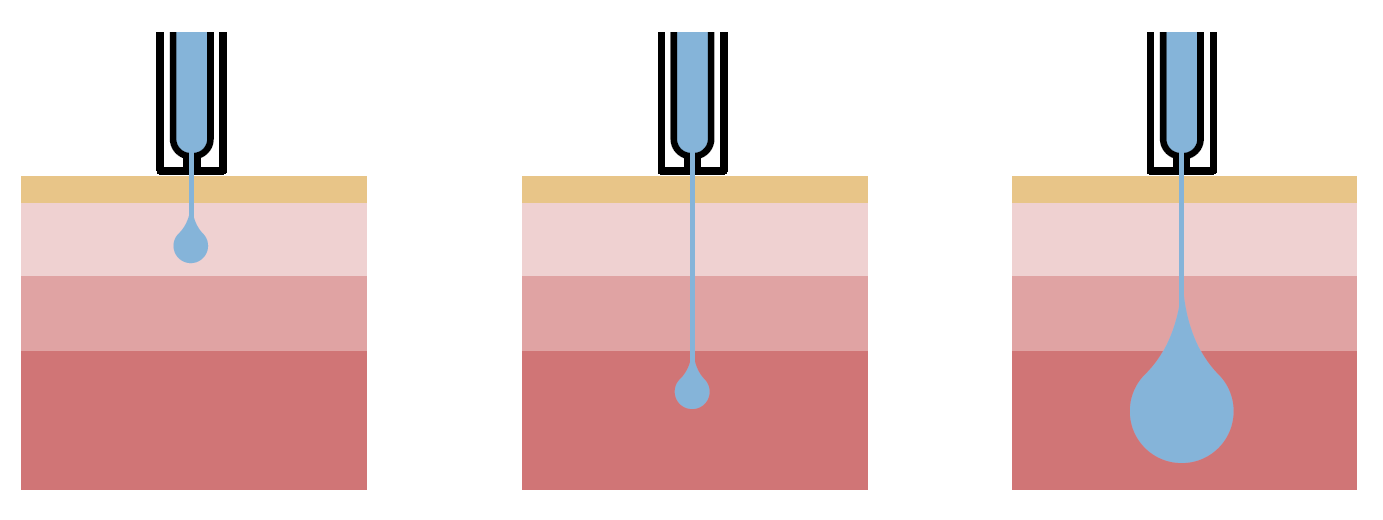
\includegraphics[width=0.5\textwidth]{chap2/images/needle_vs_needle_free.png}
                \label{fig:chapter/background/explain needle free/needle vs no needle}
            }
            \caption{
                Needle-free jet injection's history and concept explained.
            }   \label{fig:chapter/background/explain needle free}
        \end{figure*}
        
        A subcutaneous or intramuscular jet injection could be realized by forcing a fluid jet of $\mathrm{76-360\,\mu m}$  diameter to penetrate the human skin at a speed faster than $\mathrm{100 \,m/s}$\,\cite{mitragotri2006,Hogan2006}. Figure\,\ref{fig:chapter/background/explain needle free/needle vs no needle} shows that an ideal jet injection would deliver the drug in a similar manner to a hypodermic needle injection\,\cite{InsuJet2013}.
        
        % Even though this method adopts the use of needle-free apparatus, biological material can still be unwillingly transferred if there are no appropriate decontamination schemes. Concerns have been raised in the literature about potential transmission of blood-borne infections by multiple-use \acs{NFJI} since the early 1970s\,\cite{kremer1970, weintraub1988}. Figure\,\ref{fig:chapter/background/injection mechanism} illustrates three possible mechanisms of how blood contamination can take place\,\cite{hoffman2001}. 
        
        % \begin{figure*}[!ht]
    
        %     \centering
        %     \subfloat[]{
        %         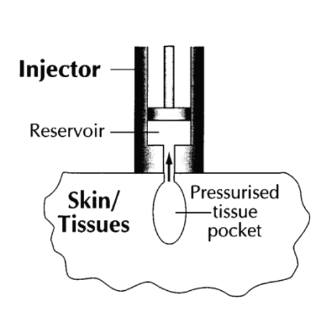
\includegraphics[width=0.29\textwidth]{chap2/images/jet_injection_mechanism_1.png}
        %         \label{fig:chapter/background/injection mechanism/1}
        %     }
        %     \subfloat[]{
        %         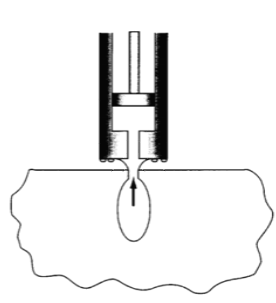
\includegraphics[width=0.25\textwidth]{chap2/images/jet_injection_mechanism_2.png}
        %         \label{fig:chapter/background/injection mechanism/2}
        %     }
        %     \subfloat[]{
        %         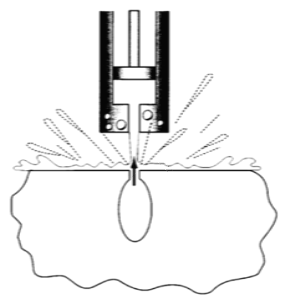
\includegraphics[width=0.27\textwidth]{chap2/images/jet_injection_mechanism_3.png}
        %         \label{fig:chapter/background/injection mechanism/3}
        %     }
        %     \caption{
        %         3 possible mechanisms of blood contamination in ‘mass campaign jet injectors’. 
        %     }   \label{fig:chapter/background/injection mechanism}
        % \end{figure*}    
        
        % Scenario in Figure\,\ref{fig:chapter/background/injection mechanism/1} shows that tissues return fluid into the reservoir as injection pressure diminishes. Liquid flows out to the tip of the injector as the injector’s tip is removed from the applied area as illustrated in Figure\,\ref{fig:chapter/background/injection mechanism/2}. Scenario in Figure\,\ref{fig:chapter/background/injection mechanism/3} displays a ‘splash back’ of jet stream during injection. Uninterrupted, continuous, reuse of \acs{NFJI} has historically caused instances of mass HBV spread\,\cite{canter1990}. For prevention of future mass infection, ‘mass campaign jet injectors’ were disapproved for human use by the World Health Organization\,\cite{who2005}. Nowadays, reusable \acsp{NFJI} for human use must accommodate replaceable syringes. 
    
    
    % -----------------------------------------------------------------------------------
    % --- NEW SUB SECTION --- NEW SUB SECTION --- NEW SUB SECTION --- NEW SUB SECTION --- 
    % -----------------------------------------------------------------------------------
    \subsection{Underlying mechanics}               \label{Chapter:background/needle-free jet injection/underlying mechanics}
    
        \begin{figure*}[!ht]
            \centering
            \subfloat[The general shape of jet penetration into polyacrylamide gel.]{
                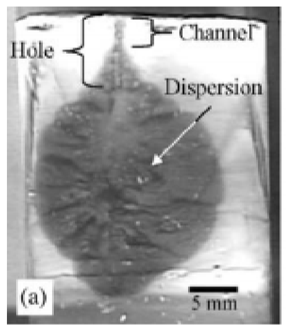
\includegraphics[width=0.28\textwidth]{chap2/images/jet_injection_mechanics_1.png}
                \label{fig:chapter/background/underlying mechanics/1}
            }
            \quad
            \subfloat[Side view of the same gel sample.]{
                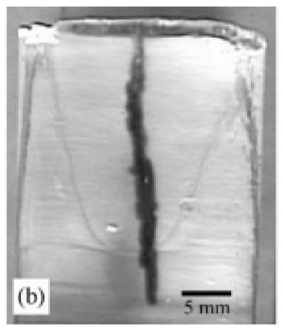
\includegraphics[width=0.28\textwidth]{chap2/images/jet_injection_mechanics_2.png}
                \label{fig:chapter/background/underlying mechanics/2}
            }
            \quad
            \subfloat[The transverse slice of the gel shows the presence of the cylindrical channel.]{
                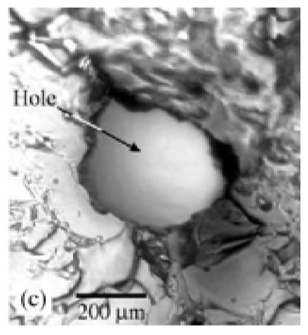
\includegraphics[width=0.3\textwidth]{chap2/images/jet_injection_mechanics_3.png}
                \label{fig:chapter/background/underlying mechanics/3}
            }
            \caption[Needle-free injection into a polyacrylamide gel containing $20\%$ acrylamide]{
                Needle-free injection into a polyacrylamide gel containing $20\%$ acrylamide\,\cite{schramm2004}.
            }   \label{fig:chapter/background/underlying mechanics}
        \end{figure*}
    
        To explore the mechanics of NFJI into the skin, an experiment was conducted where a high-speed camera monitored a spring-driven jet injection into polyacrylamide gel as a test bed\,\cite{Schramm-Baxter2004b} as shown in Figure\,\ref{fig:chapter/background/underlying mechanics}. Motion analysis demonstrated the presence of three distinct jet injection phases: erosion, stagnation, and dispersion. The erosion phase is the period when the jet penetrates in the form of a cylindrical channel. The brief reduction of upfront kinetic energy causes the fluid to start building up at a certain depth, described as the stagnation phase. The dispersion phase is where a drug volume infiltrates the cracks propagated within the gel by fluid pressure during previous phases. The maximum depth was controlled by altering the jet velocity at erosion, and likewise, the amount of drug delivered is determined by the jet speed at the dispersion phase\,\cite{Stachowiak2009}.
        
        
        \begin{figure*}[!ht]
            \centering
            \subfloat[]{
                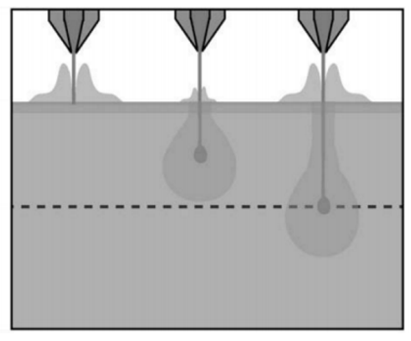
\includegraphics[width=0.515\textwidth]{chap2/images/1_speed_injection.png}
                \label{fig:chapter/background/2 speeds mechanics/just 1 speed}
            }
            \qquad
            \subfloat[]{
                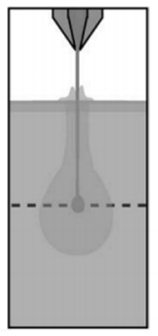
\includegraphics[width=0.20\textwidth]{chap2/images/2_sppeds_injection.png}
                \label{fig:chapter/background/2 speeds mechanics/2 speeds}
            }
            \caption[Need for temporal control of jet velocity in needle-free transdermal drug delivery: (a) constant low-velocity delivery (left), medium-velocity delivery (centre), and high-velocity delivery (right); (b)Desired drug delivery showing sufficient penetration depth and minimal pooling. Dotted line represents the desired depth of injection.]{
                Need for temporal control of jet velocity in needle-free transdermal drug delivery\,\cite{Mitragotri2005}: (a) constant low-velocity delivery (left), medium-velocity delivery (centre), and high-velocity delivery (right); (b)Desired drug delivery showing sufficient penetration depth and minimal pooling. Dotted line represents the desired depth of injection.
            }   \label{fig:chapter/background/2 speeds mechanics}
        \end{figure*}
        
        
        Difficulty in controlling depth injection and ‘splash back’ were the result of using a single jet velocity\,\cite{schramm2002}. Figure\,\ref{fig:chapter/background/2 speeds mechanics/just 1 speed} explains the need for temporal control of the jet velocity in needle-free transdermal drug delivery\,\cite{Mitragotri2005}. At constant low pressure, the jet may not penetrate into the skin (left), while constant, medium-pressure jet velocity may breach the skin with minimal ‘splash back’ yet reach an insufficient depth (middle). A high-pressure stream may reach the desired depth, but fluid pooling cannot be avoided (right). With the use of an initial high jet pressure followed by a lower holding pressure, it was predicted that ’splash back’ would be reduced while the jet disperses at the correct depth\,\cite{wendell2006}. This concept is portrayed in Figure\,\ref{fig:chapter/background/2 speeds mechanics/2 speeds} and \ref{fig:chapter/background/2 speeds ideas}. Taberner et al.\,\cite{taberner2012} demonstrated that the use of a high degree of fluid stream velocity control can deploy this strategy reliably.
        
        
        \begin{figure}[h]
            \centering
            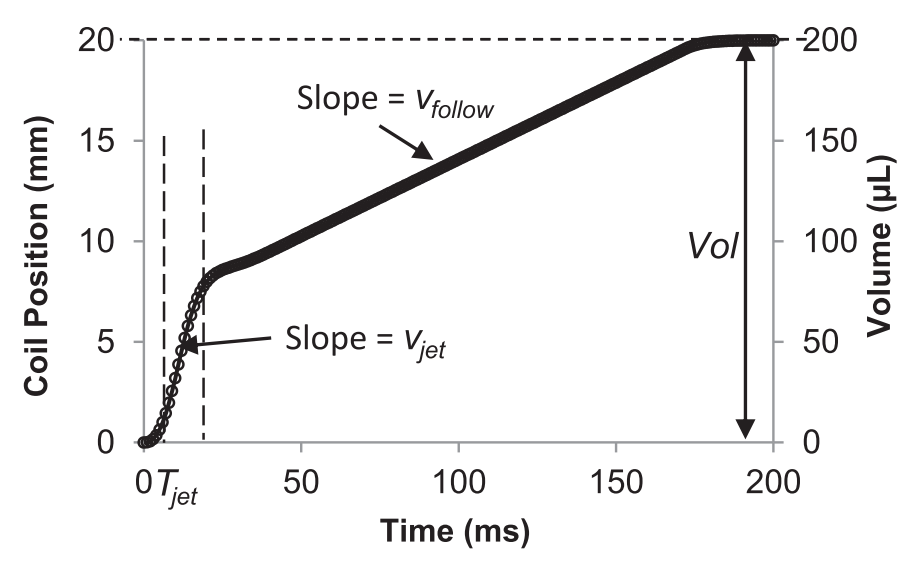
\includegraphics[width=0.75\textwidth]{chap2/images/2_jet_speeds_idea.png}
            \caption[A typical 2 speeds jet injection trajectory; $v_{jet}=200\,\mathrm{m/s}$ to reach the desired injection depth and $v_{follow}=20\,\mathrm{m/s}$ to reduce ‘splash back’]{A typical 2 speeds jet injection trajectory; $v_{jet}=200\,\mathrm{m/s}$ to reach the desired injection depth and $v_{follow}=20\,\mathrm{m/s}$ to reduce ‘splash back’ \,\cite{taberner2012}}
          \label{fig:chapter/background/2 speeds ideas}
        \end{figure}
    
    
    % -----------------------------------------------------------------------------------
    % --- NEW SUB SECTION --- NEW SUB SECTION --- NEW SUB SECTION --- NEW SUB SECTION --- 
    % -----------------------------------------------------------------------------------
    \subsection{Commercially available options}     \label{Chapter:background/needle-free jet injection/commercially available options}
        
        Commercially available \acsp{NFJI} including BIOJECT Zeajet\footnote{http://www.bioject.com/products/zetajet-info} , INJEX 30\footnote{https://www.injex.com.au/injex/injex} , PHARMAJET Stratis\footnote{http://pharmajet.com/fda-approved-needleless-flu-shot} , COMFORT-IN\footnote{http://www.comfort-in.com/diabetes.html}  are spring-powered, small, portable, handheld devices. They are capable of delivering either vaccination or insulin in a small dose, with volume limited to $\mathrm{300\,\mu L}$. Figure\,\ref{fig:chapter/background/pharma jet stratis} illustrates the appearance, construction, and mechanism of the spring-loaded PHARMAJET Stratis NFJI as an example. These devices come in various shapes, sizes, injection volumes, and target skin layers. Their primary structure consists of three main components:
        \begin{itemize}
            \item Energy storage - compressed gas, spring coil or explosives\,\cite{taberner2012}, which are often accompanied by a recharging device,
            \item Piston - actuator with various size and triggering method to accomplish desired pressure profile as well as injection volume specification,
            \item Replaceable syringe - single use container with orifice hole diameter of under $\mathrm{1\,mm}$.
        \end{itemize}
        
        \begin{figure*}[!ht]
            \centering
            \subfloat[\acs{NFJI} device and replaceable syringe]{
                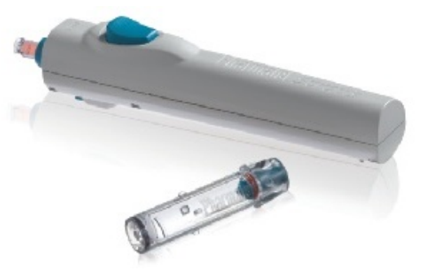
\includegraphics[width=0.40\textwidth]{chap2/images/pharma_jet_stratis.png}
                \label{fig:chapter/background/pharma jet stratis/full view}
            }
            \qquad
            \subfloat[Spring loaded mechanism of the device]{
                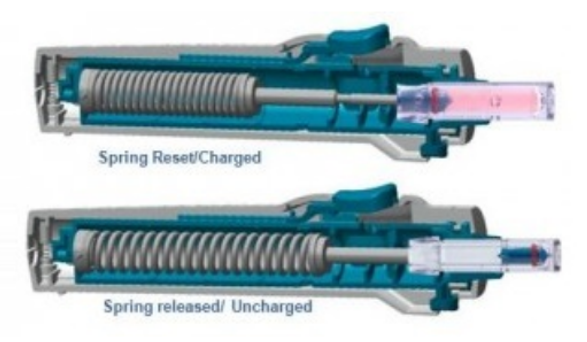
\includegraphics[width=0.45\textwidth]{chap2/images/pharma_jet_stratis_cut_view.png}
                \label{fig:chapter/background/pharma jet stratis/cut view}
            }
            \caption[SUNFJI Pharma Jet Stratis™ from PharmaJet™]{
                SUNFJI Pharma Jet Stratis™ from PharmaJet™\,\cite{PharmaJet2011}
            }   \label{fig:chapter/background/pharma jet stratis}
        \end{figure*}
        
        Once triggered, stored energy produces varying pressure on the injection cylinder until the piston reaches the end of its track. Different devices utilize different recoil or trigger mechanisms, but no system is capable of monitoring and measuring injection performance. Instead of concentrated fluid delivery in a narrow stream down the tissue, these devices tend to spread the drug content in a cone shape\,\cite{baxtex2005}. Figure\,\ref{fig:chapter/background/jet injection effectiveness/mechanical devices pressure curve} shows the sharp peak and oscillating nature of the pressure produced by the injection stream of a BIOJECT Vitajet 3™ spring powered \acs{NFJI}\,\cite{schramm2002}. Schneider et al.\,\cite{schneider1994} reported that without stroke velocity and position control, the sharp fluid pressure profile peak could cause pain, bruises, bleeding, and blisters. Their studies also showed evidence that the same spring powered NFJI device exhibits inconsistent performance across different skin types and conditions. 
        
        Despite being a safer alternative, mechanically powered \acsp{NFJI} require manual recharging. Thus, the average cycle time was recorded to be no faster than that of a conventional hypodermic needle injection\,\cite{PharmaJet2011}. More advanced \acsp{NFJI} like LECTRAJET  have shown the capability of automatic spring recoil to reduce reload time. Lack of pressure control, low injection volume (typically $0.05$ to $0.3\,\mathrm{mL}$), long cycle time, poor repeatability and reproducibility are drawbacks of commercially available mechanically powered \acsp{NFJI}.
        
        \begin{figure*}[!ht]
            \centering
            \subfloat[Typical pressure curve for a $152\,\mathrm{\mu m}$ diameter nozzle from injector Vitajet\,3™]{
                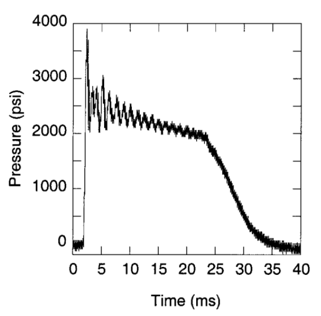
\includegraphics[width=0.43\textwidth]{chap2/images/jet_injection_pressure_curve.png}
                \label{fig:chapter/background/jet injection effectiveness/mechanical devices pressure curve}
            }
            \qquad
            \subfloat[Delivery of mannitol by jet injection into human (A), porcine abdominal (B), and porcine dorsal skin (C) using the same device at $177\,\mathrm{m/s}$. There is a significant difference between each type of skin tested ($p=0.001$)]{
                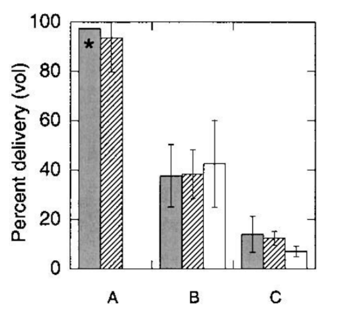
\includegraphics[width=0.45\textwidth]{chap2/images/jet_injection_delivery_study.png}
                \label{fig:chapter/background/jet injection effectiveness/delivery statistic}
            }
            \caption[Results of different jet injection study on mechanically powered \acs{NFJI} devices demonstrating rough pressure profile and poor adaptability.]{
                Results of different jet injection study on mechanically powered \acs{NFJI} devices demonstrating rough pressure profile and poor adaptability\,\cite{schramm2002}.
            }   \label{fig:chapter/background/jet injection effectiveness}
        \end{figure*}


    % -----------------------------------------------------------------------------------
    % --- NEW SUB SECTION --- NEW SUB SECTION --- NEW SUB SECTION --- NEW SUB SECTION --- 
    % -----------------------------------------------------------------------------------
    \subsection{Controllable \acs{NFJI} devices}    \label{Chapter:background/needle-free jet injection/Controllable NFJI}
    
        Recent achievements in high power density actuators have enabled successful prototypes of electronically controlled \acsp{NFJI} which were capable of real-time jet velocity control. A previous study suggests four advantages of electronic control over traditional needle injection and mechanically powered jet injection\,\cite{henmond2013}:
        
        \begin{itemize}
            \item Controllable - capable of maintaining high pressure without the need of trading-off for injection volume,
            \item Reliable - capable of producing consistent jet pressure on a broad range of skin properties and different injection types,
            \item Versatile - automatic reload under closed loop control or injection volume control,
            \item Measurable - convenient in monitoring progress to evaluate the performance of injection.
        \end{itemize}
        
        This class of device performs injections by utilizing different electrically powered actuators: dynamically controlled piezo-electric actuators\,\cite{Stachowiak2009}, laser pulsed microjets\,\cite{tawaga2013, park2012} and Lorentz force voice coil motors\,\cite{taberner2006,hemond2006}. Piezo-electric and laser pulse methods are limited to sub $\mathrm{\mu L}$ injections. Scaling of Piezo-electric technology to hundreds of $\mathrm{mL}$ range in injection volume simply appears ambitious. Cumbersome ‘off-the-shelf’ voice coil actuators which will be explored in \ref{Chapter:background/voice coil motors for NFJI} are not yet suitable to become handheld. Recently, Zhang et al. has shown a \acs{NFJI} device powered by commercial rotary motor and specialized differential screw structure, capable of delivering $10\,\mathrm{\mu L}$ with the input power of $450\,\mathrm{W}$\,\cite{Zhang2017Needle-freeActuator}. Although the concept of utilizing synchronous rotary motor for \acs{NFJI} was proven, the volume delivered that a similar system could achieve will be unlikely to reach $1\,\mathrm{mL}$.

% ===================================================================================================
% === NEW SECTION === NEW SECTION === NEW SECTION === NEW SECTION === NEW SECTION === NEW SECTION ===
% ===================================================================================================
\section{Voice coil motors for \acs{NFJI}}          \label{Chapter:background/voice coil motors for NFJI}
    
    
    % -----------------------------------------------------------------------------------
    % --- NEW SUB SECTION --- NEW SUB SECTION --- NEW SUB SECTION --- NEW SUB SECTION --- 
    % -----------------------------------------------------------------------------------
    \subsection{Principle of operation}             \label{Chapter:background/voice coil motors for NFJI/principle}


    The \ac{VCM} is a type of Lorentz-force actuator. \acsp{VCM} can either have the magnet or the coil as a moving part. Figure\,\ref{fig:chapter/background/vcm cut view} presents the construction of a moving coil configuration\,\cite{taberner2006}. Here, a Nd-Fe-B magnet is used to generate the magnetic field. The magnet is placed between a steel top plate and the steel casing to direct the flow of magnetic flux in a contained loop. In between the top plate and steel case is a region of air gap that allows the copper winding to slide up or down. A directional force $F$ is proportional to the strength of the magnetic field $B$ through the wire, and the electric current per unit area $J$ passing through the coil:
    
    
    \begin{equation}
        \overrightarrow{F}=\overrightarrow{J}\times \overrightarrow{B}
        \label{eq:force produce via field and current}
    \end{equation}

    The polarity of the current also dictates which direction the coil will move. It is clear that more force can be generated by either strengthening the magnetic field or increasing the current through the coil. Adjusting other parameters such as coil geometry, coil thickness, magnet materials, and aspect ratio can alter the motor force constant and stroke length.
    
    
    \begin{figure}[!ht]
      \centering
      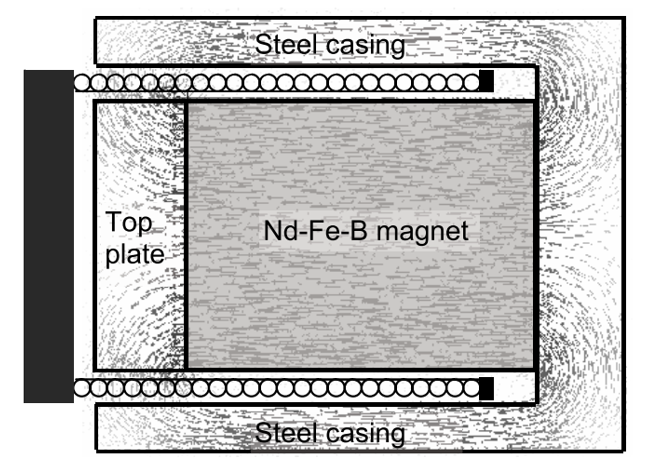
\includegraphics[width=0.5\textwidth]{chap2/images/vcm_cut_view.png}
      \caption[Construction of a voice coil motor with moving coil]{Construction of a voice coil motor with moving coil\,\cite{taberner2006}.}
      \label{fig:chapter/background/vcm cut view}
    \end{figure}
    
    
    % -----------------------------------------------------------------------------------
    % --- NEW SUB SECTION --- NEW SUB SECTION --- NEW SUB SECTION --- NEW SUB SECTION --- 
    % -----------------------------------------------------------------------------------
    \subsection{Application to \acs{NFJI}}          \label{Chapter:background/voice coil motors for NFJI/application}
    
    
    Recently, collaboration between the \ac{MIT} and \ac{ABI} Bioinstrumentation Labs has created two prototype jet injectors actuated by a customized Lorentz-force \ac{VCM}\,\cite{taberner2006,ruddy2014} shown in Figure\,\ref{fig:chapter/background/vcm injectors}. With the use of real-time feedback control, these systems have demonstrated highly controllable and repeatable injections against a broad range of different test tissues, depths, and dosage volumes\,\cite{taberner2012}. With the successful prototypes, the vision was to advance the prototypes into portable and high volume injector devices.


    \begin{figure*}[!ht]
        \centering
        \subfloat[]{
            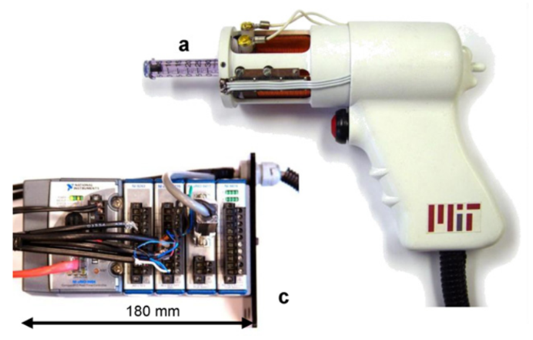
\includegraphics[width=0.5\textwidth]{chap2/images/vcm_taberner2006.png}
            \label{fig:chapter/background/vcm injectors/taberner2006}
        }
        \qquad
        \subfloat[]{
            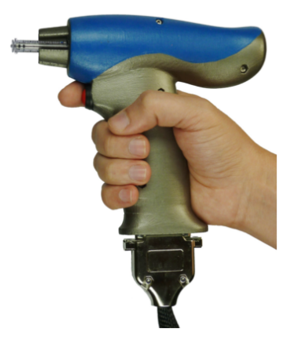
\includegraphics[width=0.28\textwidth]{chap2/images/vcm_ruddy2014.png}
            \label{fig:chapter/background/vcm injectors/ruddy2014}
        }
        \caption[Lorentz-force VCM actuated NFJI: Handheld injector and cRIO controller system (a); Hand-held injector and charged capacitor amplifier/controller system (b).]{
            Lorentz-force VCM actuated NFJI: Handheld injector and cRIO controller system (a)\,\cite{taberner2006}; Hand-held injector and charged capacitor amplifier/controller system (b)\,\cite{ruddy2014}.
        }   \label{fig:chapter/background/vcm injectors}
    \end{figure*}
    
    
    \begin{figure}[!ht]
      \centering
      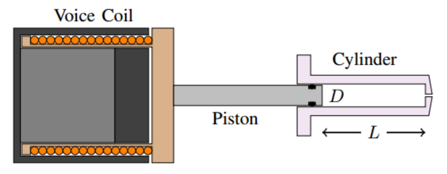
\includegraphics[width=0.5\textwidth]{chap2/images/vcm_for_nfji.png}
      \caption[A basic schematic of a voice coil actuated NFJI. $L$ and $D$ are the cylinder’s working length (stroke length) and diameter, respectively.]{A basic schematic of a voice coil actuated \acs{NFJI}. $L$ and $D$ are the cylinder’s working length (stroke length) and diameter, respectively\,\cite{ruddy2014}.}
      \label{fig:chapter/background/vcm for nfji}
    \end{figure}
    
    
    Figure\,\ref{fig:chapter/background/vcm for nfji} shows a basic schematic of a voice coil actuated \acs{NFJI}. $L$ and $D$ are the cylinder’s working length (stroke length) and diameter, respectively\,\cite{ruddy2014}. In this device, injection volume can be enlarged by either up-scaling the ampoule diameter $D$, or the working stroke length $L$, or both. A jet injector with an ampoule diameter $D$ requires an actuation force $F$ to be provided by the motor. For constant peak jet velocity $v_{jet}$ and fluid density $\rho$:
    
    
    \begin{equation}
        F=\frac{\pi}{8}\rho {v_{jet}}^2 D^2
        \label{eq:force produce relationship in motor powered NFJI}
    \end{equation}
    
    
    If syringe’s diameter\,$D$ is chosen to scale with injection volume, electric power\,$P$ needs to scale with the square of $D$’s scaling ratio due to the relationship:
    
    
    \begin{equation}
        P=F v_{piston}
        \label{eq:power required for F and v_piston}
    \end{equation}
    
    
    where $v_{piston}$ is the speed of the moving piston. If the syringe’s diameter  is chosen to scale with the injection volume, the electric power\,$P$ needs to scale with the square of $D$’s scaling ratio. Given that the jet velocity follows the varying velocity strategy explained in Section\,\ref{Chapter:background/needle-free jet injection/underlying mechanics}, the motor needs to achieve the peak jet velocity required for the brief erosion phase, then the lower jet velocity speed for the dispersion phase. For only for a very short period, the device is required to produce much more power than its average power drawn. It is not common to find energy storage and powering devices at power magnitude of many kilowatts, provided in a portable fashion.
    
    
    % -----------------------------------------------------------------------------------
    % --- NEW SUB SECTION --- NEW SUB SECTION --- NEW SUB SECTION --- NEW SUB SECTION --- 
    % -----------------------------------------------------------------------------------
    \subsection{Scaling properties and limitations} \label{Chapter:background/voice coil motors for NFJI/scaling and limitation}
    
    
    The following key relationship relates the power dissipation on the motor winding $P$, density of fluid to be delivered $\rho$, ampoule volume $V$, jet velocity $v_{jet}$, motor constant $K_m$, and distance travelled by the piston stroke $L$ \cite{Williams2012}:
    
    
    \begin{equation}
        P=\frac{\rho^2 V^2 {v_{jet}}^4}{4 {K_m}^2 L^2}
        \label{eq:power required for F,V,v_jet,K_m, and L}
    \end{equation}
    
    
    To compare the force exerted over the power consumed in different motors, the motor constant $K_m$ measured in $\mathrm{N/\sqrt{W}}$  is typically used. Note that this relationship is true of all direct drive linear motors, which apply force directly to a single injection ampoule without any mechanical coupling transmission.
    
    
    Utilizing a general scaling magnetic and thermal model made for steady-state force production of \ac{PMLSM}\,\cite{Ruddy2011}, an optimal \acs{VCM} hand-piece was built to deliver $\mathrm{300\,\mu L}$ of the drug over a $\mathrm{50\,ms}$ period\,\cite{taberner2006}. The peak power required for this procedure was as high as 10 kW to produce a peak force of $\mathrm{300\,N}$ of over the stroke length of $\mathrm{35\,mm}$. Due to the extremely short duration of the force profile, the heat generated is far from enough to cause permanent demagnetization in the permanent magnet array; thus, the motor design neglects heat transfer. In the same body of work, the authors pointed out that scaling laws of the voice coil actuator fit for needle free injection means that the power $P$ required and motor mass $M$ both grow faster than the injection volume $V$:
    
    
    \begin{equation}
        M \propto V^{6/5}
        \label{eq:scaling property of VCM}
    \end{equation}


    While the potential of using \acsp{VCM} in portable \acs{NFJI} devices has been proven, this type of motor is power inefficient. Without breakthrough improvements, \acsp{VCM} pose a considerable restriction on the portability of the electronic control system, as well as the size of the injector handpiece motor. Based on the model presented in that work, a \acs{VCM} with mass of over $\mathrm{1\,kg}$ is required to deliver $\mathrm{1\,mL}$. Thus, it was impractical to use a direct-drive linear \acs{VCM} to deliver regular livestock injections, where the volume can be as high to $\mathrm{10\,mL}$. 

% ===================================================================================================
% === NEW SECTION === NEW SECTION === NEW SECTION === NEW SECTION === NEW SECTION === NEW SECTION ===
% ===================================================================================================
\section{Linear synchronous motors for NFJI}        \label{Chapter:background/linear synchronous motors for NFJI}

    
    \acp{LSDDM} are actuators that can drive a motion load without an intermediate mechanism such as gears, screws or crank shafts\,\cite{JacekF.GierasZbigniewJ.Piech2017}. The absence of auxiliary mechanical adaptation increases their reliability. In high speed applications, linear direct-drive synchronous motors can have higher efficiency and a higher dynamic performance compared to their rotary counter parts. ‘Synchronous’ in the context of electric machines means that the speed of motion is the same as the speed of the travelling magnetic field. The thrust is generated by either the interaction between the traveling magnetic field produced by the poly-phase winding or switched DC windings in an array of magnetic excitation components. 
    
    \acsp{LSDDM} are being used increasingly in applications as varied as automated manufacturing\,\cite{Meessen2010}, transportation\,\cite{Gysen2011,Cao2012,WenxiangZhao2012}, and power generation\,\cite{Li2011,Baker2019}. Although \acsp{LSDDM} have existed for a long time\,\cite{Boldea1997}, to the best of the author’s knowledge, no report has demonstrated that this class of motor can achieve \acs{NFJI} tasks, where a high pulse of force is required from a near stall condition. Technically speaking, a \acs{VCM} is a type of \acs{LSDDM} where there is a single-phase winding driven by a direct current and an array of magnetic excitation with length equal one pole period. True linear synchronous motors, powered by alternating current, provide efficient energy to motion conversion, high force density and excellent capability for precise motion control\,\cite{Trumper1994,Levi1973,Budig2000}.
    
    
    % -----------------------------------------------------------------------------------
    % --- NEW SUB SECTION --- NEW SUB SECTION --- NEW SUB SECTION --- NEW SUB SECTION --- 
    % -----------------------------------------------------------------------------------
    \subsection{Classification}                     \label{Chapter:background/linear synchronous motors for NFJI/classification}
    
        
        The most basic motor consists of two principal components\,\cite{JacekF.GierasZbigniewJ.Piech2017}: the part that produces the travelling magnetic field via a poly-phased copper winding is the armature, and the part that produces magnetic flux or variable reluctance is known as the field excitation system (e.g., a permanent magnet or magnetic field created by induction). \acsp{LSDDM} can come in many different topologies\,\cite{Laithwaite1970}:
        
        
        \begin{itemize}
            \item Moving or fixed armature
            \item Flat (planar) or tubular (cylindrical)
            \item Ferromagnetic core or air core
            \item Slotted or slot-less core (if using back iron core)
            \item Permanent magnet excitation or electromagnetic excitation
            \item Longitudinal flux or transversal/transverse flux
            \item Singly salient or doubly salient
        \end{itemize}
        
        
        Moving or fixed armature simply refers to which part of the motor moves, be it the part containing the armature or part that contain the field excitation system. A moving armature system requires more materials for the fixed field excitation system, which often increases the demand for costly rare-earth permanent magnets. In contrast, the a moving field excitation system often leads to more demanding electronics to control more armature phases. The moving armature configuration is more commonly seen in linear direct drive motors. 
        
        
        The tubular motor concept can be realized by rolling a flat linear machine about its longitudinal axis. Tubular permanent-magnet machines offer the highest efficiency and power over force density and have excellent servo characteristics\,\cite{Eastham1990}. The advantages that the tubular structure can offer over the flat structure includes introducing even magnetic field distribution, reducing wasted winding, and easing the modelling step. Despite superior performance, tubular machines are only more popular than flat machines in research because they are more difficult to manufacture at scale.
        
        
        The ferromagnetic core, whether it is a magnet core or an iron core, exists to provide a low magnetic resistance path between the excitation source and the armature. The subset of \ac{PM} synchronous motors with the use of an iron core has to deal with cogging force. This force stands for the mutual attraction between the PM and iron in the armature. Cogging force is undesirable because it can contribute to a reduction in axial force, vibration and deteriorating control characteristics at low speed\,\cite{Jung1999}. The slotted iron core causes the cogging ripples while the limited iron length causes end effect cogging\,\cite{Lim2002}. Cogging force can be reduced by PM width adjustment\,\cite{Bianchi2002}, asymmetric PM arrangement\,\cite{Chung2016,Bianchi2003a,Cai2012}, a semi-closed slot for the iron core\,\cite{Zhu1997,Bai2015,Zhu2008}, and optimizing iron core geometry\,\cite{Inoue2000,Zhu1997,Wu2008,Zhu2009conf,Zhang2013,Kim2016,Lee2014}. It is better to improve the cogging force profile using mechanical design than to rely on complex control mechanism\,\cite{Jahn1996}. 
        
        
        Recently, the number of research on actuators using permanent magnets has increased significantly. This is due to the availability of high energy rare earth permanent magnet materials from which compact actuators with a high efficiency can be realized. As the size approaches the form factor required for power application such as electric vehicle or energy generation, the difference in performance of induction and permanent magnet machines is small\,\cite{WoosukSung2012Energy-EfficientVehicles,2014Almeida,Chau2008OverviewVehicles,deSantiago2012ElectricalReview}. However, in small form factor use-cases, permanent magnet machines have been reported to outperform induction machines\,\cite{Zhu2007ElectricalVehicles,Yang2015ComparativeApplications}. 
        
        
        The most important distinction for motors perhaps lies in the arrangement of the flux path. Longitudinal flux means that the magnetic field lines are parallel to the direction of motion. Transverse flux, on the other hand, means that the magnetic field lines are perpendicular to the direction of the motion\,\cite{Laithwaite1975}. Further definition of \acfp{LTFM} includes having three-dimensional magnetic flux flow, and there is no coupling between the individual armature and secondary phases. \acsp{LTFM} are especially suitable for low speed and high thrust applications\,\cite{Zhao2015,Shin2015}. This topology allows for containing a large number of poles without compromising the space available for the windings\,\cite{Laithwaite1971}. The structure of this type of motor results in a complex, coupled magnetic and electric circuit. An increase in the number of poles is roughly proportional to the increase in force density. A transversal flux motor, in both rotary and linear forms, can achieve very high work output\,\cite{Ueda2014,Hsu2011,Wang2016,Arshad2001,Siatkowski2008}. Longitudinal flux machines may have discrete structural poles, but for transversal flux machines, discretization of the poles is compulsory\,\cite{Baoming2009}. This structure offers easier and cheaper design, manufacturing and maintenance. However, the segmented core construction and widely open conductor loop lead to high leakage flux, high winding inductance, and low power factor\,\cite{Harris1997,Lu2003}. The iron core takes significantly more volume and weight in transversal flux motors, thus, eddy losses and nonlinear permeability effects must be included to model this type of motor accurately.
        
        
        Both transverse flux motors, or longitudinal flux when called alone, refers to motors that have the flux source (\acs{PM} for instance) separated from the current source, and both sources will not move at the same time as the motor operates. Since the flux source interacts with the current source through an air gap without hard mechanical coupling, we refer to those motors as singly salient motors. On the other hand, doubly-salient motors have "teeth" on both the primary and secondary, resulting in both sides contributing to variation in flux linkage/inductance with position. Belonging  to  the  the  family of doubly-salient permanent magnet motors \,\cite{Cheng2011}, \acp{LFSM} have high  thrust  density, high  tolerance  to  current  overload, lower use  of  permanent  magnet  material,  and  a generally robust construction. They use a passive secondary that can be made out of steel laminations or \ac{SMC} material to reduce eddy current loss to a minimum. Being  able  to ignore eddy currents will play an important role in improving the efficiency of design simulation. The amount of \acs{PM} in a \acs{LFSM} in long stroke applications can be significantly less than that used by a \acs{PMLSM}\,\cite{Aleksandrov2018}. All these advantages are important in bringing a  prototype into manufacturing at scale to reach high reliability. In hindsight, air is a very poor magnetic conductor, thus machines like \acsp{LFSM} with very small flux path resistance should vastly improve motors output. However, since the \acs{LFSM} is still a relatively unexplored topology, the literature has opposing opinions about whether \acsp{LFSM} outperform \acsp{PMLSM}\,\cite{Aleksandrov2018,Wang2008}.
        
        
        One of the disadvantages of synchronous motors is that once the motion and rotating magnetic fields were out synchronism, the motors would not move. A way to work around this problem is to incorporate absolute position sensors or Hall sensors into the control algorithm of the motor. In some cases where the armature requires a large starting torque, the motor is inherently unable to start itself. Even with the help of methods to speed up to synchronism, the armature can always lag if the power supplied is insufficient to cope with the load.
        
        
        Compared to \acsp{VCM}, \acsp{PMLSM} and \acsp{LFSM} in general require far less power to operate. Thus, the same portable power supply built for powering \acsp{VCM} is also capable of driving the other \acsp{PMLSM} and \acsp{LFSM}, provided the technology used has room to expand for multiphase control.
        
        
    % -----------------------------------------------------------------------------------
    % --- NEW SUB SECTION --- NEW SUB SECTION --- NEW SUB SECTION --- NEW SUB SECTION --- 
    % -----------------------------------------------------------------------------------
    \subsection{Summary}                         \label{Chapter:background/linear synchronous motors for NFJI/summary}
        
        
        Previous work at the ABI also conceived a design of a \ac{PMLSM} optimized for \acs{NFJI} application\,\cite{Ruddy2015}. The motor described in that work is a moving armature, tubular, single-sided, back iron cored, slot-less, \acs{PM}, and longitudinal flux linear synchronous motor. The optimized tubular \acs{PMLSM} with a stroke length of $\mathrm{200\,mm}$ and an injection volume of $\mathrm{1\,mL}$ promised a drastic reduction in power requirement compared to \acsp{VCM}. The next step from there is to construct a prototype motor and power amplifier and incorporate them into a complete \acs{NFJI} system. Such motor design will need to incorporate a creative packaging strategy to maintain the hand-held nature of the \acs{NFJI} device. The challenges of constructing \acs{PMLSM} motors with use of PM also include assembly of a large number of small and mutually attracted parts\,\cite{Hwang2012,Shin2012}.
        
        
        While the scaling law of longitudinal flux \acs{PMLSM} requires the stroke length to be long to make a drastic improvement in power efficiency\,\cite{Laithwaite1970}, that is not the case in transversal flux motors. The implication is that the uses of long \acs{NFJI} ampoule strokes and cumbersome packaging mechanism can be avoided altogether if we decided to adopt linear transversal flux motors. The use of newer types of motor such as \acsp{LFSM} should also be explored because it is possible to save a significant amount of rare-earth permanent magnet and have near equivalent performance to \acs{PMLSM}.


% ===================================================================================================
% === NEW SECTION === NEW SECTION === NEW SECTION === NEW SECTION === NEW SECTION === NEW SECTION ===
% ===================================================================================================
\section{Electromagnetic field theory}              \label{Chapter:background/electromagnetic field theory}


    The emergence of energy convergence of energy conversion applications and modern electronics have led to a large variety of magnetic materials supplied in all shapes and size. The phenomenon of a material forming a permanent magnet or temporary microscopic dipoles under the influence of a magnetic field is known as ferromagnetism. While all materials are magnetic to some extent, only ferromagnetic materials can form strong magnetic flux density $B$ under the influence of an external magnetizing field $H$. In this body of work, they are referred as ‘$B$-field’ and ‘$H$-field’. 
    

    % -----------------------------------------------------------------------------------
    % --- NEW SUB SECTION --- NEW SUB SECTION --- NEW SUB SECTION --- NEW SUB SECTION --- 
    % -----------------------------------------------------------------------------------
    \subsection{Quasi-static Maxwell's equations}     \label{Chapter:background/electromagnetic field theory/quasi-static maxwell equations}
    
    
        Maxwell's equations describe how electric and magnetic fields are generated by charges, current, and the changes in either magnetic or electric fields. As a set of \acp{PDE}, they provide a foundation for understanding classical electromagnetism, optics and even electrical circuits. In the case of motors, the electromagnetic fields travel drastically slower than the maximum speed possible for electromagnetic waves, known as the speed of light. The time rates of changes of relevant electromagnetic fields are sufficiently low that they can be simplified to the set of quasi-static Maxwell's equations\,\cite{Melcher1981}. The quasi-static Maxwell's equations in differential forms are defined as:
    
    
        \begin{equation}
            \nabla \times H = J_f
            \label{eq:ampere's circuit law}
        \end{equation}
        
        \begin{equation}
            \nabla \cdot B = 0
            \label{eq:gauss's magnetism law}
        \end{equation}
        
        \begin{equation}
            \nabla \times E = \frac{\partial B}{\partial t}
            \label{eq:maxwell-faraday's law}
        \end{equation}
    
        \begin{equation}
            \nabla \cdot D = \rho
            \label{eq:gauss's law}
        \end{equation}
    
    
        where $J_f$ is the free current density in the conductor, $E$ is the electric field, $D$ is the electric flux density and $\rho$ is the free electrical charge destiny. Bold symbols here represent vector quantities. Even existing in a simplified form, these equations are coupled \acsp{PDE}, which are often very difficult to solve analytically. Like any differential equation, boundary conditions and initial conditions are necessary for a unique solution. Numerical methods can be used to approximate the result, but an exact solution is not yet found.
        
        
        The Maxwell's equations can be rewritten to by introducing the magnetic vector potential $A$, free space permeability ${\mu}_0$, and the conductor relative permeability ${\mu}_r$, true for quasi-static conditions:
        
        
        \begin{equation}
            \nabla \times A = B
            \label{eq:curl of A is B}
        \end{equation}        
        
        \begin{equation}
            M = M_0 + M_f
            \label{eq:component of magnetization}
        \end{equation}     
        
        \begin{equation}
            {\nabla}^2 A = -{\mu}_0 ({\mu}_r J_f + \nabla \times M_0)
            \label{eq:relation of A to Magnetization and free current}
        \end{equation}        
        
        
        The magnetization $M$ of a ferromagnetic material has two components. The first magnetization component $M_0$ results from permanent magnetization in hard magnetic material like permanent magnets. The secondary magnetization $M_s$ is related to the magnetic field $H$, which can be temporary:
        
        
        \begin{equation}
            M_s = \chi_m H
            \label{eq:secondary magnetization}
        \end{equation}     
        
        
        where $\chi_m$ is the magnetic susceptibility that can be a function of $H$ in non-linear materials. In a special case where there is no free current density, the magnetic scalar potential $\varphi$ is defined as:
        
        
        \begin{equation}
            - \nabla \varphi = H
            \label{eq:magnetic scalar and vector potential}
        \end{equation}     
        
        \begin{equation}
            \nabla^2 \varphi = \frac{1}{\mu_r} \nabla \cdot M_0
            \label{eq:magnetic scalar magnetization}
        \end{equation}     
        
        
        Note that Equation \ref{eq:relation of A to Magnetization and free current} and Equation \ref{eq:magnetic scalar magnetization} takes the form of the Poisson equation. The advantage of scalar potential is the reduced complexity compared to vector potential, which requires solving three-dimensional vector equations.
        
        
    % -----------------------------------------------------------------------------------
    % --- NEW SUB SECTION --- NEW SUB SECTION --- NEW SUB SECTION --- NEW SUB SECTION --- 
    % -----------------------------------------------------------------------------------
    \subsection{Ferromagnetic materials}                \label{Chapter:background/electromagnetic field theory/ferromagnetic material theory}
    
    
        The microscopic local magnetic alignment via dipoles spinning in ferromagnetic materials leads to the formation of magnetic ‘domains’. These are ‘hard’ ferromagnetic materials, and it is rather difficult to magnetize or demagnetize them. The reason is that the intrinsic material properties strongly resist the movement of domain walls. On the other hand, ‘soft’ ferromagnetic materials are easy to magnetize or demagnetize because the domain wall movement does not require a strong external $H$-field. The most common example of ‘soft’ magnetic behaviour is when a piece iron is attracted to a permanent magnet, the iron piece itself becomes temporarily magnetized to the extent that it can attract other iron pieces. 
        
        
        In the case that the material exhibits no hysteresis, magnetization $M$ provides a measure of the material response when there is a magnetic field $H$ applied to it. A general mathematical expression for the relationship between $B$-field, $H$-field and magnetization $M$ is shown below:
    
    
        \begin{equation}
            B = \mu_0 (H + M)
            \label{eq:magnetic field, field density and magnetization}
        \end{equation}    
    
    
        where $\mu_0$ is the permeability of free space, $\mathrm{4\pi \times 10^{-7} (T\cdot m)/A}$. In free space or a weak magnetic material, magnetization $M$ is very weak, to such small magnitudes that it can be neglected. In hard ferromagnetic material, magnetization $M$ is very large compared to $H$-field. Thus, it is more convenient to characterize the materials by permeability $\mu$ and relative permeability $\mu_r$:
    
    
        \begin{equation}
            B = \mu H
            \label{eq:magnetic field and magnetic field density}
        \end{equation}   
        
        \begin{equation}
            \mu_r = 1 + \frac{M}{H} 
            \label{eq:realtive permeability definition}
        \end{equation}   
        
        \begin{equation}
            \mu = \mu_0 \mu_r 
            \label{eq:permeability definition}
        \end{equation}  
    
    
        The magnetization curve, also called the B-H curve defines two key parameters that describe the strength of permanent magnets: remanence $B_{rem}$ is the value of $B$-field when there is no applied $H$-field; and coercivity $H_{ci}$ is the value of $H$-field at which the value of $B$-field is zero. If the $H$-field is brought down to lower than $H_{ci}$, the magnetization would never return to its original value. A high value of $B_{rem}$ is desirable in permanent magnets and magnetic memory components because the material would retain a large magnetization when the external field is removed. The value of $H_{ci}$ determines how well does the material retains its magnetic property under the influence of an external and opposing H-field. Both $B_{rem}$ and $H_{ci}$ drop as temperature increases.
        
        
        \begin{figure*}[!ht]
            \centering
            \subfloat[]{
                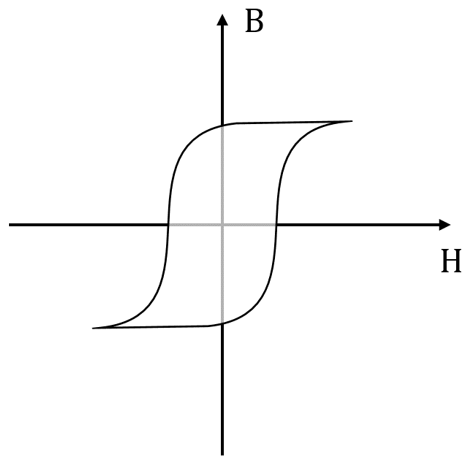
\includegraphics[width=0.40\textwidth]{chap2/images/large_bh_loop.png}
                \label{fig:chapter/background/bh loop/large}
            }
            \qquad
            \subfloat[]{
                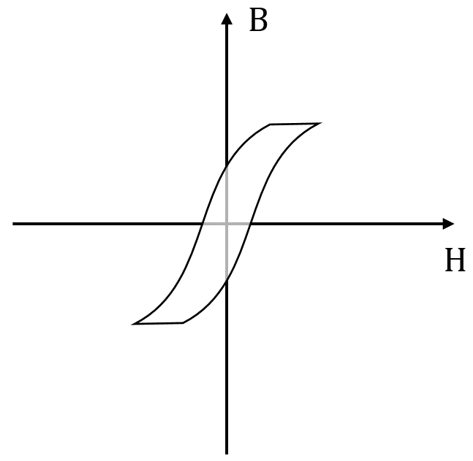
\includegraphics[width=0.4\textwidth]{chap2/images/narrow_bh_loop.png}
                \label{fig:chapter/background/bh loop/narrow}
            }
            \caption{
                Illustration of magnetic hysteresis for different ferromagnetic materials. Large $B-H$ curve (a) retains a significant fraction of magnetic flux density $B$ when the applied magnetic field $H$ is removed. Narrow $B-H$ curve (b) implies small energy dissipated when the applied magnetic field H is changing in the material.
            }   \label{fig:chapter/background/bh loop}
        \end{figure*}
        
        
        The gradient of the $B-H$ curve is the value of material permeability $\mu$. Ferromagnetic material with a linear $B-H$ relationship, or in other words, materials having the constant permeability over a range of applied H-fields, are relatively easier to model because losses caused by the changing of H-field can be predicted without the need of iterative numerical methods. There have been many successes with modelling Neodymium NdFeB rare-earth permanent magnets because this material has high $B_{rem}$, high $H_{ci}$, and $B-H$ linearity over a wide range of applied $H$-field. Iron, however, has a relatively low $B_{rem}$ and narrow range of $B-H$ curve linearity which makes it difficult to predict losses caused by magnetic hysteresis. Although a lookup table can be created, however, such a data table needs to include frequency in addition to the fields amplitude. 
        
        
        A wide hysteresis loop, as illustrated in Figure\,\ref{fig:chapter/background/bh loop/large} may seem ideal for permanent magnets because the material will likely retain a large fraction of magnetization field once the driving field is removed. However, for materials used as a magnetic conductor to close the effective air gap like iron, a narrow hysteresis loop is desired. A narrow hysteresis loop, as shown in Figure\,\ref{fig:chapter/background/bh loop/narrow} implies that only a small amount of energy is lost during repeated shifting of the magnetization which occurs every time the magnet moves relative to the iron. Hysteresis loss is still a tough effect to solve analytically.
        
        
        As mentioned above, in a magnetized ‘hard’ ferromagnetic material such as a permanent magnet, there exists a net magnetic moment without an applied external field $H$. The more convenient representation for a permanent magnet introduces $M_0$ as an additional magnetic moment term:


        \begin{equation}
            B = \mu_0 (H + M + M_0)
            \label{eq:B field equation 1}
        \end{equation}   
        
        \begin{equation}
            B = \mu_0 \mu_r H + \mu_0 M_0
            \label{eq:B field equation 2}
        \end{equation}   
        
        \begin{equation}
            M_0 = \frac{B_{rem}}{\mu_0}
            \label{eq:B rem equation}
        \end{equation}  
        
    
    % -----------------------------------------------------------------------------------
    % --- NEW SUB SECTION --- NEW SUB SECTION --- NEW SUB SECTION --- NEW SUB SECTION --- 
    % -----------------------------------------------------------------------------------
    \subsection{Force production}                   \label{Chapter:background/electromagnetic field theory/force production}
    
        Lorentz's force equation describes force $\overrightarrow{f}$ experienced by a charge $q$ moving with a velocity $\overrightarrow{v}$:
        
        
        \begin{equation}
            \overrightarrow{f} = q(\overrightarrow{E} + \overrightarrow{v} \times \overrightarrow{B})
            \label{eq:lorentz force equation}
        \end{equation}   
        
        
        where there is a electric field $\overrightarrow{E}$ and a magnetic field $\overrightarrow{B}$. The first part of the equation describes the force exerted on a charge by the mere presence of an electric field $\overrightarrow{E}$. The second part of the equation describes the force created when a moving charge is crossing a magnetic field $\overrightarrow{B}$. Force $\overrightarrow{F}$ is the resultant force acting on a body of given volume $V$ with current density $J$ flowing through volume $V$:
        
      
        \begin{equation}
            \overrightarrow{F} = \int_V \overrightarrow{J} \times \overrightarrow{B} \mathrm{d}v
            \label{eq:volume generalized lorentz}
        \end{equation} 
        
        
        Calculating the cross product of the free current density and the magnetic flux density requires knowledge of the total current density in the domain considered, i.e., the sum of all free and microscopic currents at an atomic level.
        Instead, to calculate the electromagnetic force acting on a body, we can perform surface integration of the Maxwell's stress tensor $\mathbb{T}$ around the body enclosed by surface area $S$ and an outward unit normal to the bounding surface $\overrightarrow{n}$:
        
        
        \begin{equation}
            \overrightarrow{F} = \oint_{S} \mathbb{T} \cdot \overrightarrow{n} \mathrm{d}s
            \label{eq:surface generalized lorentz}
        \end{equation}     


        % where the Maxwell's stress tensor, $\sigma$, consists of only the magnetic field component but not the electric field component, is coordinate system independent and defined as:


        % \begin{equation}
        %     \label{eq:maxwell stress tensor}
        %     \sigma_{ij} = \frac{B_i B_j}{\mu_0} - \delta_{ij} \frac{| \overrightarrow{B} |^{2}}{2\mu_0}
        % \end{equation}
                
        % \begin{equation}
        %     \notag
        %     \begin{split}
        %         \text{where Krocher delta} \quad \delta_{ij} =
        %             \begin{cases}
        %                 1       & \text{if $i=j$,}\\
        %                 0       & \text{if otherwise}
        %             \end{cases}
        %     \end{split}
        % \end{equation}
        

% ===================================================================================================
% === NEW SECTION === NEW SECTION === NEW SECTION === NEW SECTION === NEW SECTION === NEW SECTION ===
% ===================================================================================================
\section{Modelling techniques for motors}           \label{Chapter:background/modelling techniques for designing motors}


    Electric machines are devices that either produce force as a product of electric current and magnetic field, or harvest electric current from a conductor in contact with a changing magnetic field. It is necessary to estimate rated power, efficiency, and losses to optimize and achieve design goals. These estimations often require calculation to work out one or more machine characteristics using different forms of Maxwell's equations, governed by the relationship between constitutional materials, geometry, and configurations that apply to individual machines. Quasi-static or low-frequency assumption has been extensively used to model synchronous motors. Methods to solve quasi-static Maxwell's equations indirectly via either magnetic vector potential $A$ or scalar potential $\varphi$ are mentioned in Section\,\ref{Chapter:background/electromagnetic field theory/quasi-static maxwell equations}. The method for solving Maxwell's equations to model electric machines can fall under three categories: numerical, analytical or semi-analytical. Recently, motor types yet to be well understood can be modelled using empirical methods by collecting a vast amount of simulation data and fitting the motor variables and performance onto a set of non-linear equations.


    % -----------------------------------------------------------------------------------
    % --- NEW SUB SECTION --- NEW SUB SECTION --- NEW SUB SECTION --- NEW SUB SECTION --- 
    % -----------------------------------------------------------------------------------
    \subsection{Numerical methods}                  \label{Chapter:background/modelling techniques for designing motors/numerical methods}
    
    
        Mathematically speaking, Maxwell's equations are \acsp{PDE}. Numerical methods approximate the \acsp{PDE} into a system of linear equations by discretization of the spatial domain into smaller building blocks. These components are also called meshes, which are often triangular in the case of two-dimensional and tetrahedral for three-dimensional problems. Fine discretization, at the cost of an increase in computation effort, generally gives better results than coarse discretization. Boundary conditions will alter the set of governing equations appropriately. If discretization occurs throughout the body of the materials, this method is referred to as a \ac{FEM} or \ac{FEA}\,\cite{Boglietti2009EvolutionMachines,Huang2009}. In case the discretization happens only at the surface of the materials, it is referred to as a \ac{BEM}\,\cite{Fetter1998TransientCoil,Qaseer2014HybridMotor}. 
        
        \acs{FEA} is widely used because it can solve complex geometry, include nonlinear material properties and account for coupling between multiple types of physics (thermal, magnetic, mechanical) using nonlinear iterative algorithms\,\cite{Sizov2013AutomatedEvolution}. Out of the three categories, the numerical method requires the most computation effort. Often, \acs{FEA} requires too much computational effort to be used directly in optimization. Tuning for a single parameter may take several hours or days, depending on the mesh density. \acs{FEA} is usually used to evaluate the accuracy of analytical and semi-analytical models.

    
    % -----------------------------------------------------------------------------------
    % --- NEW SUB SECTION --- NEW SUB SECTION --- NEW SUB SECTION --- NEW SUB SECTION --- 
    % -----------------------------------------------------------------------------------
    \subsection{Analytical methods}                 \label{Chapter:background/modelling techniques for designing motors/analytical methods}
    
    
        The most commonly used analytical modeling method is known as \ac{MEC}. Similar to \acs{FEA}, the geometry is discretized. However, the number of elements is much smaller. Prior knowledge of flux distribution is necessary to construct an accurate model. Discretized flux tubes with assumed constant flux distribution are used to simplify the real problem. Instead of finding a direct solution for the Maxwell's equations, the flux distribution represented in terms of lumped flux tubes is modelled using electric circuit analogy. Magnetic flux is obtained as a product of given \ac{MMF} due to the magnetic field source.  
        
        
        \acs{MEC} takes a simple form and very low computational time. Saturation can be taken into account by splitting a soft magnetic object into multiple flux tubes with permanence dependent upon the magnetic field strength through each tube. Effects such as flux leakage and fringing are difficult to take into account because this approach assumes flux enters and leaves solely in the axial direction of the flux tubes. The differences in relative permeability between the regions are usually not taken into account, and relative permeability for air is assumed as unity. For the stated reasons, \acs{MEC} performs poorly in structures with large air gaps or structures with no magnetic bridge (iron) at all\,\cite{DeBoeij2006}. 
        
        
        The exact analytical approach to modelling electromagnetic environment in the literature has obtained success with modelling the magnetic fields of permanent magnet\,\cite{Ravaud2010}. Other analytical methods include solving complex functions and Schwarz–Christoffel transformation\,\cite{Zarko2006}, and motor phase circuit modelling\,\cite{Proca2003}.
        
        
    % -----------------------------------------------------------------------------------
    % --- NEW SUB SECTION --- NEW SUB SECTION --- NEW SUB SECTION --- NEW SUB SECTION --- 
    % -----------------------------------------------------------------------------------
    \subsection{Semi-analytical methods}            \label{Chapter:background/modelling techniques for designing motors/semi-analytical methods}
    
    
        One of the most popular semi-analytical methods takes the form of \ac{HM}. This approach uses the harmonic series or Fourier series to express the magnetic field formulation in 2D and 3D, based on the theory of transfer relation\,\cite{Melcher1981}. The problem is divided into material regions whose boundaries are orthogonal with axes of the coordinate system. The magnetic potentials in the quasi-Halbach magnet array and poly phase winding can be described in terms of a Fourier series. In each region, the equations for vector or scalar magnetic potential can take the form of Laplace or Poisson equations in Cartesian coordinates\,\cite{Trumper1993,Wang1999}. In cylindrical coordinates, the equation for magnetic potential takes the form of the Bessel function\cite{Gysen2008,Ruddy2011a,Gysen2011a}. The most widely used method to solve for the magnetic potential is separation of variables method. The coefficients in magnetic flux density equations, made up of magnetic potential terms are obtained by applying the boundary equations. The magnetic field can then simply be found via the constitutive relationship with magnetic flux density.
        
        
        This modelling technique is excellent for periodic geometry as in long stroke linear machines. Since long stroke synchronous motors have repeating segments of the same structure, the analysis only needs to be limited to a single wavelength with periodic boundary conditions. The end effect is dealt with separately. \acs{HM} is capable of taking linear material properties into account although iron is often assumed to be infinitely permeable. Models which can account for saturation exist in form or diffusion equation or adopt an iterative method that calculates the magnetic field based on the nonlinear B-H curve. \acs{HM} can compute slower than \acs{MEC} but faster than \acs{FEM}. High accuracy and relatively good speed allow HM approaches to be used directly in multi-variable optimization. Different motor geometry configuration requires a different set of \acsp{PDE} to be solved in order to determine the general solution for the magnetic potential in each spatial region. This is a mathematically rigorous process. In validating solutions to the \acsp{PDE}, the tests are checking for continuity behaviour of underlying magnetic fields, and strong agreement with \acs{FEM} results.
        
        
        \ac{MCM} is an alternative method resulting from the use of Green’s integrals to solve Maxwell's equations. Volume integrals are used to obtain magnetic scalar potential under the assumption that the materials used are current free. It is not possible to model the magnetic field due to current using the scalar potential, and thus reduced scalar potential\,\cite{Gong2009} is introduced for this purpose. The reduced scalar potential is robust and convenient for calculating eddy loss in soft ferromagnetic materials\,\cite{Xu2004,Bowler1987,Rubinacci2004}. Magnetization in permanent magnets is replaced by equivalent surface and volume magnetic charge terms with unit permeability. Only constant permeability on the whole domain is considered. \acs{MCM} has not achieved the level of accuracy that \acs{HM} has.
        
    
    % -----------------------------------------------------------------------------------
    % --- NEW SUB SECTION --- NEW SUB SECTION --- NEW SUB SECTION --- NEW SUB SECTION --- 
    % -----------------------------------------------------------------------------------
    \subsection{Empirical methods}                  \label{Chapter:background/modelling techniques for designing motors/empirical methods}


        Due to the complex flux path in motor typologies such as Flux Switching Motors and Transverse Flux Motors, reflected by the difficulty in semi-analytical modelling for this type of motor, the literature typically makes use of $\mathrm{2D}$ or $\mathrm{3D}$ \acs{FEA} to accurately predict the thrust and cogging force. Traditionally, during the optimization process, each performance valuation requires one FEM evaluation. This means the simulation is only needed once. Thus, this approach is considered having poor data re-use, and unpredictable optimization wait time. Instead, we can approach motor design with the \acf{RSM}, by describing the motor performance metrics using empirical equations\,\cite{Hong2008,Lei2013}, or using an artificial neural network\,\cite{Hadjout2006,Ashabani2010}. Once an arithmetic model is fitted to represent the data set, model inference time is a number of magnitudes lower than the simulation time for each valuation. A high number of recent motor design and control research has obtained various degree of success with this approach\,\cite{Hwang2007,Lee2012,Kim2006,Jung2015,Hong2018}. 
        
        
        In a high order \acs{RSM} problem with many input variables, high sampling levels for each input are the key to obtaining accurate model predictions. However, the time and computation effort required are growing exponentially with each additional parameter and sampling level for existing parameter. Planning and execution of \acs{RSM} is in this sense a data exploratory exercise. It is difficult to predict what range of data is needed ahead of time.


% ===================================================================================================
% === NEW SECTION === NEW SECTION === NEW SECTION === NEW SECTION === NEW SECTION === NEW SECTION ===
% ===================================================================================================
\section{Optimization methods}                      \label{Chapter:background/optimization methods}
    
    
    Mathematical optimization techniques offer a methodical way of approaching design problems. Optimization is commonly performed by minimizing cost functions and can be applied to a wide variety of applications:
    
        
    \begin{equation}
        \begin{array}{rll}
            \textbf{minimize}       & \small{objective\,\,function}         & f(x)\\ 
            \textbf{subject to}     & \small{inequality\,\,constraints}     & g_i(x) \leqslant 0, \text{for } i= 1,...,m,\\ 
                                    & \small{equality\,\,constraints}       & h_i(x) = 0, \text{for } j= 1,...,n,\\ 
                                    & \small{variable\,\,space}             & x \in X
        \end{array}
    \end{equation}
    
    
    An alternative is the direct grid search or exhaustive search, in many cases attempt to consider the complete design space. By mapping the performance of every single machine design in a discretized variables to a performance index value, this method can help identify a Pareto front of designs in which the performance could not be further improved. The most suitable machine can then be selected from the group of Pareto-optimum designs, based on the specific requirements and trade-offs of the application.
    
    
    % -----------------------------------------------------------------------------------
    % --- NEW SUB SECTION --- NEW SUB SECTION --- NEW SUB SECTION --- NEW SUB SECTION --- 
    % -----------------------------------------------------------------------------------
    \subsection{Optimization problem classification}    \label{Chapter:background/optimization methods/optimization prob classification}

        
        Some problems only allow variables to take on discrete values, often a subset of integers, whereas other variables can be any real values. Therefore, optimization problems can be classified based on the nature of the variables:

        \begin{itemize}
            \item Discrete optimization - all variables take the form of discrete or boolean values,
            \item Continuous optimization - all variables are continuous
            \item Mixed-integer optimization - some variables in the are discrete while others take continuous values
        \end{itemize}
   
        Another distinction to have is whether the problem is constrained or not. The constraint may be as simple as being bound to the input variable of the objective function to be minimized, or more complex like explicit equal or greater than equal relationships among the variables. Unconstrained optimization problems arise directly from a limited set of applications. In the case of motor design, there often exist limitations such as a desired weight or length or tolerable cogging force.
        
        
        Most optimization problems will have a single objective function to be minimized. However, there are multi-objective problems where people are more interested in the trade-off between the objectives function instead of finding a single satisfactory design. For instance, the problem requires the lightest motor while maximizing force output. In practice, multi-objective problems with multiple objectives will be rearranged as a single objective problem by replacing some objectives as constraints, or by creating a new objective function such as a weighted combination of the original objective functions.
        

    % -----------------------------------------------------------------------------------
    % --- NEW SUB SECTION --- NEW SUB SECTION --- NEW SUB SECTION --- NEW SUB SECTION --- 
    % -----------------------------------------------------------------------------------
    \subsection{Optimization in motor design}        \label{Chapter:background/optimization methods/optimization in motor design}
    
    
        The increase in speed and reduction in price of computer hardware, together with the development of faster algorithms as well as highly accurate \acs{FEA} models allow theoretical optimum design to be obtained. The design of permanent magnet motors or actuators has been discussed in many textbooks; however, a standard method does not exist since the application together with different sets of applicable constraints determines the strategy. The design of \acsp{PMLSM} for \acs{NFJI} is no exception. Ideally, the actuator should have high force density and the energy losses should be minimal. 
    
        
        One class of optimization methods is a group of gradient methods, in which the search direction is determined by the local gradient of the objective function at the current search point. Such algorithms are referred to as non-linear programming. Though straight forward to implement, these algorithms tends to converge to local optimum. If the problem at hand is a mixed integer optimization problem, the discrete variables will be treated separately by considering all possible combinations of the discrete variables as separate optimization problems\,\cite{Ruddy2015a}. This class of optimization algorithm has been demonstrated to be working well with semi-analytical and analytical modeling techniques\,\cite{Overboom2010,Aleksandrov2018,Fang2008}. 
        
        
        The other class of optimization algorithm is evolutionary methods. They are probability based algorithms which start with an initial population of design candidates and simulate a breeding environment. The characteristics of each design are used to generate a fitness value to indicate its level of performance with respect to other designs in the population. After each generation, breeding is carried out to combine the characteristics of selected parent designs with the hope of yielding a better next generation of designs. This class of algorithm has the capacity to handle both discrete and continuous variables. The random mutation guarantees to some extent that we see a wide range of solutions. However, it is rather tricky to choose parameters such as the number of generation, the population and the mutation probability. Despite the experiment-like nature of this class of methods, the literature has applied this method extensively in motor design, starting from proven analytical and semi-analytical models\,\cite{Isfahani2007,Li2014,Mallik2017,RuiHuang2008}.
        
        
        Direct use of \acs{FEM} is far less suitable for optimization purposes due to the long computation time taken to evaluate a single objective function. Even with simple structures, the creation of mesh can be the most time-consuming task. One way to overcome this limitation is to replace the online \acs{FEM} function evaluation with a simplified function that requires far less time to compute. As mentioned in Section\,\ref{Chapter:background/modelling techniques for designing motors/empirical methods}, these methods are classified as empirical modelling methods. Once there exists a simplified model to represent the design space, gradients and evolutionary methods can be applied to find the globally optimal motor design\,\cite{Ashabani2010,Lee2012,Giurgea2007,Hasanien2010, Hasanien2011,Zhang2017}. 

    \chapter{\acsp{LSDDM} design with Harmonics Modelling}   \label{Chapter:PMLSM design HM}


    From the previous chapter, it was pointed out that the scaling laws for \acfp{PMLSM} allow the overall \acf{NFJI} system to operate at a much higher efficiency when compared to \acf{VCM}. \acsp{PMLSM} or more precisely tubular, slotless, permanent magnet excited, longitudinal flux, and linear 3-phase motors have shown superior potential when compared to \acsp{VCM} in \acs{NFJI} applications\,\cite{Ruddy2015}. This chapter considers the requirements tailored to \acsp{NFJI} to describe a modified design of the present \acs{PMLSM} . 


    The potential of a better actuator for \acs{NFJI} has been proven with \acsp{PMLSM}, accompanied with computationally efficient, exact semi-analytical magnetic field \acf{HM} solutions. However, a large efficiency gain is only possible if the total length of the motor is allowed to be very long which will be impractical for fitting into an actual injector device. An appropriate optimization scheme with the necessary constraints will be required to not only realize a practical actuator for an \acs{NFJI} but be flexible enough to compare with other types of \acsp{LSDDM} in existence. To address this challenge, an universal optimization scheme for \acsp{LSDDM} with fixed maximum motor length, motor mass, and input power dissipation is required. This optimization method helps determine a \acs{PMLSM} motor design that will produce the fastest water jet injection velocity with the given constraints. 


% ===================================================================================================
% === NEW SECTION === NEW SECTION === NEW SECTION === NEW SECTION === NEW SECTION === NEW SECTION ===
% ===================================================================================================
\section{Electromagnetic model}                 \label{Chapter:PMLSM design HM/electromagnetic model}


    % -----------------------------------------------------------------------------------
    % --- NEW SUB SECTION --- NEW SUB SECTION --- NEW SUB SECTION --- NEW SUB SECTION --- 
    % -----------------------------------------------------------------------------------
    \subsection{Scaling model}                  \label{Chapter:PMLSM design HM/electromagnetic model/scaling}


        \begin{figure*}[ht]
          \centering
          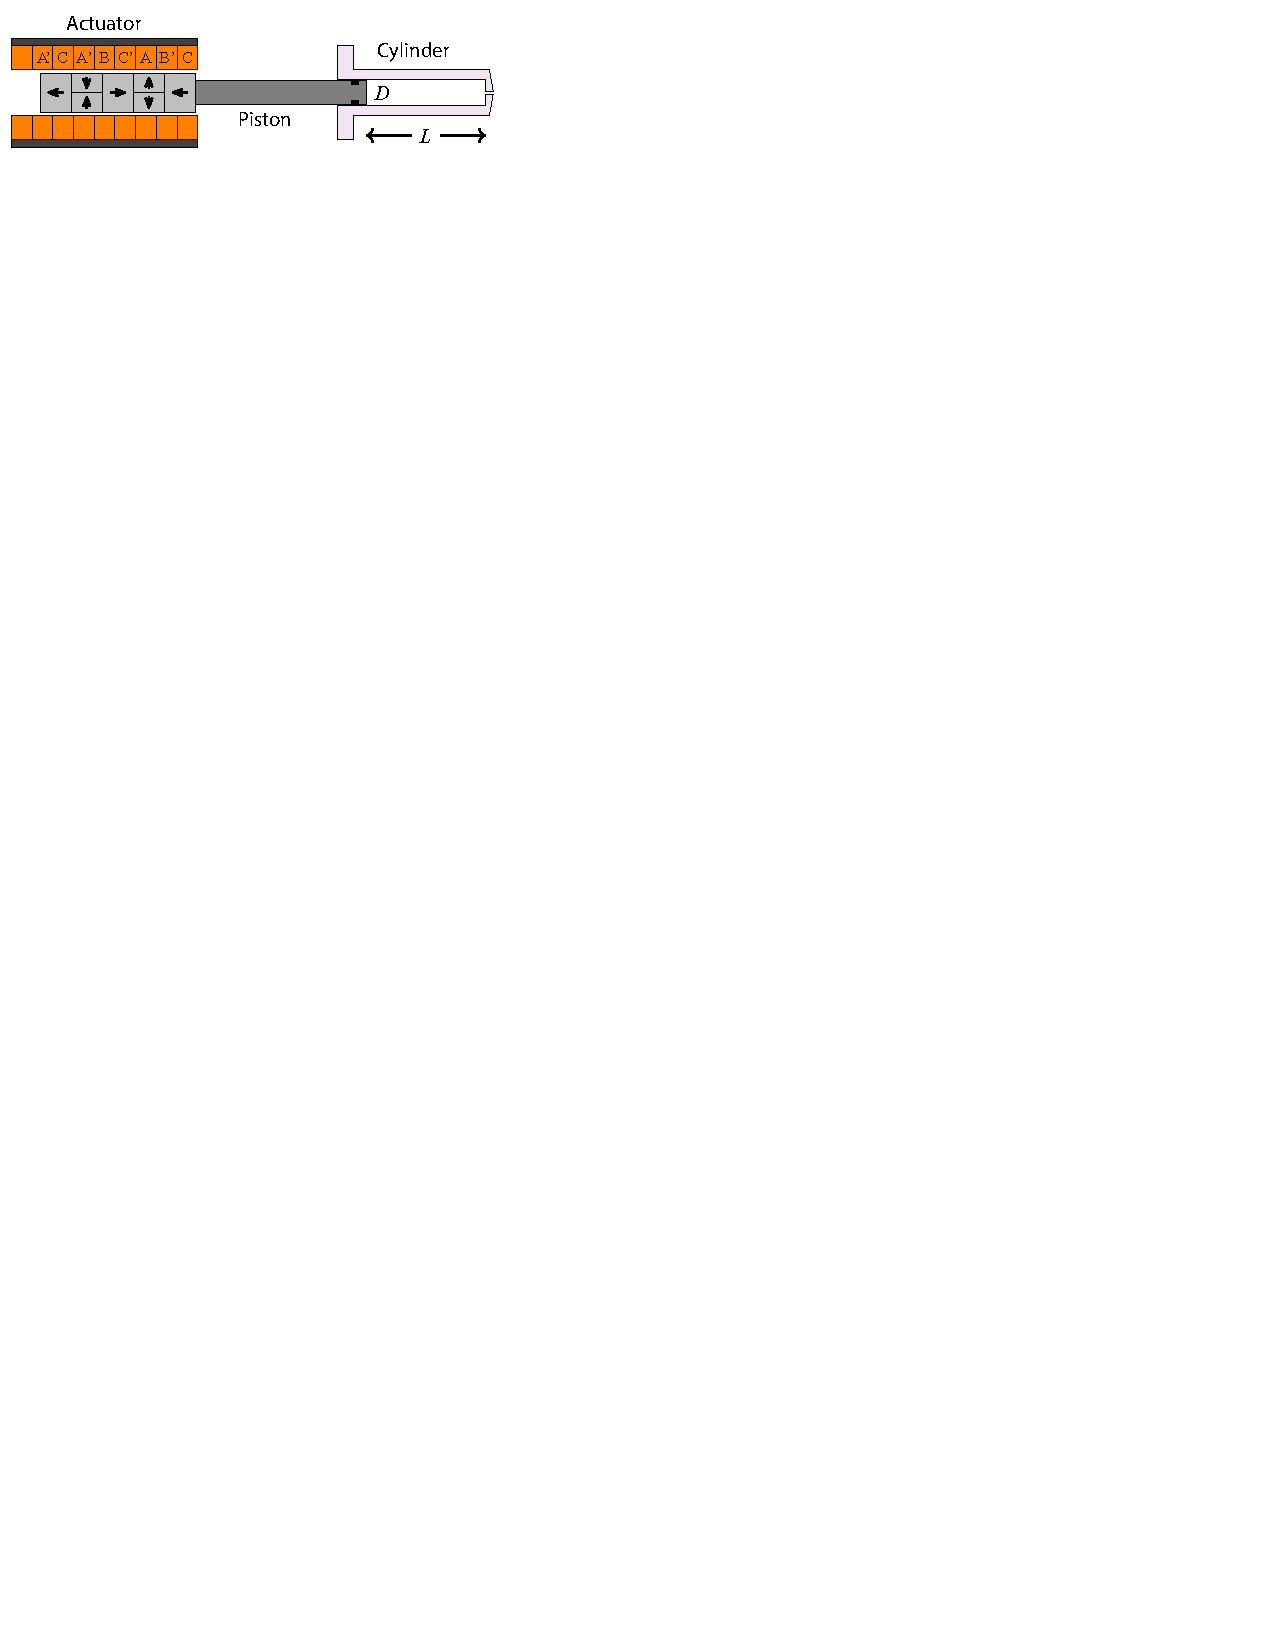
\includegraphics[width=0.7\textwidth]{chap3/images/PMLSM_scaling_law_illustration.pdf}
          \caption[A basic schematic of a synchronous motor, driving a jet injector. Ampoule diameter $D$ and piston stroke $L$ are illustrated.]{A basic schematic of a synchronous motor, driving a jet injector. Ampoule diameter $D$ and piston stroke $L$ are illustrated\,\cite{Ruddy2015}.}
          \label{fig:chapter/hm/PMLSM scaling law illustrated}
        \end{figure*}


        Ignoring resistance due to fluid viscosity, due to Bernoulli's equation for an incompressible and steady fluid flow, the actuator force $F$ and jet speed $v_{jet}$ have the following relationship:
        
        
        \begin{equation}
            F=\frac{\pi}{8}\rho_w {v_{jet}}^2 D^2
            \label{eq:actuation force by PMLSMs}
        \end{equation}
        
        
        where $\rho_w$ is the density of fluid being delivered and $D$ is the diameter of the piston cylinder. For linear permanent magnet motors, the motor constant $K_m$, measured in $\mathrm{N/\sqrt{W}}$, is a measurement of force production efficiency that is independent of the winding properties. We can combine these relationships to find the power dissipation in the motor windings $P$ for a given ampoule volume $V$ and length of piston travel $L_s$:


        \begin{equation}
            P=\frac{\rho^2V^2{v_{jet}}^4}{4{K_m}^2 L_s^2}
            \label{eq:power dissipation for PMLSMs}
        \end{equation}
        
        
        It was shown in \cite{Ruddy2011a} that $K_m \propto {\hat K}_m \sqrt M$, where ${\hat K}_m$ is a dimensionless parameter describing the internal magnetic and electric geometry of the motor. Thus, neglecting material properties, we can determine the overall scaling behavior of motors for the needle free jet injection task:
        
        
        \begin{equation}
            P\propto\frac{V^2v^4}{ {M L_s^2{\hat K^2}_m} }
            \label{eq:scaling law for PMLSMs}
        \end{equation}
        
        
        Typically the application determines $\rho$, $V$, $v$, and $L_s$ (or $D$). Thus, either motor mass $M$ must be fixed to search for a motor with the optimum power consumption $P$, or $P$ must be fixed to find a motor with the minimum motor mass.


    % -----------------------------------------------------------------------------------
    % --- NEW SUB SECTION --- NEW SUB SECTION --- NEW SUB SECTION --- NEW SUB SECTION --- 
    % -----------------------------------------------------------------------------------
    \subsection{Topology}                       \label{Chapter:PMLSM design HM/electromagnetic model/topology}
    
    
        \begin{figure*}[ht]
          \centering
          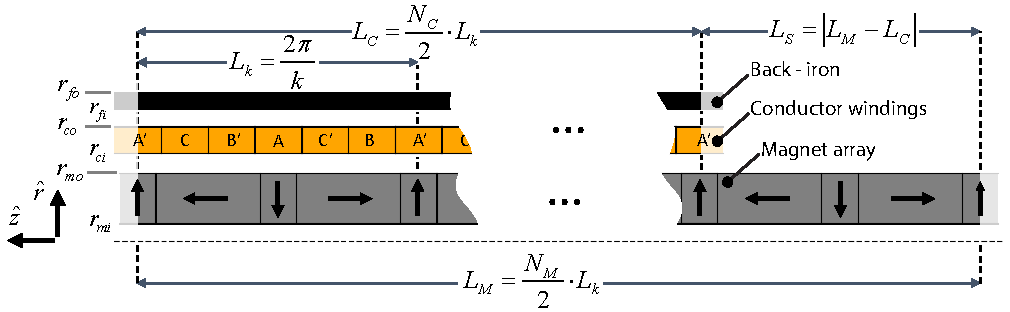
\includegraphics[width=5.8in]{chap3/images/PMLSM.pdf}
          \caption{This schematic illustrates a tubular LPMSM with quasi-Halbach magnets, slotless windings, and a shortened exterior back-iron tube. The radii of magnet, coil, and back are shown; the structure has periodicity with wave number $k$, wave length $L_k$, number of half coil poles $N_C$ and half magnet poles $N_M$. The arrows indicate the direction of magnetization of the magnets, while the characters label the coil phases.}
          \label{fig:chapter/hm/PMLSM motor construction fullpage}
        \end{figure*}
    
        
        Based on \cite{ruddy2014}, we will study a slight variation of this topology using a shorter exterior back-iron. In this approach, the back-iron only covers the coil and travels along with it, as shown in Fig.~\ref{fig:chapter/hm/PMLSM motor construction fullpage}. The advantage of the shortened back-iron over using iron to cover the entire motor length is the reduction in weight, which is an important objective in designing handheld devices. However, a moving-iron configuration introduces cogging effects that can be problematic for smooth motion control.
        
        
        We analyzed a motor with repeat units of coil and magnet of wavelength $L_k$, ratio of radial magnet length over a pair of radial-axial magnet $\delta$, coil length $L_C$, magnet length $L_M$, and arbitrary number of half coil poles  $N_C$ and magnet poles $N_M$, as illustrated in Fig.~\ref{fig:chapter/hm/PMLSM motor construction fullpage}. The motor is overhung if $N_C>N_M$, and underhung if $N_M>N_C$. Previous research in \cite{Ruddy2015} points out that underhung motors offer superior efficiency to overhung motors; thus, only underhung motors are considered here. The length of the motor simplifies to:
        
        
        \begin{equation}
            L_{motor}\equiv L_M=\frac{N_M}2\cdot L_k
            \label{eq:PMLSMs motor length}
        \end{equation}
        
    
    % -----------------------------------------------------------------------------------
    % --- NEW SUB SECTION --- NEW SUB SECTION --- NEW SUB SECTION --- NEW SUB SECTION --- 
    % -----------------------------------------------------------------------------------
    \subsection{Harmonic modelling solution}               \label{Chapter:PMLSM design HM/electromagnetic model/hm solution}

                
        Our modeling approach is outlined in \cite{Ruddy2011a} and employed in \cite{ruddy2014,Ruddy2015}. An analytical Fourier series solution was used to solve Poisson's equation in cylindrical coordinates directly. This formulation provides a good tradeoff between accuracy and computational efficiency. It computes faster compared to FEA \cite{Jin2014} or the standard integral formulation \cite{Wang1999,Bianchi2000} and avoids the problems of numerical instability exhibited by other explicit analytical solutions \cite{Wijono2010,Yan2013}.
        
        
        Uniformly magnetized segments are used in place of each radial magnet to approximate true radial magnetization. The magnetization of permanent magnets can be represented by a Fourier series where ${\hat M}_{rn}$ and  ${\hat M}_{zn}$ are the dimensionless radial and axial magnetizations, respectively:


        \begin{equation}
            {\hat M}_{rn}=\frac{4N_{seg}}{n\mathrm\pi^2}\sin\left(\frac{\mathrm\pi}{N_{seg}}\right)\sin\left(\frac{n\pi\delta}2\right)
            \label{eq:Mrn}
        \end{equation}
        
        
        \begin{equation}
            {\hat M}_{zn}=-\frac4{n\mathrm\pi^2}\cos\left(\frac{n\pi\delta}2\right)
            \label{eq:Mzn}
        \end{equation}
        
        
        in odd harmonic order $n$, the number of uniformly magnetized segments used to approximate true radial magnetization $N_{seg}$, and the fraction of magnet array occupied by radial-orientated magnets $\delta$. This imperfection is also accounted for in the model by a method of analyzing 3D effects in a segmented Halbach array \cite{Meessen2011}.


        Valid for an idealized back-iron with constant permeability, the solutions to Maxwell's equations for this set of boundary conditions can be described in terms of auxiliary functions ${\mathrm\Lambda}_{\nu}$ based on the modified Struve function ${\mathrm{L}_{\nu}}(x)$, and the modified Bessel functions ${\mathrm I}_{\nu}(x)$, and ${\mathrm K}_{\nu}(x)$:
        
        
        \begin{equation}
            {\Lambda_{\nu}}\left( x \right) \equiv \frac{\pi }{2}\left( {{\mathrm{I}_{\nu}}\left( x \right) - {\mathrm{L}_{\nu}}\left( x \right)} \right)
            \label{eq:Axiliary function}
        \end{equation}
        
        \begin{equation}
            {\mathcal{L}_{{\textrm{ I}}}} \equiv x\left( {{\Lambda _1}\left( x \right){\mathrm{I}_0}\left( x \right) - {\Lambda _0}\left( x \right){\mathrm{I}_1}\left( x \right)} \right)
            \label{eq:bessel function 1}
        \end{equation}
        
        \begin{equation}
            {\mathcal{L}_{{\textrm{ K}}}} \equiv x\left( {{\Lambda _1}\left( x \right){\mathrm{K}_0}\left( x \right) + {\Lambda _0}\left( x \right){\mathrm{K}_1}\left( x \right)} \right)
            \label{eq:bessel function 2}
        \end{equation}
        
        
        The force $F$ can be found by determining a dimensionless force constant $\hat F$. We compute $\hat F$ by integrating the Lorentz force over the coil:
        
        
        \begin{equation}
            \hat{F}=\mathrm\pi\left({\hat{a}}_{1c}{\hat{b}}_{1m}+{\hat{a}}_{1m}{\hat{b}}_{1c}\right)
            \label{eq:force dimless}
        \end{equation}
        
        
        where ${\hat a}_{1m}$ and ${\hat b}_{1m}$ are the magnetic field coefficients governed by matching boundary conditions for the first harmonic, and ${\hat a}_{1c}$ and ${\hat b}_{1c}$ are parameters controlled by the coil radii: 
        
        
        \begin{equation}
            \hat{a}_{1c}=\mathcal{L}_{\textrm{ K}}(k\,r_{co})-\mathcal{L}_{\textrm{ K}}(k\,r_{ci})
            \label{eq:a hat 1c}
        \end{equation}
        
        
        \begin{equation}
            \hat{b}_{1c}=\mathcal{L}_{\textrm{ I}}(k\,r_{co})-\mathcal{L}_{\textrm{ K}}(k\,r_{ci})
            \label{eq:b hat 1c}
        \end{equation}
        
        
        The force $F$ can then be obtained from the dimensionless force constant:
        
        
        \begin{equation}
            F = \frac{{2\pi {B_{rem}}{J_1}{N_M}}}{{{k^3}}}\hat F
            \label{eq:actual force}
        \end{equation}
        
        
        where $J_1$ is the magnitude of the first harmonic of current density, and $B_{rem}$ is the remanent magnetization of the permanent magnet. In a similar manner, power dissipation $P$ and motor mass $M$ can also be non-dimensionalized: 
        
        
        \begin{equation}
            \hat P = \frac{\pi }{2}\left[ {\,{{\left( {k{r_{ci}}} \right)}^2} - {{\left( {k{r_{co}}} \right)}^2}} \right]
            \label{eq:P dimless}
        \end{equation}
        
        
        \begin{equation}
            P = \frac{{2\pi {N_M}J_1^2}}{{\sigma {k^3}}}\hat P
            \label{eq:power via power dimless}
        \end{equation}
        
        
        \begin{equation}
            M = \frac{{2\pi {N_M}{\sigma _c}}}{{{k^3}}}\hat M
            \label{eq:mass of motor via mass dimless}
        \end{equation}
        
        
        \begin{equation}
            M = {M_{coil}} + {M_{magnet}} + {M_{iron}}
            \label{eq:sum of all mass}
        \end{equation}
        
        
        \begin{align*}
            \hat M = \pi \left[ {f + \left( {1 - f} \right)\frac{{{\rho _{ins}}}}{{{\rho _c}}}} \right]\left[ { {{\left( {k{r_{co}}} \right)}^2} - {{\left( {k{r_{ci}}} \right)}^2}} \right]\left( {\frac{{{N_C}}}{{{N_M}}}} \right)
            \\
            +  \pi \left( {\frac{{{\rho _m}}}{{{\rho _c}}}} \right)\left[ {\,{{\left( {k{r_{mo}}} \right)}^2} - {{\left( {k{r_{mi}}} \right)}^2}} \right]\qquad\qquad\qquad\quad
            \end{align*}
            \begin{equation}
            +  \pi \left( {\frac{{{\rho _f}}}{{{\rho _c}}}} \right)\left[ {\,{{\left( {k{r_{fo}}} \right)}^2} - {{\left( {k{r_{fi}}} \right)}^2}} \right]\left( {\frac{{{N_C}}}{{{N_M}}}} \right)\quad \,
            \label{eq:sum of all mass dimless}
        \end{equation}
        
        
        where $f$ is copper volume fill factor, $\rho_{ins}$ is the insulator density, $\rho_c$ is the conductor density, $\rho_m$ is magnet volumetric density, and $\rho_f$ is the iron density. Note that in the description of the dimensionless mass\,$\hat M$ the length of the back-iron follows the length of the coil. However, back-iron length will need to be adjusted to minimize end cogging effects, which will slightly increase the total mass. 
        
        
        The field solution for infinitely-permeable back iron has been derived previously\,\cite{ruddy2014} for any harmonic model $n$:


        \begin{equation}
            b_{nm}=\hat{M}_{r1}\Big(\mathcal{L}_{\mathrm{I}}(nkr_{mo})
            -\mathcal{L}_{\mathrm{I}}(nkr_{mi})\Big)-\hat{M}_{z1}\Big(nkr_{io}\mathrm{I}_1(nkr_{io})-nkr_{mi}\mathrm{I}_1(nkr_{mi})\Big)
            \label{eq:bnm}
        \end{equation}
        
        
        \begin{equation}
            a_{nm}=b_{nm}\frac{\mathrm{K}_0(nkr_{fi})}{\mathrm{I}_0(nkr_{fi})}
            \label{eq:anm}
        \end{equation}
        
        
        Ignoring the magnetic field produced by the applied current, the maximum flux density $B_{sat}$ can be found:
        

        \begin{equation}
            B_{sat}=\frac{r_{fi} B_{rem}}{{r_{fo}}^2-{r_{fi}}^2}\sum_{n=1}^\infty\frac{2\sin \left(\frac{n\pi}{2}\right)}{nk}\Big(a_{nm}\mathrm{I}_{1}(nkr_{fi})-b_{nm}\mathrm{K}_{1}(nkr_{fi})\Big)
            \label{eq:Bsat}
        \end{equation}
        
        
        With the field solution for an infinitely permeable back-iron $a_{nm}$, $b_{nm}$, and the maximum allowed flux density $B_{sat}$, the back-iron outer radii $r_{fo}$ can be constrained using the relationship:


        \begin{equation}
            r_{fo}=\sqrt{{r_{fi}}^2+r_{fi}\frac{B_{rem}}{B_{sat}}\sum_{n=1}^\infty{\frac{{2\sin ( {\frac{{n\pi }}{2}} )}}{{nk}}\Psi }}
            \label{eq:r_fo}
        \end{equation}
        
        \begin{equation}
            \Psi  = {a_{nm}}{{\textrm{I}}_{\textrm{1}}}\left( {nk{r_{fi}}} \right) + {b_{nm}}{{\textrm{K}}_{\textrm{1}}}\left( {nk{r_{fi}}} \right)
            \label{eq:psi}
        \end{equation}
        
        
        With $\sigma$ as the conductivity of the conductor, $w$ as the winding factor, and $N_{\phi}$ as the number of winding phases, the dimensionless motor constant ${\hat K}_m$ and the motor constant $K_m$ can be obtained via:


        \begin{equation}
            w = \frac{{2{N_\phi }}}{\pi }\sin \left( {\frac{\pi }{{2{N_\phi }}}} \right)
            \label{eq:winding factor}
        \end{equation}
        
        
        \begin{equation}
            {K_m} = {B_{rem}}{\hat K_m}\sqrt {\frac{{\sigma M}}{{{\rho _c}}}}
            \label{eq:K_m}
        \end{equation}
        
        
        \begin{equation}
            {\hat K_m} = w\hat F\sqrt {\frac{f}{{( {\frac{{{N_M}}}{{{N_C}}}} )\hat P\hat M}}}
            \label{eq:K_m dimless}
        \end{equation}
           
        
% ==============================================\propto{}=====================================================
% === NEW SECTION === NEW SECTION === NEW SECTION === NEW SECTION === NEW SECTION === NEW SECTION ===
% ===================================================================================================
\section{Benchmark study}                       \label{Chapter:PMLSM design HM/benchmark study}


    % -----------------------------------------------------------------------------------
    % --- NEW SUB SECTION --- NEW SUB SECTION --- NEW SUB SECTION --- NEW SUB SECTION --- 
    % -----------------------------------------------------------------------------------
    \subsection{Common design criteria}         \label{Chapter:PMLSM design HM/design optimization/design citeria}
    
    
        One of the main goal in this body of work is to be able to fairly compare different types of \acsp{LSDDM}. In order to achieve this goal, a common set of design criteria needs to be established as follows:
        
        
        \begin{itemize}
            \item The motor is powered by a single \acs{LSDDM}, regardless of which type,
            \item The device needs to deliver $1\,\mathrm{mL}$ of volume of fluid with a $200\,\mathrm{\mu m}$ nozzle outlet,
            \item The maximum power consumption allowed is $P=1500\,\mathrm{W}$,
            \item The benchmark weights for the motor optimization will be $325\,\mathrm{g}$, $350\,\mathrm{g}$, $375\,\mathrm{g}$, $400\,\mathrm{g}$, and $425\,\mathrm{g}$,
            \item The total length of the motor will be between $120\,\mathrm{mm}$ and $160\,\mathrm{mm}$,
            \item The total length of all coil phases ($N_C=1,2,3...$) will be between between $50\,\mathrm{mm}$ and $90\,\mathrm{mm}$.
        \end{itemize}
        
        
        The target volume $1\mathrm{mL}$ is standard to many macro-molecule drug formulations\,\cite{Hogan2015a}. Between $325\,\mathrm{g}$ and $425\,\mathrm{g}$ in weight is the ideal range for a comfortable handheld device. The power level is decided to be within the capability of practical self-contained power sources such as Panasonic Industrial's $\mathrm{	MDDHT5540E}$ or Omron Automation' $\mathrm{3G3MX2-A4015-V1}$. As mentioned in Section\,\ref{Chapter:background/needle-free jet injection/how it works}, the jet minimum jet speed required to puncture the skin is $100\,\mathrm{m/s}$. 
        
        
        This set of common design criteria will allow for a common optimization scheme that attempts to find the motor configuration with the highest achievable jet velocity across different types of \acsp{LSDDM}. The following content in this chapter and Chapter\,\ref{Chapter:PMLSM design RSM} will demonstrate that the implementation for each type of \acsp{LSDDM} studied by this thesis has to be adapted to the motor's unique characteristic.
        

    % -----------------------------------------------------------------------------------
    % --- NEW SUB SECTION --- NEW SUB SECTION --- NEW SUB SECTION --- NEW SUB SECTION --- 
    % -----------------------------------------------------------------------------------
    \subsection{Optimization formulation}       \label{Chapter:PMLSM design HM/design optimization/optimization formulation}
    
        \subsubsection{Outer optimization}      \label{Chapter:PMLSM design HM/design optimization/optimization formulation/out}
        
        
            The overall optimization consist of strategic repetition of the inner optimization to maximize the achievable jet speed $v_{jet}$:
        
        
            \begin{equation}
                \begin{array}{rll}
                    \textbf{minimize}       & \small{objective\,\,function}     & f(\textbf{x})=\frac{1}{v_{jet}} \\
                    \textbf{subjected to}   & \small{equality\,\,constraint}    & h_1(\textbf{x})=M - M_0= 0\\
                                            &\quad \small{where}                &\quad  M_0\in\left[325,350,375,400,425\right]\,\mathrm{g}\\
                                            &                                   & h_2(\textbf{x})=P - 1500\,\mathrm{W}=0\\
                                            &                                   & h_3(\textbf{x})=L_C - L_{C0} = 0\\
                                            &\quad \small{where}                &\quad  L_{C0}\in\left[50,51,52,...,90\right]\,\mathrm{mm}\\
                                            &                                   & h_4(\textbf{x})=V - 1\,\mathrm{mL} = 0\\
                                            & \small{inequality\,\,constraint}  & g_1(\textbf{x})=(L_S+L_C)-L_{M0} \leqslant 0\\
                                            &\quad \small{where}                &\quad L_{M0} \in \left[120,121,122,...,160\right]\,\mathrm{mm} \\
                                            & \small{other\,\,constraint}       & N_C, N_M \in 	\mathbb{N} \\ \\
                \end{array}
                \label{eq:outer optimization for PMLSMs}
            \end{equation}
            
            
            To get a realistic model, material properties, design constants and value ranges were introduced. A fill factor of $w = 62\,\%$ was assumed for the three-phase ($N_{\phi}=3$) copper conductor, and $1080$ carbon steel for the back iron shell. The radial magnet is approximated by 4 equal segments ($N_{seg}=4$ ). The saturation field is $B_{sat}=2\,\mathrm{T}$. All calculations were conducted up to $n \leq 11$ harmonics. Recalling the characteristics of \acsp{PMLSM}: each repeat length $L_{k}$ consists of 2 equal half-coil-phases $N_C$, as well as 2 half-magnet-phases $N_M$. 
            
            
            Figure\,\ref{fig:chapter/hm/PMLSM motor construction fullpage} shows that each half-coil-phase $N_C$ consists of three equally spaced windings. Naturally, each coil winding should be structurally sound with the minimum width per coil winding of $3\,\mathrm{mm}$, thus, the minimum value of $L_k$ is $18\,\mathrm{mm}$. The magnet array should be hollow to allow for reinforcement to be installed from one end to another end of the motor. The clearance between the magnet and coil $g_{mc}$ was set to $1.2\,\mathrm{mm}$ to facilitate for the rigidity of the moving structure that supports the coils. Additionally, the gap between the coil assembly and the outer iron shell $gap_{cf}$ is set to $0.1\,\mathrm{mm}$ for the ease of assembly. Both the coil thickness $t_c = r_{co}-r_{ci}$ and magnet thickness $t_m = r_{mo}-r_{mi}$ are set to be thicker than $3\,\mathrm{mm}$, respectively. Table\,\ref{table:table_of_optimization_constraints_PMLSM} summarizes the constraints on the desired motor configuration.
            
            
            \begin{table}
            \renewcommand{\arraystretch}{1.2}
            \caption{Summary of motor optimization constants and constraints of PMLSM}
            \label{table:table_of_optimization_constraints_PMLSM}
            \centering
            \begin{tabular}{llr}
                \hline
                \bfseries Parameters & \bfseries Description & \bfseries Values \\
                \hline
                    $t_c$	        & Coil thickness $t_c = r_{co}-r_{ci}$	    &	$\geq3\,\mathrm{mm}$\\ 
                    $t_m$	        & Magnet thickness $t_m = r_{mo}-r_{mi}$    &	$\geq3\,\mathrm{mm}$\\
                    $r_{mi}$		& Magnet array inner radius 			    &	$\geq2\,\mathrm{mm}$\\ 
                    $gap_{mc}$		& Magnet and coil fixed gap $gap_{mc}=r_{ci}-r_{mo}$    &	$1.2\,\mathrm{mm}$\\ 
                    $gap_{cf}$		& Coil and iron fixed gap $gap_{cf}=r_{fi}-r_{co}$ 	    &	$0.1\,\mathrm{mm}$\\ 
                    $L_k$			& Period length	 						    &	$L_{C} \geq L_k \geq 18\,\mathrm{mm}$\\
                    $\delta$		& Ratio of radial magnet over a period	    & 	$1> \delta >0$\\
                \hline
            \end{tabular}
            \end{table}
            
            
            Given each combination of $L_{C0}$ and $L_{M0}$, a set of $N_C$ and $L_k$ can be determined with the following relationship:
            
            
            \begin{equation}
                N_C \in \Bigg[\bigg\lceil {\frac{L_{C0}}{\mathrm{Max}(L_k/2)}} \bigg\rceil:\bigg\lfloor{\frac{L_{C0}}{\mathrm{Min}(L_k/2)}}\bigg\rfloor\Bigg] \equiv \Bigg[2:\bigg\lfloor{\frac{L_{C0}}{9\,\mathrm{mm}}}\bigg\rfloor\Bigg]
                \label{eq:list of NC}
            \end{equation}
            
            
            \begin{equation}
                L_k \in 2\frac{L_{C0}}{\left[N_C\right]}
                \label{eq:list of L_k}
            \end{equation}
        
        
            As the result, the total length of coil winding $L_C$ is always as long as $L_{C0}$, consistent with the $h_3$ relationship from Equation\,\ref{eq:outer optimization for PMLSMs}:
            
            
            \begin{equation}
                L_C = L_{C0} = N_C \frac{L_k}{2}
                \label{eq:L_C and L_C0}
            \end{equation}
            
            
            The aim is to make sure the number of half-coil-phase $N_C$ and half-magnet-phase $N_M$ are simultaneously a natural number, as well as maximizing the total length of motor $L_{M0}$ allowed ($g_1$ relationship from Equation\,\ref{eq:outer optimization for PMLSMs}). When choosing a particular $N_C$ and accompanying $L_C$ from the value sets worked out above, the stroke lengths $L_S$ and $N_M$ satisfy the following:
            
            
            \begin{equation}
                L_S = \bigg\lfloor L_{M0}\frac{ N_C}{L_C} \bigg\rfloor \frac{L_C}{N_C}-L_C
                \label{eq:L_S}
            \end{equation}
            
            
            \begin{equation}
                N_M = \frac{(L_S+L_C)}{\frac{L_k}{2}}
                \label{eq:N_M}
            \end{equation}
            
            
        \subsubsection{Inner optimization}      \label{Chapter:PMLSM design HM/design optimization/optimization formulation/inner}
            
            
                
            \begin{figure*}[h]
              \centering
              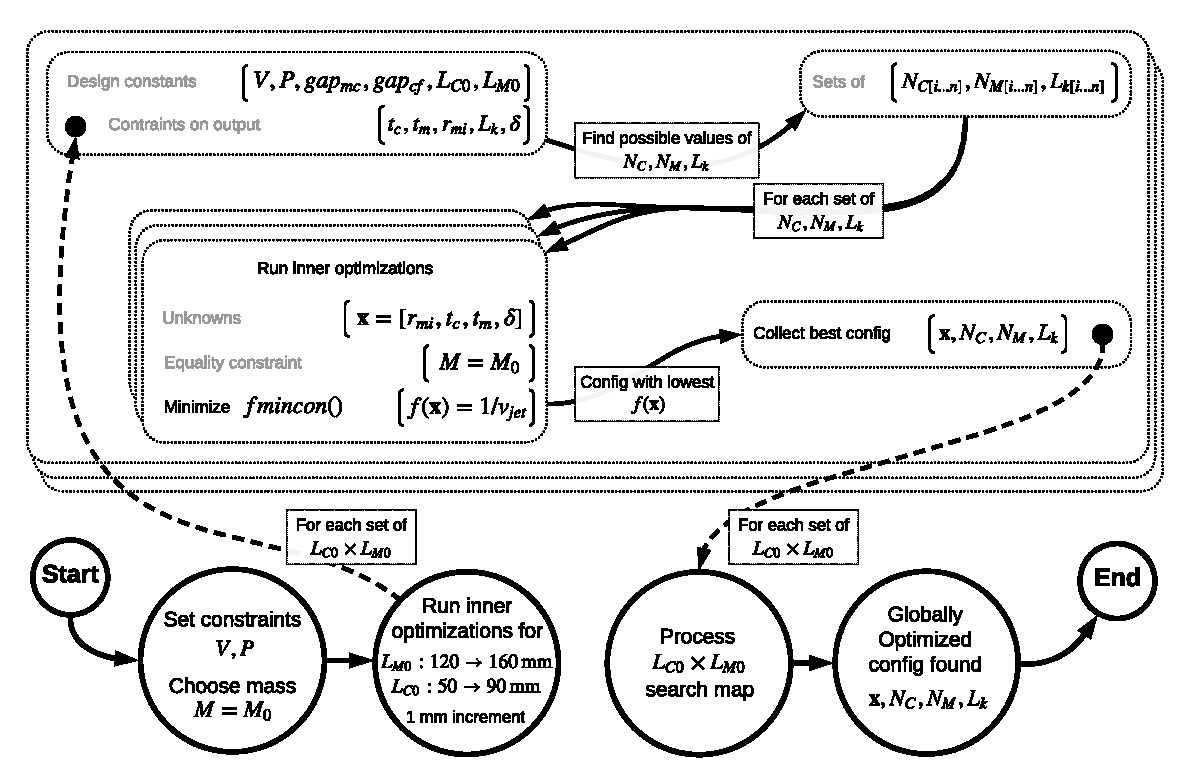
\includegraphics[width=5.8in]{chap3/images/HM_PMLSM_optimization.pdf}
              \caption{Summary of the top-level motor optimization algorithm and inner optimization routine. The algorithm uses motor specifications $V$, $P$, $M$ to determine the motor parameters $\textbf{x}=[r_{mi},t_c,t_m,\delta]$, $N_C$, $N_M$, $L_k$ at which the jet speed $v_{jet}$ can be maximized.}
              \label{fig:chapter/hm/top level optmization}
            \end{figure*}
            
            
            In summary, the outer optimization loop provides unique combinations of $L_{C0}$, $L_{M0}$, and $M_0$ to produce a set of possible $N_C$, as well as corresponding values of $N_M$ and $L_k$. At each point in the $L_{C0} \times L_{M0}$ space, multiple inner most optimizations will perform a non-linear constraint optimization for the unknown variable vector $\textbf{x}$:
            
            
            \begin{equation}
                \textbf{x} = \left[ r_{mi}, t_m, t_c, \delta\right]
                \label{eq:inner optimization x}
            \end{equation}
            
            
            Each inner optimization's aim is to find $\textbf{x}$ given $\left[N_C,N_M,L_k,M_0\right]$ from the outer optimization, and constants $\left[P,V\right]$ to maximize the jet speed $v_{jet}$ achieved where the same variable ranges in Table\,\ref{table:table_of_optimization_constraints_PMLSM} also apply: 
            
            
            \begin{equation}
                \begin{array}{rll}
                    \textbf{minimize}       & \small{objective\,\,function}     & f(\textbf{x})=\frac{1}{v_{jet}} \\
                    \textbf{subjected to}   & \small{equality\,\,constraint}    & h_1(\textbf{x})=M - M_0= 0
                \end{array}
                \label{eq:inner optimization for PMLSMs}
            \end{equation}
            
            
            
            With an unique set of $\left[\textbf{x}, N_C,N_M,L_k,M_0\right]$, the motor constant $K_m$ and motor mass $M$ can be found with the method outlined in Section\,\ref{Chapter:PMLSM design HM/electromagnetic model/hm solution}. Together with known power dissipation $P$, ampoule volume $V$, and water density $\rho_w$, the jet velocity $v_{jet}$ can be derived directly from Equation\,\ref{eq:power dissipation for PMLSMs}:
            
            
            \begin{equation}
                v_{jet} = \sqrt[4]{\frac{4P {K_m}^2 {L_S}^2}{\rho_w V^2}}
                \label{eq:v_jet}
            \end{equation}
            
            
            The inner optimization uses constrained nonlinear multi-variable optimization based on the interior point algorithm (MATLAB Optimization Toolbox) to minize the objective function in Equation\,\ref{eq:inner optimization for PMLSMs}. Upon finishing the inner optimizations for each pair $L_{C0} \times L_{M0}$, the control flow saves the best performing motor configuration and moves on to the next $L_{C0} \times L_{M0}$, obtains the next set of possible $N_C$ and so on. Fig.\,\ref{fig:chapter/hm/top level optmization} summarizes and illustrates both the outer and the inner optimization algorithms.
    
    
    % -----------------------------------------------------------------------------------
    % --- NEW SUB SECTION --- NEW SUB SECTION --- NEW SUB SECTION --- NEW SUB SECTION --- 
    % -----------------------------------------------------------------------------------
    \subsection{Results}                        \label{Chapter:PMLSM design HM/design optimization/results}
    
            
        The global optimization of \acs{PMLSM} for the problem described in Equation\,\ref{eq:outer optimization for PMLSMs} at different mass constraints $M_0=[325,350,375,400,425]\,\mathrm{g}$ is summarized in Table\,\ref{table:result for global optimization of PMLSM via HM method}.
            
            
        Taking an example for the global optimization of constraints set $P=1500\,\mathrm{W}$, $V=1\,\mathrm{mL}$, $gap_{mc}=1.2\,\mathrm{mm}$, $gap_{cf}=0.1\,\mathrm{mm}$, $M_0=325\,\mathrm{g}$ on the search space of $L_{M0}:120\,\mathrm{mm}\rightarrow 160\,\mathrm{mm}$, and $L_{C0}:50\,\mathrm{mm}\rightarrow 90\,\mathrm{mm}$, we found an under-hung motor with $N_C=4$, $N_M=12$, $L_k=26.5\,\mathrm{mm}$, $r_{mi}=2\,\mathrm{mm}$, $t_m=6.15\,\mathrm{mm}$, $t_c=3\,\mathrm{mm}$, $\delta=0.30$. The motor is able to theoretically produce $246.64\,\mathrm{N}$ at the rated power, which corresponds to a motor constant $K_m=6.37\,\mathrm{N/\sqrt{W}}$ and peak jet speed $v_{jet}=228.92\,\mathrm{m/s}$. The motor constant achieved by an optimized \acsp{VCM} of similar weight constraint is $3.6\,\mathrm{N/\sqrt{W}}$\,\cite{ruddy2014}. Even with additional lengths constraint is in place, \acs{PMLSM} still outperforms \acs{VCM} in power efficiency. The achievable jet speed $v_{jet}$ is beyond what is required for a successful needle free injection.
            
            
            \begin{landscape}
                \begin{table}
                    \renewcommand{\arraystretch}{1.2}
                    \caption{Summary of motor design optimization values and performance using \acs {HM} method}
                    \label{table:result for global optimization of PMLSM via HM method}
                    \centering
                    \begin{tabular}{lllrrrrr}
                        \hline
                        \textbf{Params}     & \textbf{Description}                            & \textbf{Unit}           & $M_0=\mathbf{325\,g}$ & $\mathbf{350\,g}$ & $\mathbf{375\,g}$ & $\mathbf{400\,g}$ & $\mathbf{425\,g}$ \\
                        \hline
                        $P$        & Power dissipation in coil winding      & $\mathrm{kW}$  & $1.50$                & $1.50$            & $1.50$            & $1.50$            & $1.50$            \\
                        $V$        & Volume of ampoule                      & $\mathrm{mL}$  & $1.00$                & $1.00$            & $1.00$            & $1.00$            & $1.00$            \\
                        $gap_{mc}$ & Magnet and coil fixed gap              & $\mathrm{mm}$  & $1.20$                & $1.20$            & $1.20$            & $1.20$            & $1.20$            \\
                        $gap_{cf}$ & Coil and iron fixed gap                & $\mathrm{mm}$  & $0.10$                & $0.10$            & $0.10$            & $0.10$            & $0.10$            \\
                        \hline
                        $L_{C0:optim}$ & Constraint $L_C$ winding at global optimum & $\mathrm{mm}$        & $53.00$                       & $53.00$           & $53.00$           & $53.00$           & $53.00$           \\
                        $L_{M0:optim}$ & Constraint $L_C+L_S$ at global optimum        & $\mathrm{mm}$        & $160.00$                      & $160.00$          & $160.00$          & $160.00$          & $160.00$          \\
                        \hline
                        $r_{mi}$   & Magnet array inner radius              & $\mathrm{mm}$  & $2.00$                & $2.00$            & $2.00$            & $2.00$            & $2.00$            \\
                        $t_m$      & Magnet thickness                       & $\mathrm{mm}$  & $6.15$                & $6.35$            & $6.67$            & $6.99$            & $7.29$            \\
                        $t_c$      & Coil thickness                         & $\mathrm{mm}$  & $3.00$                & $3.00$            & $3.00$            & $3.00$            & $3.00$            \\
                        $\delta$   & Ratio of radial magnet vs. magnet pair &                & $0.30$                & $0.25$            & $0.26$            & $0.26$            & $0.27$            \\
                        $N_C$      & Number of half coil-poles              &                & $4$                   & $3$               & $3$               & $3$               & $3$               \\
                        $N_M$      & Number of half magnet-poles            &                & $12$                  & $9$               & $9$               & $9$               & $9$               \\
                        \hline
                        $t_f$      & Iron shell thickness                   & $\mathrm{mm}$  & $0.77$                        & $1.07$            & $1.12$            & $1.15$            & $1.19$    \\       
                        $L_k$      & Full pole length                       & $\mathrm{mm}$  & $26.50$               & $35.33$           & $35.33$           & $35.33$           & $35.33$           \\
                        $L_C$      & Length of coil array                   & $\mathrm{mm}$  & $53.00$               & $53.00$           & $53.00$           & $53.00$           & $53.00$           \\
                        $L_M$      & Length of magnet array                 & $\mathrm{mm}$  & $159.00$              & $159.00$          & $159.00$          & $159.00$          & $159.00$          \\
                        $L_S$      & Stroke length                          & $\mathrm{mm}$  & $106.00$              & $106.00$          & $106.00$          & $106.00$          & $106.00$          \\
                        \hline
                        $v_{jet}$  & Achievable jet speed                   & $\mathrm{m/s}$ & $228.92$              & $234.20$          & $239.84$          & $245.13$          & $250.11$         \\
                        $F$        & Force exerts on piston                 & $\mathrm{N}$         & $246.64$                      & $258.72$          & $271.35$          & $283.44$          & $295.07$          \\
                        $K_m$      & Motor constant                         & $\mathrm{N/\sqrt{W}}$ & $6.37$                        & $6.68$            & $7.01$            & $7.32$            & $7.62$           \\
                        \hline
                    \end{tabular}
                \end{table}
            \end{landscape}
            
            
        \begin{figure}[!ht]
            \centering
            \subfloat[$M_0=325\,\mathrm{g}$. Global optimum found at $L_{C0}=53\,\mathrm{mm}$, $L_{C0}=160\,\mathrm{mm}$, $N_C=4$, and $N_M=12$.
            ]{
                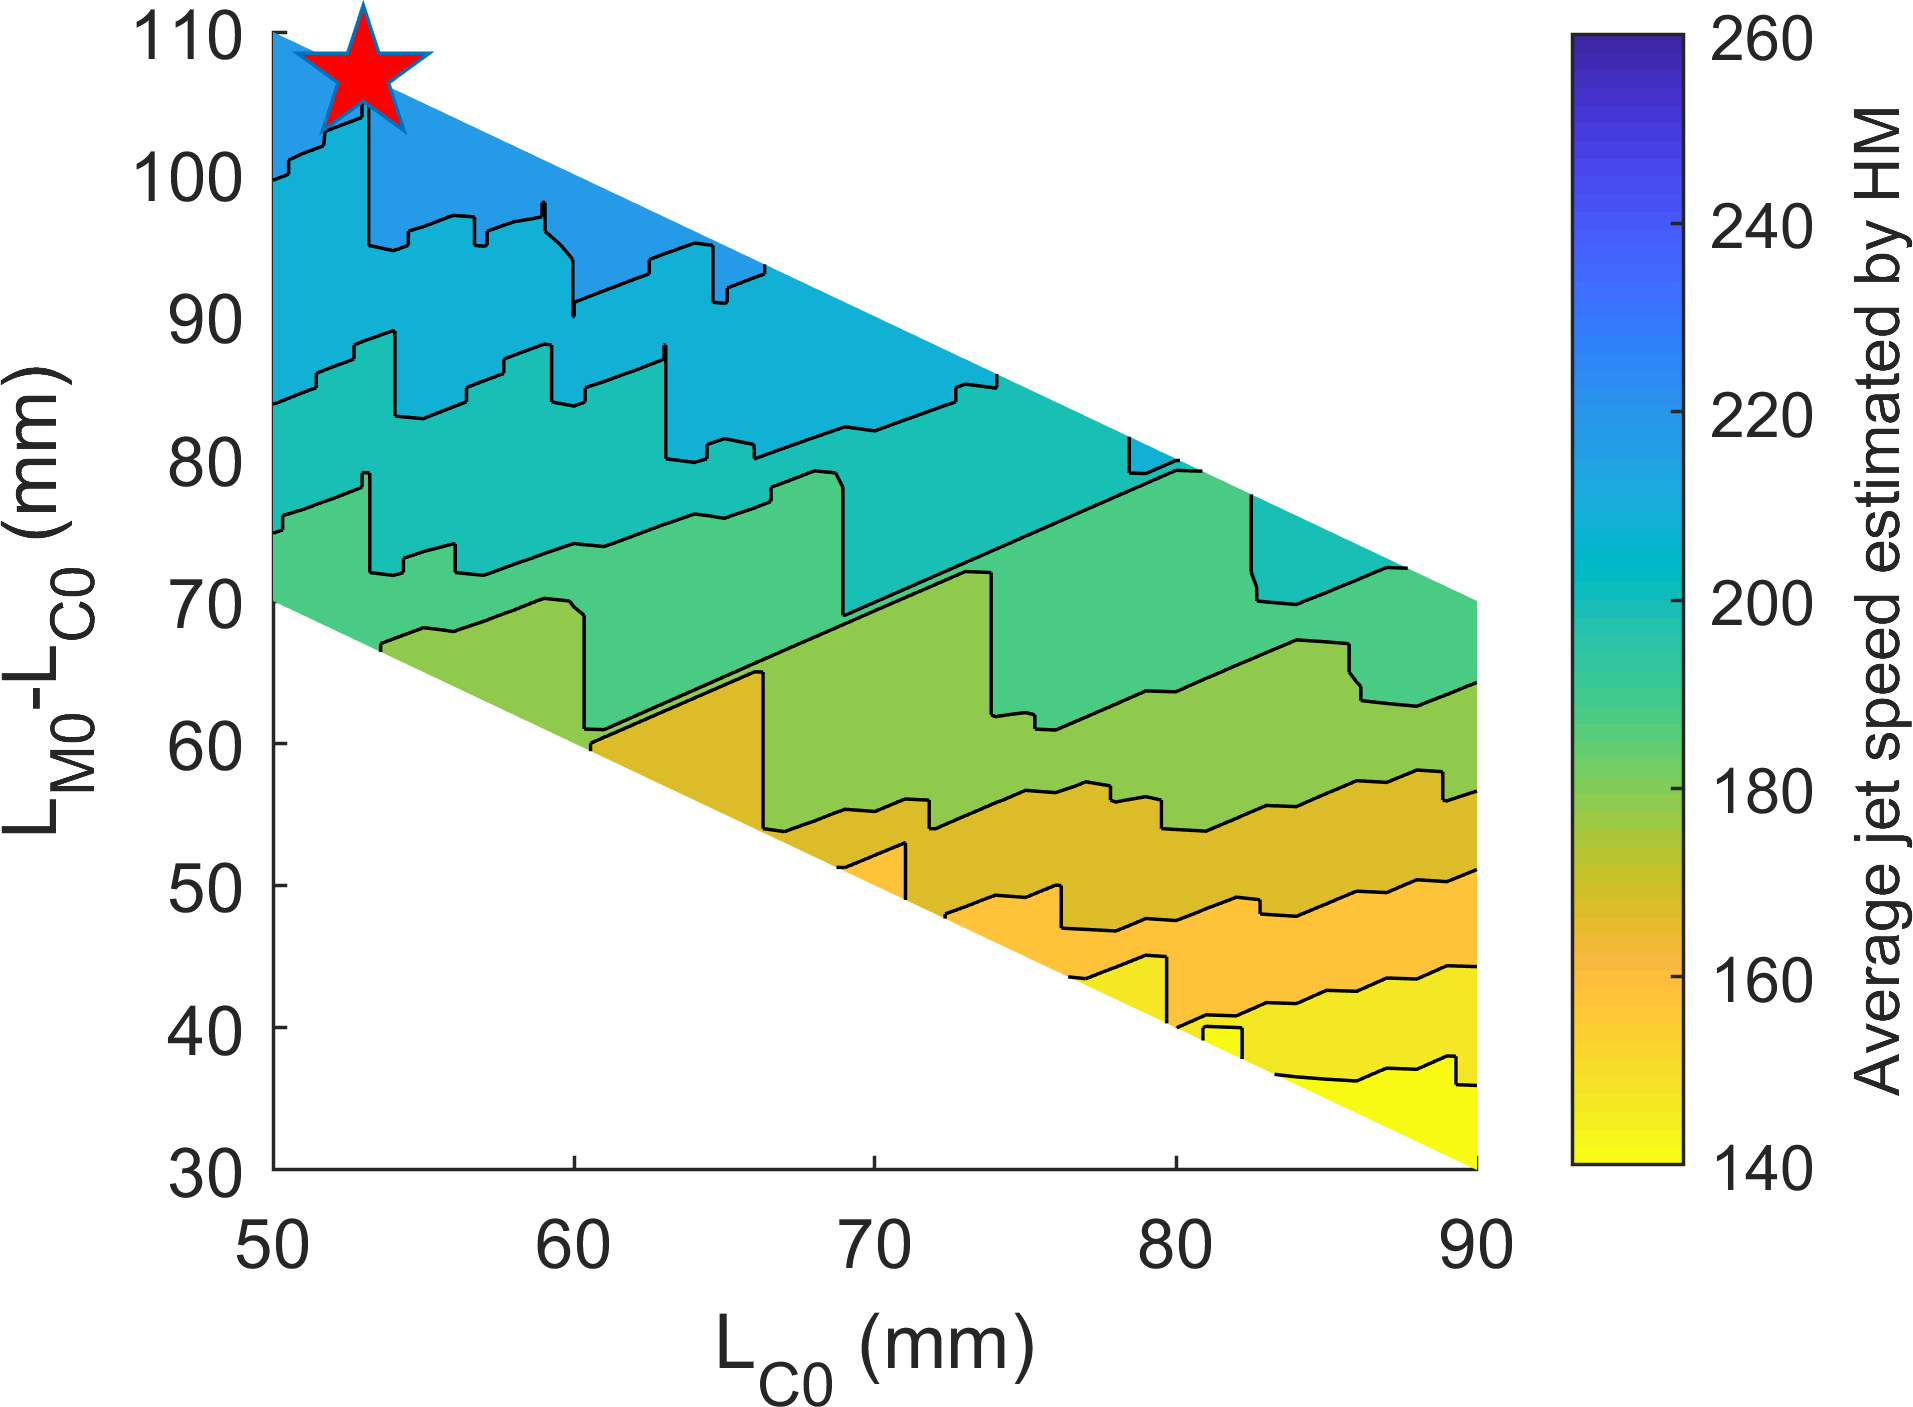
\includegraphics[width=0.45\textwidth]{chap3/images/PMLSM_HM_325g.png}
                \label{fig:chapter/hm/optimiization/325}
            }
            \qquad
            \subfloat[$M_0=350\,\mathrm{g}$ Global optimum found at $L_{C0}=53\,\mathrm{mm}$, $L_{C0}=160\,\mathrm{mm}$, $N_C=3$, and $N_M=9$.
            ]{
                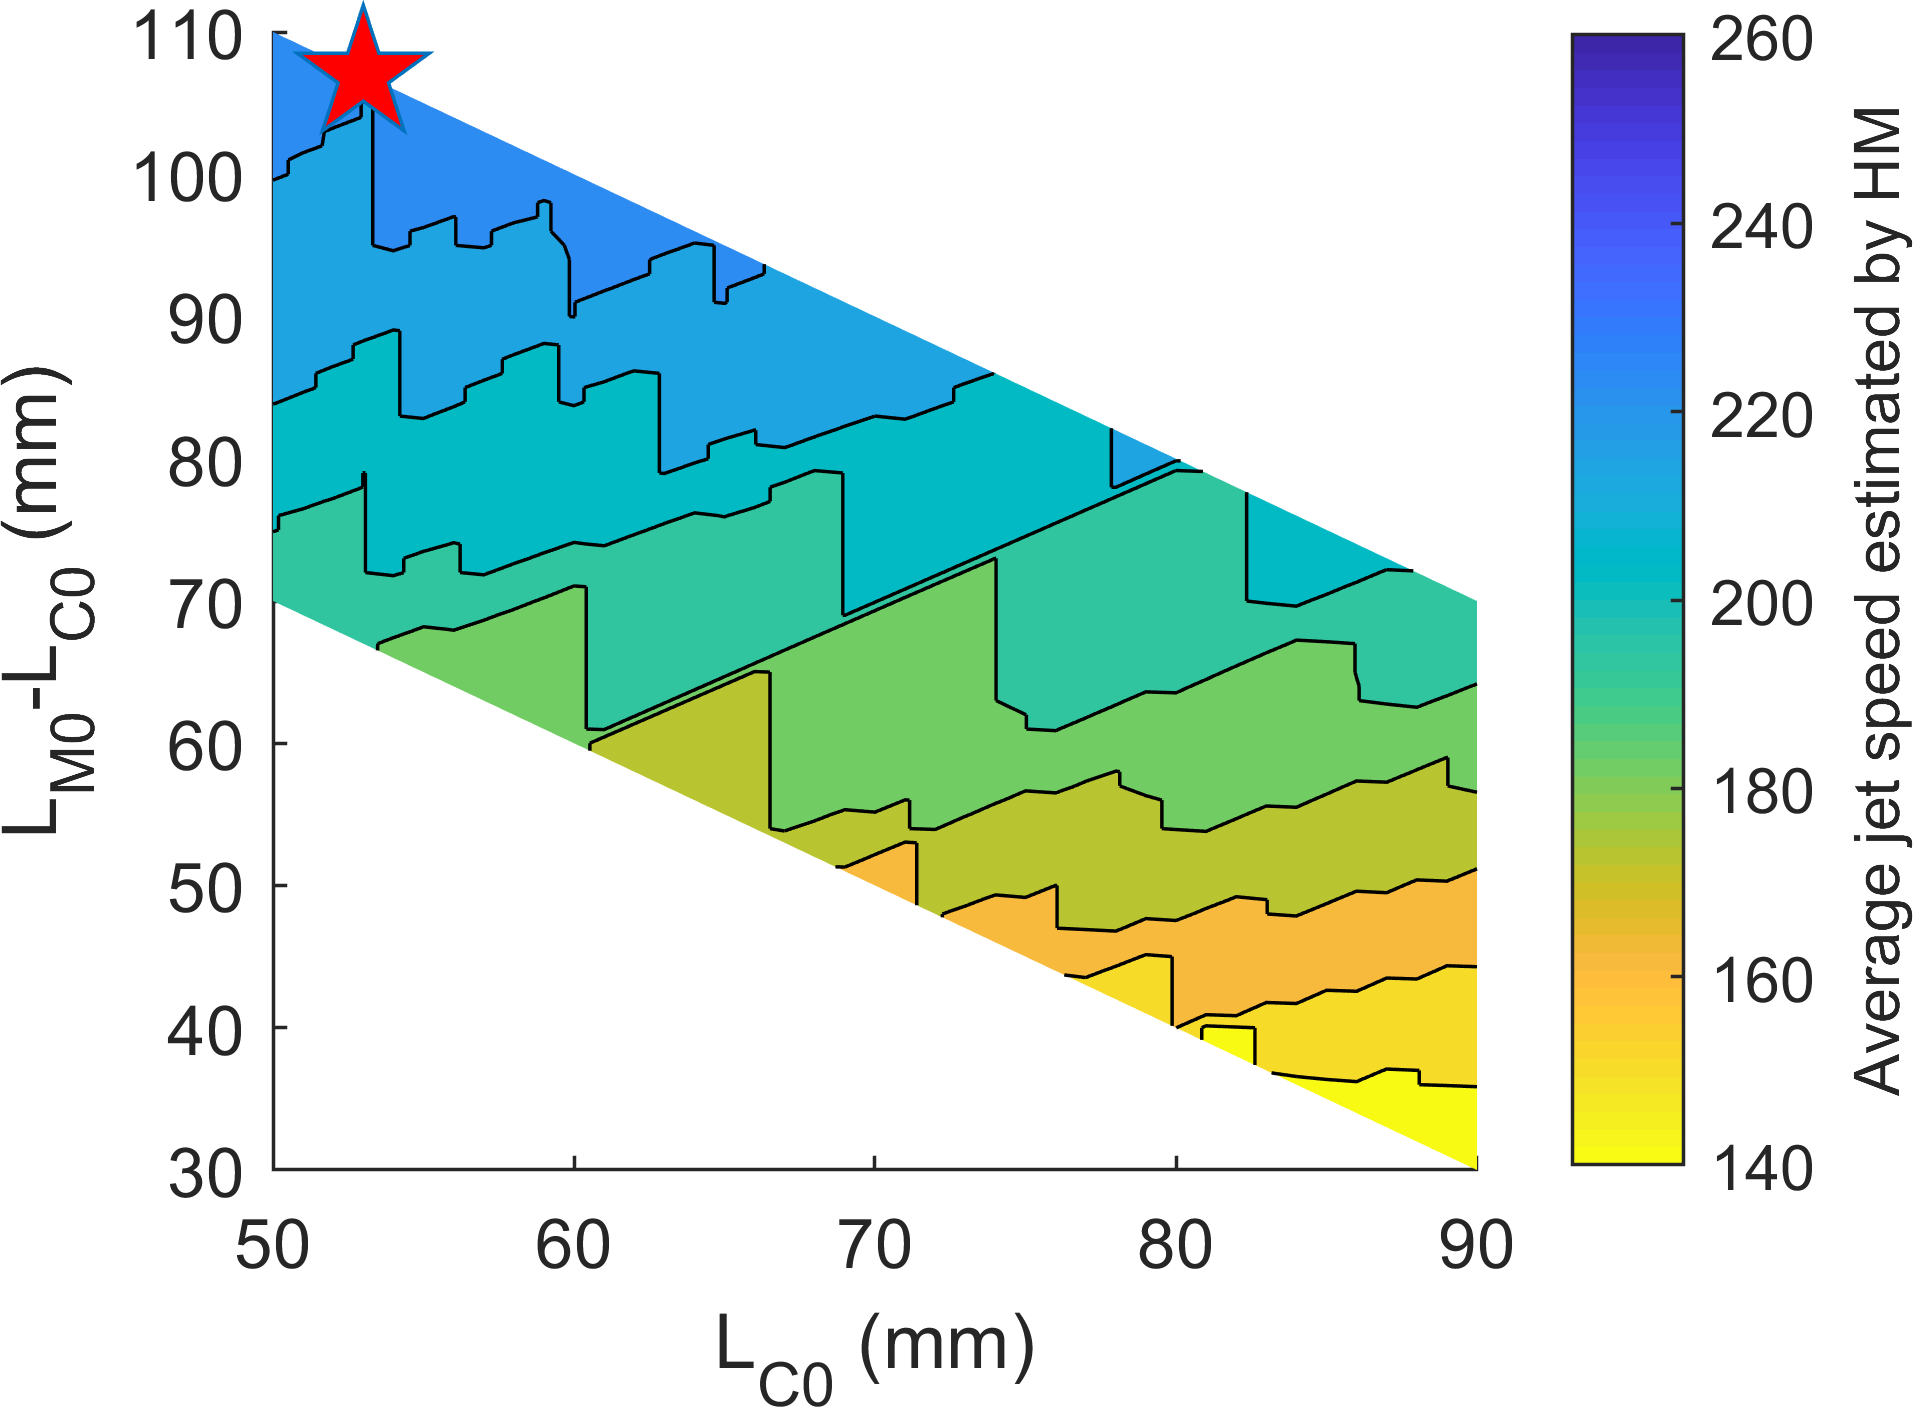
\includegraphics[width=0.45\textwidth]{chap3/images/PMLSM_HM_350g.png}
                \label{fig:chapter/hm/optimiization/350}
            }
            \\
            \subfloat[$M_0=375\,\mathrm{g}$. Global optimum found at $L_{C0}=53\,\mathrm{mm}$, $L_{C0}=160\,\mathrm{mm}$, $N_C=3$, and $N_M=9$.
            ]{
                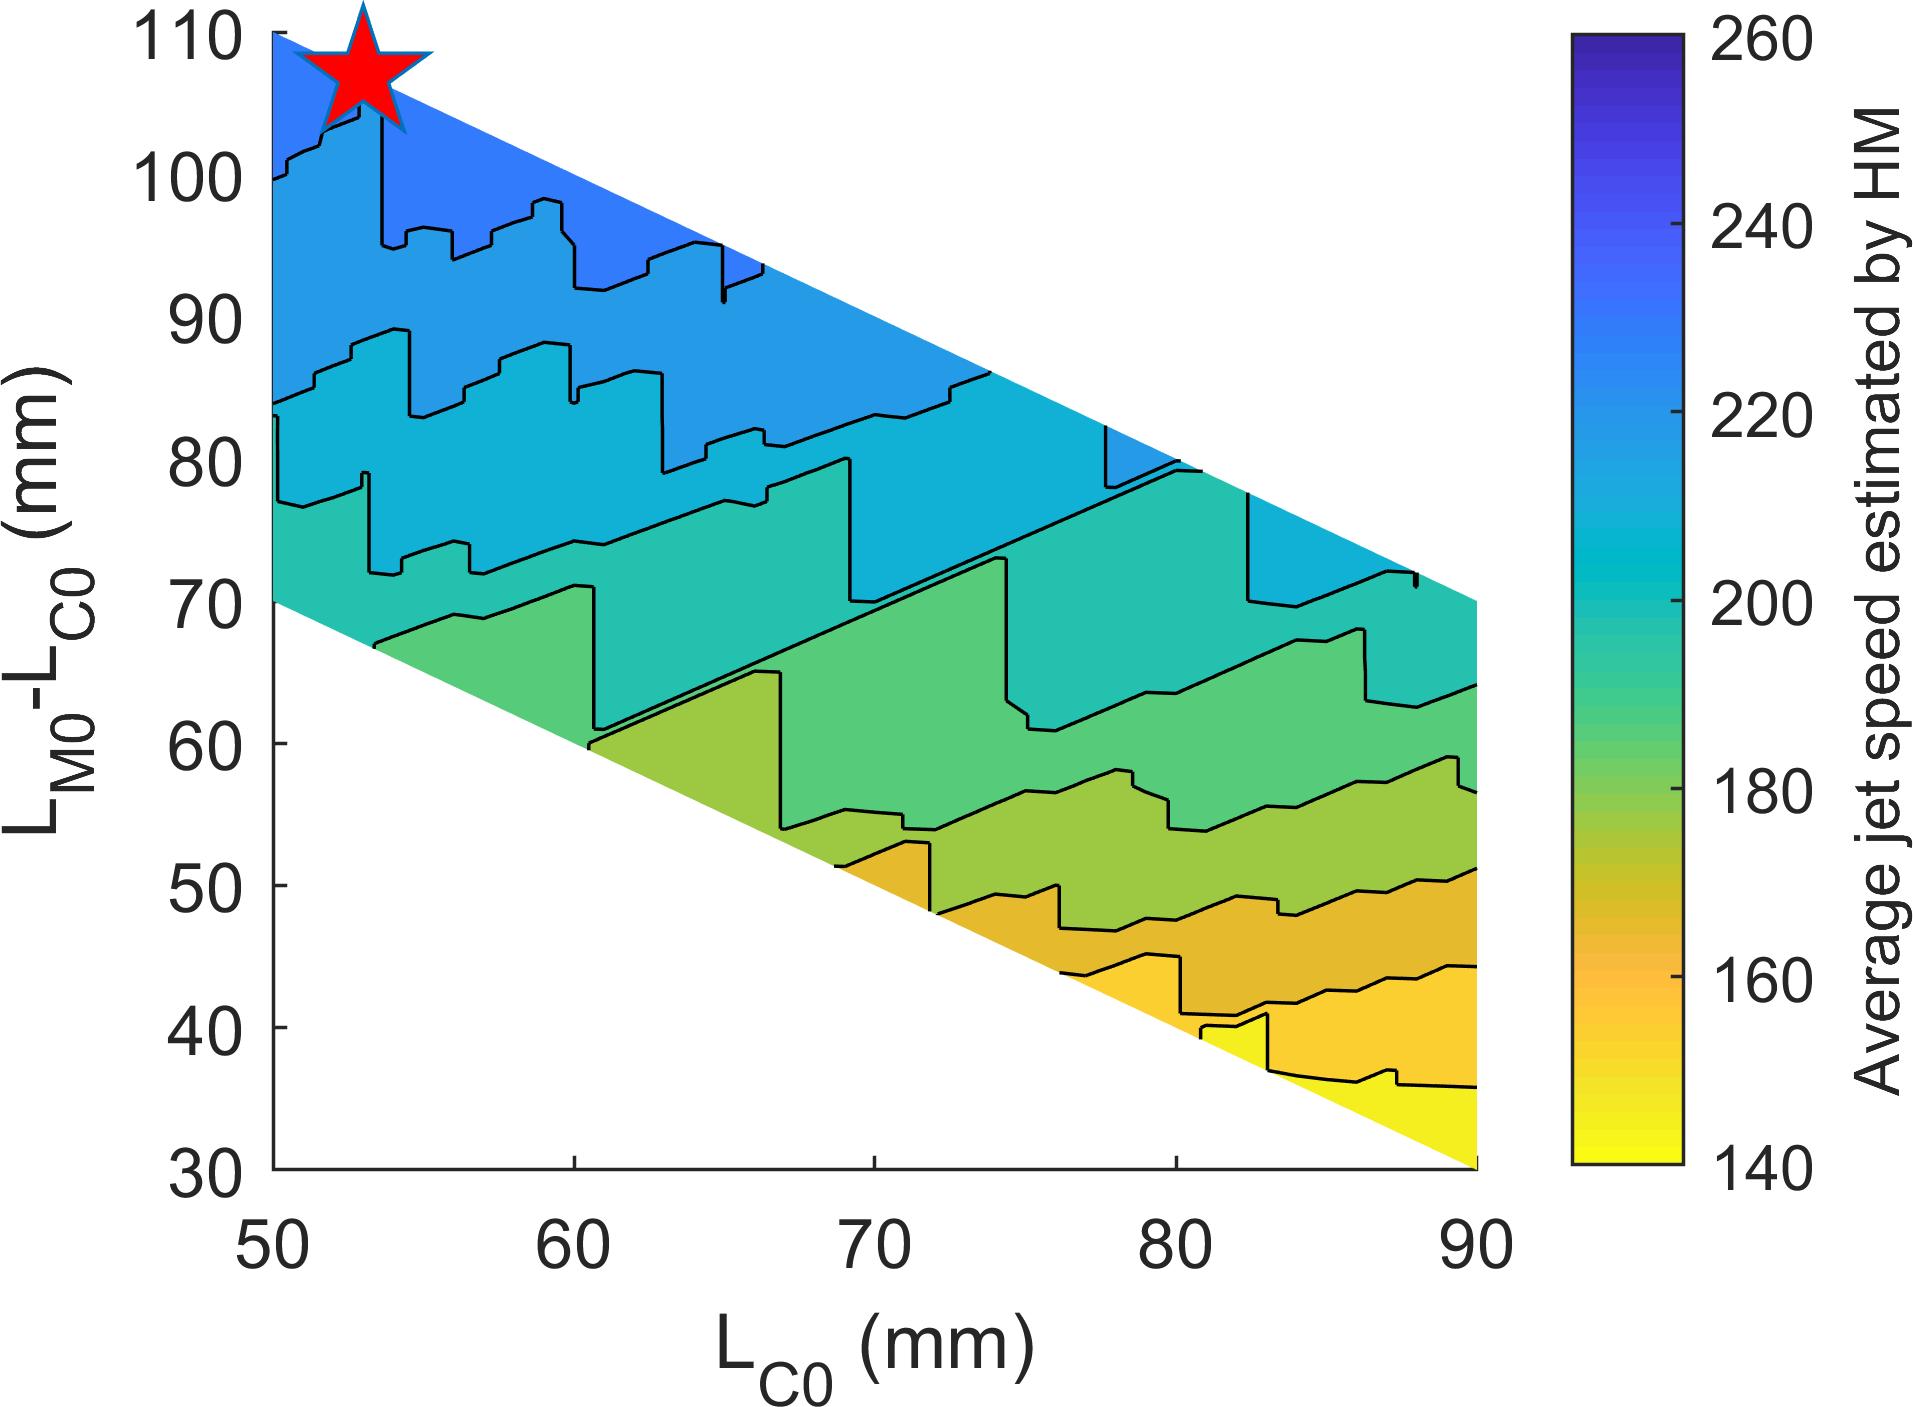
\includegraphics[width=0.45\textwidth]{chap3/images/PMLSM_HM_375g.png}
                \label{fig:chapter/hm/optimiization/375}
            }
            \qquad
            \subfloat[$M_0=400\,\mathrm{g}$. Global optimum found at $L_{C0}=53\,\mathrm{mm}$, $L_{C0}=160\,\mathrm{mm}$, $N_C=3$, and $N_M=9$.
            ]{
                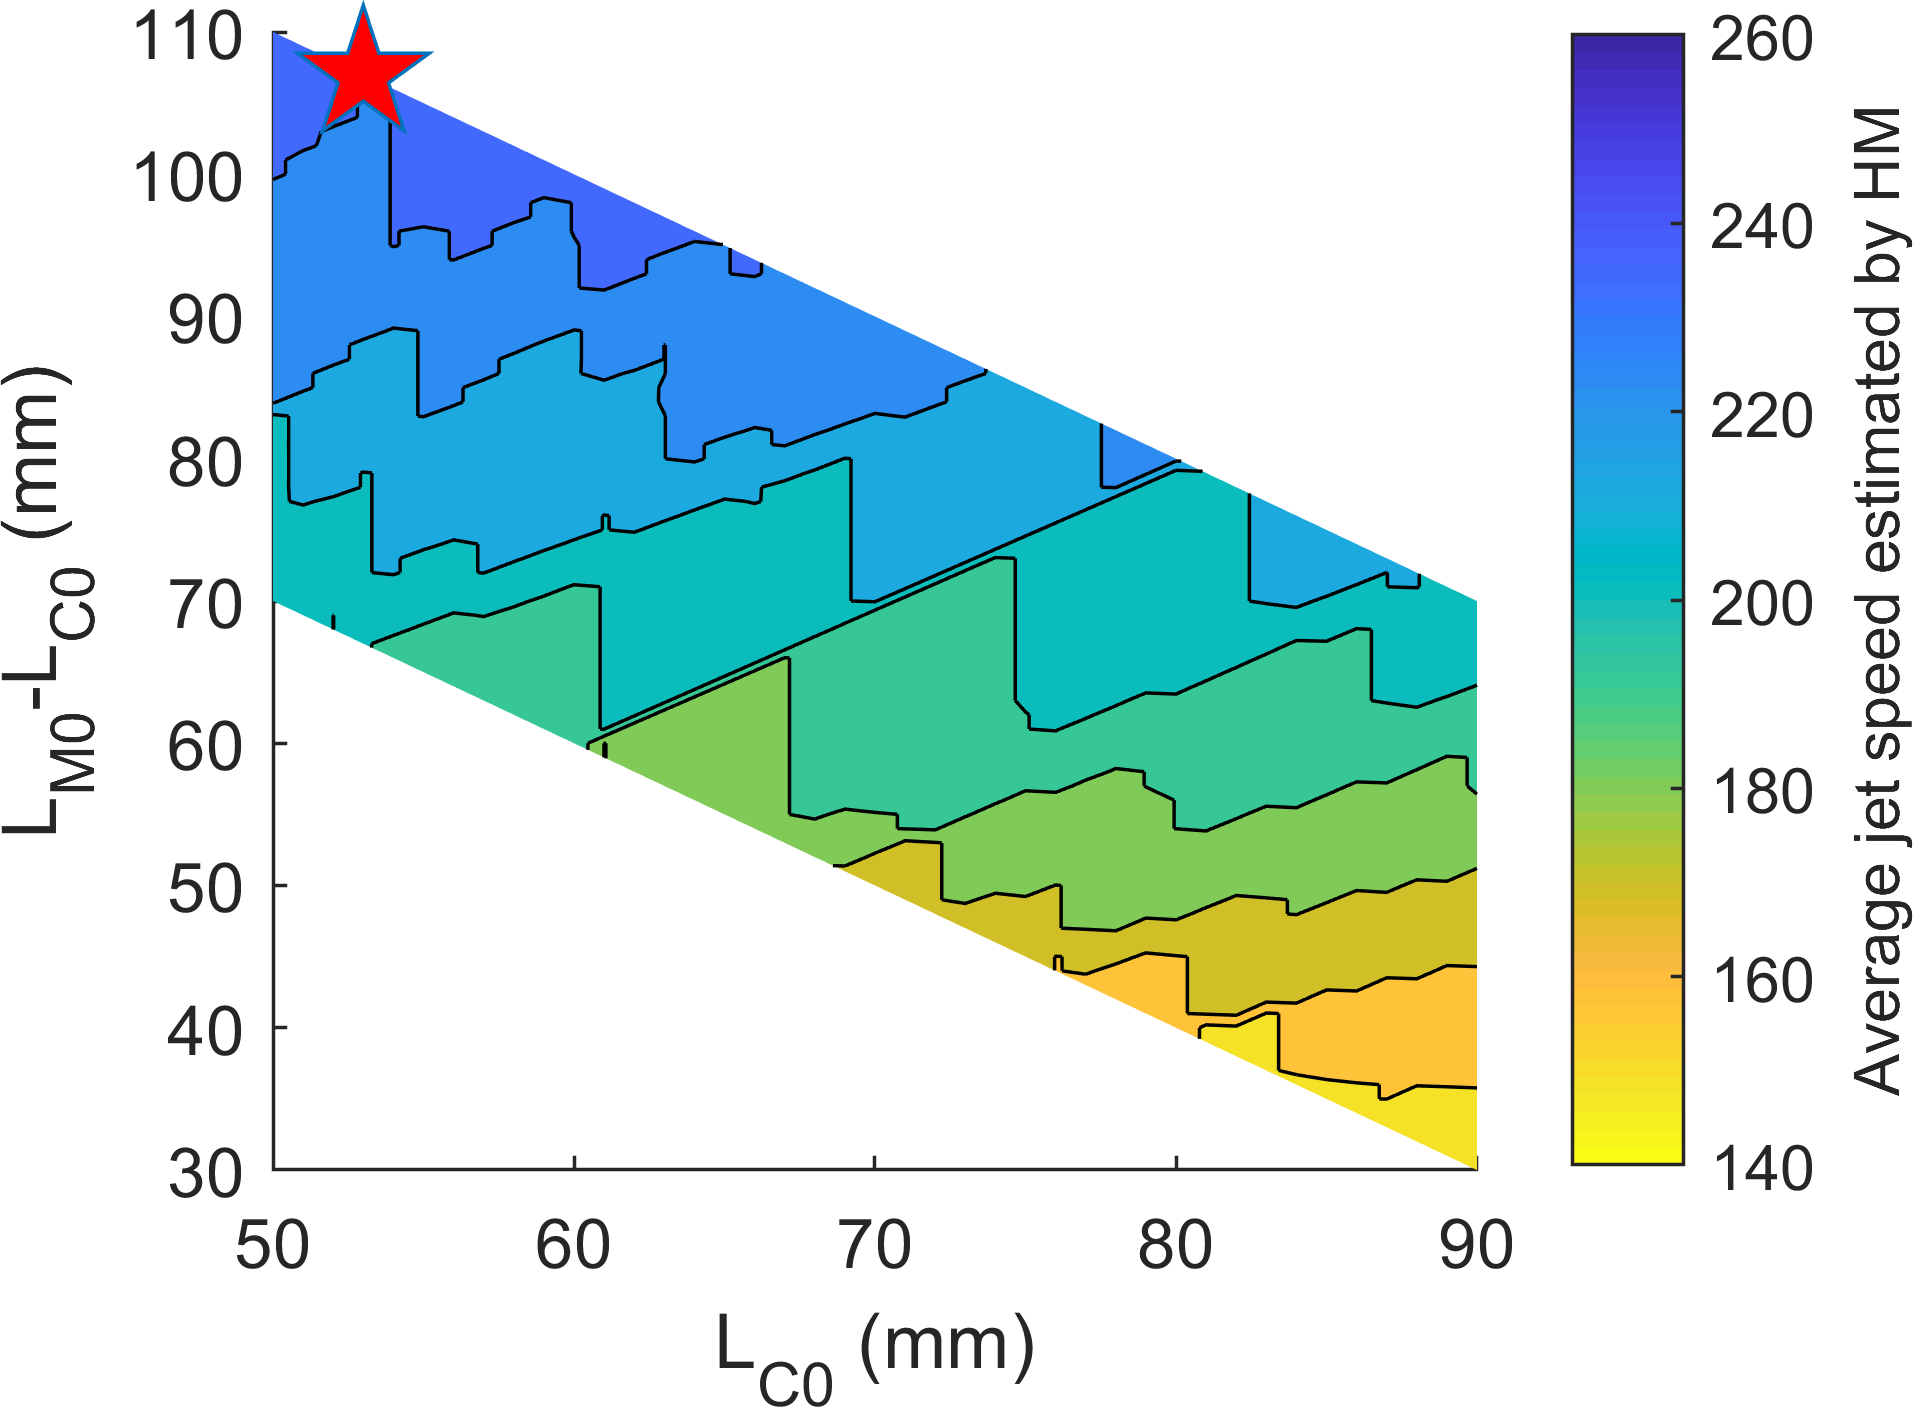
\includegraphics[width=0.45\textwidth]{chap3/images/PMLSM_HM_400g.png}
                \label{fig:chapter/hm/optimiization/400}
            }
            \\
            \subfloat[$M_0=425\,\mathrm{g}$. Global optimum found at $L_{C0}=53\,\mathrm{mm}$, $L_{C0}=160\,\mathrm{mm}$, $N_C=3$, and $N_M=9$.
            ]{
                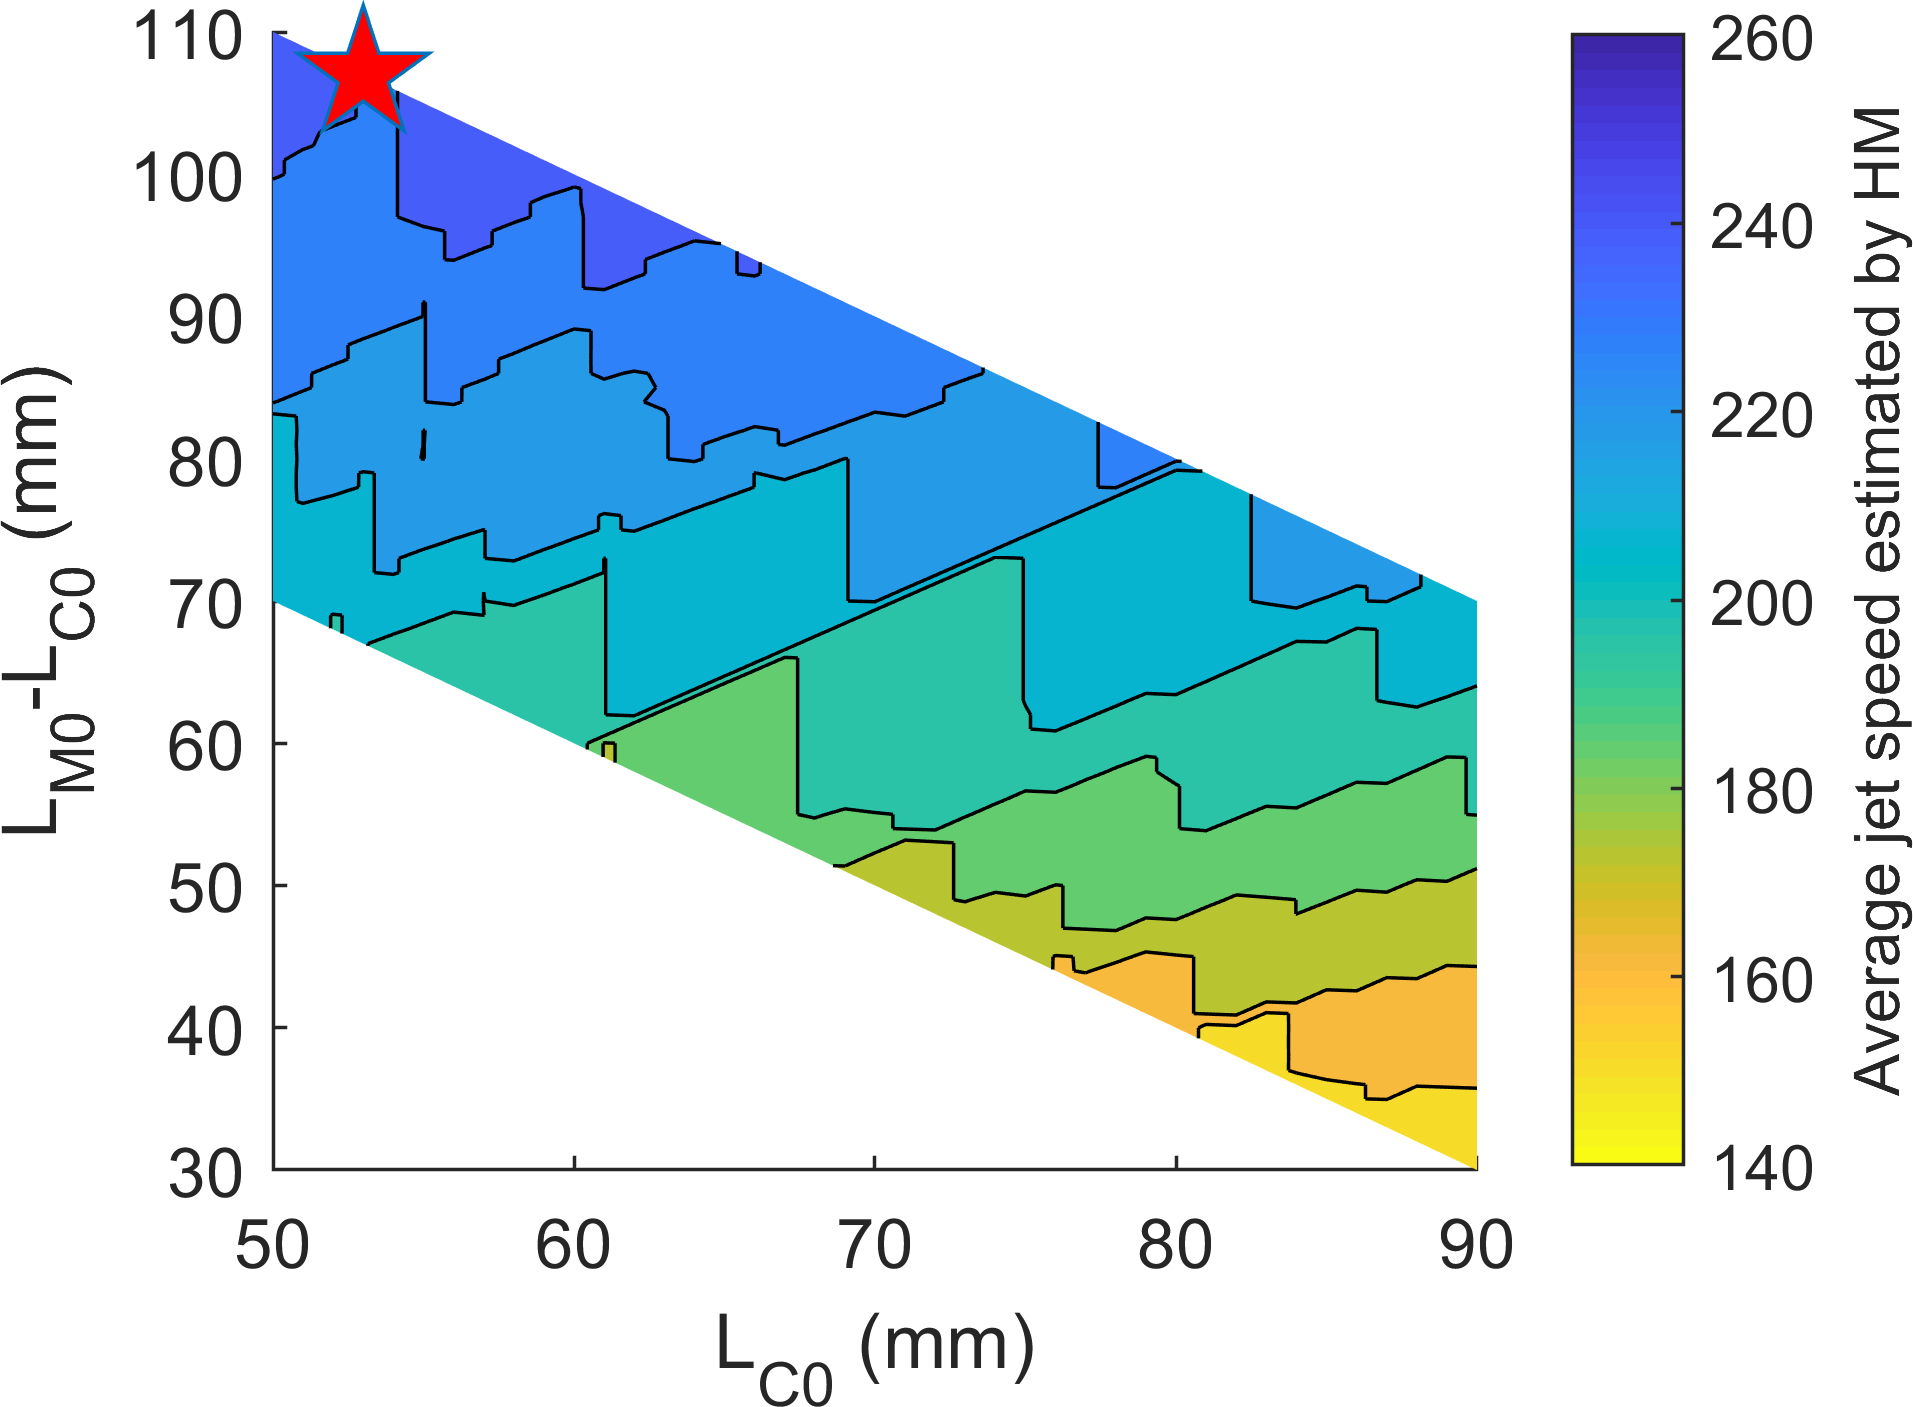
\includegraphics[width=0.45\textwidth]{chap3/images/PMLSM_HM_425g.png}
                \label{fig:chapter/hm/optimiization/425}
            }
            \\
            \caption{
                The global optimization plots of $v_{jet}$ for the search space $L_{M0}:120\,\mathrm{mm}\rightarrow 160\,\mathrm{mm} \times L_{C0}:50\,\mathrm{mm}\rightarrow 90\,\mathrm{mm}$ using $P=1500\,\mathrm{W}$, $V=1\,\mathrm{mL}$, $gap_{mc}=1.2\,\mathrm{mm}$, $gap_{cf}=0.1\,\mathrm{mm}$,  and $M_0$ of: (a) $325\,\mathrm{g}$, (b) $350\,\mathrm{g}$, (c) $375\,\mathrm{g}$, (d) $400\,\mathrm{g}$, and (e) $425\,\mathrm{g}$.
            }   \label{fig:chapter/hm/optimization search space result for differnt mass}
        \end{figure}
        
            
        According to Equation\,\ref{eq:power dissipation for PMLSMs}, and provided that $P$, $\rho_w$, $K_m$, $L_S$ are unchanged:
            
            
        \begin{equation}
            v_{jet}\propto\frac{1}{\sqrt{V}}
            \label{eq:v_jet and V}
        \end{equation}
            
            
        \begin{equation}
            V_{new}={\bigg(\frac{v_{jet:old}}{v_{jet:new}} \bigg)}^2 V_{old}
            \label{eq:v_jet and V ratio}
        \end{equation}
        
        

            
            
        If we now choose to adjust the ampoule cross-sectional area to reduce the peak jet speed $v_{jet}$ to $200\,\mathrm{m/s}$, the maximum volume $V$ of drug delivery can now be $V_{new}=1.31\,\mathrm{mL}$. 
            
            
        As expected, the more relaxed the mass constraint $M_0$, the higher the achievable jet speed $v_{jet}$ can be. Globally optimized motors at mass constraints $M_0$ of $350\,\mathrm{g}$, $350\,\mathrm{g}$, $375\,\mathrm{g}$, $400\,\mathrm{g}$, and $425\,\mathrm{g}$ can produce $v_{jet}$ of $229\,\mathrm{m/s}$, $234\,\mathrm{m/s}$, $240\,\mathrm{m/s}$, $245\,\mathrm{m/s}$, and $250\,\mathrm{m/s}$, respectively. Fig.\,\ref{fig:chapter/hm/optimization search space result for differnt mass} provides global optimization plots of $v_{jet}$ for the search space $L_{M0}:120\,\mathrm{mm}\rightarrow 160\,\mathrm{mm} \times L_{C0}:50\,\mathrm{mm}\rightarrow 90\,\mathrm{mm}$ using $P=1500\,\mathrm{W}$, $V=1\,\mathrm{mL}$, $gap_{mc}=1.2\,\mathrm{mm}$, $gap_{cf}=0.1\,\mathrm{mm}$,  and $M_0=[325,350,375,400,425]\,\mathrm{g}$. 
        
        Although the 2D contour patterns appear similar across the different plots, the color shade gradually gets darker with easier mass constraints $M_0$, indicating an increase in the motor performance as the response to easing the mass constraint. The ring patterns of the optimization search space contour plot appears non-convex with many steps and sudden changes. This is due the rounding operation such as $ceil$ and $floor$ on the number of armature and secondary repeats $N_C$, and $N_M$. It is also worth noticing that the optimums are found closed to the edge the $L_{M0} \times L_{C0}$ search space. This means that the performance of the optimum motor configurations found are limited by the constraints placed. In the case that the optimization constraints could be relaxed, a marginal performance gain would be realized. 


    % ===================================================================================================
    % === NEW SECTION === NEW SECTION === NEW SECTION === NEW SECTION === NEW SECTION === NEW SECTION ===
    % ===================================================================================================
    \section{Discussion}                            \label{Chapter:PMLSM design HM/discussion}
    
        
        To summarize, this chapter provides a semi-analytical solution for the electromagnetic model of slotless tubular \acsp{PMLSM} (Section\,\ref{Chapter:PMLSM design HM/electromagnetic model}), an efficient optimization scheme for a fixed motor mass at a given power dissipation (Section\,\ref{Chapter:PMLSM design HM/design optimization/optimization formulation}). Utilizing these modeling and optimization methodologies, we performed a case study and found globally optimized motor configurations for \acs{NFJI} under different mass constraints (Section\,\ref{Chapter:PMLSM design HM/design optimization/optimization formulation}). The optimized motor configuration for these requirements is summarized in Table~\ref{table:result for global optimization of PMLSM via HM method}. Most importantly, this work was able to confirm that \acsp{PMLSM} readily outperform \acsp{VCM} in \acs{NFJI} applications, being able to deliver more volume with far less energy. 
        
        
        The optimization benchmark optimization specification established in Section\,\ref{Chapter:PMLSM design HM/design optimization/design citeria} is especially important, and will be reused in accessing and comparing other types of \acsp{LSDDM} in the later Chapter\,\ref{Chapter:PMLSM design RSM}. With this modelling approach, it is assumed that the end-effect is ignored. Therefore the true performance will be slightly lower than the performance predicted by this modelling method\,\cite{Ruddy2013a}.
        
        
    \chapter{\acsp{LSDDM} design with Response Surface Modelling}   \label{Chapter:PMLSM design RSM}


    The concept of a “metamodel” is introduced as a reasonably accurate surrogate model, constructed via \acf{RSM} and powered by reduced-order models, deep neural networks, or statistically derived models. This chapter aims toward providing and applying an end-to-end \acs{RSM} design process that is viable for selected motor topologies: \acf{PMLSM}, \acf{LFSM}, and \acf{LTFM}. This process should be both specific and flexible enough to make a fair comparison between these types of motors in \acs{NFJI} applications. In order to achieve this goal, Section\,\ref{Chapter:RSM/outline} thoroughly investigates the \acs{RSM} method to establish a suitable design process. Then, Sections\,\ref{Chapter:RSM/PMLSM}, \ref{Chapter:RSM/LFSM}, and \ref{Chapter:RSM/LTFM} look at applying the established process for the selected types of motors. The optimization problem statement, the objective function and the high-level constraints for each motor topology explored in this chapter are equivalent to the optimization problem already established in Section\,\ref{Chapter:PMLSM design HM/design optimization/optimization formulation/out} and Equation\,\ref{eq:outer optimization for PMLSMs}. By comparing optimization results for \acsp{PMLSM} obtained in Section\,\ref{Chapter:PMLSM design HM/design optimization/results} and Section\,\ref{Chapter:RSM/PMLSM}, a fair indicator for the accuracy and correctness of the \ac{RSM} method is gathered. Toward the end of this chapter, Section\,\ref{Chapter:RSM/discussion} aggregates the results collected in the previous optimization runs of different types of motors in order to choose the most suitable type of linear synchronous motor for \acs{NFJI} application.


    % ===================================================================================================
    % === NEW SECTION === NEW SECTION === NEW SECTION === NEW SECTION === NEW SECTION === NEW SECTION ===
    % ===================================================================================================
    \section{Process outline}                        \label{Chapter:RSM/outline}
    
    
        \acf{DOE} together with \ac{RSM} have been applied to many engineering problems. These studies often include statistical processes to investigate how the input correlates to the output, and which inputs have the greatest effect on the outputs. In applications where the cost of acquiring an actual input and output pair is expensive, \ac{DOE} sampling methods are helpful in reducing the data acquisition cost. 
        
        
        \ac{DOE} sampling methods can be divided into two classes: Factorial designs and Taguchi methods. Factorial designs include a full factorial, where all possible combinations of the factor levels are investigated, or only part of the full factorial are selected for acquisition. A full factorial is very useful because it allows the data analyst to observe the effects of changing the factor by providing all the available data interactions. It is recommended to use full factorial when possible. On the other hand, fractional factorial designs reduce the accuracy of the analysis in exchange for a lower data acquisition cost. In reality, an experiment can have full factorials for some inputs and fractional factorials for less important inputs. Taguchi methods use orthogonal arrays to gain detailed information about effects of factors with the minimum number of experiments. As a result, Taguchi methods, with fewer simulations, provide an important cost advantage to factorial designs. 
        
        
        In a high order \ac{RSM} problems with many input variables, reaching a large sampling levels set for each input is the key to producing accurate model predictions. However, the time and computation effort required to reach the high sampling levels grow exponentially with the number of input parameters. Only when the data acquisition budget allows, obtaining an extra set of data based on a set of randomly generated input sets will be helpful in increasing the "metamodel" accuracy. In this body of work, the method of constructing and inferring deep regression \acf{ANN} is employed to train the most accurate and generalized models that could be achieved.
        
        
        All types of motor topology studies in this chapter follow the common design criteria established in Section\,\ref{Chapter:PMLSM design HM/design optimization/design citeria}. The overall \ac{RSM} process to be applied widely in this chapter is outlined as follow:
        
        
        \begin{itemize}
            \item RSM problem statement - starting from topology, this step defines and selects the design parameters, value ranges and sampling level of the parameters,
            \item Data mining - constructs the experiment with the sampling levels previously obtained, then acquire the training data via a selected computational method (be it Harmonic Modelling or Finite Element Analysis) for a single repeating unit,
            \item Model fitting - trains/fits the training data into an \ac{ANN} that best represents the motor topology at hand in the range of values already specified,
            \item Optimization - performs convex non-linear optimization that utilizes the \ac{ANN} model trained earlier.
        \end{itemize}
        

    % ===================================================================================================
    % === NEW SECTION === NEW SECTION === NEW SECTION === NEW SECTION === NEW SECTION === NEW SECTION ===
    % ===================================================================================================
    \section{Application to \ac{PMLSM}}             \label{Chapter:RSM/PMLSM}
    
        
        In this section, the aim of the work is to examine the effectiveness of the proposed design process by comparing optimization results obtained by the \acs{HM} method, to the optimization results obtained by the \acs{RSM} method. Fig.\,\ref{fig:chapter/rsm/PMLSM optimization} illustrates the \acs{RSM} design process adapted to the \acs{PMLSM} topology already presented in \ref{Chapter:PMLSM design HM/electromagnetic model/topology}. 
        
        
        \begin{figure*}[h]
            \centering
            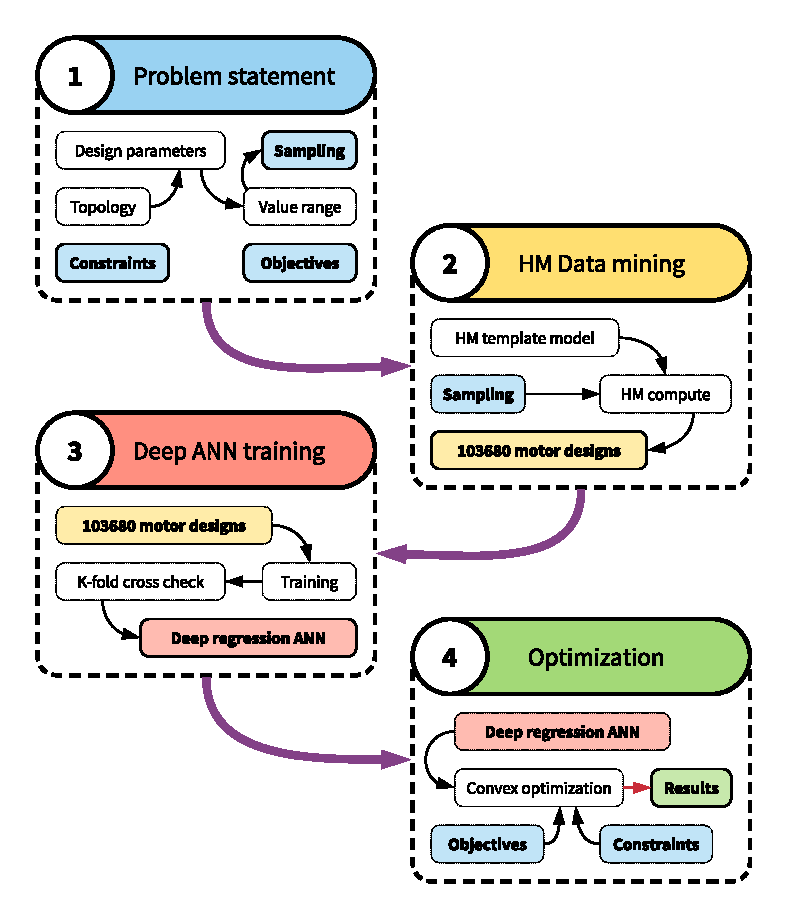
\includegraphics[width=4.5in]{chap4/images/optimization_process_RSM_for_PMLSM.pdf}
            \caption{Flowchart of the RSM motor design process adapted for PMLSM.}
            \label{fig:chapter/rsm/PMLSM optimization}
        \end{figure*}
        
        
        % -----------------------------------------------------------------------------------
        % --- NEW SUB SECTION --- NEW SUB SECTION --- NEW SUB SECTION --- NEW SUB SECTION --- 
        % -----------------------------------------------------------------------------------
        \subsection{Specifications \& Samplings}    \label{Chapter:RSM/PMLSM/spec}
        
        
            Re-using the considerations of the \acs{PMLSM} topology already presented in Section\,\ref{Chapter:PMLSM design HM/electromagnetic model/topology}, this work refers back to the design parameters $t_c$, $t_m$, $r_{mi}$, $L_k$, $\delta$ and their accompanying value ranges listed in Table\,\ref{table:table_of_optimization_constraints_PMLSM}. Additionally, the magnet to coil gap $gap_{mc}$ and coil to iron gap $gap_{cf}$ are addressed as constant values. 
            
            
            Table.\,\ref{table:RSM design level for PMLSM} shows incremental sampling steps for the structural design factors. From the sampling steps, a full factorial design grid of $51840$ designs was generated. Additionally, the same number of design cases were constructed by random input variables in the ranges specified by Table\,\ref{table:RSM design level for PMLSM}. The purpose of combining the factorial design space and the randomly generated design cases is to help generalize the supposedly continuous \acs{RSM} response better. In total, there were $103680$ independent motor designs available for \acs{ANN} training. To maximize the re-usability of the data collected, the obvious choice is to use \acs{HM} to generate a library of design for motors with only a single repeating unit. All of these motor designs were assumed to have the number of half coil periods $N_C$ and the number of half magnet periods $N_M$ of $1$. The input power was also to be kept at $P=1500\mathrm{W}$, in order to directly compare with the study in Chapter\,\ref{Chapter:PMLSM design HM}.
            
            
            \begin{table}[!h]
                \renewcommand{\arraystretch}{1.2}
                \caption{Summary of motor parameter sampling levels for \acs{RSM} of \acs{PMLSM}}
                \label{table:RSM design level for PMLSM}
                \centering
                \begin{tabular}{@{}l r r r r r r r@{}}
                \hline
                \bfseries Params & \bfseries Level 1 & \bfseries Jump step & \bfseries Last level & \bfseries Unit \\
                \hline
                    $L_k$       &   18     &   2     &   90     &   $\mathrm{mm}$\\
                    $r_{mi}$    &    2     &   2     &   10     &   $\mathrm{mm}$\\
                    $t_m$       &    2     &   2     &   20     &   $\mathrm{mm}$\\
                    $t_c$       &    3     &   2     &   19     &   $\mathrm{mm}$\\
                    $\delta$    &  0.1     & 0.1     &  0.6     &   \\
                \hline
                \end{tabular}
            \end{table}
        
        
        % -----------------------------------------------------------------------------------
        % --- NEW SUB SECTION --- NEW SUB SECTION --- NEW SUB SECTION --- NEW SUB SECTION --- 
        % -----------------------------------------------------------------------------------
        \subsection{\acs{HM} data mining}           \label{Chapter:RSM/PMLSM/data mining}
        
        
            The base \acs{HM} computation model in Section\,\ref{Chapter:PMLSM design HM/electromagnetic model/hm solution} was re-purposed to help generate motor design data. To facilitate for the data mining and the optimization process later on, the same electromagnetic model was converted into a re-usable function as illustrated in Fig.\,\ref{fig:chapter/rsm/PMLSM/mining process}. The free inputs included the repeat length $L_k$, the inner radius of the cylindrical magnet array $r_{mi}$, the magnet radial thickness $t_m$, the coil radial thickness $t_c$, and the proportion of the radially magnetized magnet against the total length of the magnet. The fixed input included the number of half coil-phase $N_C$, the number of half magnet-phase $N_M$, and the power $P$. On the output side, the data mining function provided the half repeating unit mass $M$, motor constant $K_m$ and the linear force produced $F$.
        
        
            \begin{figure}
                \centering
                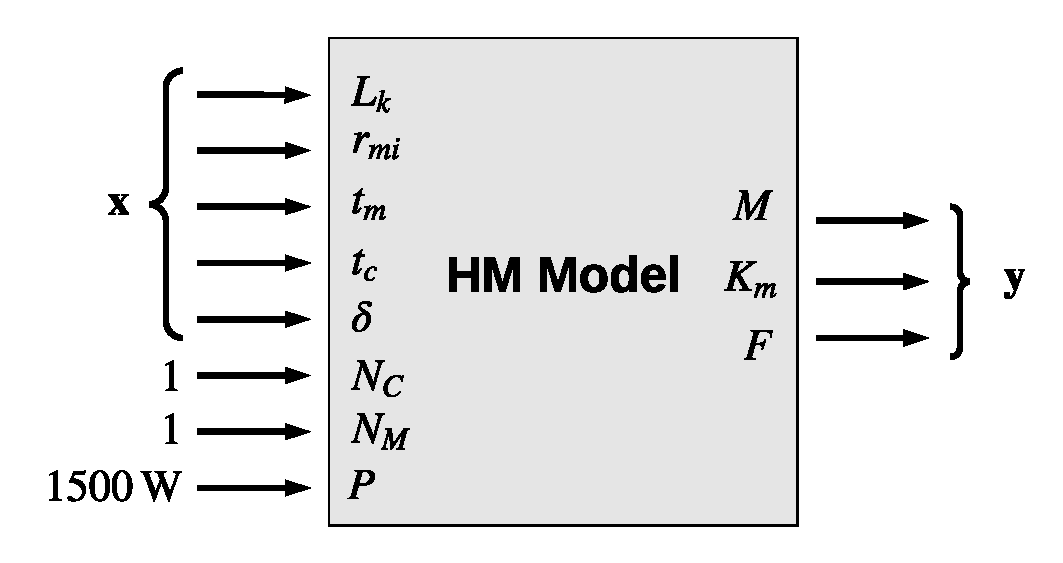
\includegraphics[width=4in]{chap4/images/HM_mining_for_PMLSM.pdf}
                \caption{A re-usable function to obtain \acs{RSM} training data based on \ac{HM} calculations of \ac{PMLSM}.}
                \label{fig:chapter/rsm/PMLSM/mining process}
            \end{figure}
            
            
            The $103680$ input cases were queried against a re-usable function as illustrated in Fig.\,\ref{fig:chapter/rsm/PMLSM/mining process} to obtain the corresponding outputs for each input set. The necessary information was then reduced back to a table that captured the motor design parameters in CSV format. 
            
        
        % -----------------------------------------------------------------------------------
        % --- NEW SUB SECTION --- NEW SUB SECTION --- NEW SUB SECTION --- NEW SUB SECTION --- 
        % -----------------------------------------------------------------------------------
        \subsection{Deep regression ANN training}   \label{Chapter:RSM/PMLSM/ANN training}
        
            
            Deep learning belongs to a broader family of machine learning methods which is very useful in capturing complex non-linear patterns with almost any data set. The data set is required to provide both the continuous input variables (structural design factors), and the continuous output variable (thrust characteristics at a given power). The classification of this application is a supervised and regression type of machine learning problem.
            
            
            Because some design parameters ($gap_{mc}$, $gap_{cf}$, $P$ and others) were established with constant values, the \acs{ANN} do not need to include them into the Input Layer. On the other hand, including both the thrust $F$ and the motor constant $K_m$ will introduce unwanted redundancy for a fixed power $P$ study. Therefore, only the motor constant $K_m$ was included in the model prediction. Three \acs{ANN} models were implemented and trained using Keras and Tensorflow machine learning frameworks:
            
            
            \begin{itemize}
                \item $5$ structural parameters were regarded as the Input Layer: $L_k$,$r_{mi}$, $t_m$, $t_c$, and $\delta$,
                \item $1$ performance output was regarded as the Output Layer: $K_m$,
                \item The optimizer for training the \acs{ANN} was the Adam optimizer,
                \item $6$ hidden layers of densely connected nodes: $256-512-512-512-512-512$ nodes for each layer,
                \item The rectified linear unit (ReLU) activation function was used
for the input and hidden layer,
                \item The linear activation function was used for the output layer,
                \item The error to optimize for was \acf{MSE},
                \item The training and validation split chosen at random for each of the three models were: $70\%-30\%$, $75\%-25\%$, and $80\%-20\%$,
                The final \acs{ANN} model was ensembled from the average of three models above.
            \end{itemize}
            
            
            \begin{figure*}[!ht]
                \centering
                \subfloat[$70\%-30\%$ split model
                ]{
                    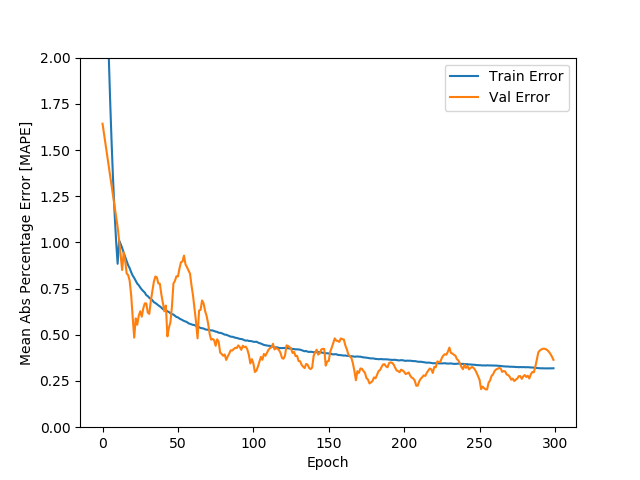
\includegraphics[width=0.5\textwidth]{chap4/images/MAPE_MSE_6_70-30_SPLIT.png}
                    \label{fig:chapter/rsm/PMLSM/training result/MAPE_70_30}
                }
                \subfloat[$75\%-25\%$ split model
                ]{
                    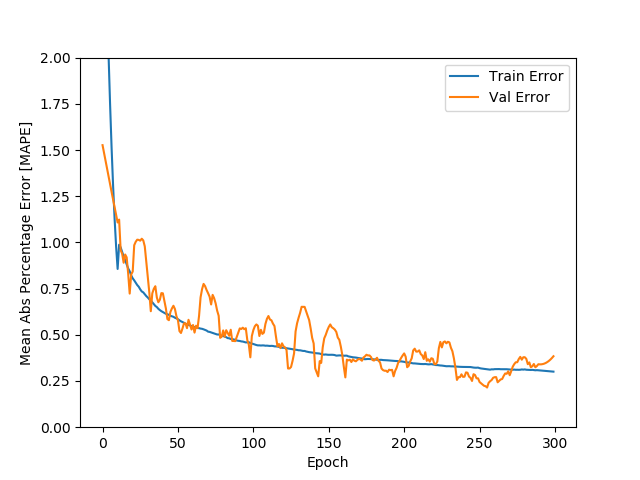
\includegraphics[width=0.5\textwidth]{chap4/images/MAPE_MSE_6_75-25_SPLIT.png}
                    \label{fig:chapter/rsm/PMLSM/training result/MAPE_75_25}
                }
                \\
                \subfloat[$80\%-20\%$ split model
                ]{
                    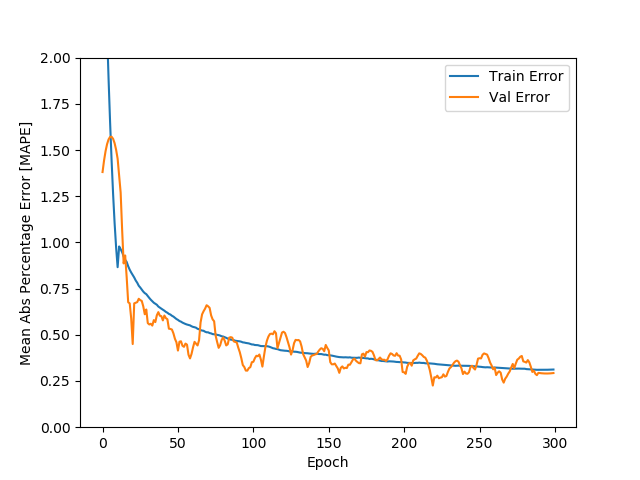
\includegraphics[width=0.5\textwidth]{chap4/images/MAPE_MSE_6_80-20_SPLIT.png}
                    \label{fig:chapter/rsm/PMLSM/training result/MAPE_80_20}
                }
                \caption{
                    Error produced by the deep learning \acs{ANN} model to represent \acsp{PMLSM}  vs. iterations for the training data (blue) and validation data (orange). The \acs{MAPE} is plotted for the training process of (a) $70\%-30\%$, (b) $75\%-25\%$, and (c) $80\%-20\%$ models, respectively.
                }   \label{fig:chapter/rsm/PMLSM/training result}
            \end{figure*}
            
            
            After $300$ training iterations, the models were shown to have an average \acf{MAPE} of $0.24\%$. The training and validation errors were similar, showing that the deep regression model was not over-fitted to the training data set. Fig.\,\ref{fig:chapter/rsm/PMLSM/training result} shows the training and validation error during the \acs{ANN} training process for each of the three models studied.
            
        
        % -----------------------------------------------------------------------------------
        % --- NEW SUB SECTION --- NEW SUB SECTION --- NEW SUB SECTION --- NEW SUB SECTION --- 
        % -----------------------------------------------------------------------------------
        \subsection{Optimization}                   \label{Chapter:RSM/PMLSM/Optimization}
        
        
            Following the outer and inner optimization setup in Section\,\ref{Chapter:PMLSM design HM/design optimization/optimization formulation}, the next step was to repeat the optimization run in Section\,\ref{Chapter:PMLSM design HM/benchmark study} with some differences. Instead of using the \acs{HM} equations as the mean estimate $K_m$ for the whole motor, the \acs{ANN} was employed to estimate the motor constant $K_m$ of a single repeat unit consisting of one half coil-phase ($N_C = 1$), and one half magnet-phase ($N_M = 1$). 
            
            
            During the execution of the optimization algorithm, many motors with half coil-phase values larger than $N_C = 1$ were calculated. As mentioned previously, the \acs{ANN} only estimate $K_m$ for motor units with $N_C=1$ and $N_M=1$. There requires a conversion for the motor constant of the whole motor $K_{m-whole}$, given that a new number of half coil-phase $N_{C-whole}$ that is larger than $1$:
            
            
            \begin{equation}
                K_{m-whole}=K_m  \sqrt{N_{C-whole}}
                \label{eq:calculate new K_m based on new N_C}
            \end{equation}
            
            
            Adapting to this change, the maximum jet velocity $v_{jet}$ becomes:
            
            
            \begin{equation}
                v_{jet} = \sqrt[4]{\frac{4P {K_{m-whole}}^2 {L_S}^2}{\rho_w V^2}}
                \label{eq:calculate new v_jet based on new N_C}
            \end{equation}
            
            
            Except when it comes to collecting the motor mass $M$, Equation\,\ref{eq:mass of motor via mass dimless} was borrowed from the \acs{HM} electromagnetic calculation. 
            
            
            \begin{figure*}[!ht]
                \par\bigskip
                \centering
                \subfloat[Sub-routine setup: Each objective function evaluation will start a separate sub-routine, taking roughly $6$ seconds.]{
                    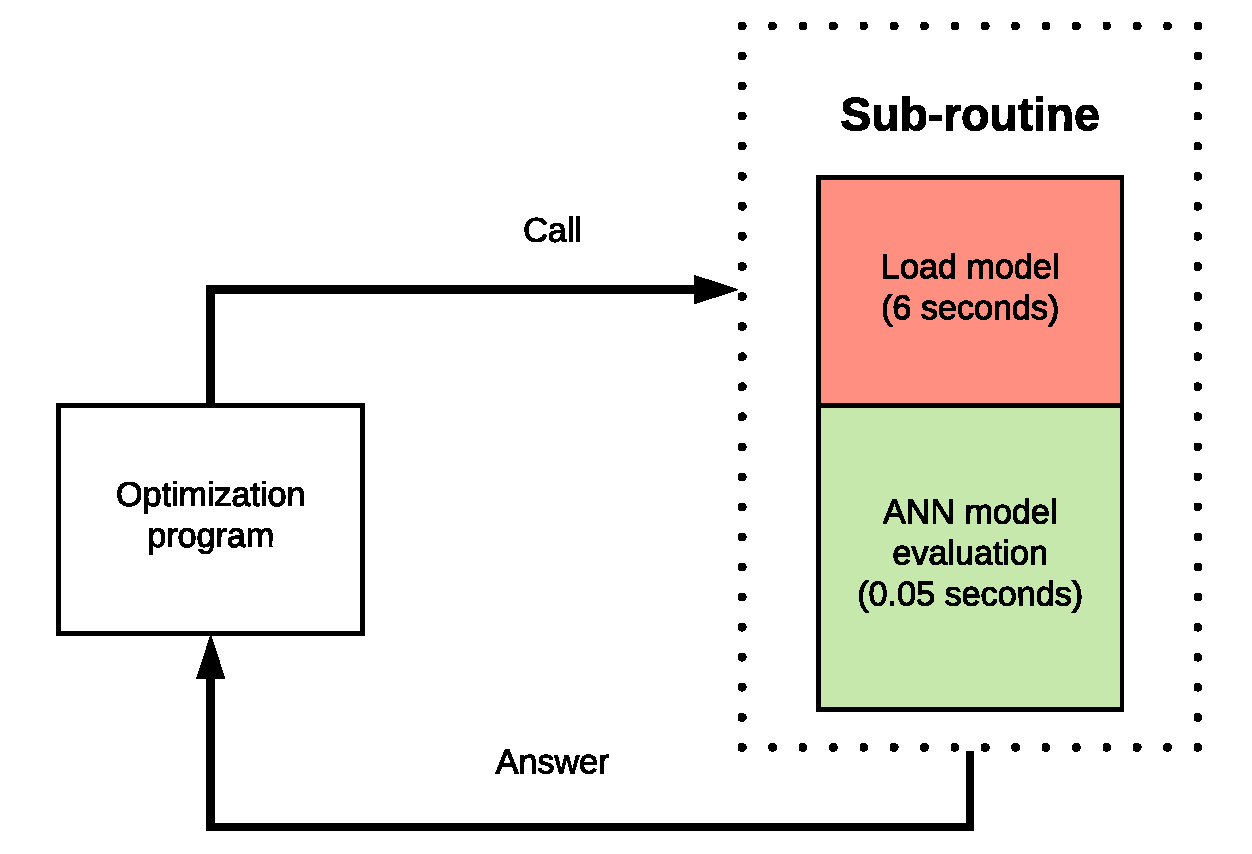
\includegraphics[width=0.45\textwidth]{chap4/images/inference_routine.pdf}
                    \label{fig:chapter/rsm/PMLSM/inference options/routine}
                }
                \,\,\,\,\,\,
                \subfloat[Web-server setup: The model is loaded only once, and all objective function evaluations take less than $0.05$ seconds.]{
                    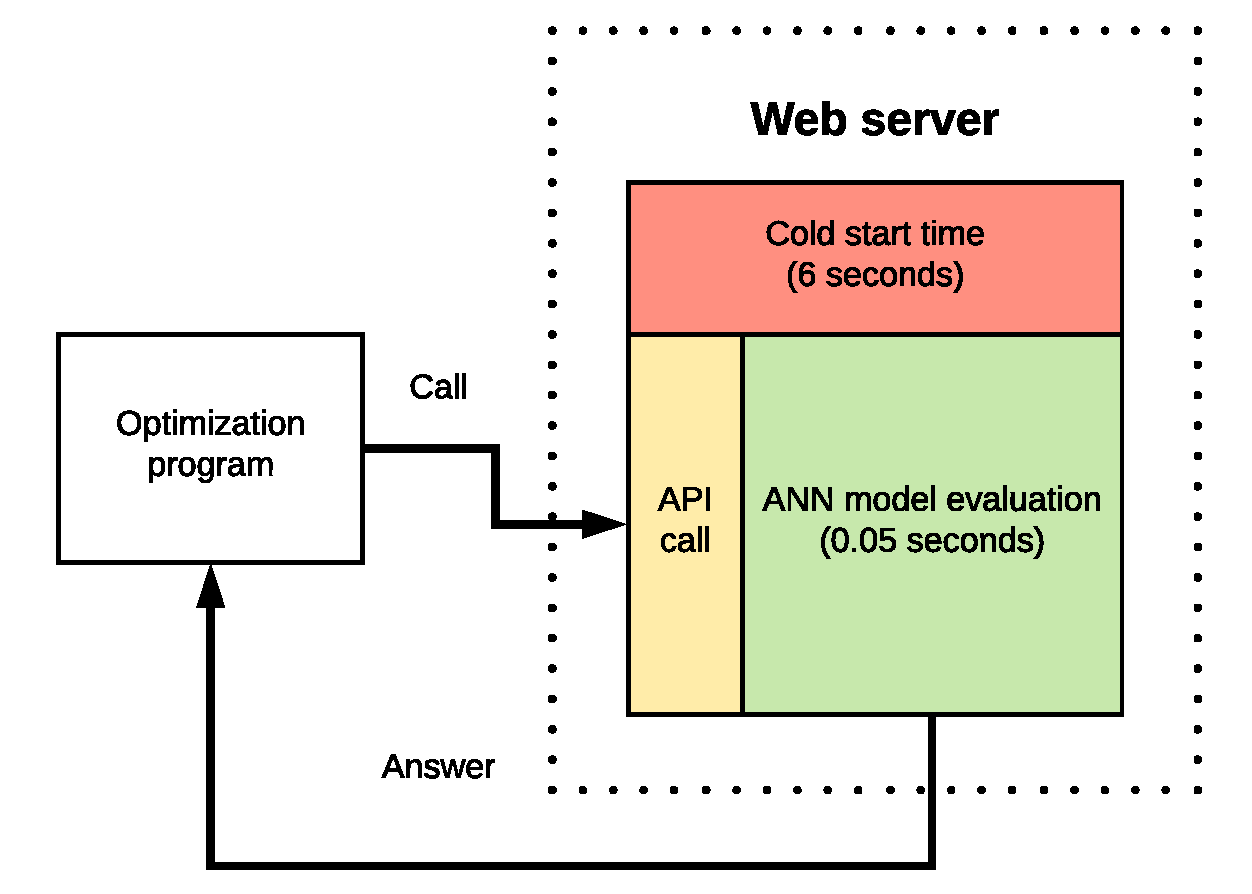
\includegraphics[width=0.45\textwidth]{chap4/images/inference_web_services.pdf}
                    \label{fig:chapter/rsm/PMLSM/inference options/web services}
                }
                \caption{
                    Two different styles of optimization objective function evaluation.
                }\label{fig:chapter/rsm/PMLSM/inference options}
            \end{figure*}
            
            
            In the normal circumstances, a full execution cycle for inferring the \acs{ANN} model includes waiting for the model to load, querying the model, then terminating the model until the next execution. However, loading the \acs{ANN} model in the Python environment may take a few seconds, the result is that numerous inferences of the existing model made by the optimization algorithm would cost an enormous amount of time. Alternatively, the optimization objective function evaluation should interact with the trained \acs{ANN} model in the fashion of a web server instead of a sub-routine, as illustrated in Fig.\,\ref{fig:chapter/rsm/PMLSM/inference options}.


        % -----------------------------------------------------------------------------------
        % --- NEW SUB SECTION --- NEW SUB SECTION --- NEW SUB SECTION --- NEW SUB SECTION --- 
        % -----------------------------------------------------------------------------------
        \subsection{Results}                   \label{Chapter:RSM/PMLSM/Results}


            With the objective function evaluation using \acs{ANN} models at its core, the global optimization of \acs{PMLSM} for the problem described in Equation\,\ref{eq:outer optimization for PMLSMs} is summarized in Table\,\ref{table:result for global optimization of PMLSM via RSM method}. The table shows the optimization results for different motor mass constraints $M_0=[325,350,375,400,425]\,\mathrm{g}$.
            
            
            For instance, the global optimization for the constraints set $P=1500\,\mathrm{W}$, $V=1\,\mathrm{mL}$, $gap_{mc}=1.2\,\mathrm{mm}$, $gap_{cf}=0.1\,\mathrm{mm}$, $M_0=325\,\mathrm{g}$ on the search space of $L_{M0}:120\,\mathrm{mm}\rightarrow 160\,\mathrm{mm} \times L_{C0}:50\,\mathrm{mm}\rightarrow 90\,\mathrm{mm}$, the optimization program found an under-hung motor with $N_C=4$, $N_M=12$, $L_k=26.5\,\mathrm{mm}$, $r_{mi}=2\,\mathrm{mm}$, $t_m=6.15\,\mathrm{mm}$, $t_c=3\,\mathrm{mm}$, $\delta=0.30$. This motor configuration is able to theoretically produce $246.45\,\mathrm{N}$ at the rated power, which corresponds to a motor constant $K_m=6.36\,\mathrm{N/\sqrt{W}}$ and a peak jet speed $v_{jet}=228.67\,\mathrm{m/s}$. Table\,\ref{table:result for global optimization of PMLSM via HM method} shows that the same optimization problem powered by \acs{HM} electromagnetic equations produced almost exactly the same results when compared with \acs{RSM} method. The \acs{RSM} method predicted the peak jet speed $v_{jet}=228.67\,\mathrm{mm}$ while the \acs{HM} method predicted $v_{jet}=228.92\,\mathrm{mm}$. The only difference was the value of the ratio $\delta$ which does not affect the motor mass $M$.  
            
            
            Fig.\,\ref{fig:chapter/rsm/PMLSM/results} provides global optimization plots of $v_{jet}$ for the search space $L_{M0}:120\,\mathrm{mm}\rightarrow 160\,\mathrm{mm} \times L_{C0}:50\,\mathrm{mm}\rightarrow 90\,\mathrm{mm}$ using $P=1500\,\mathrm{W}$, $V=1\,\mathrm{mL}$, $gap_{mc}=1.2\,\mathrm{mm}$, $gap_{cf}=0.1\,\mathrm{mm}$,  and $M_0=[325,350,375,400,425]\,\mathrm{g}$. Not only do the global optimization results obtained by different modelling methods agreed strongly, the contour plots populated by the optimization processes of \acs{RSM} (Fig.\,\ref{fig:chapter/rsm/PMLSM/results}) and \acs{HM} (Fig.\,\ref{fig:chapter/hm/optimization search space result for differnt mass}) looked almost identical. This study successfully demonstrated the effectiveness and the accuracy of design and optimization process presented in Section\,\ref{Chapter:RSM/outline}.
        

            
            \begin{landscape}
                \begin{table}
                    \renewcommand{\arraystretch}{1.2}
                    \caption{Summary of motor design optimization values and performance using \acs{RSM} method}
                    \label{table:result for global optimization of PMLSM via RSM method}
                    \centering
                    \begin{tabular}{lllrrrrr}
                        \hline
                        \textbf{Params}     & \textbf{Description}                            & \textbf{Unit}           & $M_0=\mathbf{325\,g}$ & $\mathbf{350\,g}$ & $\mathbf{375\,g}$ & $\mathbf{400\,g}$ & $\mathbf{425\,g}$ \\
                        \hline
                        $P$        & Power dissipation in coil winding      & $\mathrm{kW}$  & $1.50$                & $1.50$            & $1.50$            & $1.50$            & $1.50$            \\
                        $V$        & Volume of ampoule                      & $\mathrm{mL}$  & $1.00$                & $1.00$            & $1.00$            & $1.00$            & $1.00$            \\
                        $gap_{mc}$ & Magnet and coil fixed gap              & $\mathrm{mm}$  & $1.20$                & $1.20$            & $1.20$            & $1.20$            & $1.20$            \\
                        $gap_{cf}$ & Coil and iron fixed gap                & $\mathrm{mm}$  & $0.10$                & $0.10$            & $0.10$            & $0.10$            & $0.10$            \\
                        \hline
                        $L_{C0:optim}$ & Constraint $L_C$ winding at global optimum & $\mathrm{mm}$        & $53.00$                       & $53.00$           & $53.00$           & $53.00$           & $53.00$           \\
                        $L_{M0:optim}$ & Constraint $L_C+L_S$ at global optimum        & $\mathrm{mm}$        & $160.00$                      & $160.00$          & $160.00$          & $160.00$          & $160.00$          \\
                        \hline
                        $r_{mi}$   & Magnet array inner radius              & $\mathrm{mm}$  & $2.00$                & $2.00$            & $2.00$            & $2.00$            & $2.00$            \\
                        $t_m$      & Magnet thickness                       & $\mathrm{mm}$  & $6.15$                & $6.35$            & $6.67$            & $6.99$            & $7.29$            \\
                        $t_c$      & Coil thickness                         & $\mathrm{mm}$  & $3.00$                & $3.00$            & $3.00$            & $3.00$            & $3.00$            \\
                        $\delta$   & Ratio of radial magnet vs. magnet pair &                & $0.32$                & $0.25$            & $0.25$            & $0.25$            & $0.27$            \\
                        $N_C$      & Number of half coil-poles              &                & $4$                   & $3$               & $3$               & $3$               & $3$               \\
                        $N_M$      & Number of half magnet-poles            &                & $12$                  & $9$               & $9$               & $9$               & $9$               \\
                        \hline
                        $t_f$      & Iron shell thickness                   & $\mathrm{mm}$  & $0.77$                        & $1.07$            & $1.12$            & $1.15$            & $1.19$    \\       
                        $L_k$      & Full pole length                       & $\mathrm{mm}$  & $26.50$               & $35.33$           & $35.33$           & $35.33$           & $35.33$           \\
                        $L_C$      & Length of coil array                   & $\mathrm{mm}$  & $53.00$               & $53.00$           & $53.00$           & $53.00$           & $53.00$           \\
                        $L_M$      & Length of magnet array                 & $\mathrm{mm}$  & $159.00$              & $159.00$          & $159.00$          & $159.00$          & $159.00$          \\
                        $L_S$      & Stroke length                          & $\mathrm{mm}$  & $106.00$              & $106.00$          & $106.00$          & $106.00$          & $106.00$          \\
                        \hline
                        $v_{jet}$  & Achievable jet speed                   & $\mathrm{m/s}$ & $228.64$              & $234.21$          & $239.81$          & $245.13$          & $250.10$         \\
                        $F$        & Force exerts on piston                 & $\mathrm{N}$         & $246.45$                      & $258.72$          & $271.35$          & $283.44$          & $295.06$          \\
                        $K_m$      & Motor constant                         & $\mathrm{N/\sqrt{W}}$ & $6.36$                        & $6.68$            & $7.01$            & $7.32$            & $7.62$           \\
                        \hline
                    \end{tabular}
                \end{table}
            \end{landscape}
            
            \begin{figure*}[!ht]
                \centering
                \subfloat[$M_0=325\,\mathrm{g}$. Global optimum found at $L_{C0}=53\,\mathrm{mm}$, $L_{C0}=160\,\mathrm{mm}$, $N_C=4$, and $N_M=12$.
                ]{
                    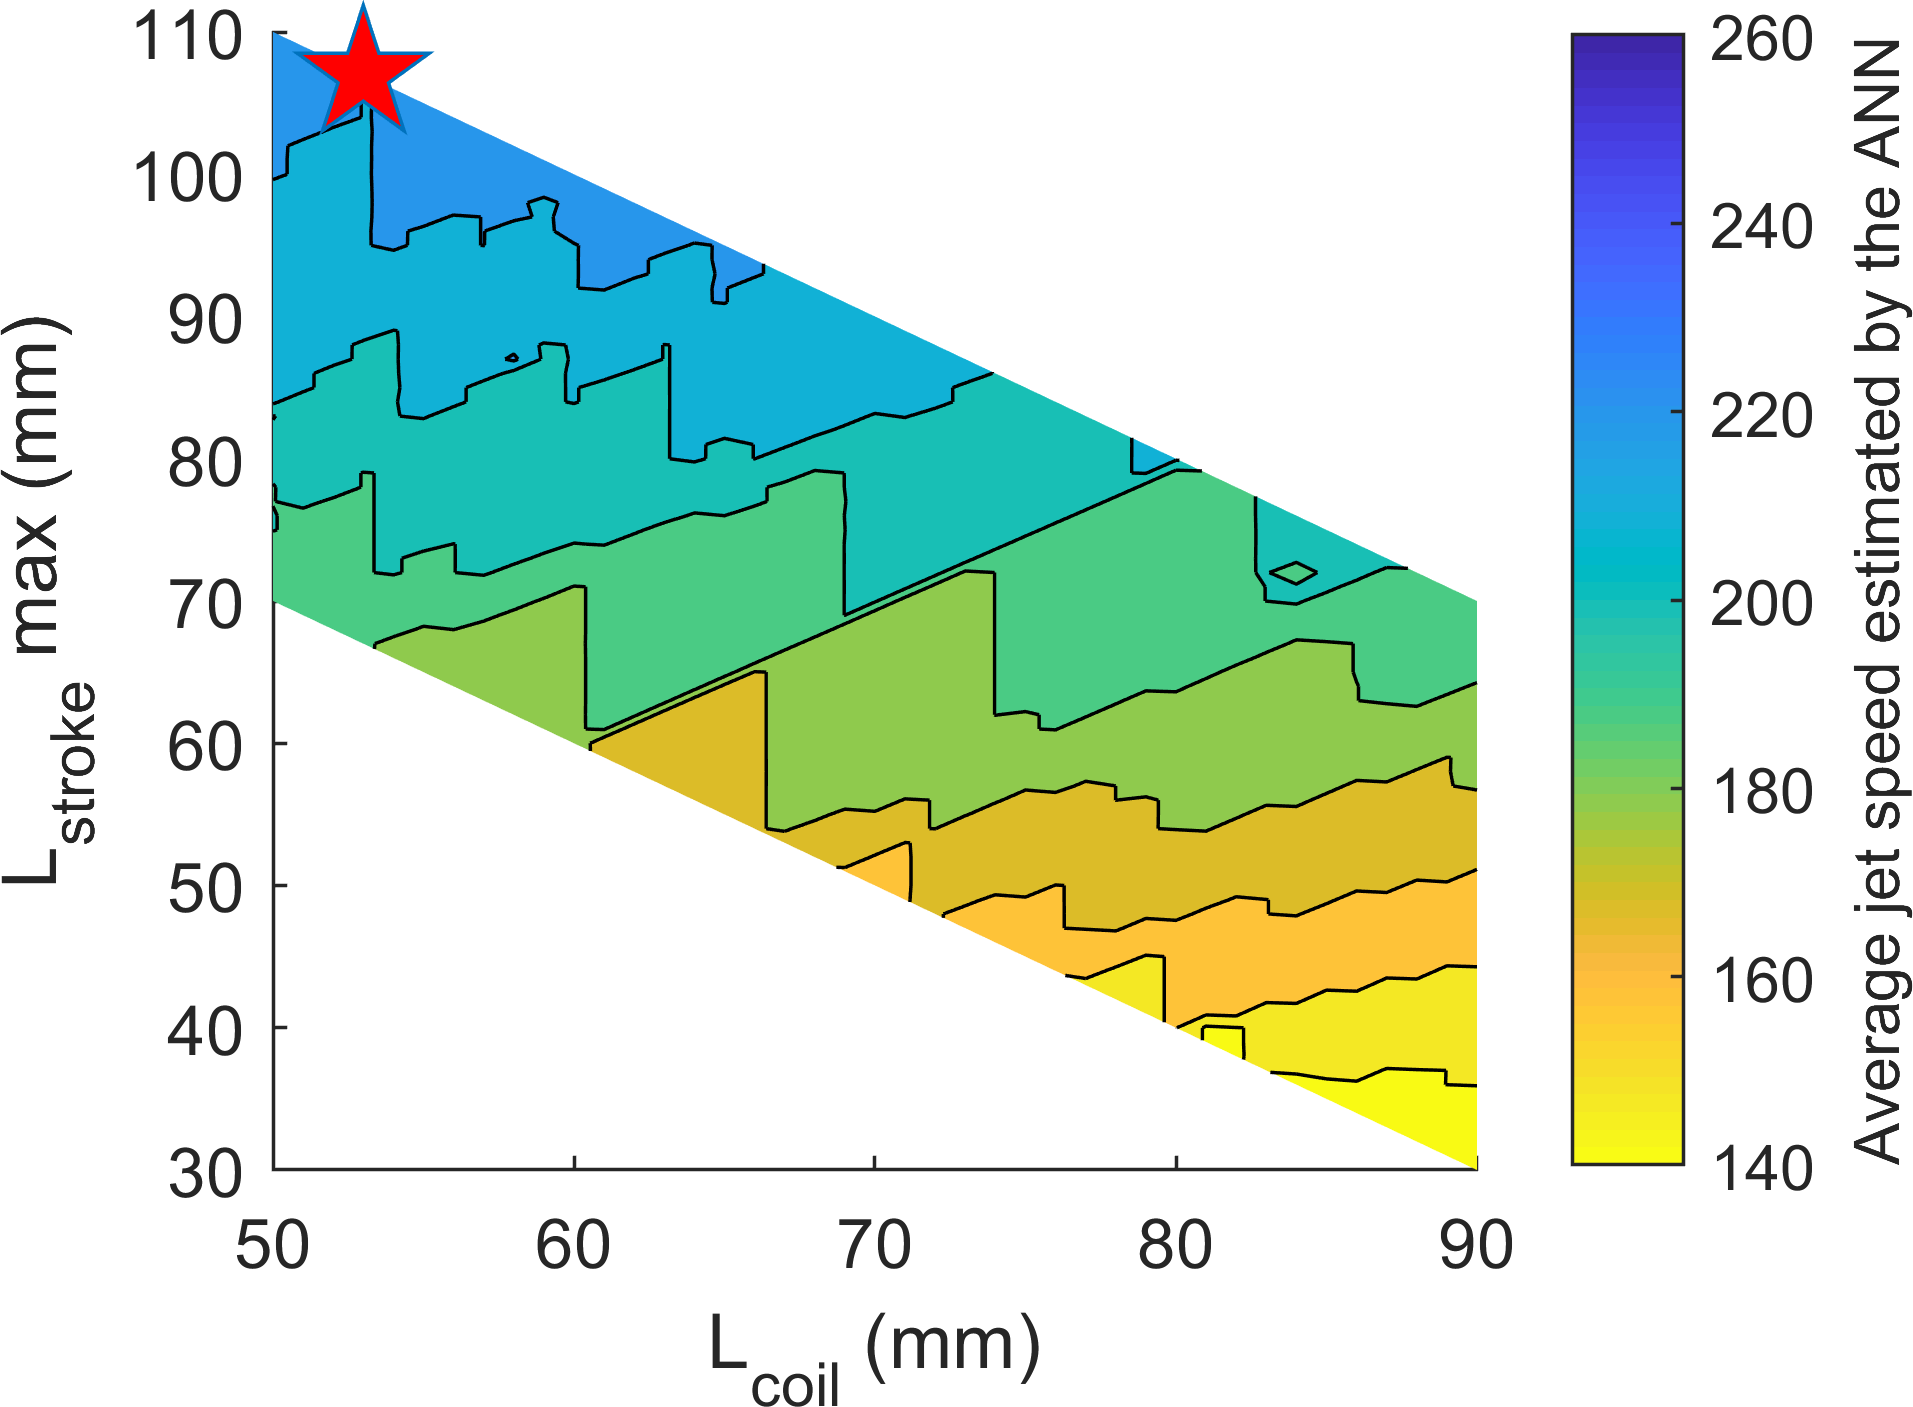
\includegraphics[width=0.45\textwidth]{chap4/images/PMLSM_RSM_325g.png}
                    \label{fig:chapter/rsm/PMLSM/results/325}
                }
                \qquad
                \subfloat[$M_0=350\,\mathrm{g}$ Global optimum found at $L_{C0}=53\,\mathrm{mm}$, $L_{C0}=160\,\mathrm{mm}$, $N_C=3$, and $N_M=9$.
                ]{
                    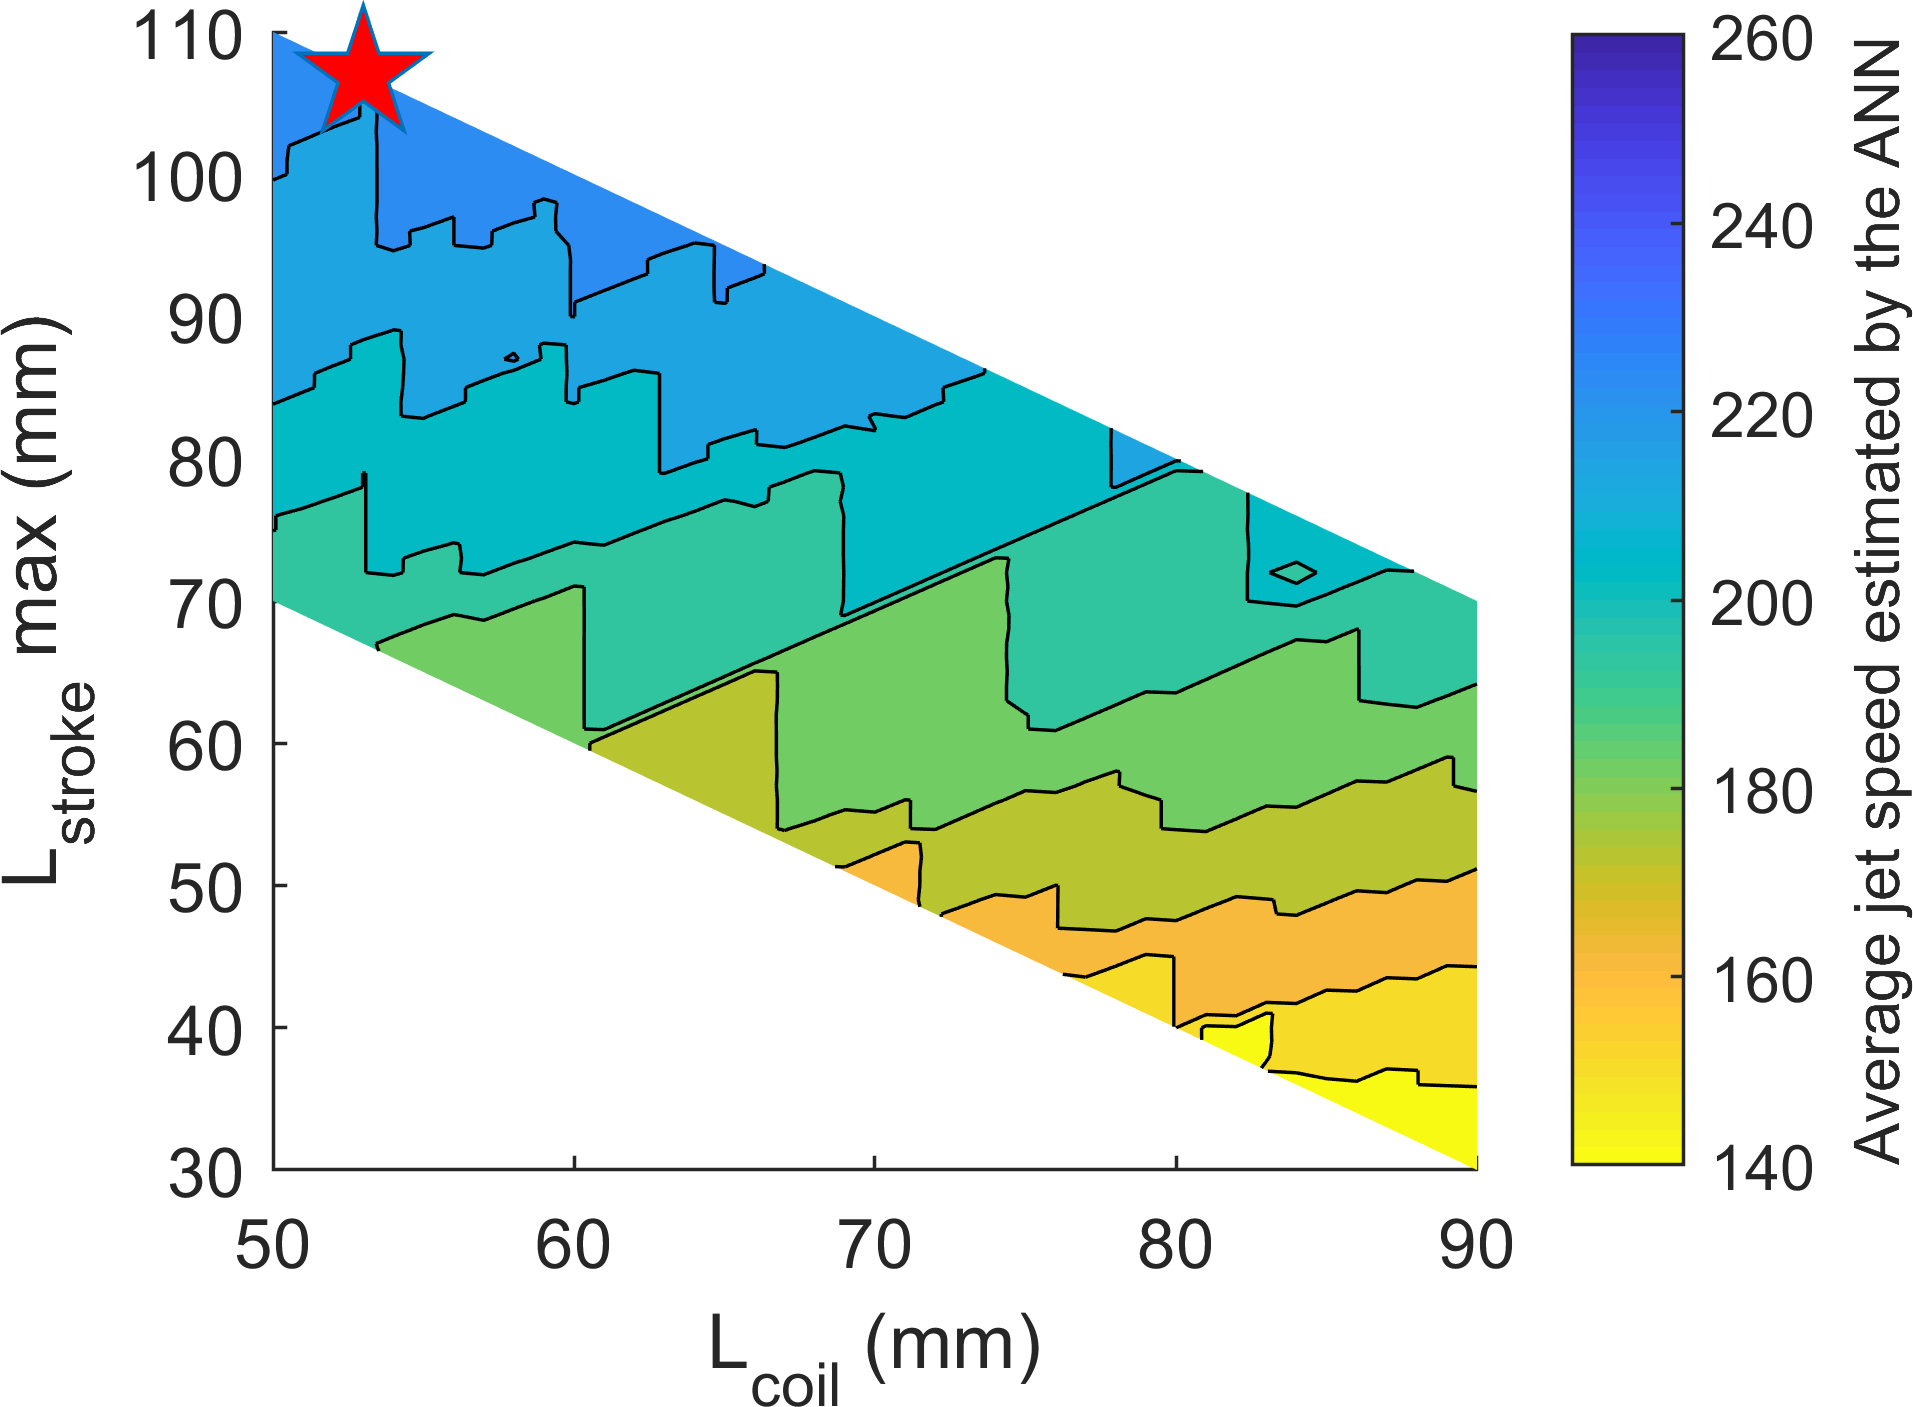
\includegraphics[width=0.45\textwidth]{chap4/images/PMLSM_RSM_350g.png}
                    \label{fig:chapter/rsm/PMLSM/results/350}
                }
                \\
                \subfloat[$M_0=375\,\mathrm{g}$. Global optimum found at $L_{C0}=53\,\mathrm{mm}$, $L_{C0}=160\,\mathrm{mm}$, $N_C=3$, and $N_M=9$.
                ]{
                    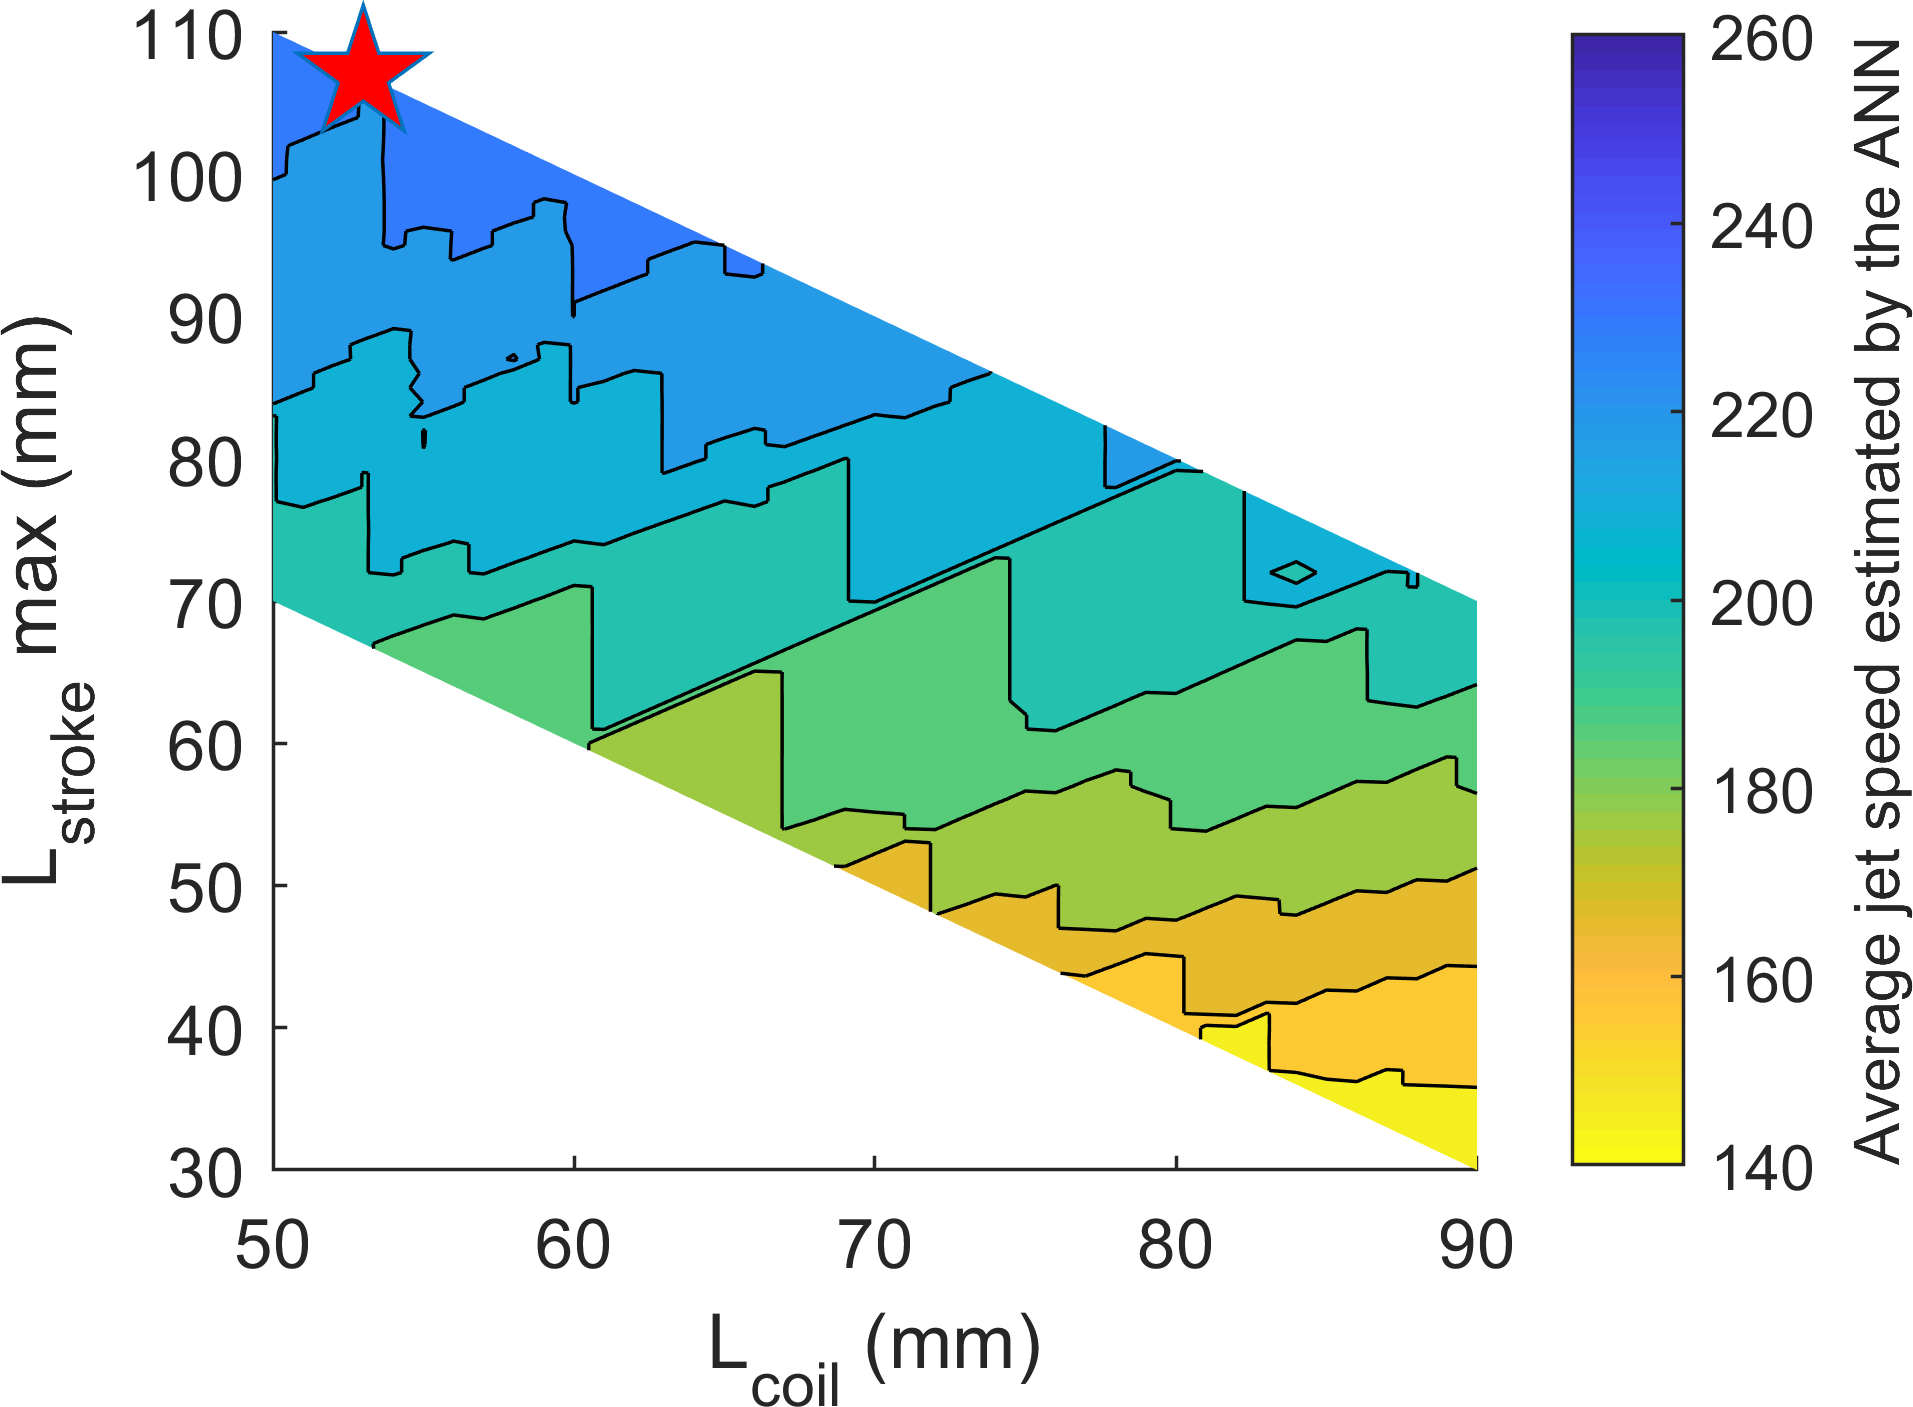
\includegraphics[width=0.45\textwidth]{chap4/images/PMLSM_RSM_375g.png}
                    \label{fig:chapter/rsm/PMLSM/results/375}
                }
                \qquad
                \subfloat[$M_0=400\,\mathrm{g}$. Global optimum found at $L_{C0}=53\,\mathrm{mm}$, $L_{C0}=160\,\mathrm{mm}$, $N_C=3$, and $N_M=9$.
                ]{
                    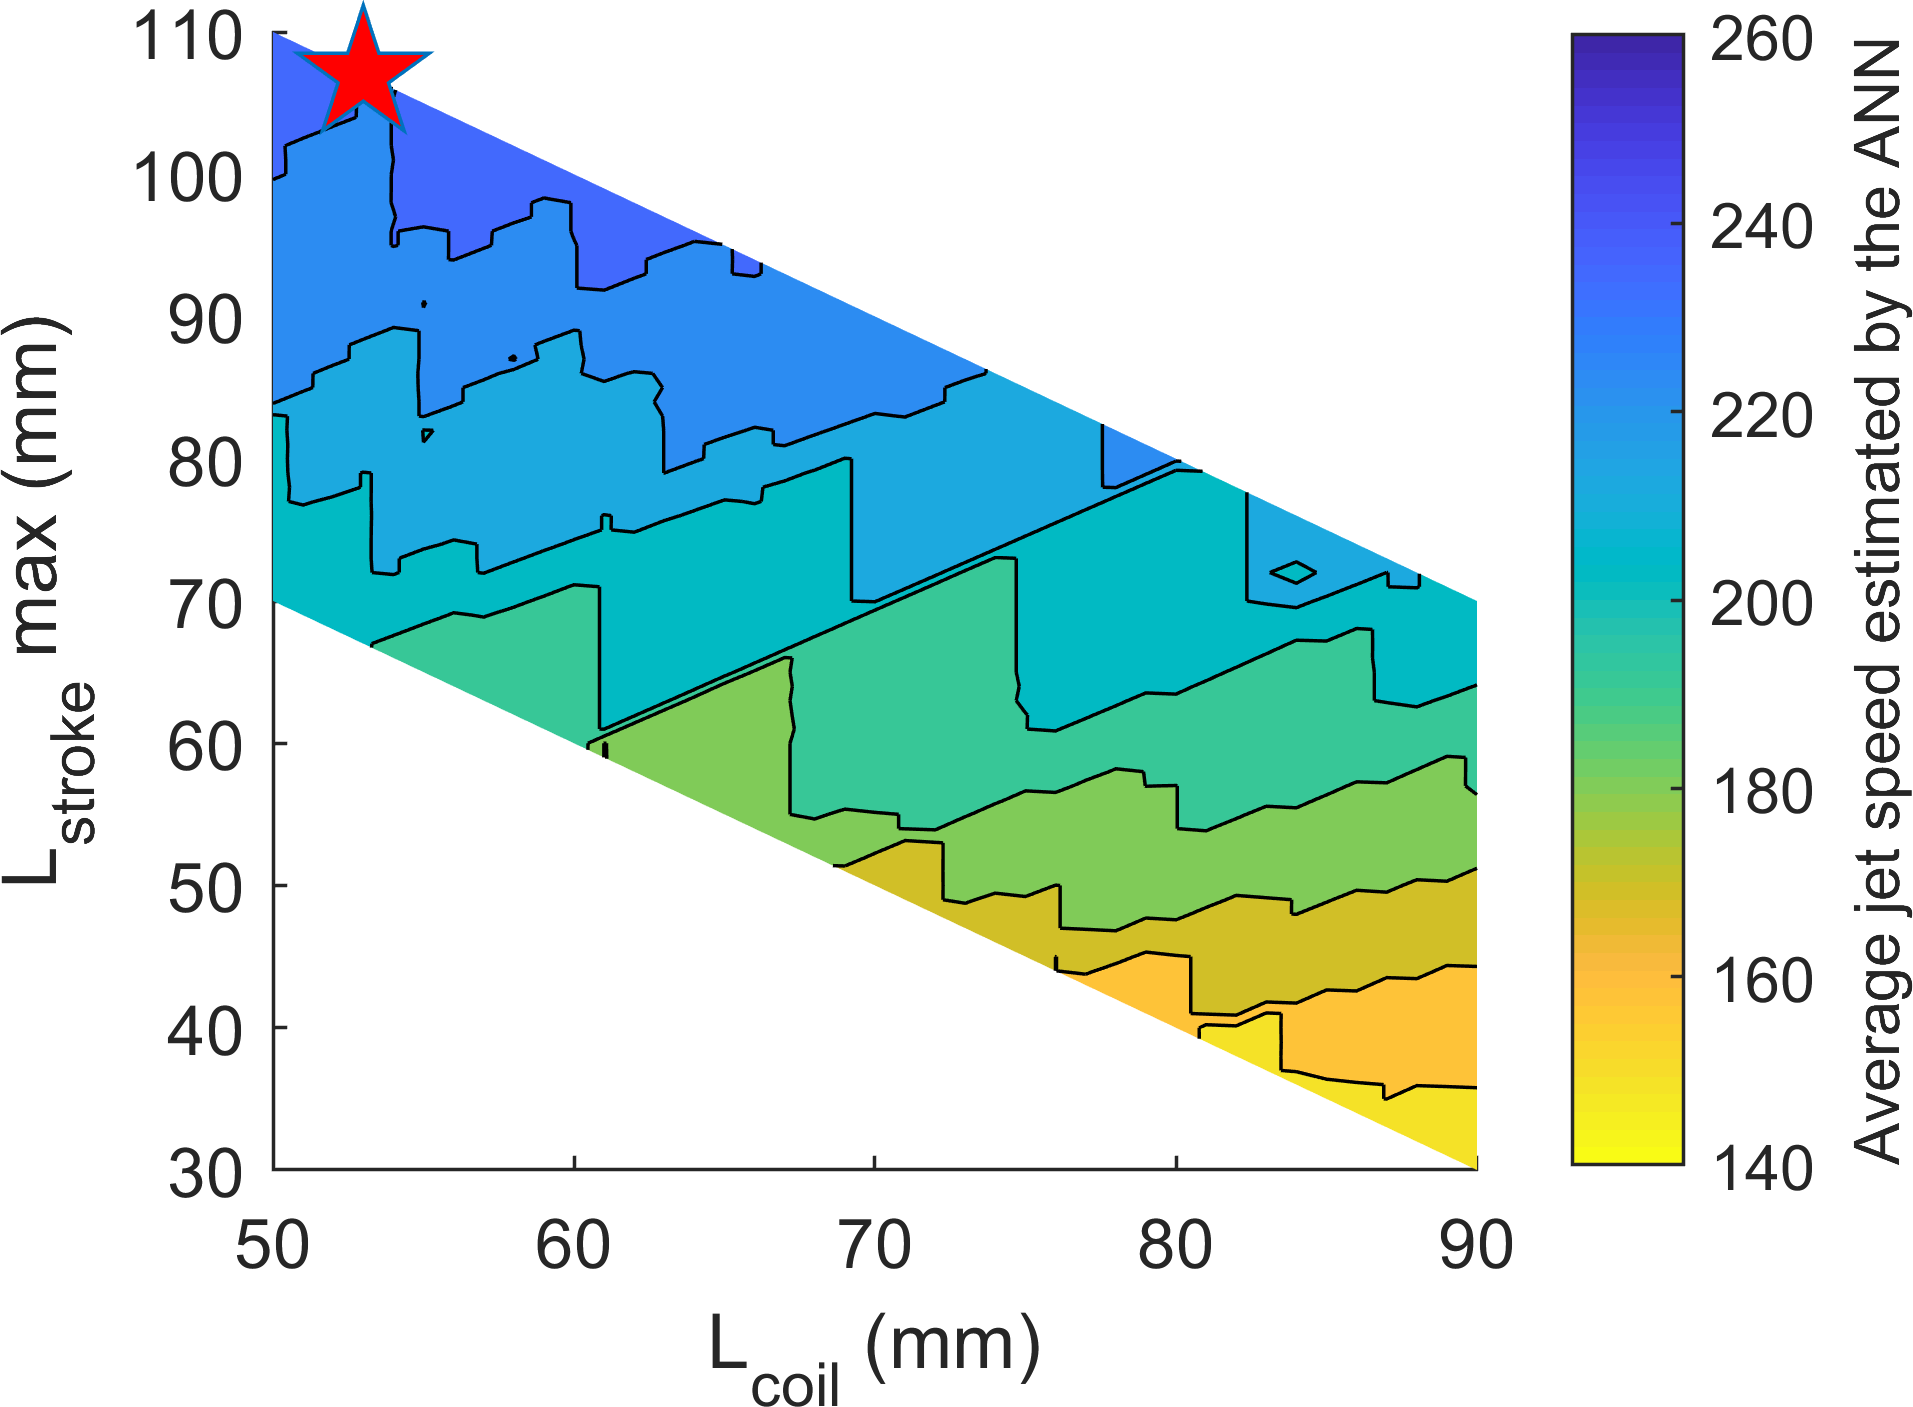
\includegraphics[width=0.45\textwidth]{chap4/images/PMLSM_RSM_400g.png}
                    \label{fig:chapter/rsm/PMLSM/results/400}
                }
                \\
                \subfloat[$M_0=425\,\mathrm{g}$. Global optimum found at $L_{C0}=53\,\mathrm{mm}$, $L_{C0}=160\,\mathrm{mm}$, $N_C=3$, and $N_M=9$.
                ]{
                    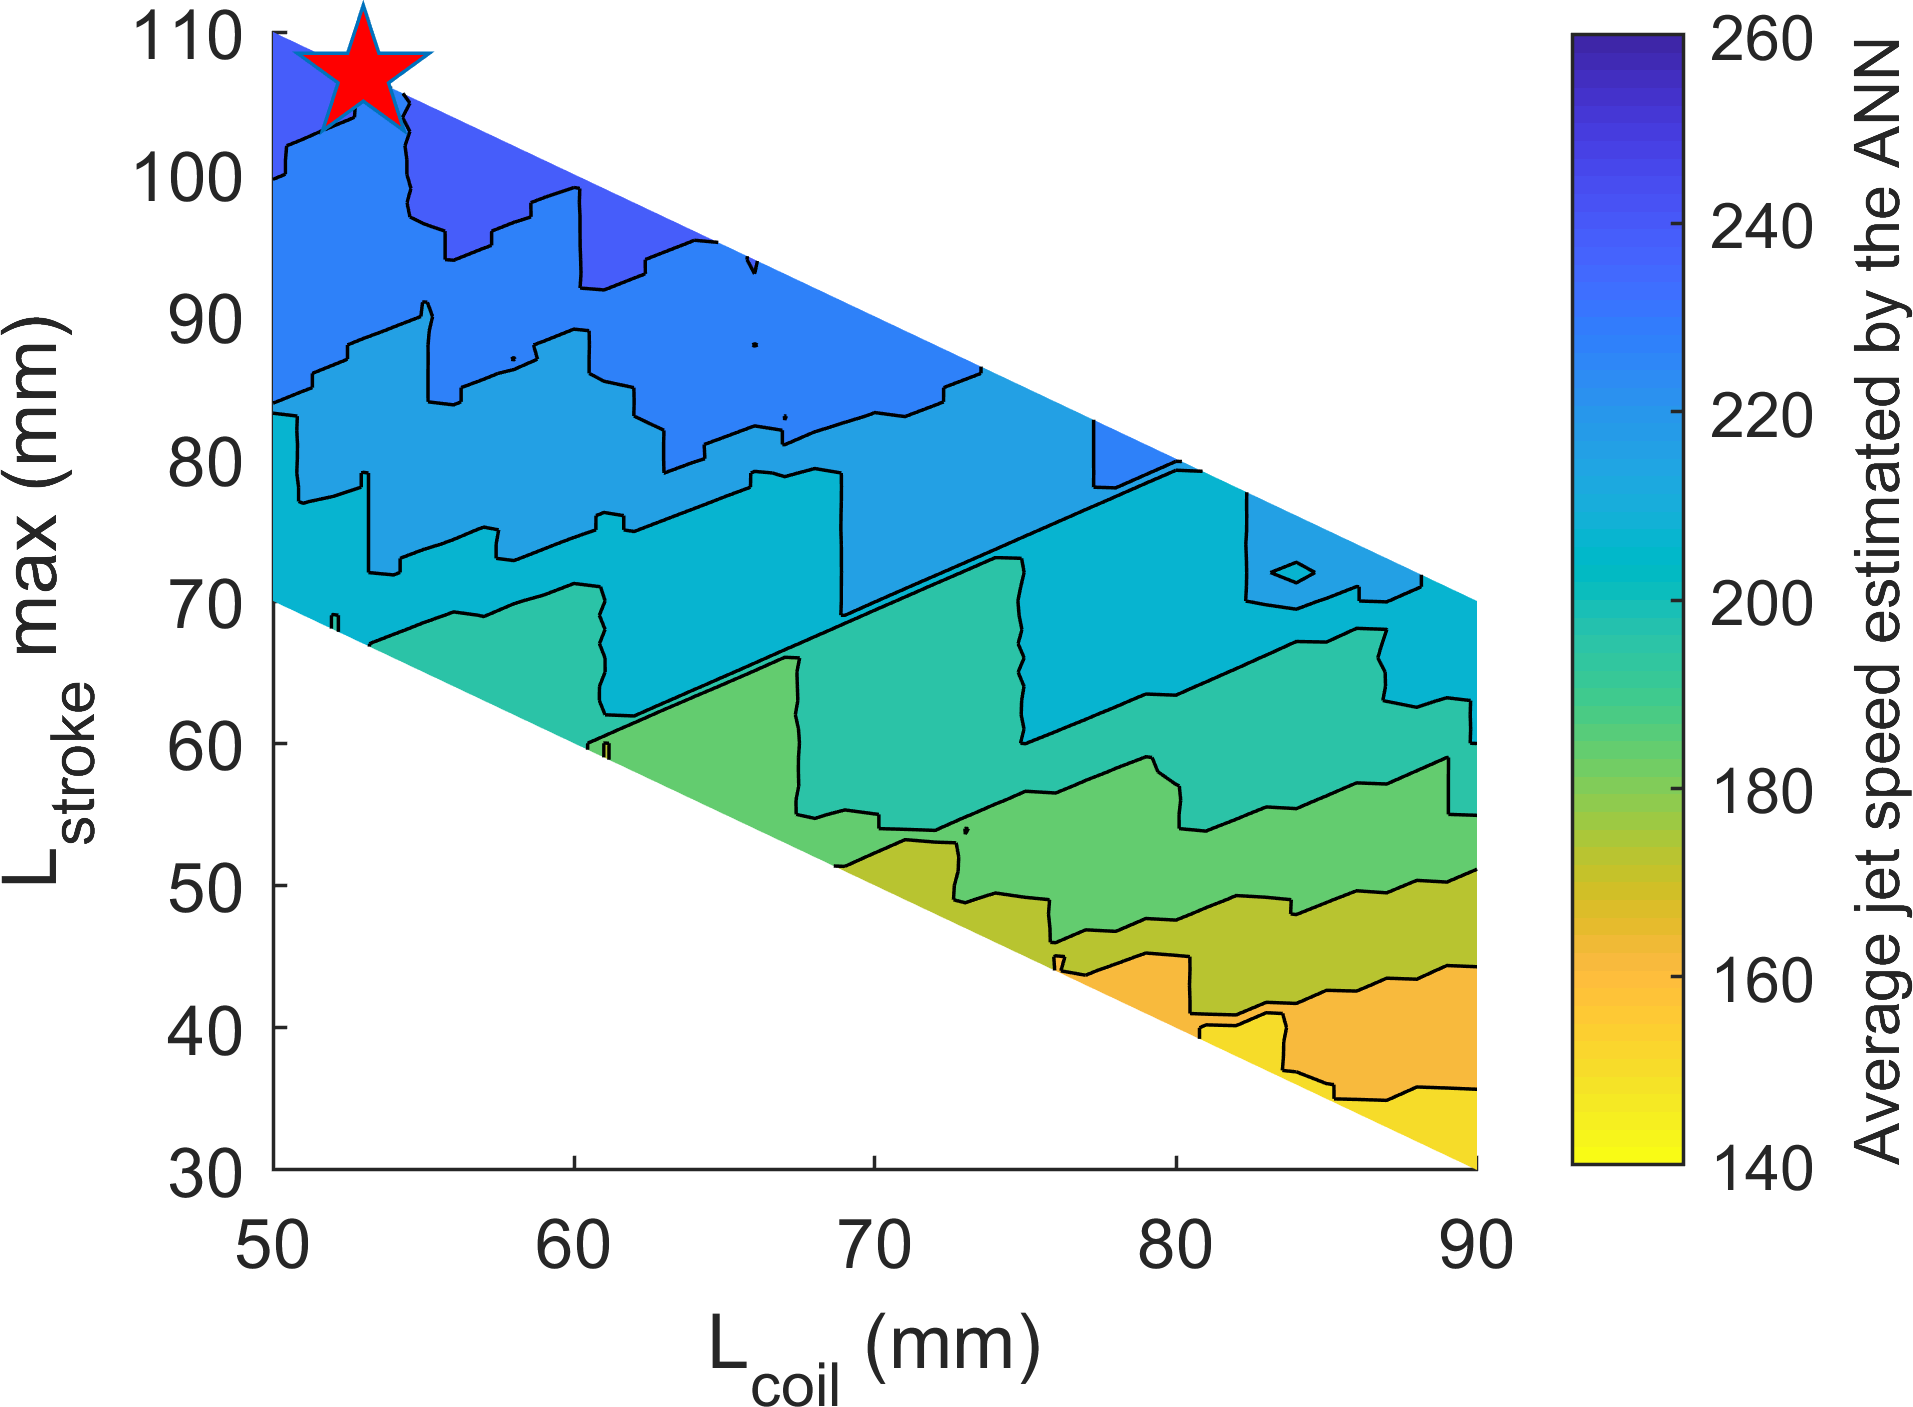
\includegraphics[width=0.45\textwidth]{chap4/images/PMLSM_RSM_425g.png}
                    \label{fig:chapter/rsm/PMLSM/results/425}
                }
                \\
                \caption{
                    The global optimization plots of $v_{jet}$ for the search space $L_{M0}:120\,\mathrm{mm}\rightarrow 160\,\mathrm{mm} \times L_{C0}:50\,\mathrm{mm}\rightarrow 90\,\mathrm{mm}$ using $P=1500\,\mathrm{W}$, $V=1\,\mathrm{mL}$, $gap_{mc}=1.2\,\mathrm{mm}$, $gap_{cf}=0.1\,\mathrm{mm}$,  and $M_0$ of: (a) $325\,\mathrm{g}$, (b) $350\,\mathrm{g}$, (c) $375\,\mathrm{g}$, (d) $400\,\mathrm{g}$, and (e) $425\,\mathrm{g}$.
                }   \label{fig:chapter/rsm/PMLSM/results}
            \end{figure*}
    
    % ===================================================================================================
    % === NEW SECTION === NEW SECTION === NEW SECTION === NEW SECTION === NEW SECTION === NEW SECTION ===
    % ===================================================================================================
    \section{Application to \ac{LFSM}}               \label{Chapter:RSM/LFSM}
    
    
        This study attempts to clarify the performance characteristics of \acsp{LFSM} when applied to \acs{NFJI} applications. The C-core topology was the most favourable, because they typically produce more thrust than E-core topologies \cite{Min2011OptimizationMachines}. A conventional 6 slot/5 pole \acs{LFSM} as shown in Fig.\,\ref{fig:chapter/rsm/LFSM/structure/6-5} has minimal thrust ripple due to cancellation of even order and third order harmonics. However, this work chose to study a 6 slot/7 pole LFSM structure as illustrated  in Fig.\,\ref{fig:chapter/rsm/LFSM/structure/6-7} because it is reported to also produce more thrust than other configurations, even though it may come at the expense of having more thrust ripple \cite{Chen2010}. 
        
        
        \begin{figure*}[!ht]
            \centering
            \subfloat[\label{fig:chapter/rsm/LFSM/structure/6-7}Tubular LFSM with 6 slots and 7 poles per period.]{
                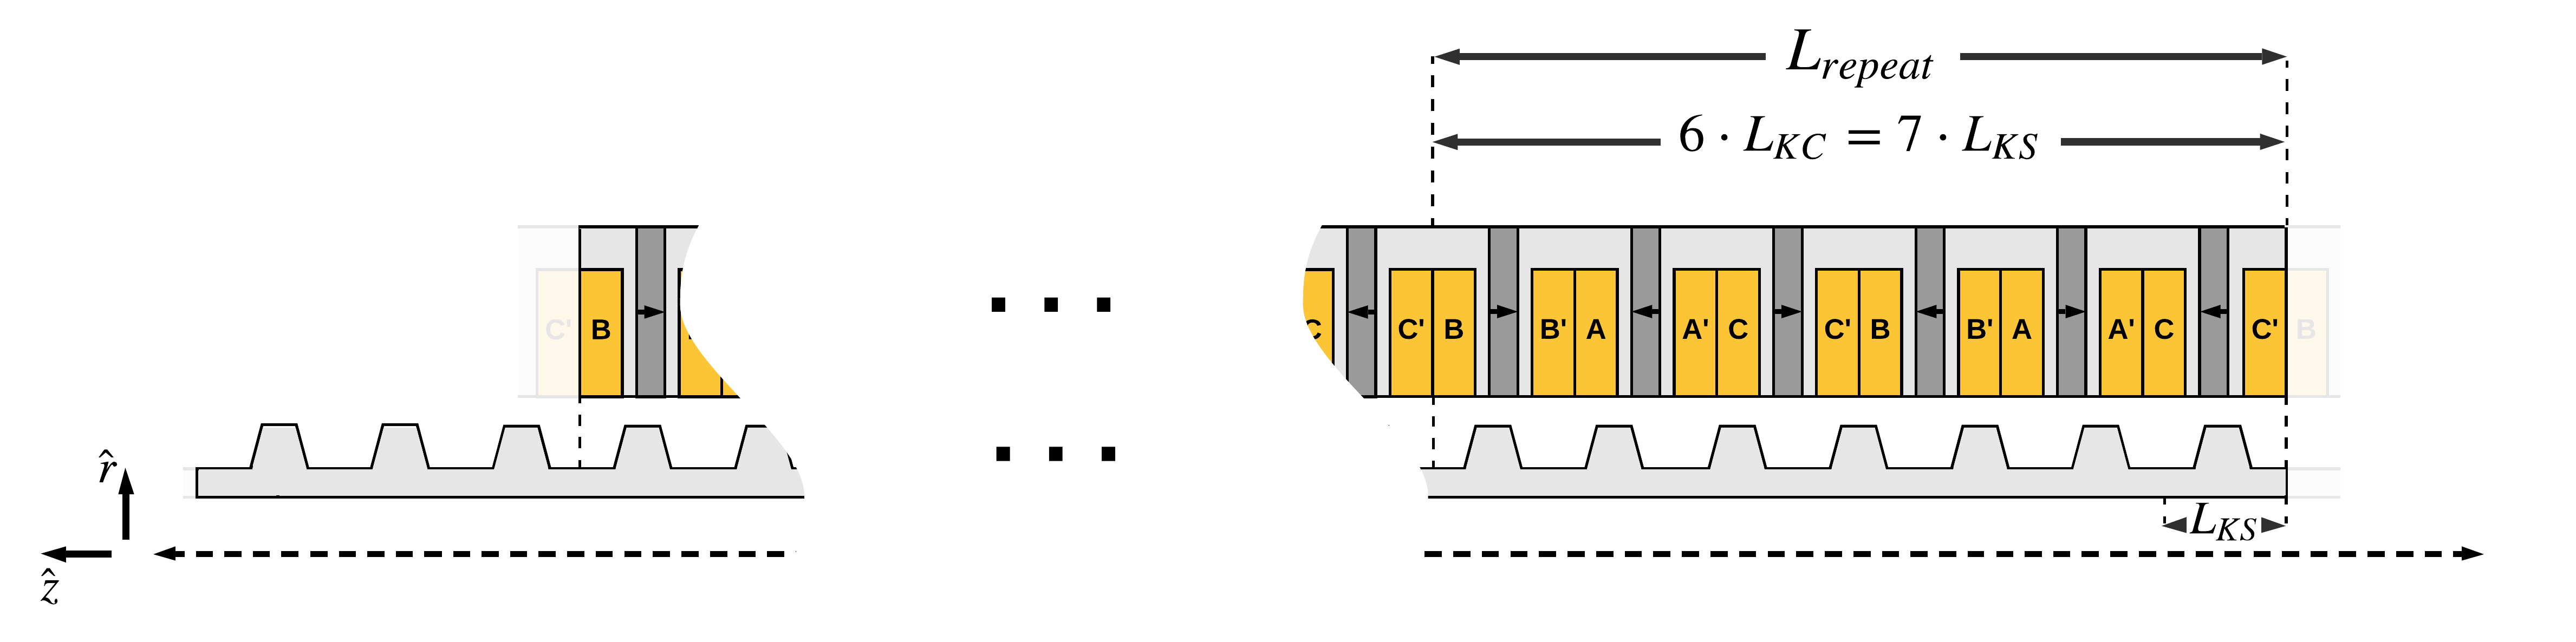
\includegraphics[width=0.97\textwidth]{chap4/images2/LFSM_6_7.png}
            }
            \\
            \subfloat[\label{fig:chapter/rsm/LFSM/structure/6-5}Tubular LFSM with 6 slots and 5 poles per period.]{
                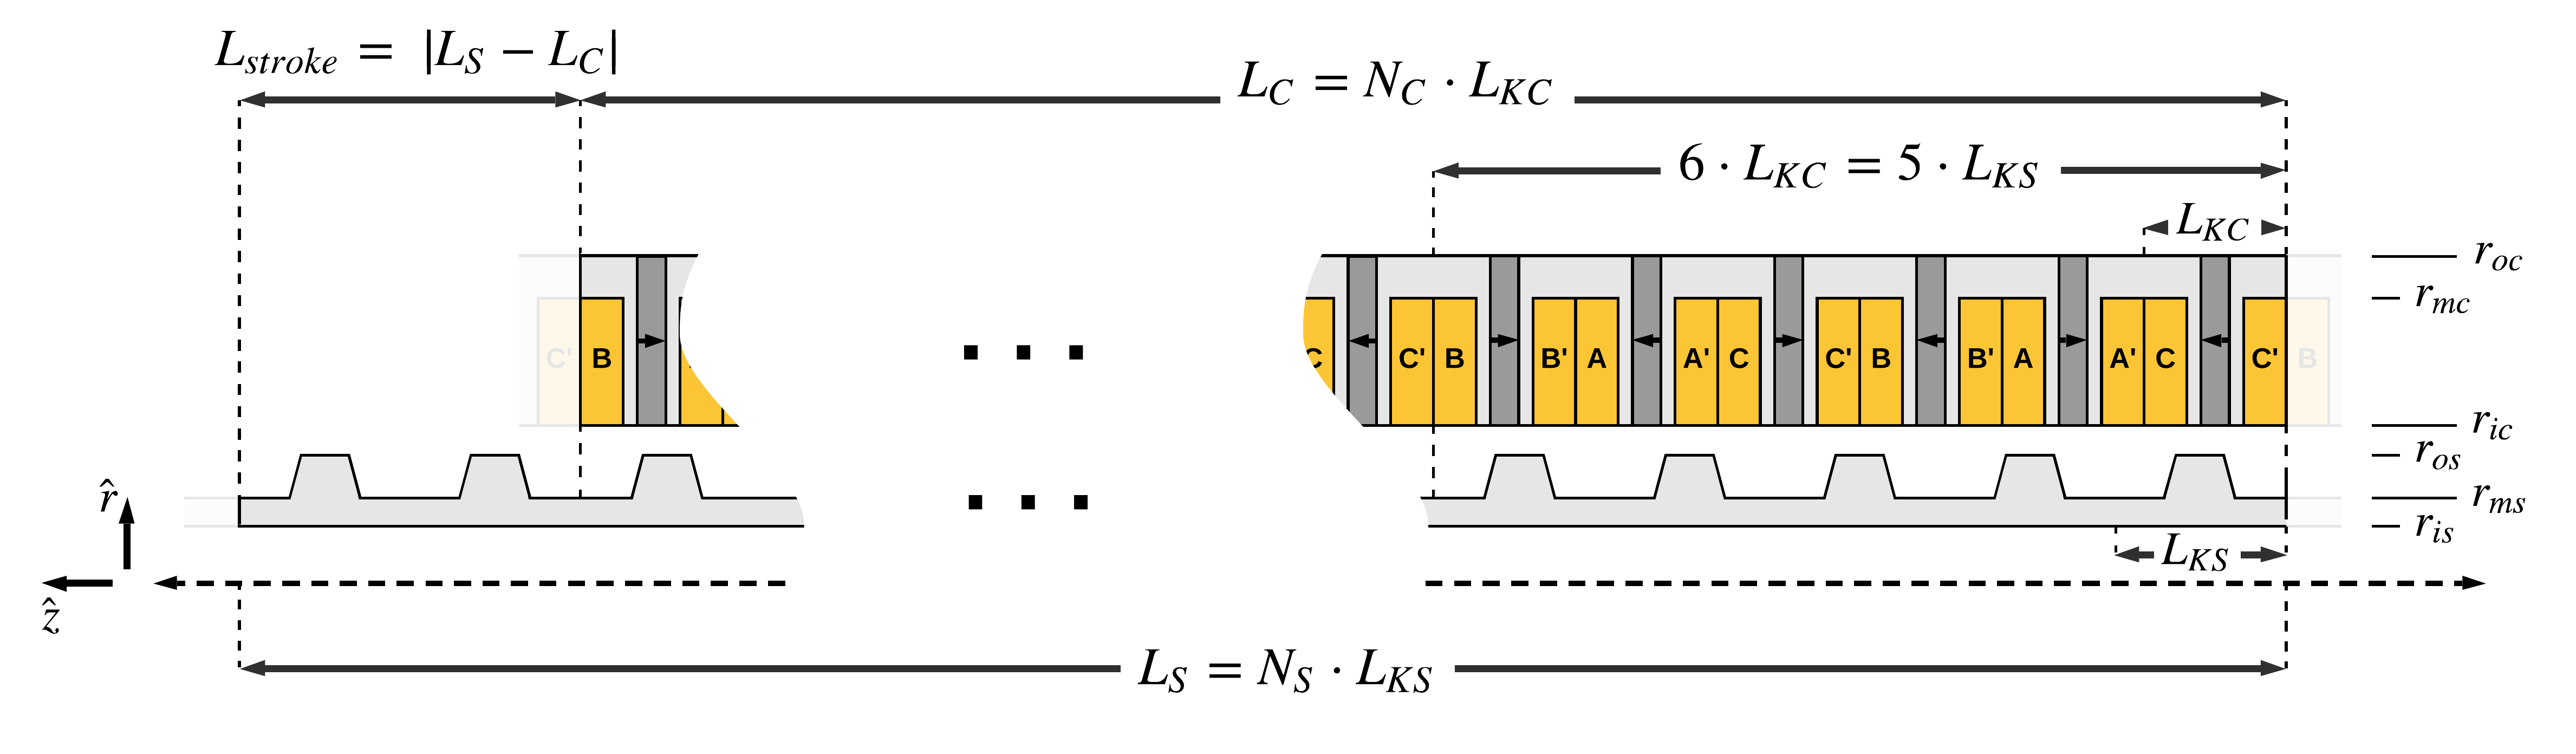
\includegraphics[width=0.97\textwidth]{chap4/images2/LFSM_6_5.png}
            }
            \caption{Schematic of tubular \acs{LFSM}
                \label{fig:conventional_flux_switching_machines}
            }\label{fig:chapter/rsm/LFSM/structure}
        \end{figure*}
        
        
        The general parameters of a three-phase tubular linear flux-switching motor consist of:
        
        \begin{itemize}
            \item The total number of armature slots $N_C$, as opposed to the number of half-coil phases $N_M$ in \acsp{PMLSM},
            \item The total number of armature pole $N_S$, which is different from the number of half-magnet phases in \acsp{PMLSM},
            \item The radii of the \acs{SMC} track $r_{is}$, $r_{ms}$, and $r_{os}$,
            \item The radii of the armature assembly $r_{ic}$, $r_{mc}$, and $r_{oc}$,
            \item The slot period length $L_{KC}$,
            \item The track period length $L_{KS}$,
            \item The whole of mover armature length $L_{C}$,
            \item The whole track length or equivalent motor length $L_{S}$, which does not represent the stroke length like in \acsp{PMLSM},
            \item The length of each overall repeat unit $L_{repeat}$ of $6$ coil slots and $7$ track poles,
            \item The motor stroke length $L_{stroke}$.
        \end{itemize}
        
        
        \begin{figure*}
            \centering
            \subfloat[\label{fig:chapter/rsm/LFSM/machine design/params} Detailed dimensions]{
                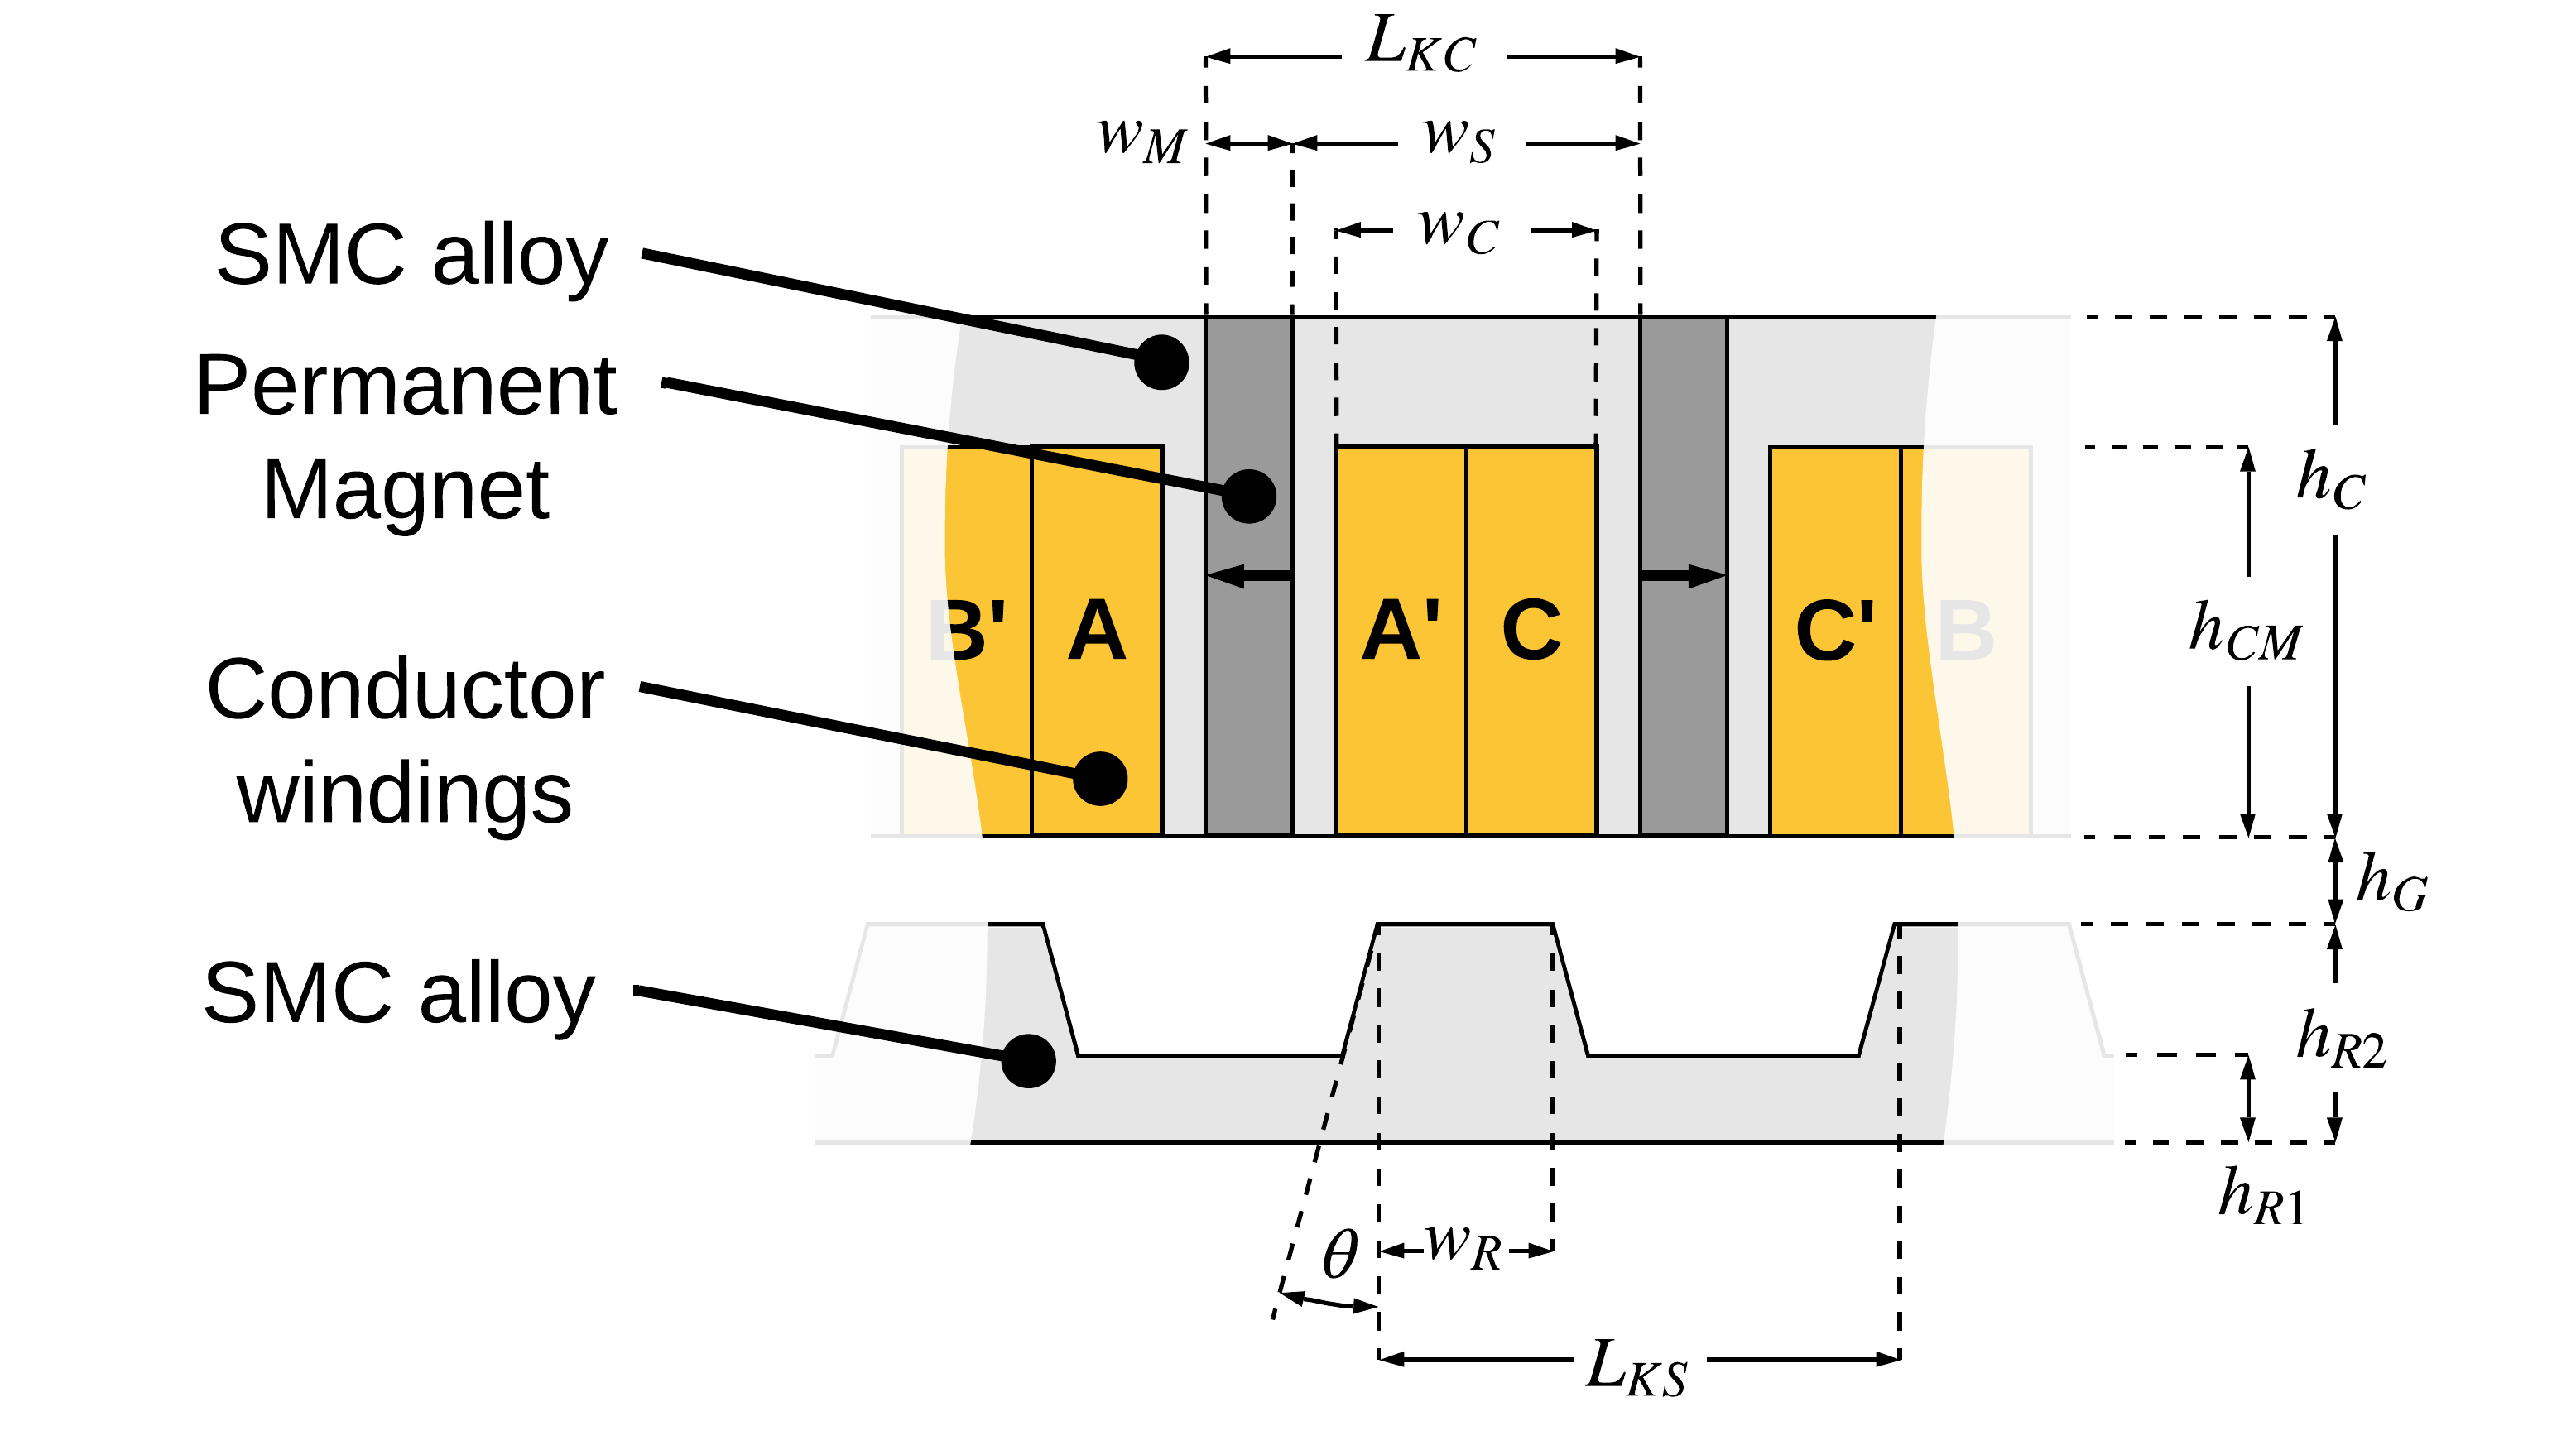
\includegraphics[width=0.7\textwidth]{chap4/images2/params.png}
            }
            \\
            \subfloat[\label{fig:chapter/rsm/LFSM/machine design/setup} A jet injector driven by a LFSM]{
                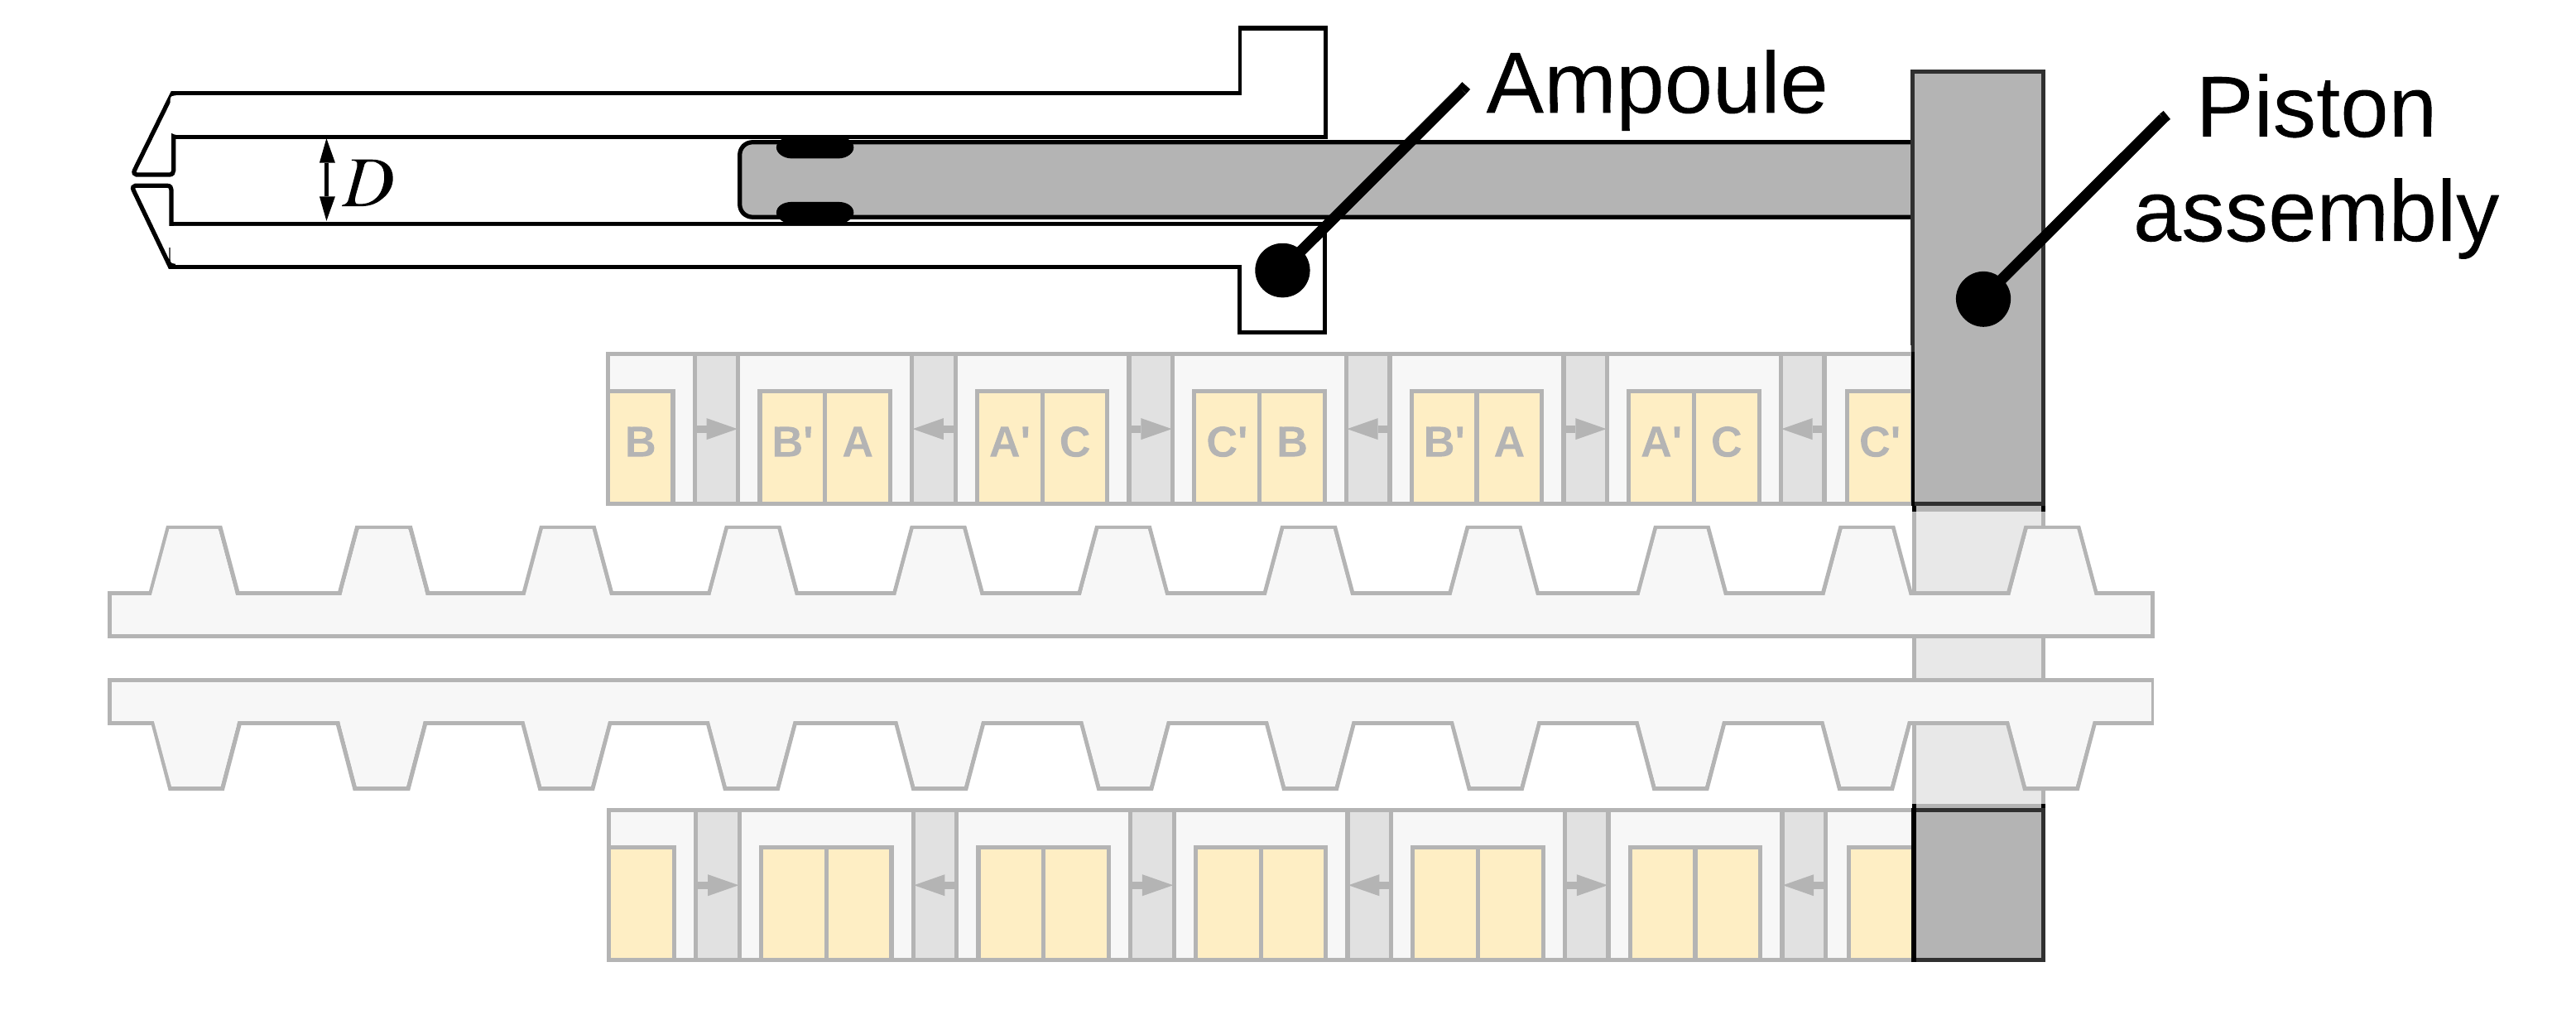
\includegraphics[width=0.8\textwidth]{chap4/images2/machine_setup.png}
            }
            \caption{ 
                \label{fig:chapter/rsm/LFSM/machine design}Detailed dimensions of the tubular LFSM: 
                armature assembly widths ($w_M$, $w_S$, $w_C$),
                armature assembly heights ($h_{CM}$, $h_{C}$),
                track tooth width ($w_{R}$),
                and track tooth heights ($h_{R1}$, $h_{R2}$), tooth angle $\theta$, air gap $h_G$ in $\mathrm{(a)}$. A basic schematic of a LFSM driven jet injector and a NFJI drug ampoule with diameter $D$ are shown in $\mathrm{(b)}$.
            }
        \end{figure*}
        
        
        To minimize the moving (and total) mass, the outer sliding armature assembly was selected as the moving element. Each repeating period of the mover consists of six axially magnetized permanent magnet rings, six \acf{SMC} cylindrical cores to contain the conductor windings, and two circumstantially wound three-phase coil groups. The secondary is passive, and constructed as an SMC tube with a periodic tooth structure with angled sides. Dimensions are shown for each topology in Fig.\,\ref{fig:chapter/rsm/LFSM/machine design/params}. Additionally, Fig.\,\ref{fig:chapter/rsm/LFSM/machine design/setup} illustrates how a tubular \acs{LFSM} can be incorporated in the design of a hand-held jet injector device. Different lengths of the topology are governed by the following equations:
        
        
        \begin{equation}
            L_{repeat}=6\,L_{KC}=7\,L_{KS}
            \label{eq:chap/rsm/LFSM/L_repeat,LKC,LKS}
        \end{equation}
        
        \begin{equation}
            L_{C}=N_C\,L_{KC}
            \label{eq:chap/rsm/LFSM/L_C}
        \end{equation}
        
        \begin{equation}
            L_{S}=N_S\,L_{KS}
            \label{eq:chap/rsm/LFSM/L_S}
        \end{equation}
        
        
        \begin{equation}
            L_{stroke}= \big| L_S-L_C \big|
            \label{eq:chap/rsm/LFSM/L_stroke}
        \end{equation}
        
        
        Additional design ratios were established to better capture the parametric representation of the 6 slot/7 pole tubular \acs{LFSM}:
        
        
        \begin{equation}
            \alpha=\frac{w_M}{L_{KC}}
            \label{eq:chap/rsm/LFSM/alpha}
        \end{equation}
        
        
        \begin{equation}
            \beta=\frac{w_C}{w_S}
            \label{eq:chap/rsm/LFSM/beta}
        \end{equation}
        
        
        \begin{equation}
            \gamma=\frac{h_{CM}}{h_C}
            \label{eq:chap/rsm/LFSM/gamma}
        \end{equation}
        
        
        \begin{equation}
            \delta=\frac{w_R}{L_{KS}}
            \label{eq:chap/rsm/LFSM/delta}
        \end{equation}
        
        
        \begin{equation}
            \epsilon=\frac{h_{R1}}{h_{R2}}
            \label{eq:chap/rsm/LFSM/epsilon}
        \end{equation}

    
        In later subsections, the aim of the work is to examine the performance of \acs{LFSM} for \acs{NFJI} tasks using a process described in Section\,\ref{Chapter:RSM/outline} and demonstrated in Section\,\ref{Chapter:RSM/PMLSM}. Fig.\,\ref{fig:chapter/rsm/LFSM/design process} illustrates the \acs{RSM} design process adapted to the \acs{LFSM} topology above. 
    
    
        \begin{figure*}
            \centering
            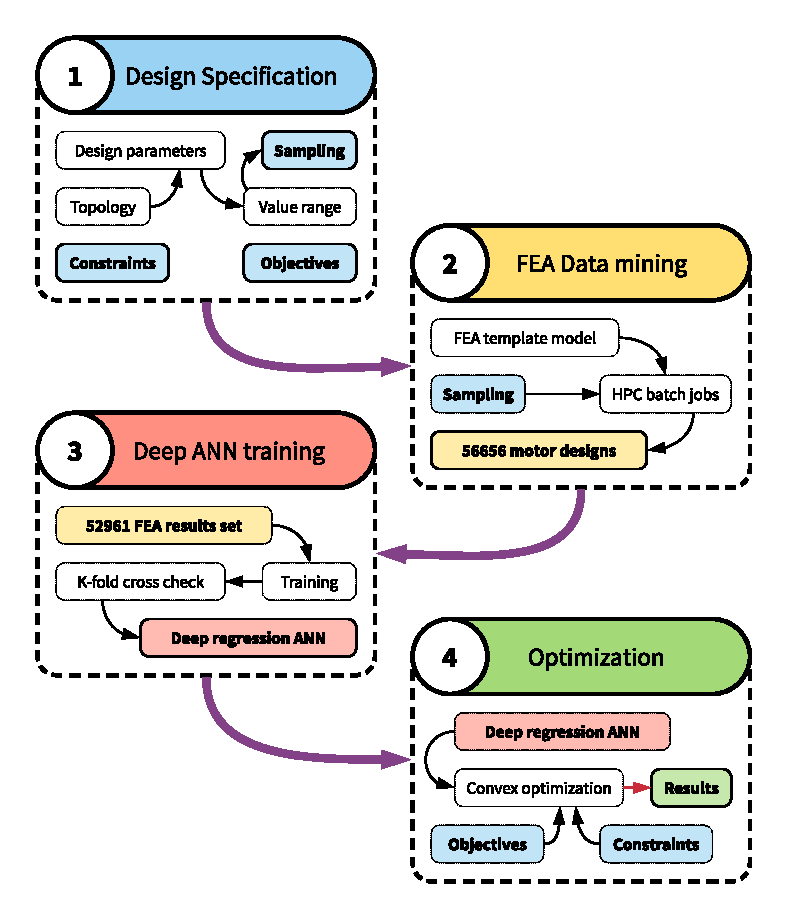
\includegraphics[width=4.5in]{chap4/images2/LFSM_design_process.pdf}
            \caption{Flowchart of the RSM motor design process adapted for \acs{LFSM}.}
            \label{fig:chapter/rsm/LFSM/design process}
        \end{figure*}
    
    
        % -----------------------------------------------------------------------------------
        % --- NEW SUB SECTION --- NEW SUB SECTION --- NEW SUB SECTION --- NEW SUB SECTION --- 
        % -----------------------------------------------------------------------------------
        \subsection{Specifications \& Samplings}    \label{Chapter:RSM/LFSM/spec}
        
        
            This work investigated and optimized a tubular linear 6 slot/7 pole machine with the dimensions presented in Fig.\,\ref{fig:chapter/rsm/LFSM/structure} and \,\ref{fig:chapter/rsm/LFSM/machine design}. With consideration to the dimensions and ratios of the desired motor design, the structural design factors and their range are summarized in Table\,\ref{table:chap/rsm/LFSM/design range}. 
            
            
            The magnet, conductor and \acs{SMC} core assembly as a whole body was treated as the mover, and the \acs{SMC} track with trapezoid teeth was treated as the stator. Similar to the tubular \acs{PMLSM}, the stator core inner radius $r_{si}$ and the mover-stator air gap $h_G$ are fixed at $2\mathrm{mm}$ and $1.2\mathrm{mm}$, respectively. With an effective stator pocket of $4\,\mathrm{mm}$ in diameter, the structural support has a space to be added later on. For the ease of manufacturing, there required a reasonable amount of air gap between the stator and mover such as $1.2\mathrm{mm}$, which comes from our past experience building tubular longitudinal synchronous motor. Physically, this air gap will include non-magnetic support structures as well as mechanical clearance. Note that in the data collection process, the motor length $L_S$ and stroke length $L_{stroke}$ were yet to be determined. Instead, the length of each repeat 6 slot/7 pole unit $L_{repeat}$ was iterated upon. To simplify the model, the tooth angle $\theta$ was set to be a fixed value of $\arctan{1/2}$, which makes the width of each tooth extension precisely half the height of the teeth.
            
            
            Table\,\ref{table:chap/rsm/LFSM/sampling levels} shows incremental sampling steps for the structural design factors. From the sampling steps, a design grid of $46656$ cases was generated. Additionally, another $10000$ cases constructed by input variables created with random values within Table\,\ref{table:chap/rsm/LFSM/design range} range were added to help generalize the entire continuous design space better. In total, there were $56656$ independent motor designs to have their average thrust, maximum thrust, and cogging profile predicted by \acs{FEA}.
            
            
            \begin{table}
                \renewcommand{\arraystretch}{1.2}
                \caption{Summary of the \acs{LFSM} motor parameter ranges}
                \label{table:chap/rsm/LFSM/design range}
                \centering
                \begin{tabular}{@{}llr@{}}
                \hline
                \bfseries Parameter & \bfseries Description & \bfseries Values\\
                \hline
                    $\alpha$	    & Ratio of $w_M$ over $L_{KC}$              &	$0.1-0.4$\\ 
                    $\beta$	        & Ratio of $w_C$ over $w_S$		            &	$0.4-0.9$\\ 
                    $\gamma$	    & Ratio of $h_{CM}$ over $h_C$			    &	$0.6-0.9$\\ 
                    $\delta$	    & Ratio of $w_R$ or $L_{KS}$		        &	$0.1-0.3$\\ 
                    $\epsilon$	    & Ratio of $h_{R1}$ or $h_{R2}$		        &	$0.4-0.6$\\ 
                    $r_{si}$	    & Inner radius of SMC stator core 	        &	$2\,\mathrm{mm}$\\ 
                    $r_{so}$	    & Outer radius of SMC stator core 			&	$4-10\,\mathrm{mm}$\\ 
                    $h_C$           & Thickness of the mover assembly           &	$5-30\,\mathrm{mm}$\\ 
                    $h_G$	        & Mover-stator air gap 					    &	$1.2\,\mathrm{mm}$\\ 
                    $L_{repeat}$	& Length of each 6 slot/7 pole unit 		&	$50-90\,\mathrm{mm}$\\ 
                    $\theta$	    & Stator tooth angle 		                &	$\arctan(1/2)$\\ 
                    $N_C$	        & Number of armature slots 		            &	$6$\\ 
                    $N_S$	        & Number of mover pole 		                &	$7$\\ 
                \hline
                \end{tabular}
            \end{table}
            
            
            \begin{table}
                \renewcommand{\arraystretch}{1.2}
                \caption{Summary of the \acs{LFSM} motor parameter sampling levels}
                \label{table:chap/rsm/LFSM/sampling levels}
                \centering
                \begin{tabular}{@{}l r r r r r r r@{}}
                \hline
                \bfseries Params & \bfseries Level 1 & \bfseries Level 2 & \bfseries Level 3 & \bfseries Level 4 & \bfseries Level 5 & \bfseries Level 6 & \bfseries Unit \\
                \hline
                    $\alpha$     & 0.1     & 0.2  & 0.3 & 0.4 & -   & -   &               \\
                    $\beta$      & 0.4     & 0.5  & 0.6 & 0.7 & 0.8 & 0.9 &               \\
                    $\gamma$     & 0.6     & 0.7  & 0.8 & 0.9 & -   & -   &               \\
                    $\delta$     & 0.1     & 0.2  & 0.3 & -   & -   & -   &               \\
                    $\epsilon$   & 0.4     & 0.5  & 0.6 & -   & -   & -   &               \\
                    $r_{so}$     & 4       & 7    & 10  & -   & -   & -   &               \\
                    $h_C$        & 5       & 10   & 15  & 20  & 25  & 30  & $\mathrm{mm}$ \\
                    $L_{repeat}$ & 50      & 70   & 10  & -   & -   & -   & $\mathrm{mm}$
                    \\
                \hline
                \end{tabular}
            \end{table}
                    
        
        % -----------------------------------------------------------------------------------
        % --- NEW SUB SECTION --- NEW SUB SECTION --- NEW SUB SECTION --- NEW SUB SECTION --- 
        % -----------------------------------------------------------------------------------
        \subsection{\acs{FEA} data mining}          \label{Chapter:RSM/LFSM/data mining}
        
            
            There is an abundance of studies which have explored the effects of changing single design parameters or a few at a time; however, there has not been a study that examines the effect of scaling all \acs{LFSM} design parameters to benchmark a scaling law. The flux loading created by the permanent magnets pushes the iron structures close to saturation in some locations of the motor, thus the form of the scaling law cannot be a linear constant. An arbitrary 6 slot/7 pole machine and a machine with the same structure but all dimensions doubled ("$2\times$ motor") were compared. Fig.\,\ref{fig:chap/rsm/LFSM/periodic_fea/thrust_waveform_study} provides the contrast of the force production capability at different stroke positions for the original motor and the "$2\times$ motor". The periodic \acs{FEA} setup is illustrated in Fig.\,\ref{fig:chap/rsm/LFSM/periodic_fea/fea_for_studies}. Notice that the thrust waveforms are uneven, with high ripple and skewness, which both grow as the current density is increased. Due to the unevenness of the thrust waveform, the average thrust $\overline{F}$ and associated average \acs{NFJI} jet speed $\overline{v_{jet}}$ needs to be estimated by calculating the mean of various thrust measurements at different coil-tooth offsets.
            
            
            \begin{figure*}[!ht]
                \centering
                \subfloat[\label{fig:chap/rsm/LFSM/periodic_fea/fea_for_studies} FEA setup for the thrust waveform plot and current scaling study. The teeth angle $\theta = 0^\circ$.]{
                    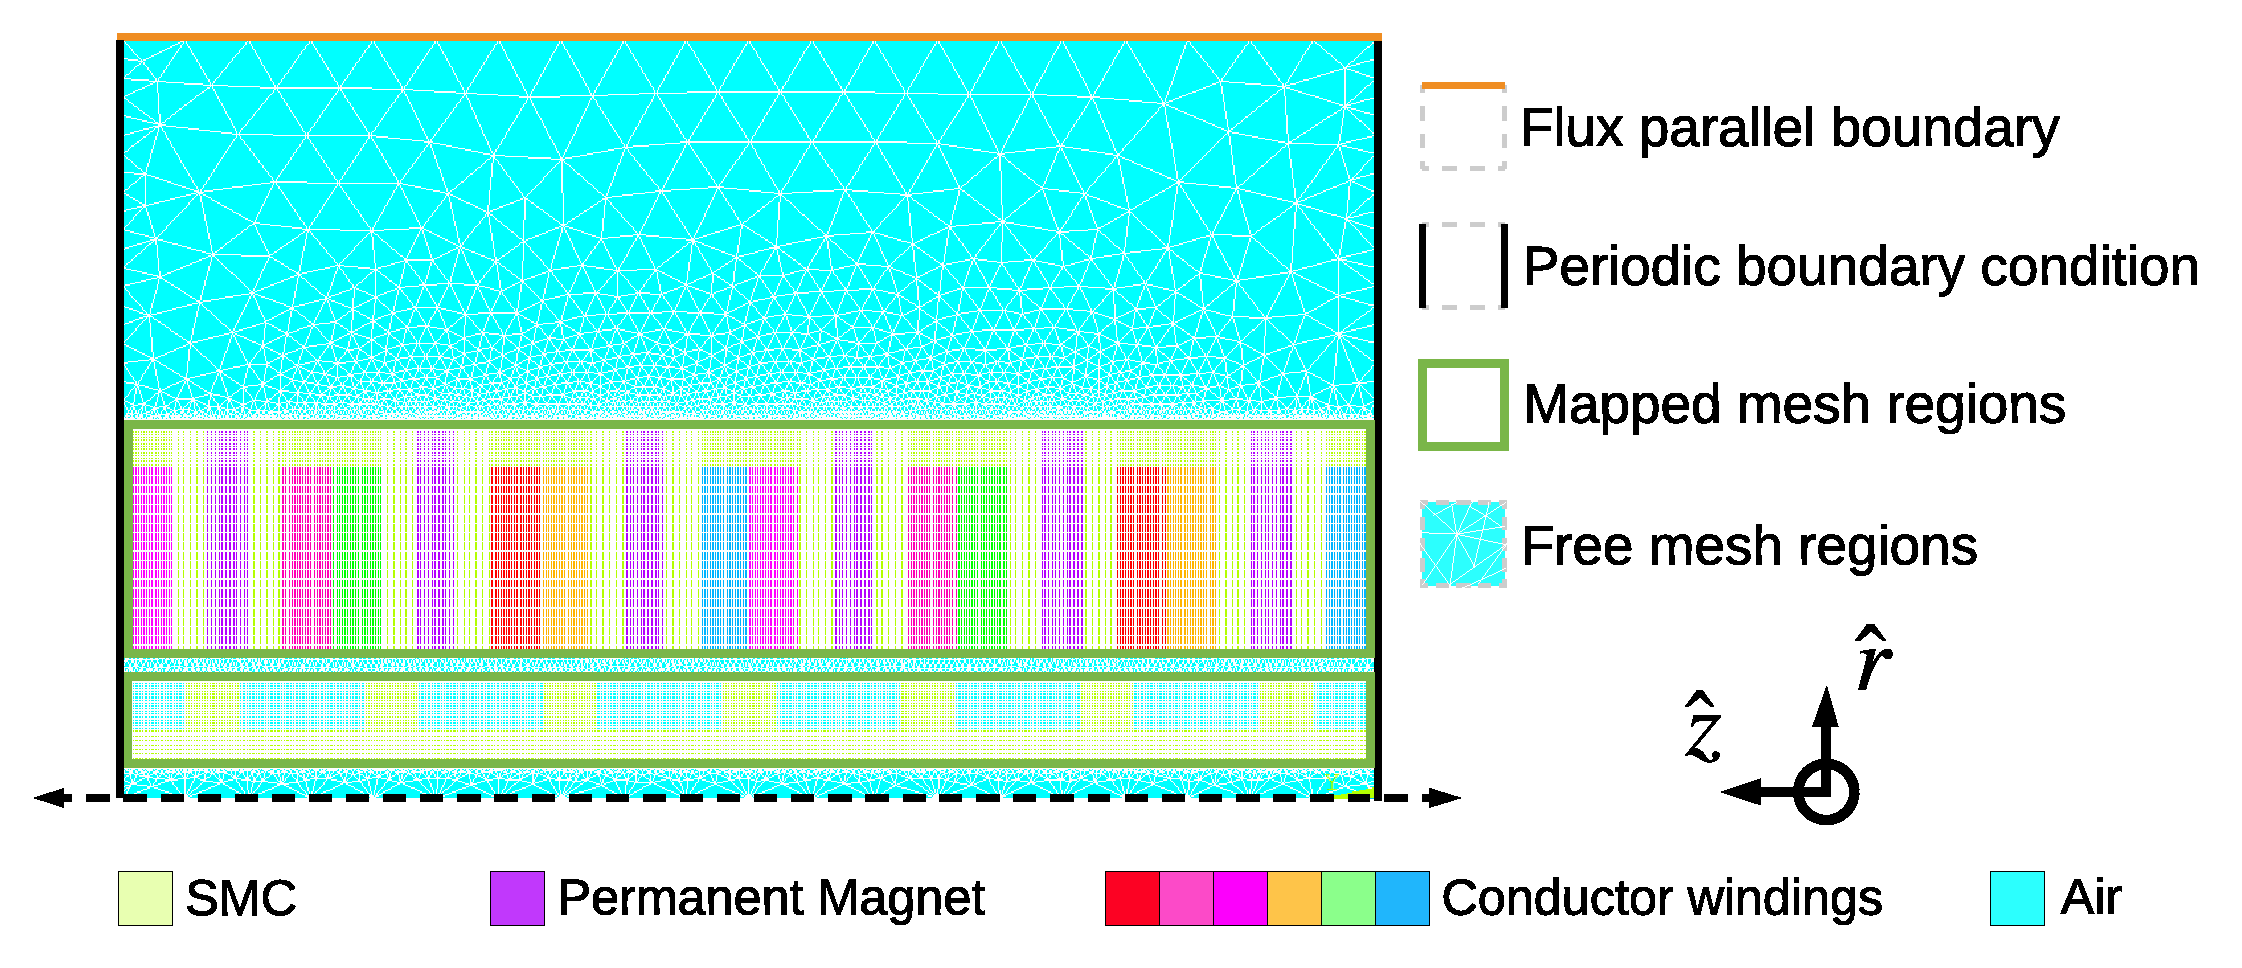
\includegraphics[width=0.98\textwidth]{chap4/images2/LFSM_periodic_setup.pdf}
                }
                \par\bigskip
                \subfloat[\label{fig:chap/rsm/LFSM/periodic_fea/thrust_waveform_study} 
                    1x motor: 
                    6 slots, 
                    7 poles, 
                    $r_{is}=\mathrm{2mm}$, 
                    $h_{R1}=\mathrm{2.4mm}$, 
                    $h_{R2}=\mathrm{6mm}$,
                    $r_{ic}=\mathrm{9.2mm}$,
                    $h_{C1}=\mathrm{12mm}$, 
                    $h_{C2}=\mathrm{15mm}$, 
                    $w_{M}=\mathrm{2.7mm}$,
                    $w_{S}=\mathrm{10.6mm}$,
                    $w_{C}=\mathrm{6.4mm}$,
                    $w_{R}=\mathrm{3.4mm}$,
                    $6\cdot L_{KC}=7\cdot L_{KS}=\mathrm{80mm}$, $\theta = 0^\circ$.
                    ]{
                    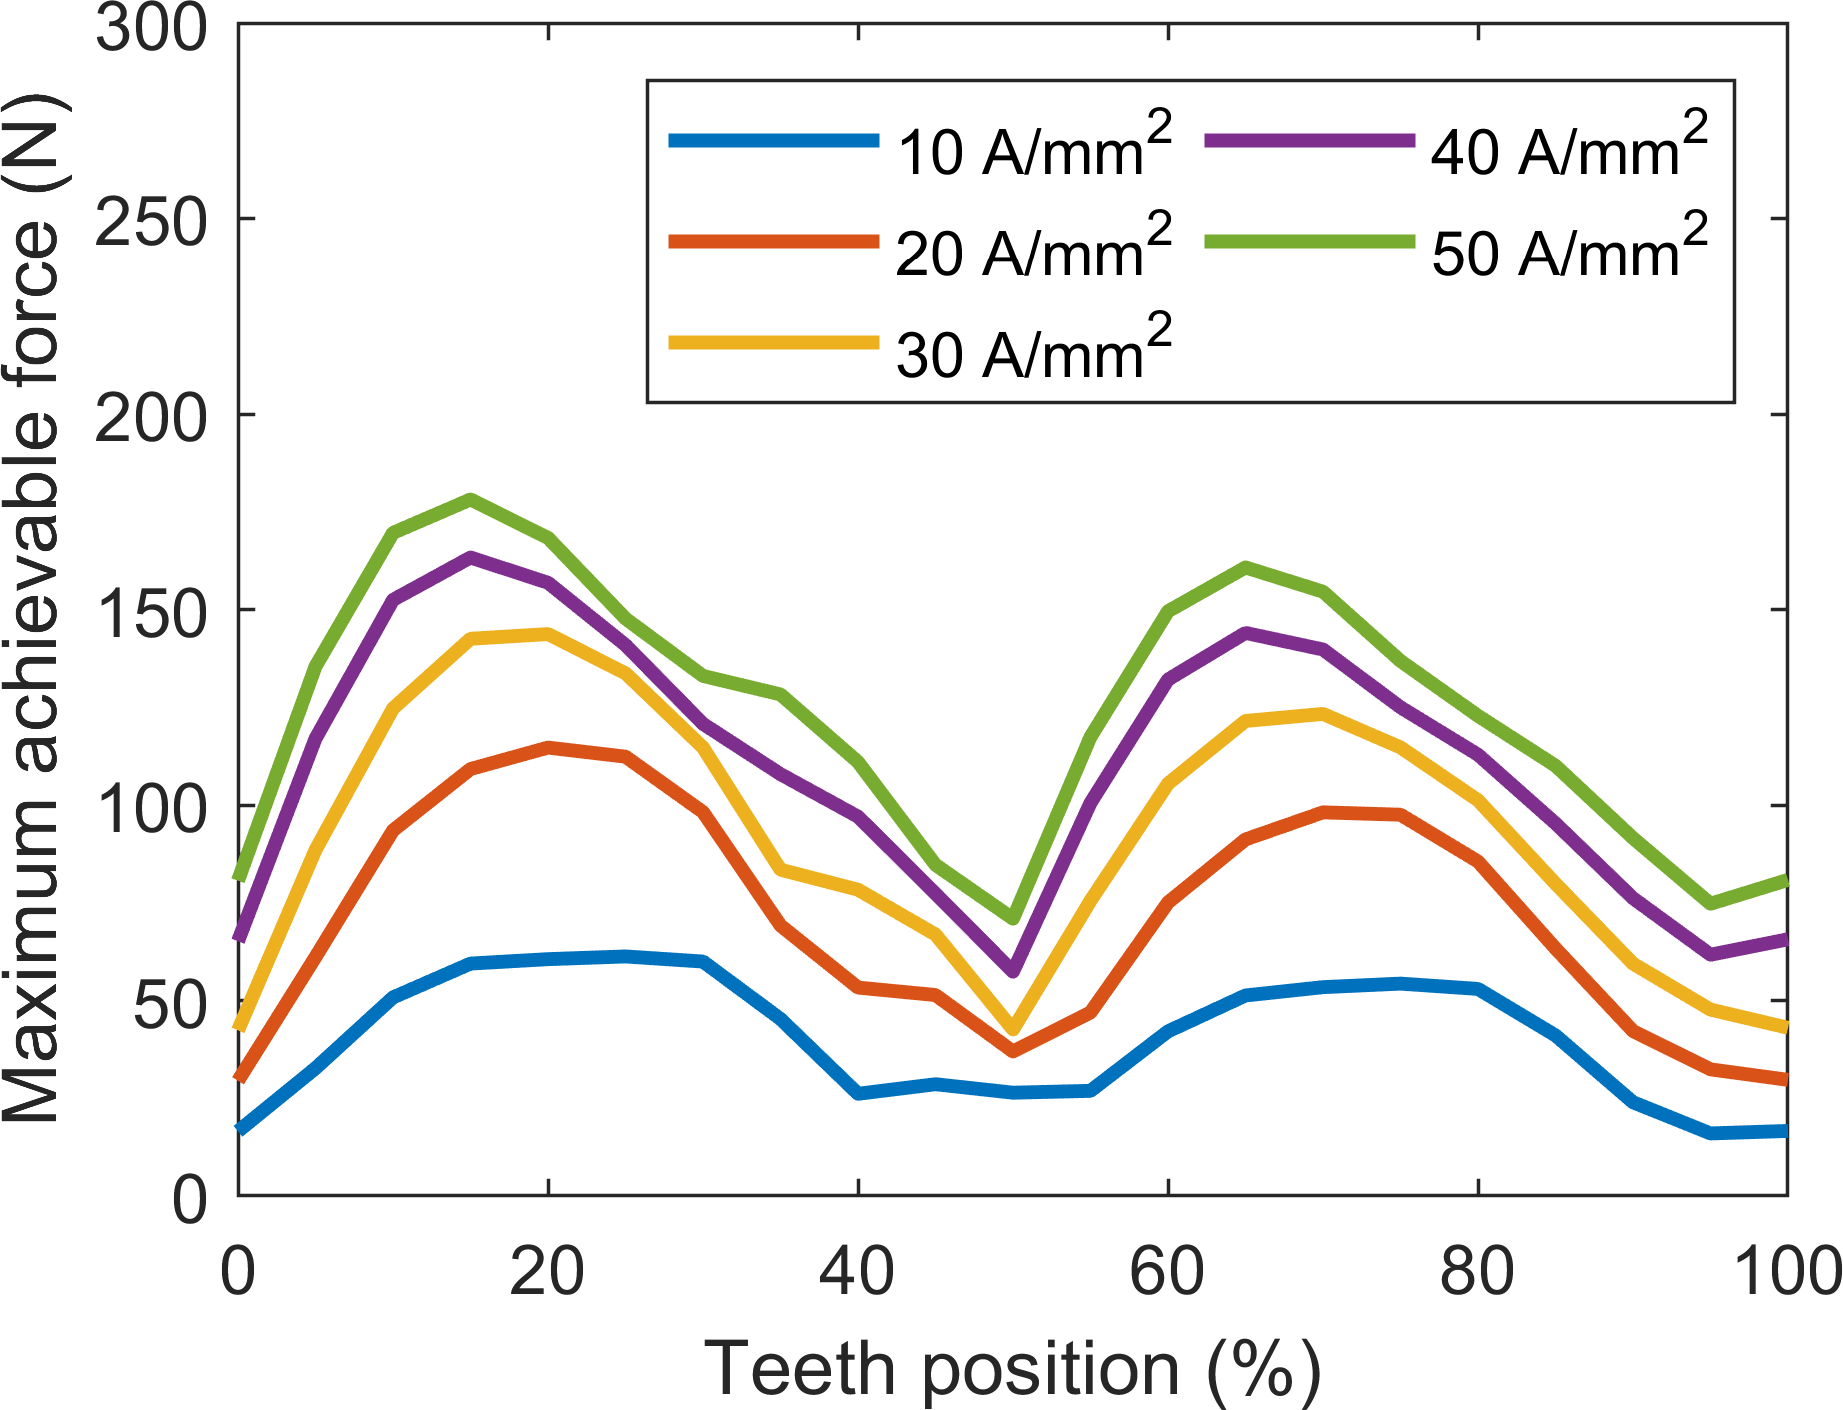
\includegraphics[width=0.45\textwidth]{chap4/images2/LFSM_thrust_waveform.png}
                }
                \,\,\,\,\,\,\,\,
                \subfloat[\label{fig:chap/rsm/LFSM/periodic_fea/scaling_study}
                    Plot of average thrust for the original motor and another motor with all dimensions doubled (``2x motor") at different current densities: $1$, $3$, $5$, $10$, $20$, $30$, $40$, and $50\,\mathrm{A/mm^2}$
                    ]{
                    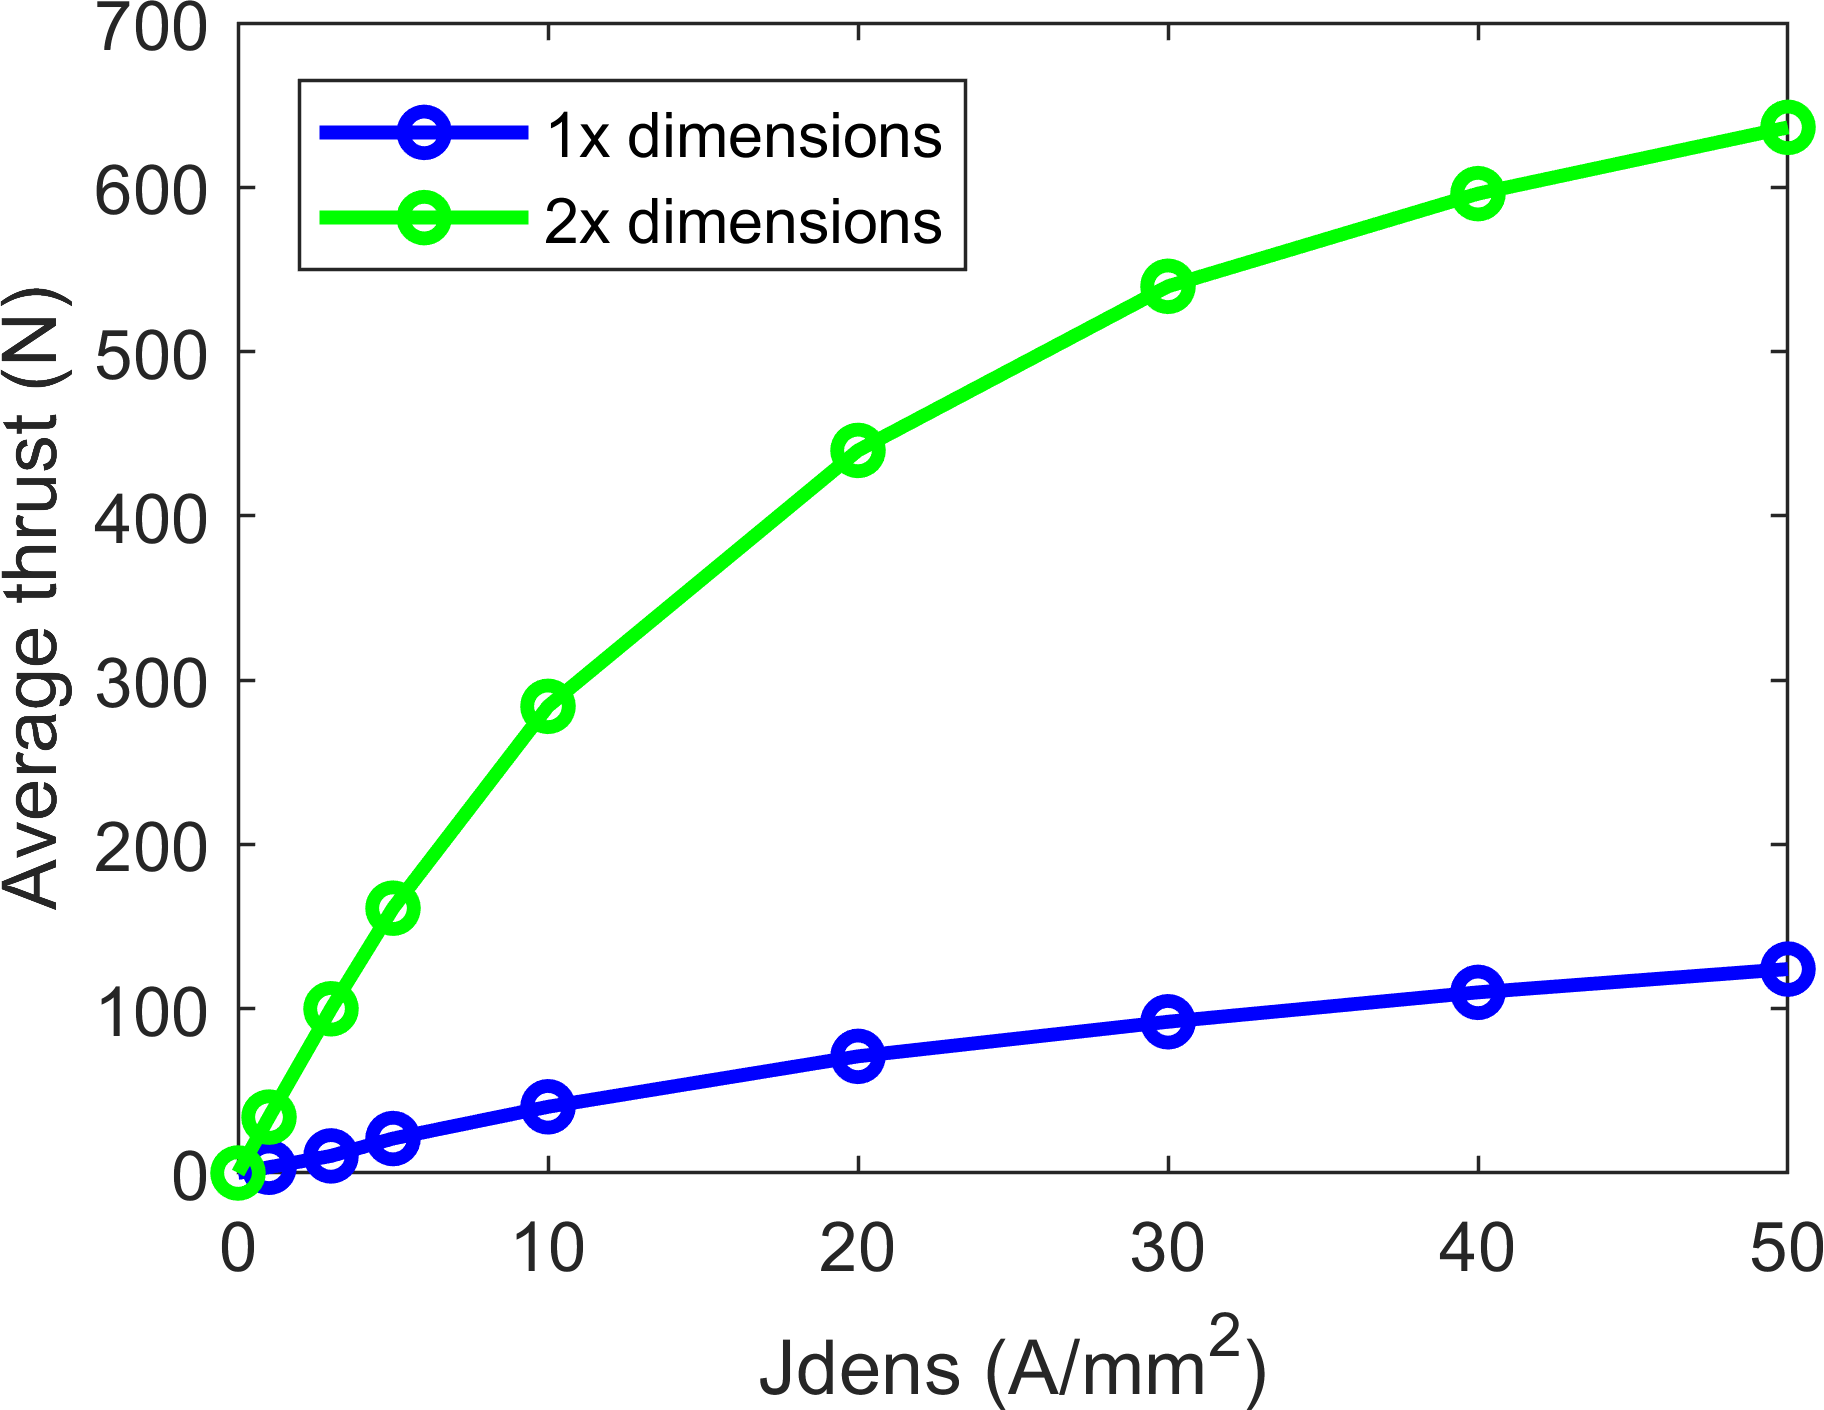
\includegraphics[width=0.45\textwidth]{chap4/images2/LFSM_scaling_effect.png}
                }
                \caption{ 
                    \label{fig:hap/rsm/LFSM/periodic_fea} The axis-symmetric \acs{FEA} model in ANSYS Mechanical APDL for evaluating force produced on the secondary $\mathrm{(a)}$. 
                    A plot of maximum achievable force at different track positions for
                    the original motor moving right $\rightarrow$ left $\mathrm{(b)}$.
                    A plot that compares the original motor's force production capability to that of a motor twice the size $\mathrm{(c)}$.
                }
            \end{figure*}
    
        
            In doubling the dimensions of a motor, the mass and volume are multiplied by a factor of $8$. Hence, when applying the same current density to the coil, the "$2\times$ motor" consumes eight times more power. For a permanent magnet motor, one would expect that the force produced would also be eight times higher, in agreement with the motor constant scaling units of $\mathrm{N/\sqrt{W\cdot kg}}$\,\cite{Ruddy2011DesignMotors}. However, the scaling relationship is different in motors operating primarily on the principle of variable reluctance. The scaling difference arises because, in scaling the overall dimensions of the motor by a fixed number, the rates at which PM and winding induction lose effectiveness are different\,\cite{Melcher1981ContinuumElectromechanics}. In a \acs{LFSM}, the thrust is produced from the flux-switching action of the armature on uni-polar flux produced by the permanent magnet\,\cite{Cheng2011}, a combination of the two operating principles. These scaling relationships apply only up to a certain power level, and above this power level, the motor performance is impacted by saturation.  
    
    
            The effect of scaling this \acs{LFSM} is shown in Fig.\,\ref{fig:chap/rsm/LFSM/periodic_fea/scaling_study}. In this particular example, for a current density up to $5\,\mathrm{A/ mm^2}$, the force produced by the "$2\times$ motor" was indeed eight times that of the original motor. This ratio dropped to seven times at $10\,\mathrm{A/ mm^2}$ and to below six times at $40\,\mathrm{A/ mm^2}$. When optimizing a motor to maximize the motor constant, one should incorporate an extra step to check whether the applied power has not exceeded the scaling relationship implied by the objective of the optimization. The motor constant $K_m$ with unit $\mathrm{N/\sqrt{W\cdot kg}}$ or $\mathrm{N/\sqrt{W}}$ cannot be used to reliably predict thrust given the input power for \acs{LFSM}. To account for the unevenness in the thrust waveform non-linearity of the power-to-thrust ratio, there required \acs{FEA} measurements of thrust at different axial offset, and at the exact power level that the optimization problem requires.
            

            The 6 slot/7 pole machine was modelled in ANSYS MAPDL to measure the force generated on the secondary, as shown in Fig.\,\ref{fig:chapter/rsm/LFSM/FEA}. The 2D axis-symmetric model implemented in ANSYS  $19.2$ used a mapped mesh for the motor parts and a free mesh for the transition regions such as the air gap and the free space surrounding the structure. The periodic boundary conditions were not applied at each end of the armature repeat unit along the $\hat{z}$ direction. This setup therefore did not ignore end effects. If the ANSYS MAPDL scripts were to apply the periodic boundary condition at each end of the armature, and at the same time experimented with a non-zero secondary tooth angle, the ANSYS MAPDL model was tested to produce significantly more execution errors. Instead the simulation setup added three extra teeth on each end of the secondary. As the result, all simulation test cases has exactly six armature slots, and 13 teeth. Fig.\,\ref{fig:chapter/rsm/LFSM/FEA/non_periodic_FEA_setup} illustrates the new \acs{FEA} setup for the data mining step. This setup of \acs{LFSM} was chosen over the \acs{FEA} setup in Fig.\,\ref{fig:chap/rsm/LFSM/periodic_fea/fea_for_studies} because it was more robust for non-zero teeth angle $\theta$.
            

            The \acs{SMC} parts and magnets are made out of Sintex \acs{SMC} prototype materials and K$\&$J Magnetics Grade N45SH, respectively. The non-linear $\mathrm{B-H}$ relationship of the \acs{SMC} material was also fully captured in the FEA model. This setup was crucial to the design optimization process, where many different design configurations needed to be tested.
            
            
            \begin{figure*}[!ht]
                \centering
                \subfloat[\label{fig:chapter/rsm/LFSM/FEA/non_periodic_FEA_setup} A \acs{FEA} setup for mining data that is robust against non-zero teeth angle $\theta$.]{
                    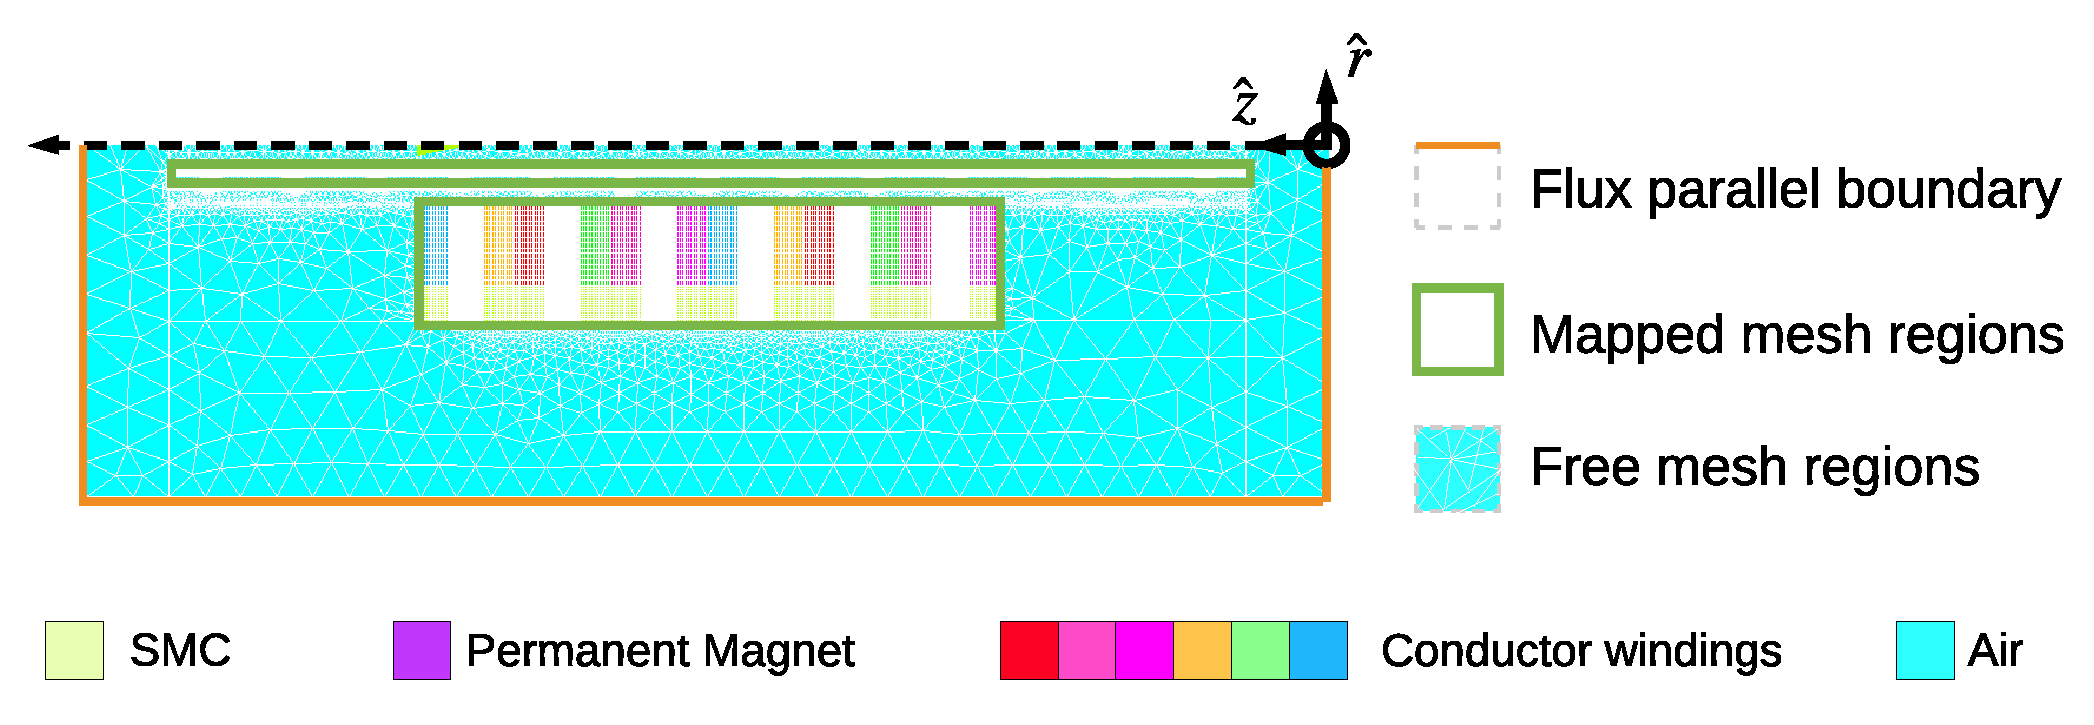
\includegraphics[width=0.98\textwidth]{chap4/images2/FEA_LFSM_non_zero_teeth.pdf}
                }
                \\
                \subfloat[\label{fig:chapter/rsm/LFSM/FEA/position 1} A \acs{FEA} mesh view of \acs{LFSM} for the beginning position]{
                    \includegraphics[width=0.45\textwidth]{chap4/images2/FEA_position_1.png}
                }
                \,\,\,\,\,\,\,\,
                \subfloat[\label{fig:chapter/rsm/LFSM/FEA/position 10} A \acs{FEA} mesh view of \acs{LFSM} for the middle position]{
                    \includegraphics[width=0.45\textwidth]{chap4/images2/FEA_position_10.png}
                }
                \caption{ 
                    \label{fig:chapter/rsm/LFSM/FEA} The FEA setup for obtaining the resultant thrust given a stroke position, a 3-phase current angle, a set of design parameters, and the fixed input power. The graphics cropped from ANSYS MAPDL $19.2$ shows the \acs{SMC} material in green, the free space in blue, the axial permanent magnet rings in dark purple, and the coil phases in orange and light pink.
                }
            \end{figure*}
            
            
            The base modelling script was constructed with the intention to allow for easy modification of the input parameters summarized in Table\,\ref{table:chap/rsm/LFSM/design range}. For the $56656$ motor designs, the unknowns are the cogging force, average thrust, and peak thrust at $1500\,\mathrm{W}$ input power. There were force measurements at $20$ equally spaced stroke positions and $42$ current angle offsets. Since the mesh of each simulation could be re-used for all the different current angle offsets, only the different stroke positions required re-meshing. In total, there were $1133120$ input files which represented all the unique permutations of all motor design dimensions, stroke positions, and current angle offsets. Additionally, each one of the input files contained an extra simulation at null applied current to learn about the cogging force at these various stroke positions. 
            
            
            The $1133120$ input files were sent to the \acf{HPC} infrastructure owned by the New Zealand eScience Infastructure (NeSI) for execution in parallel batches. On average, each one of the input files took $22$ minutes on a two-core Intel CPU with $3\,\mathrm{GBs}$ of RAM. The \acs{HPC} facility allowed for any user to execute $1000$ jobs in parallel. This large simulation job consumed $415506$ CPU hours and took approximately $416$ hours to complete. All verbose output of jobs was collected and doubled checked for errors and warnings, totalling $435\,\mathrm{GBs}$ of raw data in text format. The necessary information was then reduced back to $52961$ fully captured motor designs in CSV format, demonstrating a high success rate of more than $93.5\,\%$. The computed thrust output by \acs{FEA} batches was later further processed and refined into peak to peak cogging force $F_{\Delta cogging}$, average thrust $\overline{F}$, and peak thrust $F_{peak}$ for use in training the neural network.
            
            
            One additional advantage of having the data ready ahead of the optimization process is that the available data, though limited, was able provide valuable insights into identifying the principal design parameters. To investigate these hidden relationships, a co-variance heat map is plotted in Fig.\,\ref{fig:chap/rsm/LFSM/data mining/heat map}. There was a number of useful relationships identified from this heat map:
            
            
            \begin{itemize}
                \item $\alpha$ ratio can improve the average and peak thrust at the cost of more peak to peak cogging $F_{\Delta cogging}$,
                \item $r_{so}$ also improves average and peak thrust without adding more cogging, however, this inherently adds more mass,
                \item Low $\beta$ is more preferable,
                \item Surprisingly, the stator tooth design factors such as $\epsilon$ and $\delta$ have very little influence on the motor performance, even on the peak-to-peak cogging $F_{\Delta cogging}$.
            \end{itemize}
            
            
            \begin{figure}
                \centering
                \includegraphics[width=5in, trim=0 0 0 129mm, clip]{chap4/images2/heatmap.pdf}
                \caption{A co-variance heat map which depicts the relationship between different input and output variables of the motor design data set obtained in the \acs{FEA} data mining step for \acsp{LFSM}. Red and blue on this scale mean positive and negative correlations. Small values are hidden.}
                \label{fig:chap/rsm/LFSM/data mining/heat map}
            \end{figure}
        
        
        % -----------------------------------------------------------------------------------
        % --- NEW SUB SECTION --- NEW SUB SECTION --- NEW SUB SECTION --- NEW SUB SECTION --- 
        % -----------------------------------------------------------------------------------
        \subsection{Deep regression ANN training}   \label{Chapter:RSM/LFSM/ANN training}
        
        
            \begin{figure*}
                \centering
                \subfloat[$70\%-30\%$ split model
                ]{
                    \includegraphics[width=0.5\textwidth]{chap4/images2/MAPE_MSE_6_70-30_SPLIT.png}
                    \label{fig:chapter/rsm/LFSM/training result/MAPE_70_30}
                }
                \subfloat[$75\%-25\%$ split model
                ]{
                    \includegraphics[width=0.5\textwidth]{chap4/images2/MAPE_MSE_6_75-25_SPLIT.png}
                    \label{fig:chapter/rsm/LFSM/training result/MAPE_75_25}
                }
                \\
                \subfloat[$80\%-20\%$ split model
                ]{
                    \includegraphics[width=0.5\textwidth]{chap4/images2/MAPE_MSE_6_80-20_SPLIT.png}
                    \label{fig:chapter/rsm/LFSM/training result/MAPE_80_20}
                }
                \caption{
                    Error produced by the deep learning ANN model to represent \acsp{LFSM} vs. iterations for the training data (blue) and validation data (orange). The \acs{MAPE} is plotted for the training process of (a) $70\%-30\%$, (b) $75\%-25\%$, and (c) $80\%-20\%$ models, respectively.
                }   \label{fig:chapter/rsm/LFSM/training result}
            \end{figure*}
        
        
            The data set provided both the continuous input variables (structural design factors), and the continuous output variable (thrust characteristics at a given power), which classify our application as a supervised and regression type of machine learning problem. The \acs{ANN} model was implemented in Keras and Tensorflow machine learning frameworks:

            
            \begin{itemize}
                \item Eight structural parameters were regarded as the Input Layer: $\alpha$, $\beta$, $\gamma$, $\epsilon$, $\delta$, $r_{so}$, $h_G$, and $L_{repeat}$,
                \item Three performance outputs were regarded as the Output Layer: $F_{\Delta cogging}$, $\overline{F}$, and $F_{peak}$,
                \item The $\mathrm{Adam}$ optimizer was used for \acs{ANN} training,
                \item There were six hidden layers of $256-512-512-512-512-512$ of densely connected nodes,
                \item The rectified linear unit (ReLU) activation function was used
for the input and hidden layers,
                \item The linear activation function was used for the output layer,
                \item The error to optimize for was \acs{MSE},
                \item The training and validation split were chosen at random for each of the three models are: $70\%-30\%$, $75\%-25\%$, and $80\%-20\%$,
                \item The final \acs{ANN} model was ensembled from the average of three models above.
            \end{itemize}


            After 500 training iterations, the model was shown to have a \acf{MAPE} of under $2.41\,\%$. Fig.\,\ref{fig:chapter/rsm/LFSM/training result} shows that the training and validation errors were similar, which means the deep regression model was not over-fitted to the training data set.
        
        
        % -----------------------------------------------------------------------------------
        % --- NEW SUB SECTION --- NEW SUB SECTION --- NEW SUB SECTION --- NEW SUB SECTION --- 
        % -----------------------------------------------------------------------------------
        \subsection{Optimization}                   \label{Chapter:RSM/LFSM/Optimization}
        
        
            \subsubsection{Outer Optimization}          \label{Chapter:RSM/LFSM/Optimization/Outer}
            
            
                In order to fairly compare the performance of \acsp{LFSM} to \acsp{PMLSM} in \acs{NFJI} applications, the optimization problem description needs to be simultaneously adaptable to \acsp{LFSM} and equivalent to that described in Equation\,\ref{eq:outer optimization for PMLSMs}. Note that in the previous section where the \acs{ANN} model was constructed, all designs used to construct the model were limited to a 6 slot/7 pole repeat unit. However, in the optimization problem the number of poles or \acs{SMC} teeth will need to be higher than seven in order to facilitate for the moving coil configuration. The Equation\,\ref{eq:outer optimization for LFSMs} added the last constraint to serve the said condition. The number of coil segments in a single coil repeat unit is six. To increase the number of coil phases, the mover needed to add six coil segments at a time. If more coil phases were added into a fixed length coil, the width of the individual coil winding could be found to be too small and impractical for prototyping. Therefore, the number of coil slots $N_C$ was fixed at six. This effectively made the length of coil $L_C$ the same as the repeat length $L_{repeat}$. The overall optimization for \acs{LFSM} consisted of strategic repetition of the inner optimization to maximize the average jet speed $\overline{v_{jet}}$ derived from the predicted average thrust $\overline{F}$:
                
                
                \begin{itemize}
                    \item   Limit the search to motors with a total length $L_S = L_{C} + L_{stroke}$ in between $120\,\mathrm{mm}$ and $160\,\mathrm{mm}$,
                    \item   Divide the maximum allowed motor length $L_{S-max}$ ranges into 41 equally spaced lists: $[120, 121, 122, ..., 160]\,\mathrm{mm}$ 
                    \item   Divide the coil length $L_{C}$ (equivalent to $L_{repeat}$ because $N_C$ is fixed at a value of $6$) ranges into 41 equally spaced lists:  $[50, 51, 52, ..., 90]\,\mathrm{mm}$ 
                    \item   Create a $\mathrm{2D}$ search zone for each combination of maximum motor length $L_{S-max}$ and coil mover length $L_{C}$, totalling $1681$ points,
                    \item   Run $1681$ inner optimization searches with Matlab constrained convex non-linear optimization function $fmincon()$. Details of the inner optimization will be explained below,
                    \item   Plot and identify a motor design that produces the highest average jet speed $\overline{v_{jet}}$ at the given mass constraint $M_0$.
                \end{itemize}
                
                
                \begin{equation}
                    \begin{array}{rll}
                        \textbf{minimize}       & \small{objective\,\,function}     & f(\textbf{x})=\frac{1}{v_{jet}} \\
                        \textbf{subjected to}   & \small{equality\,\,constraint}    & h_1(\textbf{x})=M - M_0= 0\\
                                                &\quad \small{where}                &\quad  M_0\in\left[325,350,375,400,425\right]\,\mathrm{g}\\
                                                &                                   & h_2(\textbf{x})=P - 1500\,\mathrm{W}=0\\
                                                &                                   & h_3(\textbf{x})=L_C - L_{C0} = 0\\
                                                &\quad \small{where}                &\quad  L_{C0}\in\left[50,51,52,...,90\right]\,\mathrm{mm}\\
                                                &                                   & h_4(\textbf{x})=V - 1\,\mathrm{mL} = 0\\
                                                & \small{inequality\,\,constraint}  & g_1(\textbf{x})=L_S-L_{S-max} \leqslant 0\\
                                                &\quad \small{where}                &\quad L_{S-max} \in \left[120,121,122,...,160\right]\,\mathrm{mm} \\
                                                & \small{other\,\,constraints}       & N_C, N_S \in 	\mathbb{N} \\ 
                                                &\quad \small{where}                &\quad N_C = 6\\
                                                &                                   &\quad N_S \geq 8
                                                \\ \\
                    \end{array}
                    \label{eq:outer optimization for LFSMs}
                \end{equation}
                
                
                
                Given each combination of coil length $L_{C}$ and maximum motor length $L_{S-max}$, the maximum number of whole stator \acs{SMC} teeth $N_S$, the corresponding stator length $L_S$ that can be fitted, and the stroke length $L_{stroke}$ can be derived by the following equations:


                \begin{equation}
                    N_S = \bigg\lfloor  \frac{L_{S-max}}{L_C} \cdot 7 \bigg\rfloor
                    \label{eq:max mumber of teeth for LFSM stator}
                \end{equation}
                
                
                \begin{equation}
                    L_S = {\bigg\lfloor  \frac{L_{S-max}}{L_C} \cdot 7 \bigg\rfloor} \frac{L_C}{7}
                    \label{eq:possible stator length LFSM stator}
                \end{equation}
                
                
                \begin{equation}
                    L_{stroke} = {\bigg\lfloor  \frac{L_{S-max}}{L_C} \cdot 7 \bigg\rfloor} \frac{L_C}{7} - L_C
                    \label{eq:possible stroke length LFSM stator}
                \end{equation}
                
                
                Together with the predicted thrust $F$, ampoule volume $V$, and water density $\rho_w$, the jet velocity $v_{jet}$ can be derived directly from Equation\,\ref{eq:power dissipation for PMLSMs}:
            
            
                \begin{equation}
                    v_{jet} = \sqrt[4]{\frac{4 F {L_{stroke}}^2}{\rho_w V^2}}
                    \label{eq:v_jet for FSM}
                \end{equation}
                
                
            \subsubsection{Inner Optimization}          \label{Chapter:RSM/LFSM/Optimization/Inner}
                
                
                \begin{figure*}
                  \centering
                  \includegraphics[width=5.9in]{chap4/images2/RSM_LFSM_optimization.pdf}
                  \caption{Summary of the top-level motor optimization algorithm and inner optimization routine for \acsp{LFSM}. The algorithm uses motor specifications $V$, $P$, $M$ to determine the motor parameters $\textbf{x}=[\alpha,\beta,\gamma,\delta,\epsilon,r_{so},h_C]$, $N_C$, $N_S$, $L_{repeat}$ at which the jet speed $v_{jet}$ can be maximized.}
                  \label{fig:chapter/rsm/fsm/top level optmization}
                \end{figure*}
                
                
                From a bird eye view, the outer optimization loop provided unique combinations of $L_{C0}$, $L_{S-max}$, and $M_0$ to produce a value of $L_C$, as well as sensible values for $N_S$ and $L_{stroke}$ explained in Equations\,\ref{eq:max mumber of teeth for LFSM stator} and \ref{eq:possible stroke length LFSM stator}. At each point in the $L_{C0} \times L_{S-max}$ space, multiple inner optimizations performed a non-linear constraint optimization for the unknown variables vector $\textbf{x}$:
            
            
                \begin{equation}
                    \textbf{x} = \left[ \alpha,\beta,\gamma,\delta,\epsilon,r_{so},h_{C} \right]
                    \label{eq:inner optimization x of FSM}
                \end{equation}
                
                
                The tooth angle $\theta$ was fixed at $\arctan(1/2)$ to simplify the problem. Other constants such as the inner radius of the stator $r_{si}$, and the mover-stator air gap $h_G$ were made equal to \acsp{PMLSM} inner magnet radius $r_{mi}$, and magnet-coil gap $gap_{mc}$, respectively. The constraints on the input parameters strictly followed the parameter ranges established in Table\,\ref{table:chap/rsm/LFSM/design range} with the only difference of having the value of $N_S$ starting from eight and upward to facilitate for a non-zero stroke length $L_{stroke}$. The inner and outer optimization unknown constraints for \acs{LFSM} are summarized in Table\,\ref{table:chap/rsm/LFSM/optimization unknown constraints}.
                
                
                \begin{table}[!ht]
                    \renewcommand{\arraystretch}{1.2}
                    \caption{Summary of the inner and outer optimization constraints for \acs{LFSM}}
                    \label{table:chap/rsm/LFSM/optimization unknown constraints}
                    \centering
                    \begin{tabular}{@{}llr@{}}
                    \hline
                    \bfseries Parameter & \bfseries Description & \bfseries Values\\
                    \hline
                        $\alpha$	    & Ratio of $w_M$ over $L_{KC}$              &	$0.1-0.4$\\ 
                        $\beta$	        & Ratio of $w_C$ over $w_S$		            &	$0.4-0.9$\\ 
                        $\gamma$	    & Ratio of $h_{CM}$ over $h_C$			    &	$0.6-0.9$\\ 
                        $\delta$	    & Ratio of $w_R$ or $L_{KS}$		        &	$0.1-0.3$\\ 
                        $\epsilon$	    & Ratio of $h_{R1}$ or $h_{R2}$		        &	$0.4-0.6$\\ 
                        $r_{so}$	    & Outer radius of SMC stator core 			&	$4-10\,\mathrm{mm}$\\ 
                        $h_C$           & Thickness of the mover assembly           &	$5-30\,\mathrm{mm}$\\ 
                    \hline
                        $N_C$	        & Number of armature slots 		            &	$6$\\ 
                        $N_S$	        & Number of mover pole 		                &	$\geq 8$\\ 
                        $L_{C0}$	    & Length of coil equality constraint		&	$50-90\,\mathrm{mm}$\\ 
                        $L_{S-max}$	    & Length of stator inequality constraint	&	$120-160\,\mathrm{mm}$\\
                    \hline  \\
                    \end{tabular}
                \end{table}    
                
                
                Each inner optimization aimed at finding $\textbf{x}$ given $[N_C, L_{repeat}, L_{S-max}]$. Each first attempted to find the maximum value of $L_{stroke}$ while rounding down the number of stator teeth $N_S$. The routine then worked to define the unknown $\textbf{x}$ in order to maximize the jet speed $v_{jet}$ with the unknown variable ranges summarized in Table\,\ref{table:chap/rsm/LFSM/optimization unknown constraints}. Additionally, the optimization description in Equation\,\ref{eq:inner optimization for PMLSMs} was applicable for the inner optimization of \acs{LFSM}. The mass term $M$ was obtained via the following set of equations:
                
                
                \begin{equation}
                    w_M = \frac{\alpha}{N_C} L_{repeat}
                    \label{eq:rsm/LFSM/w_m}
                \end{equation}
                
                
                \begin{equation}
                    w_C = \beta\bigg(\frac{L_{repeat}}{N_C}-w_M\bigg);
                    \label{eq:rsm/LFSM/w_c}
                \end{equation}
                
                
                \begin{equation}
                    w_{smc-top} = \frac{1-\beta}{2}\bigg(\frac{L_{repeat}}{N_C}-w_M\bigg)
                    \label{eq:rsm/LFSM/w_smc_top}
                \end{equation}
                
                
                \begin{equation}
                    w_{smc-bot} =  \frac{\delta }{N_S}L_{repeat}
                    \label{eq:rsm/LFSM/w_smc_bot}
                \end{equation}
                
                
                \begin{equation}
                    h_{smc} = r_{oc} - r_{mc}
                    \label{eq:rsm/LFSM/h_smc}
                \end{equation}
                
                
                \begin{equation}
                    \begin{array}{c}
                        V_{stator-repeat} = \pi \bigg[  L_{repeat}  \big({r_{ms}}^2-{r_{is}}^2\big)\\
                        + N_S  \big(r_{os}-r_{ms}\big)\,\tan{\theta}\,\big({r_{os}}^2-{r_{ms}}^2\big)\\
                        + N_S\,w_{smc-bot}\big( {r_{so}}^2 - {r_{ms}}^2 \big)\bigg]
                    \end{array}
                    \label{eq:rsm/LFSM/V_stator_repeat}
                \end{equation}
                
                
                \begin{equation}
                    V_{stator} = \frac{N_S}{N_C}V_{stator-repeat}
                    \label{eq:rsm/LFSM/V_stator}
                \end{equation}
                
                
                \begin{equation}
                    V_{conductor} = \pi\,N_C\,w_c\,\big( {r_{mc}}^2-{r_{ic}}^2 \big)
                    \label{eq:rsm/LFSM/V_conductor}
                \end{equation}
                
                
                \begin{equation}
                    V_{magnet} = \pi\,N_C\,w_m\,\big( {r_{oc}}^2-{r_{ic}}^2 \big)
                    \label{eq:rsm/LFSM/V_magnet}
                \end{equation}
                
                
                \begin{equation}
                    V_{smc-mover} = 2\,\pi\,N_C\,w_{smc-top}\,\big( {r_{mc}}^2-{r_{ic}}^2 \big) + \pi \big( L_{repeat}-N_C w_m \big) \big( {r_{oc}}^2-{r_{mc}}^2 \big) 
                    \label{eq:rsm/LFSM/V_smc_mover}
                \end{equation}
                
                
                \begin{equation}
                    M= V_{stator}\,\rho_{smc} + V_{conductor} \big(0.6\,\rho_c + 0.4\,\rho_{ins} \big) + V_{magnet}\,\rho_{m} + V_{smc-mover}\,\rho_{smc}
                    \label{eq:rsm/LFSM/M}
                \end{equation} \\
                
                
                where the copper fill factor was $60\%$, and material densities $\rho_{smc}$, $\rho_c$, $\rho_{ins}$, $\rho_{m}$ were $7500\,\mathrm{kg/m^3}$, $8920\,\mathrm{kg/m^3}$, $1350\,\mathrm{kg/m^3}$, $7600\,\mathrm{kg/m^3}$, respectively. 
                
                
                Similar to the inner optimizations of \acsp{PMLSM} in Section\,\ref{Chapter:PMLSM design HM/design optimization/optimization formulation/inner} and Section\,\ref{Chapter:RSM/PMLSM/Optimization}, the inner optimization here used constrained nonlinear multi-variable optimization based on the interior point algorithm (MATLAB Optimization Toolbox) to minimize the objective function in Equation\,\ref{eq:inner optimization for PMLSMs}. It should be noted that each objective function evaluation required a prediction of $v_{jet}$, which was inferred by the \acs{ANN} model described in Section\,\ref{Chapter:RSM/LFSM/ANN training}. The method at which the \acs{ANN} was inferred is depicted in Fig.\,\ref{fig:chapter/rsm/PMLSM/inference options/web services}. Upon finishing the inner optimizations for each pair $L_{C0} \times L_{S-max}$, the control flow saved the best performing motor configuration and moved on to the next $L_{C0} \times L_{S-max}$. Fig.\,\ref{fig:chapter/rsm/fsm/top level optmization} summarizes and illustrates both the outer and the inner optimization algorithms.
                
                
                
                
                    

        % -----------------------------------------------------------------------------------
        % --- NEW SUB SECTION --- NEW SUB SECTION --- NEW SUB SECTION --- NEW SUB SECTION --- 
        % -----------------------------------------------------------------------------------
        \subsection{Results}                   \label{Chapter:RSM/LFSM/Results}        
                
            With the objective function evaluation using \acs{ANN} models at its core, the global optimization results of \acs{LFSM} were collected and summarized in Table\,\ref{table:chap/rsm/LFSM/result for global optimization of FSM via RSM method}. The table shows the optimization results for different motor mass constraints $M0 = [325, 350, 375, 400, 425]\,\mathrm{g}$.
            
            
            Looking at one specific result for the global optimization of constraints set $P=1500\,\mathrm{W}$, $V=1\,\mathrm{mL}$, $r_{si}=2\,\mathrm{mm}$, $h_G=1.2\,\mathrm{mm}$, $N_C=6$, $M_0=325\,\mathrm{g}$, $\theta = \arctan{1/2}$ on the search space $L_{C0}:50-90\,\mathrm{mm}$, and $L_{S-max}:120-160\,\mathrm{mm}$, the algorithm found an under-hung \acs{LFSM} with $\alpha=0.36$, $\beta=0.44$, $\gamma=0.63$, $\delta=0.20$, $\epsilon=0.50$, $r_{so}=8.11\,\mathrm{mm}$, $h_C=5.37\,\mathrm{mm}$, $N_S=17$, $L_S=167.86\,\mathrm{mm}$, and $L_{stroke}=92.86\,\mathrm{mm}$. The motor is able to theoretically produce an average thrust $\overline{F} = 129.01\,\mathrm{N}$ and an average jet speed $\overline{v_{jet}}=154.79\,\mathrm{m/s}$. The achievable jet speed was reasonably far from $200\,\mathrm{mm}$, which is known as the jet speed required to guarantee a \acs{NFJI} delivery. 
            
            
            If we now adjust the radius of the drug ampoule so that the average jet speed can reach $200\,\mathrm{m/s}$, the maximum drug volume $V$ can be delivery is now $V_{new}=0.60\,\mathrm{mL}$. This conversion was explained in Equations\,\ref{eq:v_jet and V} and \ref{eq:v_jet and V ratio}. For the optimized motor configurations obtained at mass $M$ of $350\,\mathrm{g}$, $375\,\mathrm{g}$, $400\,\mathrm{g}$, $425\,\mathrm{g}$, the corresponding average jet speed $\overline{v_{jet}}$ are $159.16\,\mathrm{m/s}$, $164.00\,\mathrm{m/s}$, $168.38\,\mathrm{m/s}$, $172.27\,\mathrm{m/s}$, respectively. The reduced volume $V_{new}$ for these motors are $0.63\,\mathrm{mL}$, $0.67\,\mathrm{mL}$, $0.71\,\mathrm{mL}$, and $0.74\,\mathrm{mL}$, in the same order. Fig.\,\ref{fig:chapter/rsm/LFSM/optimization search space result for differnt mass} provides global optimization plots of $\overline{v_{jet}}$ for the search space $L_{S-max}:120\,\mathrm{mm}\rightarrow 160\,\mathrm{mm} \times L_{C0}:50\,\mathrm{mm}\rightarrow 90\,\mathrm{mm}$ using $P=1500\,\mathrm{W}$, $V=1\,\mathrm{mL}$, $r_{si}=2\,\mathrm{mm}$, $h_G=1.2\,\mathrm{mm}$, $N_C=6$, $M_0=325\,\mathrm{g}$, $\theta = \arctan{1/2}$ and $M_0=[325,350,375,400,425]\,\mathrm{g}$. 
 
            
            \begin{landscape}
                \begin{table}
                    \renewcommand{\arraystretch}{1.2}
                    \caption{Summary of \acs{LFSM} design optimization values and performance using \acs{RSM} method}
                    \label{table:chap/rsm/LFSM/result for global optimization of FSM via RSM method}
                    \centering
                    \begin{tabular}{lllrrrrr}
                        \hline
                        \textbf{Params}     & \textbf{Description}                            & \textbf{Unit}           & $M_0=\mathbf{325\,g}$ & $\mathbf{350\,g}$ & $\mathbf{375\,g}$ & $\mathbf{400\,g}$ & $\mathbf{425\,g}$ \\
                        \hline
                        $P$                  & Fixed electrical power input              & $\mathrm{kW}$  & 1.50           & 1.50           & 1.50           & 1.50           & 1.50           \\
                        $V$                  & Volume of NFJI drug ampoule               & $\mathrm{mL}$  & 1.00           & 1.00           & 1.00           & 1.00           & 1.00           \\
                        \hline
                        $L_{C0:optim}$       & Inner loop's $L_C$ at global optimum      & $\mathrm{mm}$  & 65.00          & 62.00          & 70.00          & 70.00          & 70.00          \\
                        $L_{S-max:optim}$    & Inner loop's $L_S$ at global optimum      & $\mathrm{mm}$  & 160.00         & 160.00         & 90.00          & 90.00          & 90.00          \\
                        $\alpha$             & Ratio of $w_M$ over $L_{KC}$              &                & 0.36           & 0.33           & 0.34           & 0.33           & 0.33           \\
                        $\beta$              & Ratio of $w_C$ over $w_S$                 &                & 0.44           & 0.46           & 0.47           & 0.48           & 0.46           \\
                        $\gamma$             & Ratio of $h_{CM}$ over $h_C$              &                & 0.63           & 0.65           & 0.65           & 0.64           & 0.64           \\
                        $\delta$             & Ratio of $w_R$ or $L_{KS}$                &                & 0.20           & 0.18           & 0.19           & 0.18           & 0.19           \\
                        $\epsilon$           & Ratio of $h_{R1}$ or $h_{R2}$             &                & 0.50           & 0.50           & 0.49           & 0.50           & 0.49           \\
                        $r_{si}$             & Inner radius of SMC stator core           & $\mathrm{mm}$  & 2.00           & 2.00           & 2.00           & 2.00           & 2.00           \\
                        $r_{so}$             & Outer radius of SMC stator core           & $\mathrm{mm}$  & 8.11           & 8.59           & 8.78           & 9.02           & 9.30           \\
                        $h_C$                & Thickness of the mover assembly           & $\mathrm{mm}$  & 5.37           & 5.59           & 5.41           & 5.62           & 5.75           \\
                        $h_G$                & Mover-stator air gap                      & $\mathrm{mm}$  & 1.20           & 1.20           & 1.20           & 1.20           & 1.20           \\
                        $L_{repeat}$         & Length of each 6 slot/7 pole unit         & $\mathrm{mm}$  & 65.00          & 62.00          & 70.00          & 70.00          & 70.00          \\
                        $\theta$             & Stator tooth angle                        & $\mathrm{^\circ}$   & 26.56           & 26.56         & 26.56          & 26.56          & 26.56  \\
                        \hline
                        $N_C$                & Number of armature slots                  &                & 6              & 6              & 6              & 6              & 6              \\
                        $N_S$                & Number of mover poles/teeth                      &                & 17             & 18             & 16             & 16             & 16             \\
                        $L_C$                & Length of the moving armature             & $\mathrm{mm}$  & 65.00          & 62.00          & 70.00          & 70.00          & 70.00          \\
                        $L_S$                & Total length of all SMC teeth             & $\mathrm{mm}$  & 157.86         & 159.43         & 160.00         & 160.00         & 160.00         \\
                        $L_{stroke}$         & Real stroke length                        & $\mathrm{m/s}$ & 92.86  & 97.43  & 90.00  & 90.00  & 90.00 \\
                        \hline
                        $\overline{v_{jet}}$ & Average jet speed predicted               & $\mathrm{m/s}$ & 154.79         & 159.16         & 164.00         & 168.38         & 172.27         \\
                        $\overline{F}$       & Average thrust predicted by the ANN & $\mathrm{N}$   & 129.01         & 130.00         & 149.43         & 157.51         & 164.87        \\

                        \hline
                    \end{tabular}
                \end{table}
            \end{landscape}
            
            
            \begin{figure*}[!ht]
                \centering
                \subfloat[$M_0=325\,\mathrm{g}$. Global optimum found at $L_{C0}=65\,\mathrm{mm}$, and $L_{S-max}=160\,\mathrm{mm}$.
                ]{
                    \includegraphics[width=0.45\textwidth]{chap4/images2/325g.png}
                    \label{fig:chapter/rsm/LFSM/optimization/325}
                }
                \qquad
                \subfloat[$M_0=350\,\mathrm{g}$. Global optimum found at $L_{C0}=62\,\mathrm{mm}$, and $L_{S-max}=160\,\mathrm{mm}$.
                ]{
                    \includegraphics[width=0.45\textwidth]{chap4/images2/350g.png}
                    \label{fig:chapter/rsm/LFSM/optimization/350}
                }
                \\
                \subfloat[$M_0=375\,\mathrm{g}$. Global optimum found at $L_{C0}=70\,\mathrm{mm}$, and $L_{S-max}=160\,\mathrm{mm}$.
                ]{
                    \includegraphics[width=0.45\textwidth]{chap4/images2/375g.png}
                    \label{fig:chapter/rsm/LFSM/optimization/375}
                }
                \qquad
                \subfloat[$M_0=400\,\mathrm{g}$. Global optimum found at $L_{C0}=70\,\mathrm{mm}$, and $L_{S-max}=160\,\mathrm{mm}$.
                ]{
                    \includegraphics[width=0.45\textwidth]{chap4/images2/400g.png}
                    \label{fig:chapter/rsm/LFSM/optimization/400}
                }
                \\
                \subfloat[$M_0=425\,\mathrm{g}$. Global optimum found at $L_{C0}=70\,\mathrm{mm}$, and $L_{S-max}=160\,\mathrm{mm}$.
                ]{
                    \includegraphics[width=0.45\textwidth]{chap4/images2/425g.png}
                    \label{fig:chapter/rsm/LFSM/optimization/425}
                }
                \\
                \caption{
                    The global optimization plots of $v_{jet}$ for the search space $L_{M0}:120\,\mathrm{mm}\rightarrow 160\,\mathrm{mm} \times L_{C0}:50\,\mathrm{mm}\rightarrow 90\,\mathrm{mm}$ using $P=1500\,\mathrm{W}$, $V=1\,\mathrm{mL}$, $r_{si}=2\,\mathrm{mm}$, $h_G=1.2\,\mathrm{mm}$, $N_C=6$, $M_0=325\,\mathrm{g}$, $\theta = \arctan{1/2}$,  and $M_0$ of: (a) $325\,\mathrm{g}$, (b) $350\,\mathrm{g}$, (c) $375\,\mathrm{g}$, (d) $400\,\mathrm{g}$, and (e) $425\,\mathrm{g}$.
                }   \label{fig:chapter/rsm/LFSM/optimization search space result for differnt mass}
            \end{figure*}
    
    
    % ===================================================================================================
    % === NEW SECTION === NEW SECTION === NEW SECTION === NEW SECTION === NEW SECTION === NEW SECTION ===
    % ===================================================================================================
    \section{Application to \ac{LTFM}}               \label{Chapter:RSM/LTFM}
    
        
        Conventional longitudinal flux motors like \acs{PMLSM} and \acs{LFSM} requires short repeat lengths for high force density applications because the magnetic circuit travels in-plane with the direction of motion. However, with shortening the pole pitch, the conductor component become increasingly more difficult to manufacture. In \acf{LTFM}, however, the electric circuit is decoupled from the magnetic circuit, and thus the motor can stay manufacturable as the pole pitch shortens. This is because the flux path lies perpendicular to the direction of motion. With this fundamental difference, it is expected that \acs{LTFM} might be able to perform better in short stroke, high thrust applications starting from a near stall condition. 
        
        
        \begin{figure}[!ht]
            \centering
            \subfloat[Schematic for a single phase \acs{LTFM}]{
                \includegraphics[width=0.75\textwidth]{chap4/images3/TFM_illustration.pdf}
                \label{fig:chapter/rsm/LTFM/illustration}
            }
            \\
            \subfloat[3-phase arrangement for \acs{LTFM}]{
                \includegraphics[width=0.5\textwidth]{chap4/images3/TFM_3phase.pdf}
                \label{fig:chapter/rsm/LTFM/3 phase arrangement}
            }
            \caption{Outline of \acs{LTFM} topology.}
            \label{fig:chapter/rsm/LTFM/different LTFM arrangement}
        \end{figure}

        
        This section aimed to study \acs{LTFM} using the motor design process for high volume \acs{NFJI} applications already applied for \acs{PMLSM} and \acs{LFSM}. The chosen topology was the U-core \acs{LFSM} machine, with surface mounted permanent magnet blocks on a long iron stator as shown in Fig.\,\ref{fig:chapter/rsm/LTFM/illustration}. Unlike the inherent 3-phase winding structure of \acs{PMLSM} and \acs{LFSM}, the body of a \acs{LTFM} contains a single rectangular prism for a single conductor winding. There are positions on the stroke of a single phase \acs{LTFM} in which the conductor winding cannot produce any axial thrust no matter how much current is applied. Therefore, three identical copies of this structure must be placed in parallel, and $120^\circ$ apart to facilitate a relatively constant thrust profile with 3-phase current as shown in Fig.\,\ref{fig:chapter/rsm/LTFM/3 phase arrangement}. 
        
        
        \begin{figure*}[!ht]
            \centering
            \subfloat[Dimension outline for a single repeat unit of the \acs{LTFM}]{
                \includegraphics[width=0.95\textwidth]{chap4/images3/TFM_dimensions.pdf}
                \label{fig:chapter/rsm/LTFM/dimensions}
            }
            \\
            \subfloat[The arrangement for using \acs{LTFM} for \acs{NFJI} application]{
                \includegraphics[width=0.85\textwidth]{chap4/images3/TFM_for_NFJI.pdf}
                \label{fig:chapter/rsm/LTFM/used for NFJI}
            }
            \caption{Outline of \acs{LTFM} in \acs{NFJI} application.}
            \label{fig:chapter/rsm/LTFM/3-phase and NFJI}
        \end{figure*}
        
        
         The coil and U-core assembly was chosen to be the mover because this assembly is more likely to be lighter than the magnets and flux conductor plate assembly. Each coil repeating unit consisted of a large conductor winding and U-core made out of prototype \acs{SMC} materials. Each stator repeating unit consisted of four pieces of magnet directed the $y$-axis, and a single long back plate made out of \acs{SMC} material to direct the flux path. Fig.\,\ref{fig:chapter/rsm/LTFM/dimensions} and \ref{fig:chapter/rsm/LTFM/illustration} depict the general parameters of a three-phase transverse flux motor:
        
        \begin{itemize}
            \item The total number of armature repeating unit or pole $N_C$,
            \item The total number of stator and magnets repeating unit or pole $N_M$,
            \item Dimensions related the conductor winding $xx_C$, $yy_C$, and $zz_C$,
            \item Dimensions related to the permanent magnet pieces $xx_M$, $yy_M$, and $zz_M$,
            \item Dimensions related to the U-core made out of \acs{SMC} prototype material $xx_U$, $yy_U$, and $zz_U$,
            \item Dimensions related to the the mover assembly's back plate made out of \acs{SMC} prototype material $xx_B$, $yy_B$, and $zz_B$,
            \item The air gap between the mover and stator assemblies  $zz_{gap}$
            \item The whole of the mover armature length $L_{C}$ for a single phase \acs{LTFM},
            \item The whole track length or equivalent motor length $L_{M}$ for a single phase \acs{LTFM},
            \item Length of an overall repeat unit $L_{repeat}$,
            \item The motor stroke length $L_{stroke}$.
        \end{itemize}
        
        
        \begin{figure*}[!ht]
            \centering
            \includegraphics[width=5in]{chap4/images3/TFM_process_summary.pdf}
            \caption{Flowchart of the RSM motor design process adapted for \acs{LTFM}.}
            \label{fig:chapter/rsm/LTFM/design process}
        \end{figure*}
        
        
        The different lengths of the motor are governed by the following set of equations:
        
        
        \begin{equation}
            L_M = N_M L_{repeat}
            \label{eq:chap/rsm/LTFM/L_M}
        \end{equation}
        
        
        \begin{equation}
            L_C = N_C L_{repeat}
            \label{eq:chap/rsm/LTFM/L_C}
        \end{equation}
        
        
        \begin{equation}
            L_{M-3-phase} = \bigg(1+\frac{2}{3} \bigg) N_M L_{repeat} 
            \label{eq:chap/rsm/LTFM/L_M_3phase}
        \end{equation}
        
        
        \begin{equation}
            L_{C-3-phase} = \bigg(1+\frac{2}{3}\bigg) N_C L_{repeat} 
            \label{eq:chap/rsm/LTFM/L_C_3phase}
        \end{equation}
        
        
        \begin{equation}
            L_{stroke} = \big| L_M-L_C \big| = \big| L_{M-3-phase} - L_{C-3-phase} \big|
            \label{eq:chap/rsm/LTFM/L_stroke}
        \end{equation}
        
        
        where $L_{M-3-phase}$ and $L_{C-3-phase}$ are the length of magnet array and armature in a 3-phase \acs{LTFM}.

        
        
        Additional design ratios were established to better capture the parametric representation of the \acs{LTFM}:
        
        
        \begin{equation}
            \alpha=\frac{2\,xx_M}{L_{repeat}}
            \label{eq:chap/rsm/LTFM/alpha}
        \end{equation}
        
        
        \begin{equation}
            \beta=\frac{yy_C}{yy_M}
            \label{eq:chap/rsm/LTFM/beta}
        \end{equation}
        
        
        \begin{equation}
            \gamma=\frac{zz_U}{zz_C}
            \label{eq:chap/rsm/LTFM/gamma}
        \end{equation}
        
        
        For the rigidity of the structure, the coil and the SMC back plate should be made continuous in motors with non-unity pole numbers. For this very reason, the dimensions $xx_B$ and $xx_C$ were assumed to be equal to $L_{repeat}$:
        
        
        \begin{equation}
            xx_B = xx_C = L_{repeat}
            \label{eq:chap/rsm/LTFM/xb is xc is lrepeat}
        \end{equation}
        
        
        To further simply the topology, $xx_M$, and $yy_M$ were set to be equal to $xx_U$, and $y$-dimension for the U-core leg $yy_{U-leg}$, in the same order:
        
        
        \begin{equation}
            xx_M=xx_U
            \label{eq:chap/rsm/LTFM/xm is xu}
        \end{equation}
        
        
        \begin{equation}
            yy_M=yy_{U-leg}
            \label{eq:chap/rsm/LTFM/ym is yuleg}
        \end{equation}
        
        
        The thickness of the \acs{SMC} back plate was also simplified to be half the value of $yy_{M}$:
        
        
        \begin{equation}
            zz_B=\frac{yy_M}{2}
            \label{eq:chap/rsm/LTFM/zb is half of ym}
        \end{equation}
        
        
        The way in which the \acs{LTFM} can be utilized to deliver \acs{NFJI} shots is illustrated in Fig.\,\ref{fig:chapter/rsm/LTFM/used for NFJI}. The process summary of optimizing the \acs{LTFM} topology described above is illustrated in Fig.\,\ref{fig:chapter/rsm/LTFM/design process}.
        

        % -----------------------------------------------------------------------------------
        % --- NEW SUB SECTION --- NEW SUB SECTION --- NEW SUB SECTION --- NEW SUB SECTION --- 
        % -----------------------------------------------------------------------------------
        \subsection{Specifications \& Samplings}    \label{Chapter:RSM/LTFM/spec}
        
            
            This work investigated and optimized the U-core \acs{LTFM} machine with the dimensions presented in Fig.\,\ref{fig:chapter/rsm/LTFM/dimensions} and \ref{fig:chapter/rsm/LTFM/illustration}. With consideration of the dimensions and ratios of the desired motor design, the structural design factors and their ranges are summarized in Table\,\ref{table:chap/rsm/LTFM/design range}. 
            
            
            With consideration of the dimensions and ratios of the optimized motor designs in \cite{Kremers2015}, the structure design factors with their value ranges are summarized table\,\ref{table:chap/rsm/LTFM/design level}. From the full factorial of these design levels, there were $40000$ design cases. On top of that, $60000$ randomly generated design cases within the parameters ranges were added to the collection in order to help the \acs{RSM} fitting process in the next step.
            
            
            \begin{table}[h]
                \renewcommand{\arraystretch}{1.2}
                \caption{Summary of \acs{LTFM} parameters range}
                \label{table:chap/rsm/LTFM/design range}
                \centering
                \begin{tabular}{@{}llr@{}}
                \hline
                \bfseries Parameter & \bfseries Description & \bfseries Values\\
                \hline
                    $\alpha$	    & Ratio of $xx_M$ over half period length $L_{repeat}/2$  &	$0.3-0.9$\\ 
                    $\beta$	        & Ratio of coil width $yy_C$ over $yy_M$	&	$1.0-3.0$\\ 
                    $\gamma$	    & Ratio of $zz_U$ over coil height	$zz_C$	&	$0.3-0.7$\\ 
                    $L_{repeat}$    & Repeat length unit length                 &   $5-30\,\mathrm{mm}$\\
                    $yy_M$	        & Width of magnet pieces 	                &	$2-12\,\mathrm{mm}$\\ 
                    $zz_M$	        & Height of magnet pieces			        &	$2-12\,\mathrm{mm}$\\ 
                    $zz_C$	        & Height of coil winding block 			    &	$3-12\,\mathrm{mm}$\\ 
                    $zz_{gap}$      & Z direction Magnet/Core gap               &	$1.2\,\mathrm{mm}$\\ 
                \hline
                \end{tabular}
            \end{table}
            
            
            \begin{table}
                \renewcommand{\arraystretch}{1.2}
                \caption{Summary of \acs{LTFM} parameters sampling levels}
                \label{table:chap/rsm/LTFM/design level}
                \centering
                    \begin{tabular}{@{}l l l l l l l r@{}}
                    \hline
                    \bfseries Params & \bfseries Level 1 & \bfseries 2 & \bfseries 3 & \bfseries 4 & \bfseries 5 & \bfseries 6 & \bfseries Unit \\
                    \hline
                        $\alpha$	    &   $0.3$   &   $0.5$   &   $0.7$   &   $0.9$ 	&   -       &   -   &n/a\\ 
                        
                        $\beta$	        &   $1$     &   $1.5$   &   $2$ 	&   $2.5$   &  $3.0$    &   -   &n/a\\ 
                        
                        $\gamma$	    &   $0.3$   &   $0.4$   &   $0.5$   &   $0.6$ 	&  $0.7$    &   -   &n/a\\ 
                        
                        $L_{repeat}$	&   $5$     &   $10$    &   $20$    &   $30$ 	&   -       &   -   &$\mathrm{mm}$\\ 
                        
                        $yy_M$	        & 	$2$     &   $3$     &   $6$     &   $9$ 	&	$12$    &   -   &$\mathrm{mm}$\\ 
                        
                        $zz_M$	        & 	$2$     &   $3$     &   $6$     &   $9$ 	&	$12$    &   -   &$\mathrm{mm}$\\ 
                        
                        $zz_C$	        & 	$3$     &   $6$     &   $9$     &   $12$ 	&   -       &   -   &$\mathrm{mm}$\\ 
                        
                    \hline
                    \end{tabular}
            \end{table}
        
        
        % -----------------------------------------------------------------------------------
        % --- NEW SUB SECTION --- NEW SUB SECTION --- NEW SUB SECTION --- NEW SUB SECTION --- 
        % -----------------------------------------------------------------------------------
        \subsection{\acs{FEA} data mining}          \label{Chapter:RSM/LTFM/data mining}
        
        
            Complex physical systems often require \acs{FEA} for accurate numerical calculation at the cost of long computation time, especially when the use of 3-D \acs{FEA} cannot be avoided. Data mining for \acs{LFSM} requires FEA as a means to generate data points for the subsequent regression modelling. 
            
            
            To reduce the complexity of the model, only a single motor phase is simulated at once. We made use of a number of \acs{FEA} techniques to reduce the computation time. As such, the model was enclosed by a 3-D box not much larger than a single motor phase. On the outer surfaces along the direction of motion, a flux parallel boundary condition was applied. In addition to that, the model utilized a periodic boundary condition on surfaces perpendicular to the direction of motion as shown in Fig.\,\ref{fig:chapter/rsm/ltfm/FEA setup}. Hexa-hedral elements were map-meshed, while the free space was freely tetra-hedrally meshed in order to minimize the mesh generation time. The non-linear $B-H$ relationship of the $\mathrm{SGTec\,S700\,5P}$ \acs{SMC} material was fully captured in the \acs{FEA} model. 
            
            
            \begin{figure}[!ht]
                \centering
                \subfloat[Schematic for a FEA setup \acs{LTFM}]{
                    \includegraphics[width=0.6\textwidth]{chap4/images3/FEA_model_v4.pdf}
                    \label{fig:chapter/rsm/ltfm/FEA setup}
                }
                \\
                \subfloat[Mesh view of materials other than air in the FEA of \acs{LTFM}]{
                    \includegraphics[width=0.32\textwidth]{chap4/images3/TFM_partial_FEA.png}
                    \label{fig:chapter/rsm/ltfm/FEA setup partial}
                }
                \qquad
                \subfloat[Full mesh view in the FEA of \acs{LTFM}]{
                    \includegraphics[width=0.25\textwidth]{chap4/images3/TFM_full_FEA.png}
                    \label{fig:chapter/rsm/ltfm/FEA setup full}
                }
                \caption{3-D FEA setup for data minning of \acs{LTFM}}
                \label{fig:chapter/rsm/LTFM/different LTFM FEA setups}
            \end{figure}
            
            
            The \acs{LTFM} consisted of a \acs{SMC} U-Core, a \acs{SMC} back plate, an insulated coil wound around the mover core, and Nd-Fe permanent magnets with $B_r$ of $1.3\,\mathrm{T}$. A fill factor of $60\,\%$ was assumed for the conductor.  The base template for the \acs{FEA} model was constructed in an ANSYS Mechanical APDL $19.2$ script with the intention of allowing for easy modification of the input parameters. The mesh element is $\mathrm{SOLID236}$ which allowed for both electromagnetic hexa-hedral and tetra-hedral meshes where specified.
  
            
            For \acs{LTFM}, the position of the U-core relative to the magnet pieces was very important in maximizing the output thrust for a given input power $P$. The thrust was maximized when the U-core was positioned exactly in the middle of the magnet array along the $x$-axis. With the same logic it was tested to confirm that the thrust was always close to $0\,\mathrm{N}$ when the U-core is aligned with any two magnet pieces in the $z$-axis. This phenomenon explains why there needs to have to be three parallel phases of \acs{LTFM}. This setup guarantees that the mover assembly never gets locked into any particular stroke position.
            
            
            Estimating the motor constant with unit $\mathrm{N/\sqrt{W}}$ for \acs{LTFM} was not used because unlike \acs{PMLSM}, the measurement of motor constant for \acs{LTFM} reaches a plateau much quicker as the current density increases. \acs{LFSM} only needed to work with $1$ power input level, and multiple armature positions because the optimization problem allows for \acsp{LFSM} to have only $1$ armature repeat unit. To recall, in a single armature unit of \acs{LFSM}, there are six wound windings which is enough to facilitate for 3-phase current. Both of these situations did not apply to \acs{LTFM}; therefore, the data mining requires thrust measurement at multiple current density level, and multiple U-core offset positions. There required a conversion process to convert the thrust prediction given current density to a thrust prediction given the electrical power.
            
            Taking one end of the motor repeat unit as position $0$, and the other end as position $1$, the U-core is naturally positioned at $0.5$ as depicted in previous Fig.\,\ref{fig:chapter/rsm/LTFM/different LTFM arrangement} and \ref{fig:chapter/rsm/LTFM/dimensions}. If the U-core moves in the extreme range of $0-0.25$ or $0.75-1$, the U-core risks exceeding the periodic boundary of the \acs{FEA} model. Besides, in these extreme ranges, presuming the current direction persists, the thrust profile is the exact opposite when compared to the thrust profile of the position range $0.25-0.75$. Further more, as discussed previously, the thrusts produced at position $0.25$ and $0.75$ were always near $0\,\mathrm{N}$, much in disregard to any current density input. 
            
            
            To account for both high current sensitivity and position sensitivity of \acsp{LTFM}, each of the $100000$ \acs{FEA} jobs measured the thrust for the position list $[0.333,0.416,0.5,0.583,0.666]$ relative to the repeat length $L_{repeat}$. In total there were $500000$ input files. In each of the input files, the \acs{FEA} job repeated the simulation with a the same mesh for the current density list $[0,2,4,8,16,32,64,128,256]\times\mathrm{A/mm^2}$. 
            
            
            The $500000$ input files were executed in the high performance computing infrastructure owned by the New Zealand eScience Infrastructure (NeSI). Each job took six minutes on a two-core Intel CPU with $3\,\mathrm{GB}$ of RAM. Given that the HPC facility allows for any user to execute $1000$ jobs at once, all jobs were completed after $50$ hours. All verbose outputs of jobs were collected to double check for errors and warnings, totalling $750\,\mathrm{GB}$ of raw data. For each unique single phase \acs{LTFM} designs, the measured thrust at all five positions was then compiled to estimate the average thrust of the 3-phase motor at $[0,1,2,4,8,16,32,64,128]\times\mathrm{A/mm^2}$.
            
            
            After a double-checking the process, there were a total of $96600$ valid 3-phase motor designs recorded in CSV format. The resultant success rate for the data mining process was $96.6\,\%$, high than that of \acs{LFSM}.
            
            
        % -----------------------------------------------------------------------------------
        % --- NEW SUB SECTION --- NEW SUB SECTION --- NEW SUB SECTION --- NEW SUB SECTION --- 
        % -----------------------------------------------------------------------------------
        \subsection{Deep regression ANN training}   \label{Chapter:RSM/LTFM/ANN training}
        
            
            The data set provided both the continuous input variables (structural design factors), and the continuous output variable (thrust characteristics at a current density). Similar to \acs{LFSM}, fitting an \acs{RSM} model for \acs{LTFM} is a supervised and regression type of machine learning problem. With comparatively less data points per input variable, training the \acs{ANN} for \acs{LTFM} was more rigorous than training the models for \acs{PMLSM} and \acs{LFSM}. The \acs{ANN} model was implemented in Keras and Tensorflow machine learning frameworks:
            
            
            \begin{itemize}
                \item The eight structural parameters were regarded as the Input Layer: $\alpha$, $\beta$, $\gamma$, $L_{repeat}$, $yy_M$, $zz_M$, and $zz_C$, 
                \item The nine average thrust values at different current density levels for the 3-phase motor designs were regarded as the Output Layer: $\overline{F_{J=0\,\mathrm{A/mm^2}}}$, $\overline{F_{J=2\,\mathrm{A/mm^2}}}$, $\overline{F_{J=2\,\mathrm{A/mm^2}}}$, $\overline{F_{J=4\,\mathrm{A/mm^2}}}$, $\overline{F_{J=8\,\mathrm{A/mm^2}}}$, $\overline{F_{J=16\,\mathrm{A/mm^2}}}$, $\overline{F_{J=32\,\mathrm{A/mm^2}}}$, $\overline{F_{J=64\,\mathrm{A/mm^2}}}$, and $\overline{F_{J=128\,\mathrm{A/mm^2}}}$
                \item The Nesterov-Adam optimizer was used for \acs{ANN} training, instead of the Adam optimizer in previous \acs{ANN} fitting jobs,
                \item There were ten hidden layers in the \acs{ANN}: $512-512-512-512-512-512-512-1024-1024-1024$ of densely connected nodes,
                \item The rectified linear unit (ReLU) activation function was used
for the input and hidden layers,
                \item The linear activation function was used for the output layer,
                \item $\mathrm{L2}$ regularization terms value of $0.02$ were added to the last three hidden layers to prevent over-fitting at the cost of reaching the training and validation errors convergence more slowly,
                \item The error to optimize for is \acs{MAPE},
                \item The training and validation split chosen at random for each of the three models are: $70\%-30\%$, $75\%-25\%$, and $80\%-20\%$,
                \item The final \acs{ANN} model is ensembled from the average of three models above.
            \end{itemize}
            
            
            After $500$ training iterations, the model was shown to have a \acf{MAPE} of under $3.68\,\%$. Fig.\,\ref{fig:chapter/rsm/LTFM/training result} shows that the training and validation errors were similar, which means the deep regression model is not over-fitted to the training data set.
            
            
            \begin{figure*}[h]
                \centering
                \subfloat[$70\%-30\%$ split model
                ]{
                    \includegraphics[width=0.48\textwidth,trim={0.5cm 0 0 0.5cm},clip]
                    {chap4/images3/MAPE_6_70_30_MAPE_plot.png}
                    \label{fig:chapter/rsm/LTFM/training result/MAPE_70_30}
                }
                \subfloat[$75\%-25\%$ split model
                ]{
                    \includegraphics[width=0.48\textwidth,trim={0.5cm 0 0 0.5cm},clip]
                    {chap4/images3/MAPE_6_75_25_MAPE_plot.png}
                    \label{fig:chapter/rsm/LTFM/training result/MAPE_75_25}
                }
                \\
                \subfloat[$80\%-20\%$ split model
                ]{
                    \includegraphics[width=0.5\textwidth,trim={0.5cm 0 0 0.5cm},clip]
                    {chap4/images3/MAPE_6_80_20_MAPE_plot.png}
                    \label{fig:chapter/rsm/LTFM/training result/MAPE_80_20}
                }
                \caption{
                    Error produced by the deep learning ANN model to represent \acsp{LTFM} vs. iterations for the training data (blue) and validation data (orange). The \acs{MAPE} is plotted for the training process of (a) $70\%-30\%$, (b) $75\%-25\%$, and (c) $80\%-20\%$ models, respectively.
                }   \label{fig:chapter/rsm/LTFM/training result}
            \end{figure*}

        
        
        % -----------------------------------------------------------------------------------
        % --- NEW SUB SECTION --- NEW SUB SECTION --- NEW SUB SECTION --- NEW SUB SECTION --- 
        % -----------------------------------------------------------------------------------
        \subsection{Optimization}                   \label{Chapter:RSM/LTFM/Optimization}
        
        
            \subsubsection{Outer optimization}         \label{Chapter:RSM/LTFM/Optimization/Outer}
    
            
                Similar to the optimization problem of \acs{LFSM} for \acs{NFJI} applications, the optimization problem statement needed to be appropriately adjusted to \acs{LTFM} unique characteristics while remaining comparable to the optimization problem of \acs{PMLSM} for \acs{NFJI} applications. With multiple armature phases allowed, the optimization formulation for \acs{LTFM} here was especially similar to which of \acs{PMLSM}:
                
                
                \begin{equation}
                    \begin{array}{rll}
                        \textbf{minimize}       & \small{objective\,\,function}     & f(\textbf{x})=\frac{1}{v_{jet}} \\
                        \textbf{subjected to}   & \small{equality\,\,constraint}    & h_1(\textbf{x})=M - M_0= 0\\
                                                &\quad \small{where}                &\quad  M_0\in\left[325,350,375,400,425\right]\,\mathrm{g}\\
                                                &                                   & h_2(\textbf{x})=P - 1500\,\mathrm{W}=0\\
                                                &                                   & h_3(\textbf{x})=L_{C} - L_{C0} = 0\\
                                                &\quad \small{where}                &\quad  L_{C0}\in\left[50,51,...,90\right]\,\mathrm{mm}\\
                                                &                                   & h_4(\textbf{x})=V - 1\,\mathrm{mL} = 0\\
                                                & \small{inequality\,\,constraint}  & g_1(\textbf{x})=L_{M-3-phase}-L_{M-3-phase-0} \leqslant 0\\
                                                &\quad \small{where}                &\quad L_{M-3-phase-0} \in \left[120,121,...,160\right]\,\mathrm{mm} \\
                                                & \small{other\,\,constraint}       & N_C, N_M \in 	\mathbb{N} \\
                    \end{array}
                    \label{eq:outer optimization for LTMFs}
                \end{equation}
                
                
                \begin{itemize}
                    \item   Limited the search to motors with a total length $L_{M-3-phase-0}$ in between $120\,\mathrm{mm}$ and $160\,\mathrm{mm}$,
                    \item   Divided the maximum allowed magnet array length $L_{M-3-phase-0}$ for all 3 phases into 41 equally spaced values: $[120, 121, 122, ..., 160]\,\mathrm{mm}$ 
                    \item   Divided the coil length $L_{C0}$ of a single phase ranges into 41 equally spaced lists:  $[50, 51, 52, ..., 90]\,\mathrm{mm}$ 
                    \item   Created a $\mathrm{2D}$ search zone for each combination of maximum motor length $L_{M0}$ which includes all three phases and the coil mover length $L_{C}$ of a single phase, totalling $1681$ points,
                    \item   Ran $1681$ inner optimization searches with the Matlab constrained convex non-linear optimization function $fmincon()$. Details of the inner optimization will be explained below,
                    \item   Plotted and identified a motor design that could produce the highest average jet speed $v$ at the given mass constraint $M$.
                \end{itemize}
                
                

                
                
                Given each combination of $L_{C0}$ and $L_{M-3-phase-0}$, a set of $N_C$ and $L_{repeat}$ within the range specified in Table\,\ref{table:chap/rsm/LTFM/design range} can be determined:
                
                
                \begin{equation}
                    N_C \in \Bigg[\bigg\lceil {\frac{L_{C0}}{\mathrm{Max}(L_{repeat)}}} \bigg\rceil:\bigg\lfloor{\frac{L_{C0}}{\mathrm{Min}(L_{repeat})}}\bigg\rfloor\Bigg] 
                    \label{eq:chap/rsm/LTFM/list of N_C}
                \end{equation}
            
                
                \begin{equation}
                    L_{repeat} \in \frac{L_{C0}}{[N_C]}
                    \label{eq:chap/rsm/LTFM/list of L_repeat}
                \end{equation}
                
                
                The caution here was to make sure the numbers of coil-phase $N_C$ and magnet-phase $N_M$ are simultaneously a natural number, as well as maximizing the total length of motor $L_{M-3-phase-0}$ allowed. When choosing a particular $N_C$ and accompanying $L_C$ from the value sets worked out above, the stroke lengths $L_{stroke}$ and $N_M$ satisfy the following:
    
                
                \begin{equation}
                    L_{stroke} = \Bigg\lfloor \bigg(L_{M-3-phase-0}-\frac{2}{3} L_{repeat}\bigg) \frac{ N_C}{L_C} \Bigg\rfloor \frac{L_C}{N_C}-L_C
                    \label{eq:chap/rsm/LTFM/L_stroke_2}
                \end{equation}
                
                
                \begin{equation}
                    N_M = \frac{L_{M-3-phase-0}-\frac{2}{3} L_{repeat}}{L_{repeat}}
                    \label{eq:chap/rsm/LTFM/N_M}
                \end{equation}


            \subsubsection{Inner optimization}         \label{Chapter:RSM/LTFM/Optimization/Inner}
            
                \begin{figure*}[h]
                  \centering
                  \includegraphics[width=5.9in]{chap4/images3/RSM_LTFM_optimization.pdf}
                  \caption{Summary of the top-level motor optimization algorithm and inner optimization routine for \acsp{LTFM}. The algorithm uses motor specifications $V$, $P$, $M$ to determine the motor parameters $\textbf{x}=[\alpha,\beta,\gamma,yy_M,zz_M,zz_C]$ at which the jet speed $v_{jet}$ can be maximized.}
                  \label{fig:chapter/rsm/LTFM/top level optmization}
                \end{figure*}
    
    
                \begin{table}[h]
                    \renewcommand{\arraystretch}{1.2}
                    \caption{Summary of \acs{LTFM} inner and outer optimization constraints}
                    \label{table:chap/rsm/LTFM/inner and outer constraints}
                    \centering
                    \begin{tabular}{@{}llr@{}}
                    \hline
                    \bfseries Parameter & \bfseries Description & \bfseries Values\\
                    \hline
                        $\alpha$	    & Ratio of $xx_M$ over half period length $L_{repeat}/2$  &	$0.3-0.9$\\ 
                        $\beta$	        & Ratio of coil width $yy_C$ over $yy_M$	&	$1.0-3.0$\\ 
                        $\gamma$	    & Ratio of $zz_U$ over coil height	$zz_C$	&	$0.3-0.7$\\ 
                        $L_{repeat}$    & Repeat length unit length                 &   $5-30\,\mathrm{mm}$\\
                        $yy_M$	        & Width of magnet pieces 	                &	$2-12\,\mathrm{mm}$\\ 
                        $zz_M$	        & Height of magnet pieces			        &	$2-12\,\mathrm{mm}$\\ 
                        $zz_C$	        & Height of coil winding block 			    &	$3-12\,\mathrm{mm}$\\ 
                        $zz_{gap}$      & Z direction mover/stator gap              &	$1.2\,\mathrm{mm}$\\ 
                        \hline
                        $N_C$	        & Number of armature repeat units 		    &	Equation\,\,\ref{eq:chap/rsm/LTFM/list of N_C} \\ 
                        $N_M$	        & Number of mover repeat units 		        &	Equation\,\,\ref{eq:chap/rsm/LTFM/N_M}\\ 
                        $L_{C0}$	    & Equality constraint on 		            &	$50-90\,\mathrm{mm}$\\ 
                                        & \quad the length of a single-phase armature       &   \\
                        $L_{M-3-phase-0}$	    & Inequality constraint on the length of stator &	$120-160\,\mathrm{mm}$\\
                    \hline
                    \end{tabular}
                \end{table}
    
    
                In the wider perspective, the outer optimization loop provided unique combinations of $L_{C0}$, $L_{M-3-phase-0}$ and $M_0$ to provide a set of possible $N_C$, as well as the corresponding values of $N_M$ and $L_{repeat}$. For a particular mass constraint $M_0$ and each point in the $L_{C0}\times L_{M-3-phase-0}$ space, multiple inner most optimizations conducted non-linear constraint optimizations for the unknown variables vector $\textbf{x}$:
                
                
                \begin{equation}
                    \textbf{x} = \big[ \alpha,\beta,\gamma, yy_M, zz_M, zz_C \big]
                    \label{eq:chap/rsm/LTFM/optimization output}
                \end{equation}
                
                
                The aim for each inner optimizations was to find $\textbf{x}$ with the given $[N_C,N_M,L_{repeat},M_0]$ from the outer optimization and constants $[P=1.5\,\mathrm{kW},V=1\,\mathrm{mL}]$ to maximize the jet speed $v_{jet}$ achieved. The same variables ranges in Table\,\ref{table:chap/rsm/LTFM/inner and outer constraints} also applied. 
                
                
                From the \acs{ANN} models already trained, the computation resource can readily predict the thrust output of 3-phase \acsp{LTFM} provided the current density at a high accuracy. To predict the thrust output based on the power input, the \acs{ANN} model server automatically interpolated the 3-phase thrust given current density $F(J)$ to extrapolate the thrust produced at the fixed input power $P=1.5\,\mathrm{kW}$ as $F(P)$.
                
                
                The inner optimization used constrained nonlinear multi-variable optimization based on the interior point algorithm (MATLAB Optimization Toolbox) to maximize $v_{jet}$ (Equation\,\ref{eq:v_jet for FSM}). Upon finishing the inner optimization for each pair $L_{C0}\times L_{M-3-phase-0}$, the control flow saved the best performing motor configuration and moved on to the next $L_{C0}\times L_{M-3-phase-0}$ pair. The optimization steps are summarized in Fig.\,\ref{fig:chapter/rsm/LTFM/top level optmization}. The mass term $M$ which accounts for all 3 phases of the motor is obtained via the following set of equations:
                
                
                    \begin{equation}
                        xx_M = \frac{L_{repeat}}{\alpha}
                        \label{eq:chap/rsm/LTFM/mass/xx_m}
                    \end{equation}
                    
                    
                    \begin{equation}
                        yy_B = yy_U = yy_C + 2\,yy_M
                        \label{eq:chap/rsm/LTFM/mass/yyb is yyu}
                    \end{equation}
                
                
                    \begin{equation}
                        V_{unit-back-SMC} = xx_B\,yy_B\,zz_B
                        \label{eq:chap/rsm/LTFM/mass/V unit back smc}
                    \end{equation}
                    
                    
                    \begin{equation}
                        M_{unit-back-SMC} =  V_{unit-back-SMC} \rho_{smc}
                        \label{eq:chap/rsm/LTFM/mass/M unit back smc}
                    \end{equation}


                    \begin{equation}
                        V_{unit-magnets} = 4\,xx_M\,yy_M\,zz_M
                        \label{eq:chap/rsm/LTFM/mass/V unit 4 magnets}
                    \end{equation}
                    
                    
                    \begin{equation}
                        M_{unit-magnets} =  V_{unit-magnets}\,\rho_{m}
                        \label{eq:chap/rsm/LTFM/mass/M unit 4 magnets}
                    \end{equation}
                    
                    
                    \begin{equation}
                        V_{unit-winding} = 2\,xx_C\,yy_C\,zz_C
                        \label{eq:chap/rsm/LTFM/mass/V unit windings}
                    \end{equation}
                    
                    
                    \begin{equation}
                        M_{unit-winding} =  V_{unit-winding} \big( 0.6\,\rho_{c} + 0.4\,\rho_{ins} \big)
                        \label{eq:chap/rsm/LTFM/mass/M unit windings}
                    \end{equation}
                    
                    
                    \begin{equation}
                        V_{unit-U-core} = xx_U\,yy_U\,zz_U - xx_U\,yy_C,\,zz_C
                        \label{eq:chap/rsm/LTFM/mass/V unit U-core smc}
                    \end{equation}
                    
                    
                    \begin{equation}
                        M_{unit-U-core} =  V_{unit-U-core}\,\rho_{smc}
                        \label{eq:chap/rsm/LTFM/mass/M unit U-core smc}
                    \end{equation}
                    
                    
                    \begin{equation}
                        M_{unit-mover} =  M_{unit-winding}+M_{unit-U-core}
                        \label{eq:chap/rsm/LTFM/mass/M unit mover}
                    \end{equation}
                    
                    
                    \begin{equation}
                        M_{unit-stator} =  M_{unit-magnets}+M_{unit-back-SMC}
                        \label{eq:chap/rsm/LTFM/mass/M unit stator}
                    \end{equation}
                    
                    
                    \begin{equation}
                        M =  3 \big( M_{unit-mover}\,N_C + M_{unit-stator}\,N_M \big)
                        \label{eq:chap/rsm/LTFM/mass/total mass}
                    \end{equation}
                    
                    
                where the assumed copper fill factor is $60\%$, and material densities $\rho_{smc}$, $\rho_c$, $\rho_{ins}$, $\rho_{m}$ are $7500\,\mathrm{kg/m^3}$, $8920\,\mathrm{kg/m^3}$, $1350\,\mathrm{kg/m^3}$, $7600\,\mathrm{kg/m^3}$, respectively.

        % -----------------------------------------------------------------------------------
        % --- NEW SUB SECTION --- NEW SUB SECTION --- NEW SUB SECTION --- NEW SUB SECTION --- 
        % -----------------------------------------------------------------------------------
        \subsection{Results}                   \label{Chapter:RSM/LTFM/Results}
        
            
            With the objective function evaluation using \acs{ANN} models and the conversion engine that translate from thrust given current density $F(J)$ to thrust given power $F(P)$ at its core, the global optimization results of \acs{LFSM} was collected and summarized in Table\,\ref{table:chap/rsm/LFSM/result for global optimization of LTFM via RSM method}. The table shows the optimization results for different motor mass constraints $M0 = [325, 350, 375, 400, 425]\,\mathrm{g}$.
            
            
            Looking at one specific result for the global optimization of constraints set $P=1500\,\mathrm{W}$, $V=1\,\mathrm{mL}$, $zz_{gap}=1.2\,\mathrm{mm}$, $M_0=325\,\mathrm{g}$ on the search space $L_{C0}:50-90\,\mathrm{mm}$, and $L_{M-3-phase-0}:120-160\,\mathrm{mm}$, the result is an under-hung \acs{LTFM} with $\alpha=0.90$, $\beta=1.75$, $\gamma=0.59$, $yy_M=3.15\,\mathrm{mm}$, $zz_M=2\,\mathrm{mm}$, $zz_C=4.16\,\mathrm{mm}$, $L_{repeat}=12.5\,\mathrm{mm}$, $N_C=4$, $N_M=12$, $L_C=50\,\mathrm{mm}$, $L_M=150\,\mathrm{mm}$, $L_{M-3-phase}=158.33\,\mathrm{mm}$ and $L_{stroke}=100\,\mathrm{mm}$. The motor is able to produce $\overline{F} = 145\,\mathrm{N}$ and average jet speed $\overline{v_{jet}}=170.3\,\mathrm{m/s}$. The achievable jet speed is not far from $200\,\mathrm{mm}$, the jet speed required yo guarantee a \acs{NFJI} delivery. 
            
            
            If we now adjust the radius of the drug ampoule so that the average jet speed can reach $200\,\mathrm{m/s}$, the maximum drug volume $V$ that can be delivered is now $V_{new}=0.72\,\mathrm{mL}$. This conversion was explained in Equation\,\ref{eq:v_jet and V} and \ref{eq:v_jet and V ratio}. For the optimized motor configurations obtained at mass $M$ of $350\,\mathrm{g}$, $375\,\mathrm{g}$, $400\,\mathrm{g}$, $425\,\mathrm{g}$, the corresponding average jet speed $\overline{v_{jet}}$ are $177.58\,\mathrm{m/s}$, $183.23\,\mathrm{m/s}$, $189.19\,\mathrm{m/s}$, $197.35\,\mathrm{m/s}$, respectively. The reduced volumes $V_{new}$ for these motors are $0.79\,\mathrm{mL}$, $0.84\,\mathrm{mL}$, $0.89\,\mathrm{mL}$, and $0.97\,\mathrm{mL}$, in the same order. Fig.\,\ref{fig:chapter/rsm/LTFM/optimization search space result for differnt mass} provides global optimization plots of $\overline{v_{jet}}$ for the search space $L_{M-3-phase-0}:120\,\mathrm{mm}\rightarrow 160\,\mathrm{mm} \times L_{C0}:50\,\mathrm{mm}\rightarrow 90\,\mathrm{mm}$ using $P=1500\,\mathrm{W}$, $V=1\,\mathrm{mL}$, $zz_{gap}=1.2\,\mathrm{mm}$ and $M_0=[325,350,375,400,425]\,\mathrm{g}$. 
        
        
            \begin{landscape}
                \begin{table}
                    \renewcommand{\arraystretch}{1.2}
                    \caption{Summary of \acs{LTFM} design optimization values and performance using \acs{RSM} method}
                    \label{table:chap/rsm/LFSM/result for global optimization of LTFM via RSM method}
                    \centering
                    \begin{tabular}{lllrrrrr}
                        \hline
                            \textbf{Params}     & \textbf{Description}                            & \textbf{Unit}           & $M_0=\mathbf{325\,g}$ & $\mathbf{350\,g}$ & $\mathbf{375\,g}$ & $\mathbf{400\,g}$ & $\mathbf{425\,g}$ \\
                        \hline
                            $P$                     & Fixed electrical power input                         & $\mathrm{kW}$  & 1.50   & 1.50   & 1.50   & 1.50   & 1.50   \\
                            $V$                     & Volume of \acs{NFJI} drug ampoule                    & $\mathrm{mL}$  & 1.00   & 1.00   & 1.00   & 1.00   & 1.00   \\
                            $zz_{gap}$              & Mover and stator gap                                 & $\mathrm{mm}$  & 1.20   & 1.20   & 1.20   & 1.20   & 1.20   \\
                        \hline
                            $L_{C0:optim}$          & Inner loop's $L_C$ at global optimum                 & $\mathrm{mm}$  & 50.00  & 50.00  & 50.00  & 50.00  & 50.00  \\
                            $L_{M-3-phase-0:optim}$ & Inner loop's $L_{M-3-phase-0}$ at global optimum     & $\mathrm{mm}$  & 160.00 & 159.00 & 159.00 & 160.00 & 160.00 \\
                        \hline
                            $\alpha$                & Ratio of $w_M$ over $L_{KC}$                         &                & 0.90   & 0.90   & 0.90   & 0.90   & 0.90   \\
                            $\beta$                 & Ratio of $w_C$ over $w_S$                            &                & 1.75   & 1.67   & 1.74   & 1.58   & 1.31   \\
                            $\gamma$                & Ratio of $h_{CM}$ over $h_C$                         &                & 0.59   & 0.59   & 0.56   & 0.57   & 0.58   \\
                            $yy_M$                  & Width of magnet pieces                               & $\mathrm{mm}$  & 3.15   & 3.28   & 3.48   & 3.66   & 3.87   \\
                            $zz_M$                  & Height of magnet pieces                              & $\mathrm{mm}$  & 2.00   & 2.00   & 2.00   & 2.00   & 2.00   \\
                            $zz_C$                  & Height of coil winding block                         & $\mathrm{mm}$  & 4.16   & 4.59   & 4.18   & 4.60   & 5.20   \\
                        \hline
                            $L_{repeat}$             & Repeat length unit length                            & $\mathrm{mm}$  & 12.50  & 12.50  & 12.50  & 12.50  & 12.50  \\
                            $N_C$                   & Number of armature repeat units                      &                & 4      & 4      & 4      & 4      & 4      \\
                            $N_M$                   & Number of mover repeat units                         &                & 12     & 12     & 12     & 12     & 12     \\
                            $L_C$                   & Total length of armature in a single phase           & $\mathrm{mm}$  & 50.00  & 50.00  & 50.00  & 50.00  & 50.00  \\
                            $L_M$                   & Total length of secondary in a single phase          & $\mathrm{mm}$  & 150.00 & 150.00 & 150.00 & 150.00 & 150.00 \\
                            $L_{M-3-phase}$         & Total length of the 3-phase motor                    & $\mathrm{mm}$  & 158.33 & 158.33 & 158.33 & 158.33 & 158.33 \\
                            $L_{stroke}$            & Real stroke length                                   & $\mathrm{m/s}$ & 100.00 & 100.00 & 100.00 & 100.00 & 100.00 \\
                        \hline
                            $\overline{v_{jet}}$    & Average jet speed predicted                          & $\mathrm{m/s}$ & 170.30 & 177.58 & 183.23 & 189.19 & 197.35 \\
                            $\overline{F}$          & Average thrust predicted by the \acs{ANN}            & $\mathrm{N}$   & 145.00 & 157.67 & 167.86 & 178.96 & 194.73 \\
                        \hline
                    \end{tabular}
                \end{table}
            \end{landscape}
                
                
            \begin{figure*}[!ht]
                \centering
                \subfloat[$M_0=325\,\mathrm{g}$. Global optimum found at $L_{C0}=50\,\mathrm{mm}$, and $L_{M-3-phase-0}=160\,\mathrm{mm}$.
                ]{
                    \includegraphics[width=0.45\textwidth]{chap4/images3/325g.png}
                    \label{fig:chapter/rsm/LTFM/optimization/325}
                }
                \qquad
                \subfloat[$M_0=350\,\mathrm{g}$. Global optimum found at $L_{C0}=50\,\mathrm{mm}$, and $L_{M-3-phase-0}=159\,\mathrm{mm}$.
                ]{
                    \includegraphics[width=0.45\textwidth]{chap4/images3/350g.png}
                    \label{fig:chapter/rsm/LTFM/optimization/350}
                }
                \\
                \subfloat[$M_0=375\,\mathrm{g}$. Global optimum found at $L_{C0}=50\,\mathrm{mm}$, and $L_{M-3-phase-0}=160\,\mathrm{mm}$.
                ]{
                    \includegraphics[width=0.45\textwidth]{chap4/images3/375g.png}
                    \label{fig:chapter/rsm/LTFM/optimization/375}
                }
                \qquad
                \subfloat[$M_0=400\,\mathrm{g}$. Global optimum found at $L_{C0}=50\,\mathrm{mm}$, and $L_{M-3-phase-0}=160\,\mathrm{mm}$.
                ]{
                    \includegraphics[width=0.45\textwidth]{chap4/images3/400g.png}
                    \label{fig:chapter/rsm/LTFM/optimization/400}
                }
                \\
                \subfloat[$M_0=425\,\mathrm{g}$. Global optimum found at $L_{C0}=50\,\mathrm{mm}$, and $L_{M-3-phase-0}=160\,\mathrm{mm}$.
                ]{
                    \includegraphics[width=0.45\textwidth]{chap4/images3/425g.png}
                    \label{fig:chapter/rsm/LTFM/optimization/425}
                }
                \\
                \caption{
                    The global optimization plots of $v_{jet}$ for the search space $L_{M-3-phase-0}:120\,\mathrm{mm}\rightarrow 160\,\mathrm{mm} \times L_{C0}:50\,\mathrm{mm}\rightarrow 90\,\mathrm{mm}$ using $P=1500\,\mathrm{W}$, $V=1\,\mathrm{mL}$, $zz_{gap}=1.2\,\mathrm{mm}$,  and $M_0$ of: (a) $325\,\mathrm{g}$, (b) $350\,\mathrm{g}$, (c) $375\,\mathrm{g}$, (d) $400\,\mathrm{g}$, and (e) $425\,\mathrm{g}$.
                }   \label{fig:chapter/rsm/LTFM/optimization search space result for differnt mass}
            \end{figure*}
            
            

            
    
    % ===================================================================================================
    % === NEW SECTION === NEW SECTION === NEW SECTION === NEW SECTION === NEW SECTION === NEW SECTION ===
    % ===================================================================================================
    \section{Discussion}                            \label{Chapter:RSM/discussion}
        \begin{landscape}
            \begin{table}[]
                \renewcommand{\arraystretch}{1.2}
                \caption{Summary of design optimization results for PMLSM, LFSM, and LTFM}
                \begin{tabular}{l|rrr|rrr|rrr|r}
                \hline
                \multicolumn{1}{l|}{$\textbf{Types of motors}$}                         & \multicolumn{3}{c|}{$\textbf{PMLSM}$}            & \multicolumn{3}{c|}{$\textbf{LFSM}$}             & \multicolumn{3}{c|}{$\textbf{LTFM}$}             &  {$\textbf{Units}$}              \\ 
                \hline
                Mass Constraints $M_0$                                       & $\textbf{325}$ & $\textbf{375}$ & $\textbf{425}$ & $\textbf{325}$ & $\textbf{375}$ & $\textbf{425}$ & $\textbf{325}$ & $\textbf{375}$ & $\textbf{425}$ & $\mathrm{g}$   \\
                Armature repeats $N_C$                                       & 4              & 3              & 3              & 6              & 6              & 6              & 4              & 4              & 4              &                \\
                Secondary repeats $N_S$ or $N_M$                             & 12             & 9              & 9              & 17             & 16             & 16             & 12             & 12             & 12             &                \\
                Repeat length $L_k$ or $L_{repeat}$                          & 26.5           & 35.3           & 35.3           & 65             & 70             & 70             & 12.5           & 12.5           & 12.5           & \multicolumn{1}{r}{$\mathrm{mm}$} \\
                Length of mover $L_C$                                        & 53             & 53             & 53             & 65             & 70             & 160            & 50             & 50             & 50             & \multicolumn{1}{r}{$\mathrm{mm}$} \\
                Length of stator $L_M$ or $L_S$                              & 159            & 169            & 159            & 157.9          & 160            & 160            & 158.3          & 158.3          & 158.3          & \multicolumn{1}{r}{$\mathrm{mm}$} \\
                Stroke length $L_{stroke}$ or length of ampoule              & 106            & 106            & 106            & 93             & 90             & 90             & 100            & 100            & 100            & $\mathrm{mm}$  \\
                \hline
                Average thrust $\overline{F}$ at $V=1\,\mathrm{mL}$          & 246            & 271            & 283            & 129            & 149            & 165            & 145            & 168            & 195            & $\mathrm{N}$   \\
                Average jet speed $\overline{v_{jet}}$ at $V=1\,\mathrm{mL}$ & 229            & 240            & 250            & 155            & 164            & 172            & 170            & 183            & 197            & $\mathrm{m/s}$ \\
                Equivalent $V$ at $\overline{v_{jet}}=200\,\mathrm{m/s}$     & 1.31           & 1.43           & 1.56           & 0.60           & 0.67           & 0.74           & 0.72           & 0.84           & 0.97           & $\mathrm{mL}$ \\
                \hline
                \end{tabular}
            \end{table}
        \end{landscape}
    \chapter{Experimental realization and validation}   \label{Chapter:experiment}
    
    
    Previously, Chapter\,\ref{Chapter:PMLSM design RSM} has compared and contrasted the suitability of \acf{PMLSM}, \acf{LFSM}, and \acf{LTFM} for \acf{NFJI} application. The evidence gathered indicates that \acs{PMLSM} out-perform \acs{LFSM} and \acs{LTFM} for the application described in Section\,\ref{Chapter:PMLSM design HM/design optimization/design citeria}. To move forward, there requires refinement and prototyping work in order demonstrate the superior performance of \acsp{PMLSM} in \acs{NFJI} applications when compared to \acfp{VCM}.  
    
    
% ===================================================================================================
% === NEW SECTION === NEW SECTION === NEW SECTION === NEW SECTION === NEW SECTION === NEW SECTION ===
% ===================================================================================================
\section{New requirements}                          \label{Chapter:experiment/requirements}
    
    To recall, the optimization problem translated from the requirement set in Section\,\ref{Chapter:PMLSM design HM/design optimization/design citeria} has the objective of finding a motor configuration that produces the highest jet velocity $v_{jet}$ given the power input $P$, the drug ampoule volume $V$, the motor mass $M$, and the total motor length $L_{motor}$. While being suitable for determining the best type of motor for \acs{NFJI} under some practical constraints, this optimization problem set does not aim to find the lightest motor that can produce \acsp{NFJI} at a fixed jet velocity $v_{jet}$. Therefore, we needed a problem description that is more appropriate for finding the lightest motor configuration capable of providing jet injections with a fixed volume $V$ and a fixed jet speed $v_{jet}$. This new requirement set demands:
    
    
    \begin{itemize}
        \item The device needs to deliver $V = 1\,\mathrm{mL}$ volume of fluid at a peak jet speed of $200\,\mathrm m/\mathrm s$ ($200\,\mathrm{\mu m}$ nozzle diameter),
        \item Theoretical peak power consumption $P$ at the peak jet speed to be less than $1.2\,\mathrm{kW}$ (the motor driver will consume more to overcome friction),
        \item The total length of the device should not exceed $20\,\mathrm{cm}$  (including the mechanical structure and ampoule),
        \item The motor mass $M$ must be minimized while the constraints above are applied.
    \end{itemize}
    
    
    The target jet speed of $200\,\mathrm{m/s}$ was chosen to be adequate to overcome viscous losses in drug injection orifices while leading to practical ($100\,\mathrm{m/s}$ to $150\,\mathrm{m/s}$) injection velocities\,\cite{mitragotri2006}, while the power consumption of $1.2\,\mathrm{kW}$ is within the capability of practical self-contained power sources and power electronic drives. The duration of a typical injection is $<0.5\,\mathrm{s}$, thus, heat dissipation during an injection is not taken into the design consideration list.
    

% ===================================================================================================
% === NEW SECTION === NEW SECTION === NEW SECTION === NEW SECTION === NEW SECTION === NEW SECTION ===
% ===================================================================================================
\section{Design concept}                              \label{Chapter:experiment/design concept}

    
    
    The most basic components of a \acs{PMLSM} consists of the magnet array and the coil winding in individual phases, as shown in Fig.\,\ref{fig:chap/experiment/design concept/magnet_coil_iron}. The mechanical design concept requires the Halbach magnet array to fit inside a thin tube of austenitic stainless steel like in Fig.\,\ref{fig:chap/experiment/design concept/magnet_stainlessSteelTube}. The magnet array is enclosed inside the stainless steel because the surface of the tube is used as a low-friction sliding contact for the moving armature assembly. The moving armature assembly includes the coil windings, a cylindrical bobbin made out of PEEK, phase winding terminals, an winding terminal end cap, the iron shell, linear plastic bearings, as well as a translator end cap to attach the drug ampoule piston rod with o-rings for water tight sealing.  Fig.\,\ref{fig:chap/experiment/design concept/bobbin_iron_coil_piston.pdf} and \ref{fig:chap/experiment/design concept/moving_mechanism.pdf} render the moving armature assembly and how it placed in the hand-piece device. 
    
    \begin{figure}[h]
        \centering
        \includegraphics[width=3.8in]{chap5/images_concept/magnet_coil_iron.pdf}
        \caption{Render of the core elements for a PMLSM: the coil winding array, the magnet array, and the iron shell.}
        \label{fig:chap/experiment/design concept/magnet_coil_iron}
    \end{figure}
    
    
    \begin{figure}[h]
        \centering
        \includegraphics[width=4.2in]{chap5/images_concept/magnet_stainlessSteelTube.pdf}
        \caption{The magnet array is fitted inside a thin stainless steel tube with polished surface for minimum friction.}
        \label{fig:chap/experiment/design concept/magnet_stainlessSteelTube}
    \end{figure}
    
    
    \begin{figure}[h]
        \centering
        \includegraphics[width=3.3in]{chap5/images_concept/bobbin_iron_coil_piston.pdf}
        \caption{The moving armature assembly: coil windings, PEEK bobbin, phase terminals, plastic bearings, terminal end cap, translator end cap, and the drug piston rod with o-rings for water tight sealing.}
        \label{fig:chap/experiment/design concept/bobbin_iron_coil_piston.pdf}
    \end{figure}
    
    
    \begin{figure}[h]
        \centering
        \includegraphics[width=5in]{chap5/images_concept/moving_mechanism.pdf}
        \caption{The stainless steel tube, the bobbin and the linear plastic bearings facilitate the sliding mechanism.}
        \label{fig:chap/experiment/design concept/moving_mechanism.pdf}
    \end{figure}
    
    
    As illustrated by Fig.\,\ref{fig:chap/experiment/design concept/magnet_stainlessSteelTube_endCap}, on two ends of the magnet tube, there are two enclosing reinforcement end caps held together by a threaded rod, nylon spacers (not shown), and tightened nuts (not shown). Together with the middle support plate and the nine support rods all made out of aluminium, the drug ampoule and nozzle are held precisely parallel with the core \acs{PMLSM} parts in Fig.\,\ref{fig:chap/experiment/design concept/magnetAssembly_supportStructure}. This design concept allows the total length of the motor to be shorter than placing drug ampoule in line with the magnet and armature assemblies. Now the actual length of the magnet array can be longer, which allows for higher performance motor designs. The support parts and the magnet end caps allow the whole motor structure to be extremely resilient against the axial moment left as translator end cap pushes the piston rod. Lastly, the frame of the motor incorporates a linear slide potentiometer as a position sensor, and a slide guide to couple the position of the armature assembly to the position of the slide knob. A cut view of the whole hand-piece is presented in Fig.\,\ref{fig:chap/experiment/design concept/full_cut_view_of_motor}.
    
    
    \begin{figure}[h]
        \centering
        \includegraphics[width=4in]{chap5/images_concept/magnet_stainlessSteelTube_endCap.pdf}
        \caption{The magnet array is held in place by end caps, a threaded rod, nylon spacers (hidden), and tightening nuts on each end (hidden).}
        \label{fig:chap/experiment/design concept/magnet_stainlessSteelTube_endCap}
    \end{figure}
    
 
    \begin{figure}[h]
        \centering
        \includegraphics[width=3in]{chap5/images_concept/magnetAssembly_supportStructure.pdf}
        \caption{The magnet assembly, support structure and the drug ampoule assembly.}
        \label{fig:chap/experiment/design concept/magnetAssembly_supportStructure}
    \end{figure}
    
    
    \begin{figure}[h]
        \centering
        \includegraphics[width=4.5in]{chap5/images_concept/full_cut_view_of_motor.pdf}
        \caption{Cut view of the PMLSM hand-piece for high volume NFJI.}
        \label{fig:chap/experiment/design concept/full_cut_view_of_motor}
    \end{figure}


% ===================================================================================================
% === NEW SECTION === NEW SECTION === NEW SECTION === NEW SECTION === NEW SECTION === NEW SECTION ===
% ===================================================================================================
\section{Optimization}                              \label{Chapter:experiment/optimization}


    With the new set of design requirements established in Section\,\ref{Chapter:experiment/requirements}, an optimization scheme more suitable for finding the lightest motor with a list of fixed performance characteristics was realized. Based upon our previous development of power systems for jet injection \cite{Ruddy2017}, it was determined that the power electronics could support $1200\,\mathrm{W}$ of nominal motor power, with adequate margins, and with this new requirement, we focus on simultaneously minimizing the mass of the motor that would meet all the requirements. Since the number of half magnet-phase $N_M$ and half coil-phase $N_C$ were the only parameters subjected to integer constraints, each pair of $N_M$ and $N_C$ was treated as an independent non-linear optimization problem. In order to find a solution for this mixed-integer optimization problem, we used a method that can be divided into an outer optimization loop and an inner optimization routine.
    
    
    In a bird's eye view, the outer optimization loop executes a strategic repetition of the inner optimization routine. The inner optimization routine searches for the most power-efficient motor configuration at each given $N_{Mi}$, $N_{Ci}$, and $M_i$. The inner optimization problem is convex, and readily converges to a solution. The outer loop performs a grid search across a localized region in the ($N_M$, $N_C$) space, repeated around the optimum point until that optimum lies in the center of the search grid. This approach overcomes an observed lack of local convexity in terms of $N_M$ and $N_C$, by using a larger search grid than the scale of the non-convexity. This means that the program can gradually approach the best combination of $N_M$ and $N_C$ without getting stuck in numerous local minima. 
    
    
    Fig.\,\ref{fig:chap/experiment/optimization/illustraion of algo} summarizes and illustrates the optimization algorithm. The optimization problem is summarized as below:
    
    
    \begin{equation}
        \begin{array}{rll}
            \textbf{minimize}       & \small{objective\,\,function}     & f(\textbf{x})=M \\
            \textbf{subjected to}   & \small{equality\,\,constraint}    & h_1(\textbf{x})=d_s - d_{s0}= 0\\
                                    &\quad \small{where}                &\quad  d_{s0}\in\left[3,4,5\right]\,\mathrm{mm}\\
                                    &                                   & h_2(\textbf{x})=L_s - L_{s0} = 0\\
                                    &\quad \small{where}                &\quad  L_{s0}\in\left[140,80,50\right]\,\mathrm{mm}\\
                                    &                                   & h_3(\textbf{x})=V - 1\,\mathrm{mL} = 0\\
                                    &                                   & h_4(\textbf{x})=v_{jet} - 200\,\mathrm{m/s}=0\\
                                    & \small{inequality\,\,constraint}  & g_1(\textbf{x})=P - 1200\,\mathrm{W} \leqslant 0\\
                                            & \small{other\,\,constraint}       & N_C, N_M \in 	\mathbb{N} \\ \\
                \end{array}
                \label{eq:outer optimization for PMLSMs 2}
            \end{equation}    

    \begin{figure*}[h]
        \centering
        \includegraphics[width=5.8in]{chap5/images/optimization_illustration.pdf}
        \caption{Summary of the top-level motor optimization algorithm and inner optimization routine. The algorithm uses motor specifications $V$, $v$, $L_s$, and $P_{desired}$ to determine the motor parameters $L_k$, $r_mi$, $t_m$, $t_c$, $\delta$, $N_C$, $N_M$ and motor mass\,$M$ at which all specifications are satisfied.}
        \label{fig:chap/experiment/optimization/illustraion of algo}
    \end{figure*}
    
    
    In the very first round, the outer optimization routine first chooses an initial mass $M_0 = m_0$ and starts searching for the most power efficient motor that it can possibly achieve in the grid of $(N_M:0\rightarrow9)\times (N_C:0\rightarrow9)$. Each execution of outer optimization loop runs at most a hundred inner optimizations at a time in each grid search of $\left(N_{M:start}\rightarrow N_{M:start}+9\right)\times\left(N_{C:start}\rightarrow N_{C:start}+9\right)$, excluding overhung configurations (when $N_C \geq N_M$). After each grid search, the outer optimization loop identifies the most power efficient motor configuration so far to obtain the period numbers $N_{M\beta}$, $N_{C\beta}$. The search stops once this motor configuration with power consumption $P$ is found to be near enough to the desired power. If this motor configuration has not met the power requirement, the next grid search takes $N_{M\beta}$, $N_{C\beta}$ as its new center for the next grid search ($N_{M:start}=N_{M\beta}-5$, $N_{C:start}=N_{C\beta}-5$), and the $M_i$ set point in the outer optimization is increased by a small amount ($M_i=M_{i-1}+\mathrm{small\,increment}$). In this approach, the mass $M$ allowed in the motor search is increasing, while the power consumption $P$ of motor configurations found by inner optimization is decreasing to approach the desired power. 
    
    \begin{table}[h]
        \renewcommand{\arraystretch}{1.2}
        \caption{Summary of motor optimization constants and constraints}
        \label{table:chap/experiment/table of optimization value ranges}
        \centering
        \begin{tabular}{llr}
        \hline
        \bfseries Parameter & \bfseries Description & \bfseries Values\\
        \hline
        	$V$ 			& Maximum injection volume 				&	$1\,\mathrm{mL}$\\
            $v$				& Nominal jet speed						&	$200\,\mathrm{m/s}$\\
            $r_{co}-r_{ci}$	& Coil thickness 						&	$\geq4\,\mathrm{mm}$\\ 
            $r_{mo}$		& Fixed outer magnet array outer radius &	$7.8\,\mathrm{mm}$\\
            $r_{mi}$		& Magnet array radius 					&	$\geq2\,\mathrm{mm}$\\ 
            $gap_{mc}$		& Magnet and coil fixed radial gap 		&	$1.3\,\mathrm{mm}$\\ 
            $gap_{cf}$		& Coil and iron fixed radial gap 		&	$0.1\,\mathrm{mm}$\\ 
            $L_k$			& Period length	 						&	$\geq12\,\mathrm{mm}$\\
            $\delta$		& Ratio of radial magnet over a period	& 	$1> \delta >0$\\
        \hline
        	$N_M,N_C$		& Number of half magnet \& coil phases	&	$\in\mathbb{N}$\\ 
            $N_M-N_C$		& Underhung ($>0$) or Overhung ($<0$)	&	$>0$\\ 
            $M$				& Motor mass							&	$\leq350\,\mathrm{g}$\\ 
            $L_s/d_s$		& Stroke lengths and stroke diameter sets		&	$140\,\mathrm{mm}/\,3\,\mathrm{mm}$\\ 
            				& 										& 	$80\,\mathrm{mm}/\,4\,\mathrm{mm}$\\
                        	& 										& 	$50\,\mathrm{mm}/\,5\,\mathrm{mm}$\\
        \hline
        \end{tabular}
    \end{table}
    
    
    Due to the availability of parts, we constrained $r_{mo}=7.8\,\mathrm{mm}$ to allow the use of thin stainless steel tubing of $16\,\mathrm{mm}$ outside diameter. Furthermore, we chose to use standard precision austenitic stainless steel rods to reduce the machining work for the piston. Working back from the required volume $V$, the minimum stroke length $L_s$ is $140\,\mathrm{mm}$, $80\,\mathrm{mm}$, and $50\,\mathrm{mm}$ for piston diameter or ampoule inner diameter of $3\,\mathrm{mm}$, $4\,\mathrm{mm}$, and $5\,\mathrm{mm}$, respectively.
    
    
    We set the clearance gap between the magnet and coil $gap_{mc}\equiv r_{ci}-r_{mo} = 1.3\,\mathrm{mm}$, higher than the previously established value of $1.2\,\mathrm{mm}$,  to facilitate extra rigidity for the bobbin shell, and the gap between coil and back-iron $gap_{cf}\equiv r_{fi}-r_{co} = 0.1\,\mathrm{mm}$ to increase ease of assembly. Table~\ref{table:chap/experiment/table of optimization value ranges} summarizes the optimization constraints for the desired motor configuration. To reduce coupling between the radial dimensions, the thicknesses of the coil $t_c = r_{co} - r_{ci}$ and of the magnets $t_m = r_{mo} - r_{mi}$ were used in the optimization, instead of $r_{co}$ and $r_{mo}$. The five parameters for optimization were $L_k$, $r_{mi}$, $t_m$, $t_c$, and $\delta$. The parameters were also subjected to additional constraints: a minimum copper thickness of $\operatorname{Min}(t_c) = 4\,\mathrm{mm}$ to guarantee the structural integrity of the bobbin, outer magnet radii $r_{mo} = t_m + r_{mi} = 7.8\,\mathrm{mm}$ as noted above, a minimum inner magnet radius $\operatorname{Min}(r_{mi} ) = 2\,\mathrm{mm}$ to allow for structural support through the center of the magnet array, and minimum period length $\operatorname{Min}(L_k) = 12\,\mathrm{mm}$ to make coil winding more practical. A visualization for dimensions $t_c$, $t_m$, $gap_{cf}$, and $gap_{mc}$ are shown in Fig.\,\ref{fig:chap/experiment/design concept/additional_dimensions}.
    
    
    \begin{figure}[h]
        \centering
        \includegraphics[width=5.6in]{chap5/images_concept/additional_dimensions.pdf}
        \caption{Coil thickness $t_c$, magnet thickness $t_m$, coil to iron gap $gap_{cf}$, and magnet to coil gap $gap_{mc}$ are shown.}
        \label{fig:chap/experiment/design concept/additional_dimensions}
    \end{figure}
    
    
    To gauge the performance of each motor design, the computation method outlined in Section \ref{Chapter:PMLSM design HM/electromagnetic model} is employed. The inner optimization routine uses constrained nonlinear multi-variable optimization based on the interior point algorithm (MATLAB Optimization Toolbox) to minimize power dissipation $P$, calculated via \eqref{eq:power dissipation for PMLSMs}, \eqref{eq:K_m}, and \eqref{eq:K_m dimless}. Many inner optimizations will be completed before the program can find the suitable motor. Across the inner optimization rounds, the following constraints are used: 
    
    
    \begin{itemize}
    \item Design constants such as injection volume $V$, jet speed $v$, $gap_{mc}$, $gap_{cf}$, stroke length $L_s$, and piston diameter $d_s$ are fixed;
    \item Constraints on the optimization output parameters ($L_k$, $r_{mi}$, $t_m$, $t_c$, and $\delta$) always apply;
    \item Variables such as $N_M$, $N_C$, and motor mass $M$ are up to the outer optimization loop to specify.
    \end{itemize}
    
    
    To see the effect of stroke length on the performance that can be obtained, Fig.~\ref{chap/experiment/optimization_result/different_stroke_length} plots $P_{max}$ against $M$ for three stroke lengths $L_s=50\,\mathrm{mm}/80\,\mathrm{mm}/140\,\mathrm{mm}$, using $V = 1\,\mathrm{mL}$, $v = 200\,\mathrm{m/s}$,  $P_{max} = 1.2\,\mathrm{kW}$ and other constraints. Although optimized motors with $140\,\mathrm{mm}$ stroke can offer superior performance given the same motor mass\,$M$, the overall motor length\,$L_{motor}$ required was found to be longer than $300\,\mathrm{mm}$. This result agrees strongly with the previous study in \cite{Ruddy2015a}: \acsp{PMLSM} can be more efficient if the motor length is allowed to be longer. However, with the ergonomics of the final handheld device in mind, only motors with $L_s = 80\,\mathrm{mm}$ appear to be feasible within both the motor mass and motor length limits stated in Table\,\ref{table:chap/experiment/table of optimization value ranges}. 
    
    
    \begin{figure}[h]
    \centering
    \subfloat[Minimum $M$ for given $P_{max}$ for different values of $L_s$]{
        \centering
        \includegraphics[width=3.4in]{chap5/images/different_stroke_length.png}
        \label{chap/experiment/optimization_result/different_stroke_length}
    }
    \\
    \subfloat[$N_M$ vs. $N_C$ search map]{
        \centering
        \includegraphics[width=3.4in]{chap5/images/phase_map.png}
        \label{chap/experiment/optimization_result/phase_map}
    }
    \caption{The $\left(N_{M:start}\rightarrow N_{M:end}\right)\times\left(N_{C:start}\rightarrow N_{C:end}\right)$  search map for a motor with $V = 1\,\mathrm{mL}$, $v = 200\,\mathrm{m/s}$,  $P_{max} = 1.2\,\mathrm{kW}$, and $L_s = 80\,\mathrm{mm}$ yields the least motor mass at $N_M = 9$ and $N_C = 4$ as shown in (a); and plot of $P_{max}$ against $M$ for different stroke length $L_s$ under the conditions $V = 1\,\mathrm{mL}$, $v = 200\,\mathrm{m/s}$,  $P_{max} = 1.2\,\mathrm{kW}$ (b). The chosen configuration for further cogging force optimization is labeled with a red star in (a), and annotated in both graphs. }
    \end{figure}


% ===================================================================================================
% === NEW SECTION === NEW SECTION === NEW SECTION === NEW SECTION === NEW SECTION === NEW SECTION ===
% ===================================================================================================
\section{Design selection}                          \label{Chapter:experiment/design selection}


    The global optimization for $V = 1\,\mathrm{mL}$, $v = 200\,\mathrm{m/s}$, $P_{max} = 1.2\,\mathrm{kW}$, and $L_s = 80\,\mathrm{mm}$ and stated constraints is an underhung motor with $N_C = 4$, $N_M = 9$, $L_k = 32\,\mathrm{mm}$, $r_{mi} = 2\,\mathrm{mm}$, $r_{mo} = 7.8\,\mathrm{mm}$, $r_{ci} = 9.1\,\mathrm{mm}$, $r_{co} = 13.1\,\mathrm{mm}$, $r_{fi} = 13.2\,\mathrm{mm}$, $r_{fo} = 13.93\,\mathrm{mm}$, $\delta = 0.258$ and $M = 322\,\mathrm{g}$. The plot in Fig.~\ref{chap/experiment/optimization_result/phase_map} illustrates that, at $N_C = 4$ at $N_M = 9$, the optimization algorithm found the most efficient motor configuration based on the input constraints. Furthermore, it appears to reach the optimization solution rather gradually and exhibit a noticeable degree of field convexity, which agrees with our assumption earlier.
    
    Considering a motor with $L_s = 80\,\mathrm{mm}$ acting upon a $1\,\mathrm{mL}$ ampoule with an orifice diameter of $200\,\mu \mathrm{m}$ to generate jet velocity of $200\,\mathrm{m/s}$, the motor is required to output $250\,\mathrm{N}$ at a stroke velocity of $0.5\,\mathrm{m/s}$. The analytical model estimates the dimensionless motor constant $\hat{K}_m$ to be $0.1107$, while the “single coil pole/single magnet pole” \acs{FEA} model, similar to that in\,\cite{Ruddy2011a}, is in strong agreement with the computed $\hat{K}_{m(FEA)}$ of $0.1149$. Upon fulfilling all requirements and \acs{FEA} validation, this motor configuration was chosen for further cogging force investigation before advancing to the final design.


% ===================================================================================================
% === NEW SECTION === NEW SECTION === NEW SECTION === NEW SECTION === NEW SECTION === NEW SECTION ===
% ===================================================================================================
\section{Cogging force reduction}                   \label{Chapter:experiment/cogging reduction}


    By design intention, the back-iron tube does not cover the whole length of the Halbach magnet array. Thus, the motor is prone to problems related to end effect cogging force such as control instability. To reduce the magnitude of the cogging force, an \acs{FEA} setup as illustrated in Fig.\,\ref{fig:/chap/experiment/cogging_force_optimization/Axisymmetric_FEA_model} was used to search for an alternative back-iron length that yields the least peak to peak cogging force. 
    
    \begin{figure}[h]
    \centering
    \subfloat[Cogging force optimization setup]{
        \includegraphics[width=4.5in]{chap5/images/cogging_optimization_setup.pdf}
        \label{fig:/chap/experiment/cogging_force_optimization/Cogging_optimization_setup}
    }
    \\
    \subfloat[Axisymmeic FEA model illustration]{
        \includegraphics[width=4in]{chap5/images/cogging_FEA_setup.png}
        \label{fig:/chap/experiment/cogging_force_optimization/Axisymmetric_FEA_model}
    }
    \caption{Cogging force optimization with extended back-iron length $L_f = L_C + \lambda$, where $\lambda$ is extra back-iron length, $\Delta$ is motor axial position in (a); and axis-symmetric \acs{FEA} model to work out cogging force for each $L_f$ over the range of $\Delta  = 0 \rightarrow L_s$ with no applied current in (b).}
    \end{figure}
    
    
    The cogging force optimization process was started by creating a base ANSYS Mechanical APDL script that describes the motor configuration obtained from the previous optimization. The model included additional parameterization of sleeve length $\lambda$ and coil position $\Delta$ while excluding the conductor and input current conditions, as illustrated in Fig.~\ref{fig:/chap/experiment/cogging_force_optimization/Axisymmetric_FEA_model}. We created a Python automation script to collect axial forces acting on the back-iron $F_c$, then changed $\lambda$ and $\Delta$ accordingly to repeatedly call the APDL batch process for the same base script. The automation script split the job into 5-6 concurrent threads which called independent APDL batch processes to fully exploit the available computing power.
    
    
    \begin{figure}[h]
        \centering
        \subfloat[Searching for $L_f$ which yields the least cogging]{
            \includegraphics[width=3.38in]{chap5/images/Cogging_sweep_FEA.png}
            \label{fig:chap/experiment/cogging/Cogging_sweep_FEA}
        }
        \\
        \subfloat[Predicted $F_C$ at $L_f=71\,\mathrm{mm}$\,(red) and $L_f=79\,\mathrm{mm}$\,(black)]{
            \includegraphics[width=3.45in]{chap5/images/Compare_cogging_FEA.png}
            \label{fig:chap/experiment/cogging/Compare_cogging_FEA}
        }
        \caption{Peak to peak cogging force $Max(F_C) - Min(F_C )$ against iron length $\lambda = 64 \rightarrow 96 \,\mathrm{mm}$, using the globally optimized motor configuration, with each point collected by moving back-iron over the entire stroke length $L_s$ in (a); and comparison between the cogging force distributions of the worst-case iron length $L_f = 79\,\mathrm{mm}$\,(black) and the chosen $L_f = 71\,\mathrm{mm}$\,(red) in (b).}
    \end{figure}
    

    The chosen motor configuration consists of four half-coil-poles with the minimum back-iron length $L_f = 64\,\mathrm{mm}$. The automation script swept for extra back-iron lengths of $\lambda = 0 \rightarrow 32\,\mathrm{mm}$, with increment of $\operatorname d\lambda = 0.5\,\mathrm{mm}$, over the entire stroke length of $\Delta = 0 \rightarrow 80\,\mathrm{mm}$, with increment of $\operatorname d\Delta = 0.5\,\mathrm{mm}$. We chose the back-iron tube length to be $L_f = 71\,\mathrm{mm}$ for having the least peak to peak cogging force $\operatorname{Max}(F_C) - \operatorname{Min}(F_C ) = 4.07\,\mathrm{N}$. The chosen back-iron length of $L_f = 71\,\mathrm{mm}$ reduces cogging force $71.5\,\%$ compared to the minimal choice of $L_f = L_C = 64\,\mathrm{mm}$, as shown in  Fig.~\ref{fig:chap/experiment/cogging/Cogging_sweep_FEA}. With a maximum FEA axis-xymmetric grid size of $0.5\,\mathrm{mm}$, the whole process took $14$\,hours on an Intel i7 - 4970 CPU.


% ===================================================================================================
% === NEW SECTION === NEW SECTION === NEW SECTION === NEW SECTION === NEW SECTION === NEW SECTION ===
% ===================================================================================================
\section{Validation}                                \label{Chapter:experiment/validation}


        % -----------------------------------------------------------------------------------
        % --- NEW SUB SECTION --- NEW SUB SECTION --- NEW SUB SECTION --- NEW SUB SECTION --- 
        % -----------------------------------------------------------------------------------
        \subsection{Construction}                   \label{Chapter:construction}
        
        
            \begin{figure}[h]
                \centering
                \includegraphics[width=5in]{chap5/images/PMLSM_render.pdf}
                \caption{Cut-away view of the optimized motor and jet injector design, showing the bobbin and coil riding on linear plastic bearings along the magnet array, as well as the supporting structure, piston, and drug ampoule.}
                \label{fig:chap/experiment/PMLSM render}
            \end{figure}
                
        
            Based upon the results of these optimizations obtained summarized in Table\,\ref{table:chap/validation/construction/final_motor_design_params}, we constructed a prototype motor and jet injector structure as shown in Fig.\,\ref{fig:chap/experiment/validation/construction/overall_construction}. In this prototype, each phase coil was wound using $180$ turns of $28.5\,\mathrm{AWG}$ wire; four coils were joined in series to form each phase, with a phase resistance of $11.6\,\Omega$. The back-iron was provided with a $2\,\mathrm{mm}$ slit to facilitate electrical connection; narrow slits of this sort have been shown to have negligible effect on motor performance, and may have advantageous effects in reducing eddy currents\,\cite{Meessen2009}. Fig.\,\ref{fig:chap/experiment/PMLSM render} shows a render of the mechanical design concept for the prototype \acs{PMLSM} with the optimized dimensions. In this initial prototype, a back-iron length of $79\,\mathrm{mm}$ was chosen, so as to explore the properties of a high-cogging-force regime, as well as the optimal length of $71\,\mathrm{mm}$.
        
        
            \begin{table}[h]
            \renewcommand{\arraystretch}{1.2}
            \caption{Summary of motor design values}
            \label{table:chap/validation/construction/final_motor_design_params}
            \centering
                \begin{tabular}{llr}
                \hline
                \bfseries Parameter & \bfseries Description & \bfseries Values\\
                \hline
                    $N_M$			& Number of half magnet-poles			&	$9$\\
                    $N_C$			& Number of half coil-poles				&	$4$\\
                    $r_{mi}$		& Magnet array inner radius 			&	$2\,\mathrm{mm}$\\ 
                    $r_{mo}$		& Magnet array outer radius  			&	$7.8\,\mathrm{mm}$\\
                    $r_{ci}$		& Coil array inner radius				&	$9.1\,\mathrm{mm}$\\ 
                    $r_{co}$		& Coil array outer radius 				&	$13.1\,\mathrm{mm}$\\ 
                    $r_{fi}$		& Iron tube inner radius 				&	$13.2\,\mathrm{mm}$\\ 
                    $r_{fo}$		& Iron tube outer radius	 			&	$13.93\,\mathrm{mm}$\\ 
                    $\delta$		& Ratio of radial magnet vs. magnet pair	&	$0.258$\\ 
                \hline
                	$L_k$ 			& Repeat length 							&	$64\,\mathrm{mm}$\\
                	$L_M$			& Magnet array total length				&	$144\,\mathrm{mm}$\\ 
                	$L_C$			& Coil array total length				&	$64\,\mathrm{mm}$\\ 
                	$L_f$			& Iron tube length						&	$71\,\mathrm{mm}$\\ 
                    $L_s$			& Stroke length 						&	$80\,\mathrm{mm}$\\
                \hline
                \end{tabular}
            \end{table}
            
            
            \begin{figure}[h]
            \centering
            \subfloat[The bobbin with fully wound coil (left) \& iron tube assembly (right)]{
                \includegraphics[width=4.3in]{chap5/images/winding_completed.png}
                \label{fig:chap/experiment/validation/construction/winding_completed}
            }
            \\
            \subfloat[Full motor assembly without the ampoule]{
                \includegraphics[width=5.4in]{chap5/images/assemnly_without_ampoule.png}
                \label{fig:chap/experiment/validation/construction/assemnly_without_ampoule}
            }
            \caption{Pictures showing progress of the device construction: the bobbin with a fully wound coil, as well as the bobbin with coil and iron tube assembly\,(a); and the full motor assembly without the NFJI ampoule and casing\,(b).}
            \label{fig:chap/experiment/validation/construction/overall_construction}
            \end{figure}
            
            
            The magnets (Grade $\mathrm{N45SH}$, K\&J Magnetics) were assembled inside a stainless steel tube ($16\,\mathrm{mm}$ outside diameter), with the radial magnets provided as four uniformly-magnetized segments. In addition to containing the repulsive forces acting upon the radial magnet segments, this tube also served as a bearing surface for polymer sleeve bearings integrated into the ends of the bobbin.
    
    
            The motor was integrated into an injector structure parallel and adjacent to the drug ampoule, yielding a compact arrangement. This configuration requires the motor bearings and connecting structures to resist a moment, requiring the widely-spaced bearings and the use of a thick force-transmitting plate between the piston and the coil. A linear potentiometer (Bourns PTB) was used for absolute motor position measurement. As shown in Fig.\,\ref{fig:chap/experiment/validation/construction/assemnly_without_ampoule}, the motor and structure have a mass of $605\,\mathrm{g}$.
    

        % -----------------------------------------------------------------------------------
        % --- NEW SUB SECTION --- NEW SUB SECTION --- NEW SUB SECTION --- NEW SUB SECTION ---
        % -----------------------------------------------------------------------------------
        \subsection{Motor constant measurement}     \label{Chapter:experiment/validation/motor constant}
        
            
            The motor constant was evaluated by measurement of the phase back-EMF during the externally-induced motion was applied on the armature mover. The phase voltage constant measurements for each of the three phases are plotted on Fig.~\ref{fig:chap/experiment/motor_constant/kms_plot}, with the phases connected in a wye topology. A load cell (Futek LCM300, $250\,\mathrm{lb.}$ capacity) was used to simultaneously determine the cogging force exhibited by the prototype. 

        
            \begin{figure}[h]
                \centering
                \includegraphics[width=3.4in]{chap5/images/kms_plot.png}
                \caption{Measured phase voltage constant $K_e$ against motor position for each motor phase, determined over multiple passes at different velocities between $10\,\mathrm{mm/s}$ and $25\,\mathrm{mm/s}$. There is a range in velocity because the coil was moved by hand.}
                \label{fig:chap/experiment/motor_constant/kms_plot}
            \end{figure}


            The measured voltage constants for the three phases are shown in Fig.~\ref{fig:chap/experiment/motor_constant/kms_plot}. The relatively narrow radial magnets and close proximity of iron yield a triangular flux waveform, with minimal end effects; noise near the peaks is likely a result of the relatively slow movement velocity employed ($\sim0.1\,\mathrm{m/s}$). 
            
            Based upon these voltage constants and the phase resistance, the motor constant is $6.6\,\mathrm{N/ \sqrt{ \mathrm{W}}}$, within $10\,\%$ of the design value of $7.2\,\mathrm{N/ \sqrt{ \mathrm{W}}}$. This would correspond to an operating power of $1.4\,\mathrm{kW}$, rather than the design point of $1.2\,\mathrm{kW}$. The reduced performance seen in the prototype appears to be due largely to a reduced winding fill factor from that which was expected, and may be improved by improved winding and interconnection technique.

        
        
        % -----------------------------------------------------------------------------------
        % --- NEW SUB SECTION --- NEW SUB SECTION --- NEW SUB SECTION --- NEW SUB SECTION ---
        % -----------------------------------------------------------------------------------
        \subsection{Cogging force measurement}      \label{Chapter:experiment/validation/cogging force}
        
        
            The measured cogging force is shown in Fig.\,\ref{fig:chap/experiment/validation/cogging_force/cogging_measurement}, after correcting for bearing friction of $4.2\,\mathrm{N}$. The peak-to-peak amplitude for the $79\,\mathrm{mm}$ back-iron is approximately $14\,\mathrm{N}$, and for the $71\,\mathrm{mm}$ back-iron is $4\,\mathrm{N}$, in close agreement with the predictions shown in Fig.\,\ref{fig:chap/experiment/cogging/Compare_cogging_FEA}. There is also good agreement in the details of the cogging force waveform, with slight differences near one end of the stroke.
            
            
            \begin{figure}[h]
                \centering
                \includegraphics[width=3.4in]{chap5/images/cogging_measurement.png}
                \caption{Measured cogging force due to finite back-iron length, for a back-iron length of $79\,\mathrm{mm}$ (red) and a length of $71\,\mathrm{mm}$ (black). Position is measured relative to one end of the motor stroke.}
                \label{fig:chap/experiment/validation/cogging_force/cogging_measurement}
            \end{figure}
        
        
        % -----------------------------------------------------------------------------------
        % --- NEW SUB SECTION --- NEW SUB SECTION --- NEW SUB SECTION --- NEW SUB SECTION ---
        % -----------------------------------------------------------------------------------
        \subsection{Injection test in air}              \label{Chapter:experiment/validation/injection test}
        
        
            The other key component in a practical injection system is the power electronic drive, which needs to provide a burst of high power for a short time from a compact package. We have recently reported on such a system designed for a voice coil actuator\,\cite{Ruddy2017}. The newest iteration of the device was built to be capable of three-phase drive to control the prototype motor for NFJI.


            \begin{figure}[h]
                \centering
                \includegraphics[width=4in]{chap5/images/injection_setup.pdf}
                \caption{Experimental setup in which the motor ejects water onto a piezoelectric force sensor, driven with constant motor input voltage}
                \label{fig:chap/experiment/validation/injection_test/injection_setup}
            \end{figure}


            To validate the practical performance of the motor in performing needle-free jet injections, we inserted into it an ampoule and orifice, and estimated the velocity of the jet produced by directing it against a piezoelectric force sensor (model $208\mathrm{C}01$, PCB Piezotronics). By measuring the jet velocity in this way, we eliminate any potential effects from leakage or fluid compression. In Fig.~\ref{fig:chap/experiment/validation/injection_test/injection_setup}, the experimental setup comprises the fully assembled motor mounted on a movable stage, with an aluminum ampoule filled with water pointing at the force sensor, and the power system to drive the motor (not shown here). Fig.~\ref{fig:chap/experiment/injection_test/injection_test} shows the results for a water jet ejection onto the force sensor placed $15\,\mathrm{mm}$ away from the tip of the nozzle. The controller applied a constant phase voltage amplitude of $110\,\mathrm{V_{rms}}$, corresponding to a nominal power of $1.4\,\mathrm{kW}$, for a period of $0.1\,\mathrm{s}$. Based on the measured travel distance of the motor piston, as shown in Fig.~\ref{fig:chap/experiment/injection_test/position_waveform}, the average jet speed achieved was $134\,\mathrm{m/s}$. This value is obtained from the relationship between the piston tip velocity $v_{piston}$ and the water jet velocity $v_{jet}$, assuming an incompressible fluid and uniform plug flow:
            
            \begin{equation}
            v_{jet}=v_{piston} \frac{A_{piston}}{A_{jet}}
            \label{eq:chap/validation/injection_test/v_jet estimated from area}
            \end{equation}
            
            where $A_{piston}$, and $A_{jet}$ are the cross sectional area of the piston, and jet nozzle, in the same order. Furthermore, the instantaneous force\,$F_{ins}$ measured by the piezoelectic force sensor can be also translated to jet velocity\,$v_{jet}$, given $A_{jet}$, and known density of water $\rho_{water}$, assuming a uniform plug flow: 
            
            \begin{equation}
            v_{jet}=\sqrt{\frac{F_{ins}}{\rho_{water}A_{jet}}}
            \label{eq:chap/validation/injection_test/v_jet estimated from force}
            \end{equation}
            
            The average jet speed calculated from the force measurement was slightly higher than the jet speed estimated by the position profile, at $144\,\mathrm{m/s}$. This is likely because the flow exiting the nozzle does not have a uniform velocity profile, which tends to increase the apparent jet speed obtained via force measurement. These jet speeds are well within the range of speeds useful in jet injection, and in line with other jet speeds obtained with this nominal pressure \cite{Williams2016}.


            \begin{figure}[h]
            	\centering
            	\subfloat[Measured motor position]{
            		\includegraphics[width=2.75in]{chap5/images/position_waveform.png}
            		\label{fig:chap/experiment/injection_test/position_waveform}
            	}
            	\,\,
            	\subfloat[Jet velocity determined from force measurement]{
            		\includegraphics[width=2.75in]{chap5/images/velocity_waveform.png}
            		\label{fig:chap/experiment/injection_test/velocity_waveform}
            	}
            	\\
                \subfloat[Three-phase current during the injection]{
            		\includegraphics[width=2.8in]{chap5/images/current_waveform.png}
            		\label{fig:chap/experiment/injection_test/current_waveform}
            	}
                \caption{Measured piston position for a constant-voltage injection corresponding to a nominal power of $1.4\mathrm{kW}$ (a); the jet velocity determined from the force of the water jet acting upon the force sensor (b); and the current profile across the motor phases during the injection (c).}
                \label{fig:chap/experiment/injection_test/injection_test}
            \end{figure}


            Despite the use of an open-loop, constant-voltage-amplitude control approach, the jet speed was relatively steady throughout the stroke, and most variations observed correspond to changes in the friction and cogging forces. The dip in velocity near the beginning of the injection may be due to the fact that during the loading process, an air bubble made its way into the ampoule. When the bubble approaches the output nozzle, the lack of fluid can cause sudden changes in velocity. Air bubbles can only be avoided through careful filling procedures.
            
            
            These results validate that the prototype motor is capable delivering large volume needle free jet injection (up to $1\,\mathrm{mL}$) when given $1.4\,\mathrm{kW}$ of electrical power, close to the theoretical design value of $1.2\,\mathrm{kW}$. Improvements to the motor control strategy will allow for further enhancements to injection consistency and repeatability.
            
    
            \begin{figure}[h]
            	\centering
            	\includegraphics[width=3.4in]{chap5/images/injection_velocity_waveform_2_phase.png}
                \caption{Demonstration of 2 speeds injection: $v_{jet1}=150\,\mathrm{m/s}$ for the duration of $t_1=100\,\mathrm{ms}$, and then $v_{jet2}=100\,\mathrm{m/s}$ for the duration of $t_2=200\,\mathrm{ms}$}
                \label{fig:chap/experiment/injection_test/injection_velocity_waveform_2_phase}
            \end{figure}
        
        
            To demonstrate the speed control capability of the \acs{NFJI} system, an additional experiment was conducted. The closed loop velocity-controlled system was programmed to move to piston filled with water at the speed of $v_{jet1}=150\,\mathrm{m/s}$ for the duration of $t_1=100\,\mathrm{ms}$, and then at the speed of $v_{jet2}=100\,\mathrm{m/s}$ for the duration of $t_2=200\,\mathrm{ms}$. Fig.\,\ref{fig:chap/experiment/injection_test/injection_velocity_waveform_2_phase} plots the measured jet velocity over time from the sensor force measurement. The average jet profile though has shown overshoot still quickly settles toward $v_{jet1}=150\,\mathrm{m/s}$. The transition to $v_{jet2}=100\,\mathrm{m/s}$ was very smooth. Even though the system has some difficulty with piston position-control, it excels in velocity control. This experiment proved that the \acs{NFJI} system and especially the \acs{PMLSM} prototype as the whole is capable of delivering high volume and real-time velocity-controlled needle free jet injection.
        
        
        % -----------------------------------------------------------------------------------
        % --- NEW SUB SECTION --- NEW SUB SECTION --- NEW SUB SECTION --- NEW SUB SECTION ---
        % -----------------------------------------------------------------------------------
        \subsection{Injection test into tissue}              \label{Chapter:experiment/validation/injection test in tissue}
        
        
            \begin{figure}[!ht]
            	\centering
            	\subfloat[Injection test labelled "1"]{
            		\includegraphics[width=3in]{chap5/images_exp/injection_label_1.jpg}
            		\label{fig:chap/experiment/injection_test_tissue/1}
            	}
            	\\
            	\subfloat[Injection test labelled "3"]{
            		\includegraphics[width=3in]{chap5/images_exp/injection_label_3.jpg}
            		\label{fig:chap/experiment/injection_test_tissue/3}
            	}
            	\\
                \subfloat[Injection test labelled "5"]{
            		\includegraphics[width=3in]{chap5/images_exp/injection_label_5.jpg}
            		\label{fig:chap/experiment/injection_test_tissue/4}
            	}
                \caption{Results from two-phase jet injection into tissue: images of samples which have been injectioned, frozen and sectioned.}
                \label{fig:chap/experiment/injection_test_tissue}
            \end{figure}
        
        
            Injections were performed into $3\,\mathrm{cm} \times 3\,\mathrm{cm}$ cubes of porcine tissue harvested post-mortem from the abdomen animals of approximately 3 months of age. The tissue was obtained in compliance with the University of Auckland Code of Ethical Conduct for the Use of Animals for Teaching and Research. The porcine tissues included skin, subcutaneous fat and the foremost muscle layer was frozen and stored at $-80^{\circ}\mathrm{C}$. Prior to the injections, three tissues were left at room temperature of roughly $-22^{\circ}\mathrm{C}$ for 4 hours. Each injection was performed into each sample using water with $0.1\,\%$ blue dye (Brilliant Blue FCF, Queen Fine Foods Pty. Ltd.) to allow visualisation of the destination of the injected liquid.
            
            
            The jet injector device were programmed to deliver colored water at the speed of $v_{jet1}=150\,\mathrm{m/s}$ for the duration of $t_1=100\,\mathrm{ms}$, and then at the speed of $v_{jet2}=100\,\mathrm{m/s}$ for the duration of $t_2=150\,\mathrm{ms}$. The expected volume to be delivered is $V=0.9375\,\mathrm{mL}$. Fig.\,\ref{fig:chap/experiment/injection_test_tissue} displays images of the samples which have been injected, frozen, then sectioned. Table records the volume of drug held after an injection by the tissues. The average rate of volume delivery is sitting very high at $85.7\,\%$. In all the tests, there are clear evidences that that the liquid all dispersed in between the fat and the muscle layers. Further than that, the drug penetrated all the way down into the muscle layer. One should note that the actual volume expended in the table was calculated based on how far the piston has traveled down the drug ampoule. Table\,\ref{table:chap/validation/exp/injection_into_tissue} summarizes the \acs{NFJI} delivery results for each of the samples in Fig.\,\ref{fig:chap/experiment/injection_test_tissue}.
            
            
            \begin{table}[h]
                \renewcommand{\arraystretch}{1.2}
                \caption{Summary of jet injection into tissues}
                \label{table:chap/validation/exp/injection_into_tissue}
                \centering
                \begin{tabular}{c|cccc|r}
                \hline
                \textbf{Sample} & \textbf{Weight of tissue} & \textbf{Weight of tissue} & \textbf{Volume}     & \textbf{Volume} & \% \textbf{volume}  \\
                             & \textbf{before injection} & \textbf{after injection}  & \textbf{delivered}  & \textbf{expended}        & \textbf{delivered}\\
                \hline
                "1"          & $32.31\,\mathrm{g}$               & $33.11\,\mathrm{g}$              & $0.80\,\mathrm{mL}$ & $0.94\,\mathrm{mL}$      & $85.1\,\%$          \\
                "3"          & $32.16\,\mathrm{g}$               & $32.97\,\mathrm{g}$              & $0.81\,\mathrm{mL}$ & $0.96\,\mathrm{mL}$      & $84.4\,\%$          \\
                "5"          & $32.18\,\mathrm{g}$               & $33.02\,\mathrm{g}$              & $0.84\,\mathrm{mL}$ & $0.97\,\mathrm{mL}$      & $86.6\,\%$         \\
                \hline
                \end{tabular}
            \end{table}
        
        
        % -----------------------------------------------------------------------------------
        % --- NEW SUB SECTION --- NEW SUB SECTION --- NEW SUB SECTION --- NEW SUB SECTION ---
        % -----------------------------------------------------------------------------------
        \section{Discussion}                     \label{Chapter:experiment/validation/discussion}
        
        
            To summarize, this work utilized the modeling method presented in Chapter\,\ref{Chapter:PMLSM design HM} and a new optimization methodology to find a globally optimized motor configuration for NFJI that is complemented by an iron length that produces the minimal amount of cogging. The motor was designed to deliver $1\,\mathrm{mL}$ NFJIs, at rated motor speed of $0.5\,\mathrm{m/s}$, rated force of $250\,\mathrm{N}$, and rated electrical power requirement of $1.2\,\mathrm{kW}$. 
            
            
            The measured motor constant, peak-to-peak cogging force, and bearing friction of the prototype motor constructed corresponding to the optimized design were $6.6\,\mathrm{N/\sqrt{W}}$, $4\,\mathrm{N}$ and $4.2\,\mathrm{N}$, respectively. Based upon the voltage constants and the phase resistance measurements, the motor constant found was within $10\,\%$ of the design value of $7.2\,\mathrm{N/ \sqrt{ \mathrm{W}}}$. This reflects a good modelling result, although the modelling accuracy could be still be improved by tightening the modelling assumptions. 
            
            
            Together with the weights of the support structure and all related parts to contain and delivery the drug, the hand piece weighs $622\,\mathrm{g}$. The first place to look at to reduce the weight for the hand piece device would be the current aluminium drug ampoule. While rigid and robust, the drug amouple would be replaced with  poly-carbonate to save $60\,\%$ weight on this part without compromising the structure rigidity. From then, one can look at optimizing the weight of the support plate and rods. 
            
            
            In a test injection provided with $1.4\,\mathrm{kW}$ of electrical power, the prototype motor produced a $200\,\mathrm{\mu m}$ thin jet of water into a force sensor with an average jet velocity of $134\,\mathrm{m/s}$, well within the practical jet injection velocity range \cite{mitragotri2006}. Thereby, this prototype successfully demonstrated the capability for large volume needle-free jet injection. The \acs{NFJI} system performed not so well in closed loop position control mode but very well in speed control mode as illustrated in Fig.\,\ref{fig:chap/experiment/injection_test/injection_test} and \ref{fig:chap/experiment/injection_test/injection_velocity_waveform_2_phase}. In three injection tests into porcine tissue, the average volume delivery rate was $85.7\,\%$ which demonstrated the repeatability and realiablity of the \acs{NFJI} system powered by \acs{PMLSM}. Future effort could aim at system advanced identification and improvement for closed loop position control. 
            
            
            It is also worth mentioning that it is possible for the prototype motor to employ a compound ampoule similar to that reported in \cite{Ruddy2015a,McKeage2018}, making the device capable of delivering close to\,$4\,\mathrm{mL}$ of liquid drug, and thus surpassing the volume needed for most protein based formulations \cite{Hogan2015}.
    \chapter{Conclusions}                   \label{Chapter:conclusions}


    This thesis has explored the application of linear synchronous motors to \acf{NFJI} by developing different modelling techniques for three types of linear synchronous motor. The prototype injector built in this work has appropriate form factor for a clinical injection device and it could be used to deliver $1\,\mathrm{mL}$ jet injections. This work has demonstrated the power efficiency gains that can be achieved by the use of linear synchronous motor for powering \acs{NFJI}. This chapter concludes with a discussion of significant findings, additional work required to improve the overall \acs{NFJI} powered by a \acf{PMLSM}, and a summary of published outputs from this thesis.
    

% ===================================================================================================
% === NEW SECTION === NEW SECTION === NEW SECTION === NEW SECTION === NEW SECTION === NEW SECTION ===
% ===================================================================================================
\section{Significant outcome}           \label{Chapter:experiment/significant outcome}
        
        
    \subsection{Harmonic Modelling solution for Permanent Magnet Linear Synchronous Motor}   
        
        A semi-analytical \acf{HM} solution for the electromagnetic model of slotless tubular \acsp{PMLSM} adapted to large volume \acs{NFJI} and an efficient optimization scheme for a fixed motor mass at a given power dissipation were developed. Utilizing these modeling and optimization methodologies,  we conducted a case study and found globally optimized motor configurations for \acs{NFJI} under different mass constraints. The optimization results of this study provided clear evidence that \acs{PMLSM} outperform \acf{VCM} in term of power efficiency, which results in jet injection actuator designs that weigh less, consume less power and can deliver more drug volume. The modeling and optimization techniques developed here can be readily used to design entirely new and optimized motors with a different set of \acs{NFJI} characteristics such as desired injection volume, power, and motor mass.
        
    
    \subsection{Response Surface Modeling of linear synchronous motors for Needle-free Injection}
    
    
        An end-to-end \acf{RSM} design process for optimizing \acs{NFJI} actuator was developed to be generally applied across selected types of motors including \acs{PMLSM}, \acf{LFSM}, and \acf{LTFM}. This design process was specifically constructed to maximize the jet speed achieved in $1\,\mathrm{mL}$ jet injections given the fixed electrical power input, motor length, and motor mass. To be generally applicable for different types of linear synchronous motors, the flexible modelling step allowed each type of motors to include their unique sets of structural parameters. Each types of motor was then optimized to the same \acs{NFJI} problem statement, objective function, and high level constraints for find the best performing type of motor under the same design objectives. Instead of adopting exact semi-analytical equations like in the \acs{HM} approach, the method of constructing and inferring deep regression \acf{ANN} was employed to train the most accurate and generalized \acs{RSM} models that could be achieved. The underlying method was a series of studying each types of motor in-depth, making thoughtful assumptions that reduce the difficulties in modelling, and mining the valuable design library with the available \acf{HPC} resource. The \acs{ANN} inference cycle time for each motor performance estimation was shortened drastically by implementing a scalable client-server web architecture instead of the usual sub-routine architecture. The optimization results for \acs{PMLSM} using the \acf{RSM} design process were almost identical to the results obtained by \acf{HM} method. This confirms the validity of the \acf{RSM} design process. Out of the linear synchronous motor types that participated in the \acs{NFJI} optimization study to maximize the achievable jet speed, \acs{PMLSM} demonstrated superior performance, followed by \acs{LTFM} and lastly \acs{LFSM}. The key advantage of the \acs{RSM} process is flexibility. It could be used to study and optimize types of motors that the literature has little success in analytical modelling, for potentially a wide range of applications. The \acs{RSM} design process includes a rather lengthy data collection process, however, once the data is collected, that same set of data could be utilized in multiple different ways and applications.
        
    
    \subsection{A Needle-free Jet Injector powered by Permanent Magnet Linear Synchronous Motor}
    
        
        While being suitable for determining the best type of motor for NFJI under some practical constraints, the previous optimization problem set does not aim to find the lightest motor that can produce \acs{NFJI} at a fixed jet velocity. To move forward with instrumentation, the optimization objection function was changed to minimizing the motor mass for a fixed jet velocity with other dimensional constraints. Starting from the most basic components of the motor such as the coil winding, the magnet array and the iron shell, a full design for a robust handheld jet injection powered by \acs{PMLSM} was conceptualized and modeled. The prototype motor was optimized to deliver $1\,\mathrm{mL}$ NFJIs, at the rated motor speed of $0.5\,\mathrm{m/s}$, the rated force of $250\,\mathrm{N}$, and the rated electrical power of $1.2\,\mathrm{kW}$. The measured motor constant, peak-to-peak cogging force, and bearing friction of the prototype motor constructed corresponding to the optimized design were $6.6\,\mathrm{N/\sqrt{W}}$, $4\,\mathrm{N}$ and $4.2\,\mathrm{N}$, respectively. In a test injection provided with $1.4\,\mathrm{kW}$ of electrical power, the prototype motor produced a $200\,\mathrm{\mu m}$ thin jet of water into a force sensor with an average jet velocity of $134\,\mathrm{m/s}$. The two-phase injection tests into porcine tissue demonstrated an average volume delivery rate of $85.7\,\%$. Thereby, this prototype successfully demonstrated the capability for large volume needle-free jet injection in both the lab and potentially the clinical environment. With some improvements, the prototype design can be taken into mass production. This device was the first handheld injector powered by \acs{PMLSM} that could deliver up to $1\,\mathrm{mL}$. 
        
        
% ===================================================================================================
% === NEW SECTION === NEW SECTION === NEW SECTION === NEW SECTION === NEW SECTION === NEW SECTION ===
% ===================================================================================================
\section{Future work}                  


    Additional work to improve the outcome of this thesis has been identified:
    
    \begin{itemize}
        \item The \acs{HM} modelling solution for \acs{PMLSM} was found to an error lower than $10\,\%$. The accuracy of \acs{HM} modelling solution could be further improved if end-effects could be accounted for.
        \item The position control of the prototype injector system did not produce a good result. Future efforts should revisit to include feed-forward calibration in the control algorithm. 
        \item The \acf{MAPE} for the \acs{ANN} that represents \acs{LTFM} is $3.68\,\%$. This is a high error rate when compared to the modelling accuracy of \acs{PMLSM}, and \acs{LFSM}. Ways to improve this error rate includes mining more \acf{FEA} data prior to training the \acs{ANN} model, adopting hyper-parameters tuning techniques and increasing complexity of the \acs{ANN}.
        \item The \acs{RSM} design process chose to sample with full factorials and additional randomly generated design cases in order to maximize the modelling accurcy. Future efforts could be spent on finding the right sampling technique to minimize the required compute hours.
        \item The \acs{RSM} optimization step could be further improved by adopting an optimization technique that allow multi-threading implementation. Only then, the multi-threading capability of the client-server architecture could be fully utilized.   
        \item During the construction of the prototype handheld jet injector, significant difficulty came from winding the coil array, and placing tight-fit magnets into the thin stainless steel tube. Future work should look at improving these two steps in order bring the injector design to mass production.
        \item It is also worth mentioning that it is possible for the prototype motor to employ a compound ampoule similar to that reported in \cite{Ruddy2015a,McKeage2018}, making the device capable of delivering close to\,$4\,\mathrm{mL}$ of liquid drug, and thus surpassing the volume needed for most protein based formulations \cite{Hogan2015a}.
    \end{itemize}


% ===================================================================================================
% === NEW SECTION === NEW SECTION === NEW SECTION === NEW SECTION === NEW SECTION === NEW SECTION ===
% ===================================================================================================
\section{Thesis outputs}

The research performed in this thesis have been reported in 5 publications: 4 peer-reviewed IEEE conference papers and a peer-reviewed IEEE journal paper. 

\begin{itemize}
    \item \textbf{Nick. N. L. Do}, A. J. Taberner, and B. P. Ruddy, “Design of a linear permanent magnet synchronous motor for needle-free jet injection,” in \textit{2017 IEEE Energy Conversion Congress and Exposition (ECCE)}, 2017, pp. 4734–4740.
    \item \textbf{Nick. N. L. Do}, A. J. Taberner, and B. P. Ruddy, “Design of a Portable Pulsed Power System for Needle-free Jet Injection,” \textit{2018 IEEE Energy Conversion Congress and Exposition (ECCE)}, vol. i, pp. 6633–6640, 2018.
    \item \textbf{Nick. N. L. Do}, A. J. Taberner, and B. P. Ruddy, “A Linear Permanent Magnet Synchronous Motor for Large Volume Needle-free Jet Injection,” \textit{IEEE Trans. Ind. Appl.}, vol. PP, no. c, pp. 1–1, 2018.
    \item \textbf{Nick. N. L. Do}, A. J. Taberner, and B. P. Ruddy, “Design of a Linear Permanent Magnet Transverse Flux Motor for Needle-free Jet Injection,” in \textit{2019 12th International Symposium on Linear Drives for Industry Applications (LDIA)}, 2019, vol. 2017-Janua, pp. 1–6.
    \item \textbf{Nick. N. L. Do}, A. J. Taberner, and B. P. Ruddy, “Application of Linear Permanent Magnet Flux-Switching Motors to Needle-free Jet Injection,” \textit{2019 IEEE Energy Conversion Congress and Exposition (ECCE)}. (This paper is currently in press because the conference took place in October 2019.)
\end{itemize}
    \appendix
        \chapter{Media Content}

     % these are just test names as I didn't know what you'd want
        % \chapter{Installation Instructions}
\blindtext
    
        % \chapter{User Manual}
 

{\backmatter
    % Bibliography
    \if@openright\cleardoublepage\else\clearpage\fi
    \bibliographystyle{ieeetr} %% specific plainnat does not show url for articles
    {\footnotesize\bibliography{references.bib}}
	\printindex
}

\end{document}

%%% The End %%%